%\documentclass{book}
%
%\usepackage{fancyhdr}
%\usepackage{extramarks}
%\usepackage{amsmath}
%\usepackage{amsthm}
%\usepackage{amsfonts}
%\usepackage{mathrsfs}
%\usepackage{tikz}
%\usepackage{enumerate}
%\usepackage{graphicx}
%\graphicspath{ {images/} }
%\usepackage[plain]{algorithm}
%\usepackage{algpseudocode}
%\usepackage[document]{ragged2e}
%\usepackage{textcomp}
%\usepackage{color}   %May be necessary if you want to color links
%\usepackage{import}
%\usepackage{hyperref}
%\hypersetup{
%    colorlinks=true, %set true if you want colored links
%    linktoc=all,     %set to all if you want both sections and subsections linked
%    linkcolor=black,  %choose some color if you want links to stand out
%}
%\usepackage{import}
%\usepackage{natbib}
%\usepackage{bbm}
%\usepackage{bm}
%\usepackage{amssymb}
%
%\usetikzlibrary{automata,positioning}
%
%
%% Basic Document Settings
%
%
%\topmargin=-0.45in
%\evensidemargin=0in
%\oddsidemargin=0in
%\textwidth=6.5in
%\textheight=9.0in
%\headsep=0.25in
%\setlength{\parskip}{1em}
%
%\linespread{1.1}
%
%\pagestyle{fancy}
%\lhead{\hmwkAuthorName}
%\lfoot{\lastxmark}
%\cfoot{\thepage}
%
%\renewcommand\headrulewidth{0.4pt}
%\renewcommand\footrulewidth{0.4pt}
%
%\setlength\parindent{0pt}
%
%
%\newcommand{\hmwkTitle}{Math Review Notes---Statistical Learning}
%\newcommand{\hmwkAuthorName}{\textbf{G. Faletto} }
%
%
%% Title Page
%
%
%\title{
%    \vspace{2in}
%    \textmd{\textbf{ \hmwkTitle}}\\
%}
%
%\author{Gregory Faletto}
%\date{}
%
%\renewcommand{\part}[1]{\textbf{\large Part \Alph{partCounter}}\stepcounter{partCounter}\\}
%
%
%% Various Helper Commands
%
%
%% Useful for algorithms
%\newcommand{\alg}[1]{\textsc{\bfseries \footnotesize #1}}
%
%% For derivatives
%\newcommand{\deriv}[2]{\frac{\mathrm{d} #1}{\mathrm{d} #2}}
%
%% For partial derivatives
%\newcommand{\pderiv}[2]{\frac{\partial #1}{\partial #2}}
%
%% Integral dx
%\newcommand{\dx}{\mathrm{d}x}
%
%% Alias for the Solution section header
%\newcommand{\solution}{\textbf{\large Solution}}
%
% %Probability commands: Expectation, Variance, Covariance, Bias
%\newcommand{\E}{\mathbb{E}}
%\newcommand{\Var}{\mathrm{Var}}
%\newcommand{\Cov}{\mathrm{Cov}}
%\newcommand{\Bias}{\mathrm{Bias}}
%\newcommand\indep{\protect\mathpalette{\protect\independenT}{\perp}}
%\def\independenT#1#2{\mathrel{\rlap{$#1#2$}\mkern2mu{#1#2}}}
%\DeclareMathOperator{\Tr}{Tr}
%
%\theoremstyle{definition}
%\newtheorem{theorem}{Theorem}
%\numberwithin{theorem}{subsection}
%\theoremstyle{definition}
%\newtheorem{corollary}{Corollary}[theorem]
%\theoremstyle{definition}
%\newtheorem{proposition}[theorem]{Proposition}
%\theoremstyle{definition}
%\newtheorem{lemma}[theorem]{Lemma}
%\theoremstyle{definition}
%\newtheorem{definition}{Definition}[section]
%\newtheorem{remark}{Remark}
%\theoremstyle{definition}
%\newtheorem{exercise}{Exercise}
%\theoremstyle{definition}
%\newtheorem{example}{Example}[section]
%
% %Tilde
%\newcommand{\textapprox}{\raisebox{0.5ex}{\texttildelow}}
%
%\begin{document}
%
%\maketitle
%
%\pagebreak
%
%\tableofcontents
%
%\
%
%\
%
%\begin{center}
%Last updated \today
%\end{center}
%
%
%
%\newpage
%
%%
%%
%%
%%
%%
%%
%%
%%
%%
%%% Statistical Learning

\chapter{Statistical Learning}

These notes are based on my notes from Math 547: Mathematics of Statistical Learning at USC taught by Steven Heilman, GSBA 604: Regression and Generalized Linear Models for Business Applications at USC taught by Gourab Mukherjee, and DSO 677: Dynamic Programming and Markov Decision Processes taught by Paat Rusmevichientong, which used the textbooks \citep{v1_bertsekas2012dynamic} and \citep{v2_bertsekas2012dynamic}. I also borrowed from some other sources which I mention when I use them.

%\chapter{Linear Regression}


%%%%%%%%%%% Linear Regression %%%%%%%%%%%%%

\section{Segmented regression, local regression, splines}

Broken stick regression/segmented regression: useful if data has two different groups. 

\[
y = B_\ell(x) + B_r(x) = \beta_0 + \beta_1(c-x)_+ + \beta_2(x -c)_+
\]

where \(c\) is the breaking point and is fixed (if you use data to choose \(c\), becomes a nonlinear problem). Advantages: more localized 

Splines: like combination of broken stick regression and polynomial regression. fit a polynomial in each segment. 



for splines: knot selection is important (bias/variance tradeoff)

\subsection{Local Regression}

Local regression: weight chosen by kernel:

\[
w_i = \frac{ K((x_i - x_0)/\sqrt{v}) }{\sum_{i=1}^{M(s)} K((x_i - x_0)/\sqrt{v}) } 
\]

\[
\operatorname{dnorm}(x_i, \text{mean} = x_0; \text{sd} = \sqrt{v})
\]

\[
K((x_i - x_0)/\sqrt{v}) = \phi( (x_i - x_0)/\sqrt{v}) \cdot v^{-1/2} = \frac{1}{\sqrt{2 \pi v}} \exp - \left(  \frac{(x_i - x_0)^2}{2v} \right)
\]

so if the distance between two points increases than the weight decreases. This is called kernel density with a Gaussian kernel. 

\[
x = x_0; \hat{\beta}(x_0); \hat{\sigma}(x_0)
\]

Two tuning parameters: \(v\) (bandwidth) and \(s\). Disadvantages: hard to interpret, starts to do poorly in high dimensions.

\subsection{Curse of Dimensionality (brief discussion)}

Suppose \(x_i: i \in [n] \sim F\) i.i.d. with fixed dimension, and \(F\) has bounded support \([a,b]^d\) . Let \(x \in \operatorname{supp}(F)\). Then 

\[
\min_x d_2(x, x_i) \sim \frac{1}{n^{1/d}}
\]

so goes to 0 as \(n \to \infty\) for fixed \(d\). But bad in \(d\); for example, if \(d= 5\), need \(n = 10^5\) for \(d = 0.1\). As this minimum distance increases, regularity becomes more difficult. 

\section{Dimension Reduction methods}

\subsection{Principal components regression}

(See Section \ref{linalg.sec.pr.comps} for more details on principal components.) Given data \((y, X)\), don't look at \(y\) for now. Look for maximum variability direction of \(X\):

\[
P_1 = \underset{ \lVert a \rVert_2 = 1}{\arg \max}  \Var(a^Tx) = a^T(X^TX)a.
\]

then (letting \(\mathcal{P}_1\) be the projection matrix for projecting onto \(P_1\))

\[
P_2 = \underset{ \lVert a \rVert_2 = 1, \mathcal{P}_1a = 0}{\arg \max}  \Var(a^Tx) = a^T(X^TX)a.
\]

and so on. We will regress \(y\) against the first \(M\) principal components of \(X\) for some \(X \leq p\), where the principal components are the columns of \(U\):

\[
\hat{y}_{(M)}^{\text{pcr}} = \overline{y} + \sum_{m=1}^M\hat{\theta}_m z_m, 
\]

where \(\hat{\theta}_m = (z_m^Ty)/(z_m^Tz_m)\) since all the \(z_m\) are orthogonal. Also, since the \(z_m\) are linear combinations of the original \(x_j\), the solution can be expressed in terms of coefficients in the original feature space:

\[
\hat{\beta}^{\text{pcr}}(M)  =  \sum_{m=1}^M\hat{\theta}_m v_m, 
\]

Works well when high variability directions in the explanatory variables are also interesting attributes to study. 

Sometimes if data are in a mainfold that isn't linearly parsed, good to use an ISOMAP or LLE (local linear embedding).

(read: starting on p.63 of ESL)

\subsection{Partial least squares}

Does look at \(y\), unlike PCR. \(X_{n \times p} \to W_{n \times 3}\). Start by standardizing all \(x_j\) to have mean 0 and unit variance. Then compute \(\hat{\phi}_{1j} = \langle x_j, y \rangle\) for each \(j\). Then the derived input \(z_1 = \sum_j \hat{\phi}_{1j} x_j\) is the first partial least squares direction. Then \(y\) is regressed on \(z_1\) giving coefficient \(\hat{\theta}_1\), and then \(x_1, \ldots, x_j\) are orthogonalized with respect to \(z_1\). Continue until \(M \leq p\) directions have been obtained. (see p. 80 of ESL)

\[
\vdots
\]

notes from GSBA 604: First reduced dimension:

\[
w_{n \times 1}^{(1)} = X_{n \times 1}^{(1)} + X_{n \times 1}^{(2)} + \ldots + X_{n \times 1}^{(p)} 
\]

proportional correlation \((y, x^{(1)})\) to

\subsection{Dimension reduction by random matrix}

Let \(R \in \mathbb{R}^{p \times d}\), \(d < p\), with \(R_{ij} \sim \mathcal{N}(0, 1)\). Let \(\tilde{X} = X R\). By the Johnson-Lindenstrauss lemma, for any \(\epsilon > 0\) there exists an \(R\) such that 

\[
(1 - \epsilon) \lVert \tilde{X}_i - \tilde{X}_j \rVert_2^2 \leq \lVert X_i - X_j \rVert_2^2 \leq (1 + \epsilon) \lVert \tilde{X}_i - \tilde{X}_j \rVert_2^2. 
\]

(isometric transformation---distances are maintained)

\section{Goodness of fit, residuals, residual diagnostics, leverage}

Goodness of fit: \(F\) test. Assume \(\Var(\epsilon) = \sigma^2I\) and recall \(\hat{\epsilon} = (I - H)\epsilon\). So \(\Var(\hat{\epsilon}) = \sigma^2(I - H)\) and \(\Var(\hat{\epsilon}_i) = \sigma^2(1 - H_{ii})\). So \(h_i := H_{ii}\) is called the \textbf{leverage} for the \(i\)th case. Some properties: if \(X\) is \textbf{ill-conditioned} (condition number---ratio of largest to smallest eigenvalue of Gram matrix \(X^TX\)---is high), then \(H_{ii}\) will vary a lot.

Properties: \(\sum_i h_i = p + 1\) (because \(H_{ii}\) is idempotent, its trace is equal to \(p+1\)---all its eigenvalues are 0 or 1, and it is nonsingular, so all of its eigenvalues are 1). And, all \(h_i \geq 1/n\).

Larger \(h_i\) result in smaller \(\Var(\hat{\epsilon}_i)\), which forces the fit to be close to \(y_i\). Average leverage: \((p+1)/n\). Rule of thumb: leverages of more than \(2(p+1)/n\) should be looked at closely (they have a large influence on the slope, so if they are incorrect then it's a big problem for the fit).

Standardized or Studentized results:

\[
r_i = \frac{\hat{\epsilon}_i}{\operatorname{se}(\hat{\epsilon}_i)} =  \frac{\hat{\epsilon}_i}{\hat{\sigma}\sqrt{1 - h_i}} 
\]

Let \(\hat{\beta}_i\) and \(\hat{\sigma}_i^2\) be the estimates from the regression with the \(i\)th case excluded. Let \(x_i^T\) denote the \(i\)th row of \(X\), write \(X_{(i)}\) for \(X\) without the \(i\)th row.

\[
\vdots
\]

Outlier test: can test for outliers using the fact that each \(t_i \sim t(n-p-2)\) if no outliers are present. Need to do a multiplicity correction for multiple testing (say Bonferroni correction). have to do residual diagnostics.

\subsection{Residual diagnostics}

Consider leverage points (outliers, influential points: points that change the slope a lot). 

\begin{enumerate}

\item \textbf{Partial residual plot:} \(k\)th variable. \(\hat{\epsilon}^{(k)} = y - \sum_{j \neq k} \beta_j x_j\): residuals without the \(k\)th explanatory variable. Plot this against \(x_k\) and regress. If the resulting slope \(\hat{\beta}_k\) is large, this is an influential point.

\item \textbf{Added variable plot:}  Regress \(x_k\) by other explanatory variables \(\hat{\delta}^{(k)}\). Plot \(\hat{\epsilon}^{(k)}\) against \(\hat{\delta}^{(k)}\).

\end{enumerate}

%
%
%
%
%
%
%

\section{DSO 607}

Generalized linear models:

\[
f_n(z, \beta) = \prod_{i=1}^n \exp \big[ \theta_i z_i - b(\theta_i) h(z_i) \big], \ \ z = (z_1, \ldots, z_n)^T
\]

Natural parameter \(\theta_i\): \(\theta_i = x_i^T \beta\), \(x_i = \{x_{ij}: j \in \mathscr{M} \}\)

\(h(z_i)\): normalization constant

linear regression: \(b(\theta) = \frac{1}{2} \theta^2\)

other: \(b(\theta) = \log(1 + e^{\theta})\)

\

If \(Y = (Y_1, \ldots, Y_n)^T \sim F_n(\cdot, \beta)\), then \(\E(Y) = (b'(\theta_1), \ldots, b'(\theta_n))^T = \mu(\theta)\) and 

\(\Cov(Y) = \operatorname{diag}\{b''(\theta_1), \ldots, b''(\theta_n)\} = \Sigma(\theta)\) where \(\theta = X \beta\) and \(X = (x_1, \ldots ,x_n)^T\) is the \(n \times d\) design matrix.

Quasi-log-likelihood (``quasi" because error may be misspecified):

\[
\ell_n(y, \beta) = y^T X \beta - \boldsymbol{1}^Tb(X \beta) + \boldsymbol{1}^T h(y)
\]

Like MLE, maximizing \(\ell_n(y, \beta)\) with respect to \(\beta\) gives the quasi-MLE \(\hat{\beta}_n\). Solution exists and is unique due to strict convexity of \(b\), solves the score equation

\[
\pderiv{\ell_n(y,\beta)}{\beta} = x^T[y - \mu(X \beta)] = \boldsymbol{0}
\]

(Intuition of score equation: the columns of \(X\) are all orthogonal to the errors (uncorrelated if \(X\) is random).


\subsection{Akaike Information Criterion (AIC)}\label{linreg.aic.bic}

AIC: proposed by \citet{Akaike1973} to choose a model by minimizing the Kullback-Leibler (KL) divergence of the fitted model from the true model (or equivalently, maximize the expected log-likelihood). Recall the KL Divergence

\[
I(\theta; \theta_0) := 2\E_{\theta_0} \left[ \log \left( f(X \mid \theta_0) \right) \right] - 2 \E_{\theta_0} \left[ \log \left( f(X \mid \theta) \right) \right].
\]

We will try to maximizing the KL Divergence by estimating \(\theta_0\) as best as we can by maximizing the \textbf{probabilistic negentropy}

 \[
\E_Z I(\theta; \hat{\theta}_0(Z)) := 2\E_{\theta_0} \left[ \log \left( f(X \mid \theta_0 \right) \right] - 2 \E_{\theta_0, Z} \left[ \log \left( f \left(X \mid \hat{\theta}_0(Z) \right) \right) \right].
\]

Because the true model \(\theta_0\) is unknown we cannot carry out this maximization directly. Note that as the number of independent observations increases, the \textbf{mean log-likelihood ratio}

\[
\hat{I}(\theta; \theta_0) := \frac{2}{n} \sum_{i=1}^n \log \frac{f(x_i \mid \theta_0)}{ f(x_i \mid \theta)} \xrightarrow{p}I(\theta; \theta_0).
\]

Because of this, Akaike reasons that maximizing the mean log-likelihood ratio over \(\theta_0\) (i.e. computing the maximum likelihood estimate) tend to maximize the entropy. So the maximum likelihood estimate \(\hat{\theta}_0(Z)\) is substituted for the unknown \(\theta_0\).

Way we wrote KL Divergence in DSO 607: density \(f\) from density \(g\):

\[
I(g_n; f_n(\cdot, \beta)) = \int[\log g(z)] g(z) dz - \int [\log f(z)] g(z) dz
\]

\citet{Akaike1973} found that up to an additive constant, the KL divergence of the fitted model from the true model can be asymptotically expanded as 

\[
-\ell_n(\hat{\theta}) + \lambda \operatorname{dim}(\hat{\theta}) = -\ell_n(\hat{\theta}) + \lambda \sum_{j=1}^p \boldsymbol{1}_{\{\hat{\theta}_j \neq 0 \}}
\]

where \(\ell_n(\theta)\) is the log-likelihood function and \(\lambda =1\). This leads to the Akaike information criterion (AIC) for comparing models:

\[
AIC \left(\hat{\theta}_k(Z) \right) := n \hat{I} \left(\hat{\theta}_k(Z; \hat{\theta}_0(Z) \right )   + 2\lVert \hat{\theta}_k(Z) \rVert_0 = 2 \sum_{i=1}^n \log \frac{f(x_i \mid  \hat{\theta}_0(Z))}{ f(x_i \mid \hat{\theta}_k(Z))}  + 2\lVert \hat{\theta}_k(Z) \rVert_0 
\]

Way we wrote this is DSO 607:

\[
AIC(\hat{\theta}) := -2 \ell_n(\hat{\theta}) + 2 \lVert \hat{\theta} \rVert_0
\]

Intuition: \(\log g(x)\) is the log likelihood. Penalty term can be interpreted as penalty, or as a bias correction since you are doing training and feature selection simultaneously on the same data.

\[
I(g_n; f_n(\cdot, \beta)) = \sum_{i=1}^n \bigg[ \int \bigg]
\]

To minimize the KL divergence

\[
\pderiv{I(g_n; f_n(\cdot, \beta))}{\beta} = - X^T [ \E(Y) = \mu(X \beta)] = 0
\]

the inverse of the Fisher information matrix is the covariance of the MLE (?).

\[
\vdots
\]

(For more information on KL Divergence, see Sections \ref{prob.kl.divergence} and \ref{mathstats.sec.mle}). For AIC, we minimize the KL divergence. For BIC, we maximize the Bayes factor (posterior probability for the model).

\subsection{Bayesian Information Criterion (BIC)}\label{linreg.bic}

A typical Bayesian model selection procedure is to first give nonzero prior probability \(\alpha_M\) om each model \(M\) and then prescribe a prior distribution \(\mu_M\) for the parameter vector in the corresponding model. The Bayesian principle of model selection is to choose the most probable model \textit{a posteriori}; that is, to choose a model that maximizes the log-marginal likelihood (or the Bayes factor)

\[
\log \int \alpha_M \exp [ \ell_n (\theta)] d \mu_m(\theta).
\]

\citet{Schwarz1978} took a Bayesian approach with prior distributions that have nonzero prior probabilities on some lower dimensional subspaces of \(\mathbb{R}^p\) and showed that the negative log-marginal likelihood can be asymptotically expanded as 

\[
-\ell_n(\hat{\theta}) + \lambda \lVert \hat{\theta} \rVert_0
\]

where \(\lambda = (\log n)/2\). This asymptotic expansion leads to the Bayesian information criterion (BIC) for comparing models:

\[
BIC(\hat{\theta}) := -2 \log \left(f( x \mid \hat{\theta}; \hat{\theta}_{MLE}) \right) + (\log n) \lVert \hat{\theta} \rVert_0.
\]

where \(f\) is the density function parameterized by \( \hat{\theta}_{MLE}\), the maximum likelihood estimate for the density given the data \(x\). 

%One justification of this is as follows: suppose we have priors 

Way we wrote this in DSO 607:

\[
BIC(\hat{\theta}) := -2 \ell_n (\hat{\theta}) + (\log n) \lVert \hat{\theta} \rVert_0.
\]

\[
\vdots
\]


\[
B_n^{1/2} A_n(\hat{\beta}_n - \beta_{n,0} ) = W_n \xrightarrow{D} \mathcal{N}(0, I_d)
\]

\[
\hat{\beta}_n - \beta_{n,0} = A_n^{-1} B_n^{1/2} W_n \implies \Cov(\hat{\beta}_n) = \Cov(\hat{\beta}-n - \beta_{n,0})
\]

\[ 
= \Cov(A_n^{-1} B^{1/2} W_n) = A_n^{-1}B_n^{1/2} \Cov(W_n) B_n^{1/2} A_n^{-1} = A_n^{-1}B_n^{1/2} I_d B_n^{1/2} A_n^{-1} = \boxed{A_n^{-1} B_n A_n^{-1}}
\]

Note that if the model is correct, \(A_n = B_n\) so this reduces to conventional asymptotic MLE theory (\(\Cov(\hat{\beta_n}) = A_n^{-1}\)).

\[
\vdots
\]

\(A_n\) from working model, \(B_n\) from true model (unknown).

GBIC in misspecified models: \(H_n = A_n^{-1} B_n\) (covariance contrast matrix). Note that when model is specified, \(H_n = I_d\) so the log of its determinant is 0 so it vanishes. If not, then it is a misspecification penalty.

\[
\vdots
\]

Note: \(\log(y, \hat{\beta}_n) > \log(y, \beta_{n,0})\) because \(\hat{\beta}_n\) is by definition the MLE on the observed data. But \(\E(\log(\tilde{y}, \beta_{n,0}) > \E(\log(\tilde{y}, \hat{\beta}_n)\) because \(\beta_{n,0}\) is the true parameter. We have a systematic upward bias when we use the empirical estimate. (p.18 of week 2-2 slides)

\begin{proposition}[\textbf{Result from \textit{``Econometrics: Methods and Applications"} homework}]Consider the usual linear model, where \(y = X\beta + \epsilon\). Suppose we compare two regressions, which differ in how many variables are included in the matrix \(X\). In the full (unrestricted) model \(p_1\) regressors are included. In the restricted model only a subset of \(p_0 < p_1\) regressors are included. Then for large \(n\), selection based on AIC corresponds to an \(F\)-test with a critical value of approximately 2.

\end{proposition}

\begin{proof}

Let \(e_R\) be the vector of residuals for the restricted model with \(p_0\) parameters and \(e_U\) the vector of residuals for the full unrestricted model with \(p_1\) parameters. Then we have the sample standard deviations

\begin{equation}\label{linreg.aic.ftest.proof.c}
 s_0^2 = \frac{1}{n-p_0}{e_R}'e_R, s_1^2 = \frac{1}{n-p_1}{e_U}' e_U
\end{equation}


Recall the  AIC: \[ \log(s^2) + \frac{2k}{n} \]
 \\
 where \(k\) is the number of regressors included in the model.
 \\
    
For the small model, we have \[ AIC_0 = \log(s_0^2) + \frac{2p_0}{n} .\]
    
For the big model, we have \[AIC_1 = \log(s_1^2) + \frac{2p_1}{n}. \]

Therefore the smallest model is preferred according to the AIC if
   
\[
AIC_0 < AIC_1
\]
\[
\iff \log(s_0^2) + \frac{2p_0}{n} < \log(s_1^2) + \frac{2p_1}{n} \iff \log(s_0^2) - \log(s_1^2) < \frac{2p_1}{n} - \frac{2p_0}{n} \iff \log( \frac{s_0^2}{s_1^2}) < \frac{2}{n}(p_1 - p_0)
\]


\begin{equation}\label{linreg.aic.ftest.proof.a}
\iff \frac{s_0^2}{s_1^2} < e^{\frac{2}{n}(p_1 - p_0)}
\end{equation}

If \(n\) is very large, \(\frac{2}{n}(p_1 - p_0)\) is small. Therefore, using the first order Taylor approximation \(e^x \approx 1 + x\) we can approximate that

\[
e^{\frac{2}{n}(p_1 - p_0)} \approx 1 + \frac{2}{n}(p_1 - p_0)
\]

(if \(n\) is very large.) Substituting this expression into the right side of (\ref{linreg.aic.ftest.proof.a}) yields

\[
\frac{s_0^2}{s_1^2} < 1 + \frac{2}{n}(p_1 - p_0) \iff \frac{s_0^2}{s_1^2} - 1 < \frac{2}{n}(p_1 - p_0) \iff \frac{s_0^2}{s_1^2} - \frac{s_1^2}{s_1^2} < \frac{2}{n}(p_1 - p_0)
\]

\[
\iff \frac{s_0^2 - s_1^2}{s_1^2} < \frac{2}{n}(p_1 - p_0)
\]

for \(n\) very large. Plugging in the expressions from (\ref{linreg.aic.ftest.proof.c}), we have

\[
\frac{\frac{1}{n-p_0}{e_R}'e_R - \frac{1}{n-p_1}{e_U}' e_U}{\frac{1}{n-p_1}{e_U}' e_U} < \frac{2}{n}(p_1 - p_0).
\]

For large values of \(n\), \(n - p_0 \approx n - p_1 \approx n\). This yields

\[
\frac{\frac{1}{n}{e_R}'e_R - \frac{1}{n}{e_U}' e_U}{\frac{1}{n}{e_U}' e_U} < \frac{2}{n}(p_1 - p_0)
\]

\begin{equation}\label{linreg.aic.ftest.proof.b}
= \frac{{e_R}'e_R - {e_U}'e_U}{{e_U}'e_U} < \frac{2}{n}(p_1 - p_0)
\end{equation}

Now recall the \(F\) statistic:

\begin{equation}\label{linreg.aic.ftest.proof.d}
F = \frac{({e_R}'e_R - {e_U}'e_U)/g}{{e_U}'e_U/(n - k)}
\end{equation}

where \(k\) is the number of explanatory factors in the unrestricted model, and \(g\) is the number of explanatory factors removed from the unrestricted model to create the restricted model. Under this test, we believe there is significant evidence to suggest that \(\beta \neq 0\) (so the unrestricted model is preferred) if \(F > F_{critical}\). Therefore a larger model is preferred if \(F > F_{critical}\), and we stay with (prefer) a smaller model if \(F < F_{critical}\).

Let \(F_{critical} = 2\). Then a smaller model is preferred if \(F < 2\):

\[
\frac{({e_R}'e_R - {e_U}'e_U)/g}{{e_U}'e_U/(n - k)} < 2
\]

In this case, with \(p_1\) factors in the unrestricted model and \(p_0\) in the restricted model, we get

\[
\frac{({e_R}'e_R - {e_U}'e_U)/(p_1 - p_0)}{{e_U}'e_U/(n - p_1)} < 2
\]

\[
\frac{({e_R}'e_R - {e_U}'e_U)}{{e_U}'e_U} < \frac{2(p_1 - p_0)}{n - p_1}
\]

If \(n\) is very large, \(n - p_1 \approx n\). Substituting this in yields


\begin{equation}\label{linreg.aic.ftest.proof.e}
\frac{({e_R}'e_R - {e_U}'e_U)}{{e_U}'e_U} < \frac{2(p_1 - p_0)}{n}
\end{equation}

which equals (\ref{linreg.aic.ftest.proof.b}). Our condition for preferring a restricted model when doing an F-test with \(F_{critical} = 2\) (and when \(n\) is very large) is approximately the same as our condition for preferring a restricted model when using the AIC (when \(n\) is very large).

\end{proof}

\section{Ridge Regression}

If \(p\) is large, it tends to be better to shrink the last squares estimator. (Even though this introduces bias, it will likely reduce variance, and the tradeoff will often help for some amount of shrinkage.) This is related to the Stein estimator.

Suppose $\boldsymbol{\beta}\in\mathbb{R}^{p}$ is an unknown vector, and for all $1\leq i\leq n$, there are known vectors $x^{(1)},\ldots,x^{(n)}\in\mathbb{R}^{p}$.  Our observed data are $\boldsymbol{y} = (y_{1},\ldots,y_{n})\in\mathbb{R}^n$. Let $\boldsymbol{X}$ be the $n\times p$ matrix so that the $i^{th}$ row of $\boldsymbol{X}$ is the row vector $x^{(i)}$.  Assume that $p\leq n$ and the matrix $\boldsymbol{X}$ has full rank. Let $\lambda>0$ and consider the quantity

\begin{equation}\label{math541a.hw7.3.eq1}
 \sum_{i=1}^{n}\left(y_{i}-{x^{(i)}}^T\boldsymbol{\beta} \right )^{2}+\lambda\lVert \boldsymbol{\beta}\rVert_2^{2} = \lVert \boldsymbol{y} - \boldsymbol{X} \boldsymbol{\beta} \rVert_2^2 +\lambda\lVert \boldsymbol{\beta}\rVert_2^{2}
\end{equation}

 The term $\lVert \boldsymbol{\beta} \rVert_2^{2}$ penalizes $\boldsymbol{\beta}$ from having large entries.  By Lagrange Multipliers, a critical point $\boldsymbol{\beta}$ of the constrained minimization problem
$$\mbox{minimize}\,\,\sum_{i=1}^{n}(\boldsymbol{y}_{i}-\langle x^{(i)},\boldsymbol{\beta}\rangle)^{2}\quad \mbox{subject}\,\,\mbox{to}\,\,\lVert \boldsymbol{\beta}\rVert_2^{2}\leq 1$$
is equivalent to the existence of a $\lambda\in\mathbb{R}$ such that $\boldsymbol{\beta}$ is a critical point of (\ref{math541a.hw7.3.eq1}). We call the \(\hat{\beta}\) that minimizes (\ref{math541a.hw7.3.eq1}) the \textbf{ridge regression} estimator for \(\beta\).

\begin{proposition}[\textbf{Math 541A Homework Problem}]

The value of $\hat{\boldsymbol{\beta}}\in\mathbb{R}^{p}$ that minimizes (\ref{math541a.hw7.3.eq1}) is \(\hat{\boldsymbol{\beta}}_{\text{ridge}} = (\boldsymbol{X}^T\boldsymbol{X} + \lambda \boldsymbol{I}_p)^{-1}\boldsymbol{X}^T \boldsymbol{y}\).

\end{proposition}

\begin{proof}

\begin{multline*}
 \sum_{i=1}^{n}\left(y_{i}-{x^{(i)}}^T\boldsymbol{\beta} \right )^{2}+\lambda\lVert \boldsymbol{\beta}\rVert ^{2} = (\boldsymbol{y} - \boldsymbol{X}\boldsymbol{\beta})^T(\boldsymbol{y}-\boldsymbol{X}\boldsymbol{\beta}) + \lambda \boldsymbol{\beta}^T\boldsymbol{\beta}
\\ = \boldsymbol{y}^T\boldsymbol{y} - \boldsymbol{y}^T\boldsymbol{X}\boldsymbol{\beta} - \boldsymbol{\beta}^T\boldsymbol{X}^T\boldsymbol{y}+\boldsymbol{\beta}^T\boldsymbol{X}^T\boldsymbol{X}\boldsymbol{\beta} + \lambda \boldsymbol{\beta}^T\boldsymbol{\beta} = \boldsymbol{y}^T\boldsymbol{y} - 2\boldsymbol{y}^T\boldsymbol{X}\boldsymbol{\beta} +\boldsymbol{\beta}^T\boldsymbol{X}^T\boldsymbol{X}\boldsymbol{\beta} + \lambda \boldsymbol{\beta}^T\boldsymbol{\beta}
\end{multline*}

where \(\boldsymbol{y}^T\boldsymbol{X}\boldsymbol{\beta} =\boldsymbol{\beta}^T\boldsymbol{X}^T\boldsymbol{y}\) because a scalar equals its transpose. Differentiating with respect to \(\boldsymbol{\beta}\) yields

\begin{multline*}
-2\boldsymbol{y}^T\boldsymbol{X} + 2\boldsymbol{\beta}^T \boldsymbol{X}^T\boldsymbol{X} + 2\lambda \boldsymbol{\beta}^T = 0 \iff \boldsymbol{\beta}^T(2\boldsymbol{X}^T\boldsymbol{X} + 2\lambda \boldsymbol{I}_p) = 2 \boldsymbol{y}^T\boldsymbol{X}
\\ \iff (\boldsymbol{X}^T\boldsymbol{X} + \lambda \boldsymbol{I}_p) \boldsymbol{\beta}=  \boldsymbol{X}^T\boldsymbol{y} \iff \hat{\boldsymbol{\beta}}_{\text{ridge}} = (\boldsymbol{X}^T\boldsymbol{X} + \lambda \boldsymbol{I}_p)^{-1}\boldsymbol{X}^T\boldsymbol{y}
 \end{multline*}
 
 where \(\boldsymbol{X}^T\boldsymbol{X} + \lambda \boldsymbol{I}_p\) is invertible by the following argument. \(\boldsymbol{X}^T\boldsymbol{X}\) must be positive semidefinite. In fact, it is positive definite because \( \boldsymbol{X} \in \mathbb{R}^{n \times p}\) has full rank; that is, \(\operatorname{rank}(\boldsymbol{X}) = p\), so \(\boldsymbol{X}^T\boldsymbol{X} \in \mathbb{R}^{p \times p}\) has rank \(p\) (full rank) and is invertible. So \(\boldsymbol{X}^T\boldsymbol{X}\) is positive definite (all positive eigenvalues). Then since \(\Tr(\boldsymbol{X}^T\boldsymbol{X} + \lambda \boldsymbol{I}_p) > \Tr(\boldsymbol{X}^T\boldsymbol{X})\), the eigenvalues of \(\boldsymbol{X}^T\boldsymbol{X} + \lambda \boldsymbol{I}_p\) are also all positive, which means the determinant of \(\boldsymbol{X}^T\boldsymbol{X} + \lambda \boldsymbol{I}_p\) is nonzero, which means it is invertible.

\end{proof}

%\begin{remark}
%\end{remark}

\begin{proposition}[\textbf{DSO 607 Homework Problem}]\label{linreg.dso.607.hw2} Suppose \(\boldsymbol{y} = \boldsymbol{X}\boldsymbol{\beta} + \boldsymbol{\epsilon}\) where \(\boldsymbol{\epsilon} \sim \mathcal{N}(\boldsymbol{0}, \sigma^2 \boldsymbol{I}_n)\).

\begin{enumerate}[(a)]

\item The asymptotic behavior of the ridge estimator is as follows: as \(\lambda \to \infty\), \(\hat{\boldsymbol{\beta}}_{\text{ridge}} \to \boldsymbol{0} \), and as \(\lambda \to 0\), \(\hat{\boldsymbol{\beta}}_{\text{ridge}} \to X^{\dagger}(X \beta + \epsilon)\).

\item For any fixed \(\lambda > 0\), the probability that each component of the ridge estimator \(\hat{\boldsymbol{\beta}}_{\text{ridge}}\) equals 0 is 0.

\end{enumerate}

\end{proposition}

\begin{proof}


\begin{enumerate}[(a)]

% 1b
\item Since \(X\) is fixed, as \(\lambda \to \infty\) we have

\[
\hat{\beta}_{\text{ridge}} = (X^TX + \lambda I_p)^{-1}X^Ty \to (\lambda I_p)^{-1} X^Ty = \frac{1}{\lambda} I_p X^T(X \beta + \epsilon) = \frac{1}{\lambda} (X^TX \beta + X^T\epsilon)  \to \boldsymbol{0}
\]

where \(\boldsymbol{0}\) is a \(p\)-dimensional vector of zeroes. As \(\lambda \to 0^{+}\) we have

\[
\hat{\beta}_{\text{ridge}} = (X^TX + \lambda I_p)^{-1}X^Ty \to X^{\dagger}y = X^{\dagger}(X \beta + \epsilon)
\]

% (X^TX)^{\dagger} X^Ty = (X^TX)^{\dagger} X^T(X \beta + \epsilon)

where we substitute the pseudoinverse instead of the inverse because since \(X^TX\) is rank deficient, \((X^TX)^{-1}\) does not exist (and because the Moore-Penrose pseudoinverse minimizes the \(\ell_2\) norm, exactly what the ridge solution will do). 

%so as \(\lambda\) approaches 0, the OLS estimator is recovered (if it exists). If the OLS estimator does not exist, then at least one eigenvalue of \(X^TX + \lambda I_p\) approaches 0, so the inverse approaches infinity, and at least one term of \(\hat{\beta}_{\text{ridge}} \to \infty\). 

% 1c
\item We have 

\[
\hat{\beta}_{\text{ridge}} = (X^TX + \lambda I_p)^{-1}X^Ty = (X^TX + \lambda I_p)^{-1}X^T(X \beta + \epsilon) = (X^TX + \lambda I_p)^{-1}X^TX \beta + (X^TX + \lambda I_p)^{-1}X^T  \epsilon
\]

Let \(e_i\) be a selection vector, with the \(i\)th entry equal to 1 and all other entries equal to 0. Let the \(i\)th entry of \(\hat{\beta}_{\text{ridge}} \) be \(\hat{\beta}_{\text{ridge}}^{(i)} = e_i^T \hat{\beta}_{\text{ridge}}  \). We have

\[
\Pr(\hat{\beta}_{\text{ridge}}^{(i)}  = 0) = \Pr \big( e_i^T  [(X^TX + \lambda I_p)^{-1}X^TX \beta + (X^TX + \lambda I_p)^{-1}X^T  \epsilon] = 0 \big)
\]

\[
= \Pr \big( e_i^T (X^TX + \lambda I_p)^{-1}X^T  \epsilon = -e_i^T  (X^TX + \lambda I_p)^{-1}X^TX \beta \big)
\]

Since every entry of \(\epsilon\) is distributed continuously, the probability of it equaling a particular value is 0. Therefore the probability that each component of the ridge estimator equals 0 is 0. (For an intuitive argument as to why this is, see Figure \ref{linreg.lasso.level.set.figure}.)

\end{enumerate}

\end{proof}

\textbf{GSBA 604:} using SVD \(X = UDV^T\), we have


%and
%
%\[
%(X^TX)^{-1} =  ( V D U^T UDV^T)^{-1} = ( V D^2V^T)^{-1}
%\]
%
%, we have

\begin{multline}\label{linreg.gsba.604.ridge.b}
\hat{y}_{ridge}(\lambda) = X \hat{\beta}_{ridge}(\lambda) = X(X^TX + \lambda I)^{-1} X^Ty  = UDV^T( V D^2V^T + \lambda I)^{-1} V D U^T y 
\\  = UDV^T( V ( D^2 + \lambda I) V^T )^{-1} V D U^T y   = UDV^T [( D^2 + \lambda I) V^T]^{-1} V^{T}  V D U^T y  = UDV^T  V ( D^2 + \lambda I)^{-1}  D U^T y   
\\   = UD(D^2 +  \lambda I)^{-1} D U^T y = \sum_{j=1}^n \frac{d_j^2}{d_j^2 + \lambda} u_j u_j^T y
\end{multline}

also,

\[
\hat{\beta}_{LS} = \sum_{j=1}^n v_j (u_j^Ty)
\]

so by comparison, what ridge regression is doing is changing the weights of the columns (by weights that are between 0 and 1 for any \(\lambda > 0\)). Higher \(d_j\)'s means higher weights. So the directions that have higher variability are shrunk less.

So in the limit of (\ref{linreg.gsba.604.ridge.b}) as \(\lambda \to 0^+\), we have 

\begin{equation}\label{linreg.gsba.604.ridge.a}
\hat{\beta}_{\text{ridge}} = (X^TX + \lambda I_p)^{-1}X^Ty \to X^{\dagger}y = X^{\dagger}(X \beta + \epsilon)
\end{equation}

% (X^TX)^{\dagger} X^Ty = (X^TX)^{\dagger} X^T(X \beta + \epsilon)

where we substitute the pseudoinverse instead of the inverse because since \(X^TX\) is rank deficient, \((X^TX)^{-1}\) does not exist (and because the Moore-Penrose pseudoinverse minimizes the \(\ell_2\) norm, exactly what the ridge solution will do). 

\[
\hat{y}_{ridge}(\lambda) = X \hat{\beta}_{ridge}(\lambda) \to  \sum_{j=1}^n  u_j u_j^T y = U U^T y ,
\]

which is the least squares solution in the case that \(p \leq n\) and this exists, or (\ref{linreg.gsba.604.ridge.a}) in the general case.

\section{Lasso}

From KKT theory, the correlation between all selected features and residual will be \(\lambda\) (see the remark in Section \ref{lars.prelims} for an explanation why).

\

Consider the linear regression model \(y = X \beta + \epsilon\). If we assume the errors \(\epsilon\) have a multivariate Gaussian distribution, that is,

\[
f_\epsilon(t) = \bigg( \frac{1}{ \sqrt{2\pi \sigma^2}}   \bigg)^n \exp \bigg( - \frac{t^T t}{2 \sigma^2} \bigg) , \ \ \ t = (t_1, \ldots, t_n)^T
\]

then the log likelihood is

\[
\log(f(t)) = n \log[(2 \pi \sigma^2)^{-1/2}] - t^Tt/(2 \sigma^2)
\]

Suppose we want the MLE estimator. When we maximize the log likelihood, we can disregard the first term which does not include \(t\) (it is constant). So we seek

\[
\underset{\beta \in \mathbb{R}^p}{\arg \max} \left\{ -t^Tt/(2 \sigma^2) \right\} = \underset{\beta \in \mathbb{R}^p}{\arg \max}  \left\{- \lVert y - X \beta \rVert_2^2 /(2 \sigma^2) \right\}
\]

which is the same as

\[
\underset{\beta \in \mathbb{R}^p}{\arg \min} \left\{ \lVert y - X \beta \rVert_2^2 /(2 \sigma^2) \right\}
\]

We commonly scale this with an \(n\) in the denominator to match the empirical risk; note that this does not affect the arguments which minimize the quantity. When the design matrix \(X\) multiplied by \(n^{-1/2}\) is orthonormal (\(X^TX = nI_p\)), the penalized least squares reduces to the minimization of 

\[
\min_{\beta \in \mathbb{R}^p} \left\{ \frac{1}{2n} \lVert y - X \hat{\beta} \rVert_2^2 + \frac{1}{2} \lVert \hat{\beta} - \beta \rVert_2^2 + \sum_{j=1}^p p_\lambda ( | \beta_j|)    \right\}
\]

where \(\hat{\beta} = (X^TX)^{-1}X^Ty = nX^T y\) is the OLS estimator. Disregarding the first term which does not contain \(\beta\), we have a \textbf{separable} loss function (we can solve for one parameter at a time):

\[
\min_{\beta \in \mathbb{R}^p} \left\{  \frac{1}{2} \lVert \hat{\beta} - \beta \rVert_2^2 + \sum_{j=1}^p p_\lambda ( | \beta_j|)   \right\}.
\]

So we can consider the univariate penalized least squares function

\[
\hat{\theta}(z) = \arg \min_{\theta \in \mathbb{R}} \left\{ \frac{1}{2}(z - \theta)^2 + p_\lambda(|\theta|)) \right\}.
\]

\citet{Antoniadis2001} showed that the PLS estimator \(\hat{\theta}\) possesses the following properties:

\begin{itemize}

\item \textit{sparsity} if \(\min_{t \geq 0} \{t + p'_\lambda (t) \} > 0\);

\item \textit{approximate unbiasedness} if \(p'_\lambda(t) = 0\) for large \(t\);

\item \textit{continuity} if and only if \(\arg \min_{t \geq 0} \{t + p'_\lambda(t) \} = 0\). Intuition: if you perturb data a little, the solution should remain similar. 

\end{itemize}

In general, the singularity of the penalty function at the origin (i.e., \(p'_\lambda(0+) < 0\)) is needed for generating sparsity in variable selection and the concavity is needed to reduce the bias. 

To recap: constrained version:

%\[
%\hat{\beta} = \arg \min \frac{1}{2n} \lVert y - X \beta \rVert_2^2 \text{ s.t. } \lVert \beta \rVert_2 \leq t
%\]

\[
\begin{aligned}
\hat{\beta}_{\text{lasso}} =  & {\underset {\beta \in \mathbb{R}^p}{\arg \min}}
& &\frac{1}{2n} \lVert y - X \beta \rVert_2^2  \\
& \text{subject to}
& & \lVert \beta \rVert_1 \leq t 
\end{aligned}
\]

Unconstrained version:

\[
\hat{\beta}_{\text{lasso}} = \arg \min \left\{ \frac{1}{2n} \lVert y - X \beta \rVert_2^2 + \lambda \lVert \beta \rVert_1 \right\}
\]

Use \(1/n\) to rescale RSS due to \(\lVert 1 \rVert-2 = \sqrt{n}\).

\begin{proposition}[\textbf{Math 541A Homework Problem}] Suppose $\boldsymbol{\beta}\in\mathbb{R}^{p}$ is an unknown vector, and for all $1\leq i\leq n$, there are known vectors $x^{(1)},\ldots,x^{(n)}\in\mathbb{R}^{p}$.  Our observed data are $\boldsymbol{y} = (y_{1},\ldots,y_{n})^T\in\mathbb{R}^n$. Let $\boldsymbol{X}$ be the $n\times p$ matrix so that the $i^{th}$ row of $\boldsymbol{X}$ is the row vector $x^{(i)}$.  Assume that $p\leq n$ and the matrix $\boldsymbol{X}$ has full rank. Let $\lambda>0$ and consider the quantity

\begin{equation}\label{math541a.hw7.3.eq2}
\sum_{i=1}^{n}\left(\boldsymbol{y}_{i}-{x^{(i)}}^T\boldsymbol{\beta} \right )^{2}+\lambda\sum_{i=1}^{p} | \boldsymbol{\beta}_{i}|
\end{equation}
Then there exists a $\hat{\boldsymbol{\beta}}\in\mathbb{R}^{p}$ that minimizes this quantity (this $\hat{\boldsymbol{\beta}}$ is known as the LASSO, or least absolute shrinkage and selection operator).  

\end{proposition}

\begin{proof} 

We can write (\ref{math541a.hw7.3.eq2}) as

\[
\sum_{i=1}^{n}\left(\boldsymbol{y}_{i}-{x^{(i)}}^T\boldsymbol{\beta} \right )^{2}+\lambda \sum_{i=1}^p |\boldsymbol{\beta}_i| = \lVert \boldsymbol{y} - \boldsymbol{X}\boldsymbol{\beta}\rVert_2^2+\lambda \lVert \boldsymbol{\beta}\rVert_1 
\]

\begin{equation}\label{math541a.hw7.3a}
= \lVert \boldsymbol{y} - \boldsymbol{X}\boldsymbol{\beta}\rVert_2^2+ \lambda \lVert \boldsymbol{\beta}\rVert_1 
\end{equation}

By Proposition \ref{cvx.least.squares.cvx}, \( \lVert \boldsymbol{y} - \boldsymbol{X}\boldsymbol{\beta}\rVert_2^2\) is convex, and by Proposition \ref{cvx.norm.cvx}, \(\lambda  \lVert \boldsymbol{\beta}\rVert_1 \) is convex. Therefore by Proposition \ref{cvx.sum.cvx.cvx}, (\ref{math541a.hw7.3a}) is convex. Differentiating and setting equal to 0 yields

\begin{equation}\label{math541a.hw7.3b}
-2\boldsymbol{y}^T\boldsymbol{X} + 2\boldsymbol{\beta}^T \boldsymbol{X}^T\boldsymbol{X} + \lambda \begin{bmatrix} \operatorname{sgn}(\boldsymbol{\beta}_i) \end{bmatrix} = 0
\end{equation}

where \(\begin{bmatrix} \operatorname{sgn}(\boldsymbol{\beta}_i) \end{bmatrix}\) is vector resulting from the \(\operatorname{sgn}\) function being applied elementwise to \(\boldsymbol{\beta}\). Since (\ref{math541a.hw7.3b}) is linear in \(\boldsymbol{\beta}\), it has one solution. Since (\ref{math541a.hw7.3a}) is convex, any solution to (\ref{math541a.hw7.3b}) minimizes (\ref{math541a.hw7.3.eq2}).


\end{proof}

\begin{remark}
The $L_{1}$ penalization term in (\ref{math541a.hw7.3.eq2}) is better at penalizing large entries of $\boldsymbol{\beta}$ (a similar observation applies in the compressed sensing literature).  Unfortunately, there is no closed form solution to (\ref{math541a.hw7.3.eq2}) in general.  The constrained minimization problem
$$\mbox{minimize}\,\,\sum_{i=1}^{n}(\boldsymbol{y}_{i}-\langle x^{(i)},\boldsymbol{\beta}\rangle)^{2}\quad \mbox{subject}\,\,\mbox{to}\,\,\sum_{i=1}^{n}|\boldsymbol{\beta}_{i}|\leq 1$$
is morally equivalent to (\ref{math541a.hw7.3.eq2}), but technically Lagrange Multipliers does not apply since the constraint is not differentiable everywhere.

\end{remark}

\subsection{Soft Thresholding}

Classical ideas of nonparametric models: kernels (locally constant/linear), splines (smooth basis functions). But wavelets are non-smooth. Why is this beneficial? Some real life functions are non-smooth. (example; image data with noise. There will be non-smooth edges to objects.) Also, the wavelet basis functions are orthonormal (which is closely related to the assumption we made above about the orthonormal design matrix). So when working with wavelets, we have a separable optimization problem. Soft thresholding is something like the lasso idea for wavelets (but before the lasso was developed).


\

Suppose we wish to recover an unknown function \(f\) on \([0,1]\) from noisy data

\[
d_i = f(t_i) + \sigma z_i, \ \ \ \ i=0, \ldots, n-1
\]

where \(t_i = i/n\) and \(z_i \sim \mathcal{N}(0,1)\). The term de-noising is to optimize the mean squared error \(n^{-1}\ E \lVert \hat{f} - f \rVert_2^2\). \citet{Donoho1994} proposed a soft-thresholding estimator

\[
\hat{\beta}_j = \operatorname{sgn}(\hat{\beta}_j^0) (| \hat{\beta}_j^0| - \gamma)_+
\]

where \(\gamma\) is some small number. (So estimator gets shrunk by \(\gamma\), and if \(\gamma\) is bigger than the original estimator, we set it equal to 0.) They applied this estimator to the coefficients of a wavelet transform of a function measured with noise, then back-transformed to obtain a smooth estimate of the function.

\begin{example} Suppose we have an image in data in the form of \(X \in \mathbb{R}^n\). We have a wavelet basis \(W \in \mathbb{R}^{n \times n}\) where \(W\) is orthonormal. We transform the image into the frequency domain by

\[
W x \to \tilde{x}
\]

where \(\tilde{x}\) is the frequency domain representation. Then we apply soft-thresholding to \(\tilde{x}\) to yield \(\tilde{x}^*\), which we hope is de-noised. Finally, we bring the image back into the original domain according to

\[
\hat{x} = W^{-1}\tilde{x}^* = W^T \tilde{x}^*.
\]

\end{example}

The asymptotic risk of this estimator is 

\[
[2(\log p) + 1](\sigma^2 + R_{DP})
\]

Note that the \(2 \log p\) term is related to the result (described informally) below:

\begin{proposition}
if we have \(n\) i.i.d. \(\mathcal{N}(0,1)\) random variables, the maximum of them is near \(\sqrt{2 \log n}\) if \(n\) is large. (The order is this large with high probability)
\end{proposition}

\begin{remark} In the language of wavelets, sometimes \(\ell_0\) penalization is called ``hard-thresholding."

\end{remark}

\subsection{Lasso theory}

Drawbacks of previous techniques that lasso helps with: subset selection is interpretable but computationally intensive and not stable because it is a discrete process (small changes in the data can result in very different models being selected). Ridge regression is a continuous process and more stable, but it does not set any coefficients equal to 0 and hence does not give an easily interpretable model.

\

In the orthonormal design case \(X^T X = n I_p\), the lasso solution can be shown to be the same as soft thresholding:

\[
\hat{\beta}_j = \operatorname{sgn}(\hat{\beta}_j^0) (| \hat{\beta}_j^0| - \gamma)_+
\]

where \(\gamma \geq 0\) is determined by the condition \(\sum_{j=1}^p |\beta_j| = t\).

Geometry: the criterion \(\sum_{i=1}^n (y_i - \sum_{j=1}^p \beta_j x_{ij})^2\) equals the quadratic function (plus a constant)

\[
(\beta - \hat{\beta}^0)^TX^T X(\beta - \hat{\beta}^0).
\]

\begin{proof}

\[
\sum_{i=1}^n \left(y_i - \sum_{j=1}^p \beta_j x_{ij} \right)^2 = \sum_{i=1}^n \left(y_i - X_i \hat{\beta}\right)^2 = (\boldsymbol{y} - \boldsymbol{X}\hat{\beta})^T (\boldsymbol{y} - \boldsymbol{X}\hat{\beta}) = [ \boldsymbol{X}(\beta^0 -\hat{\beta})]^T [ \boldsymbol{X}(\beta^0 -\hat{\beta})]
\]

\[
 = (\beta^0 -\hat{\beta})^T \boldsymbol{X}^T  \boldsymbol{X}(\beta^0 -\hat{\beta})
\]

\end{proof}

The contours (level sets) are therefore elliptical and centered at the OLS estimates. If the constraint region does not have corners, as in ridge regression, zero solutions result with probability zero (see Proposition \ref{linreg.dso.607.hw2} and Figure \ref{linreg.lasso.level.set.figure}).

\begin{figure}[htbp]
\begin{center}
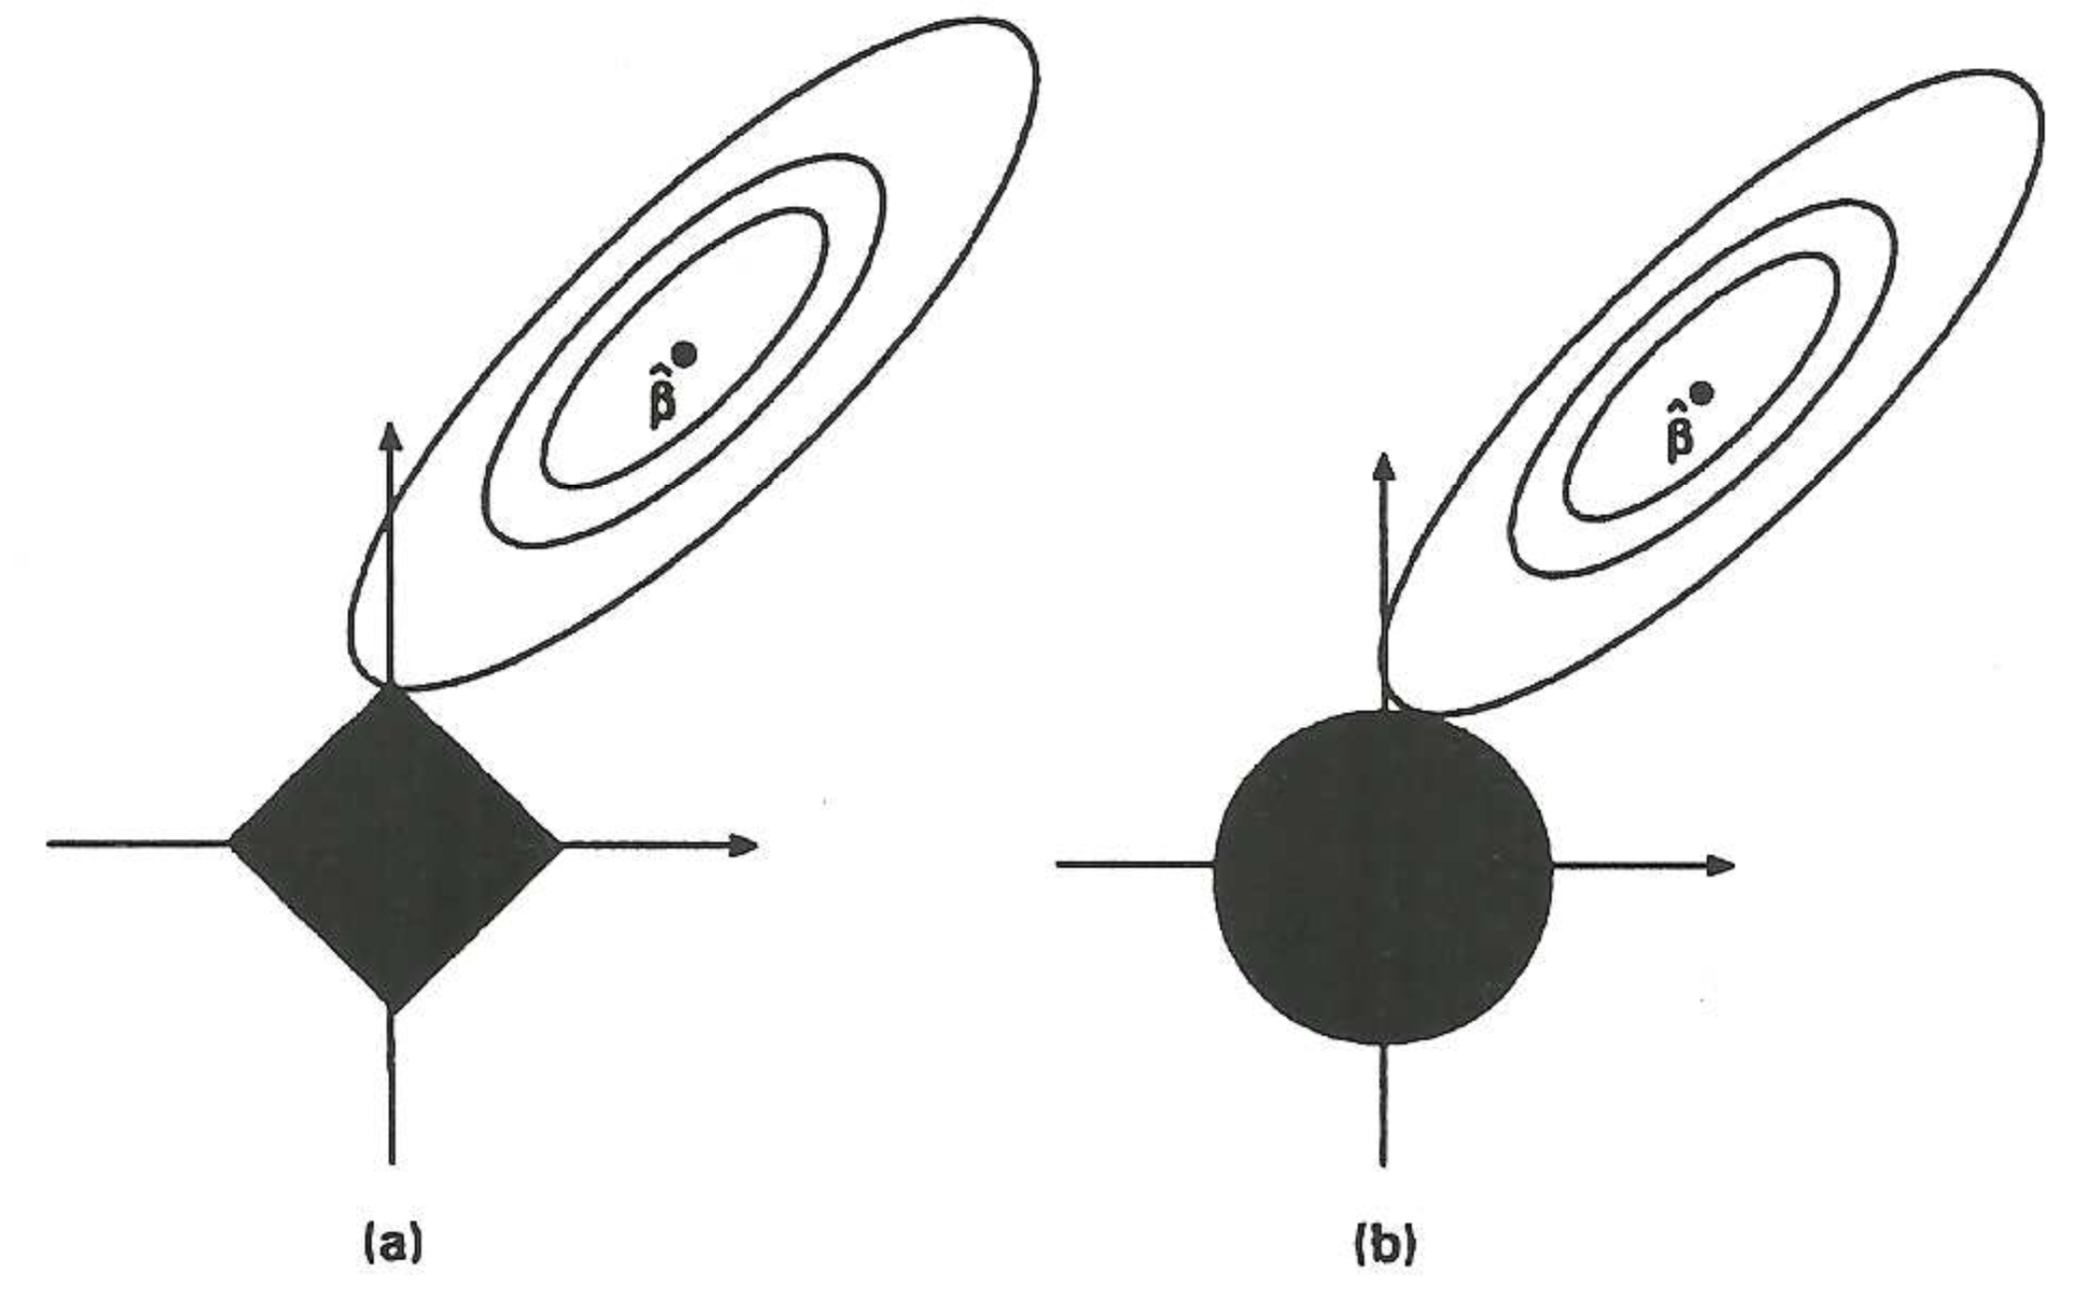
\includegraphics[scale=0.35]{linreg_lasso_level_set.png}
\caption{Level sets of least squares loss function with feasible sets for (a) lasso and (b) ridge regression in the case of \(\beta \in \mathbb{R}^2\).}
\label{linreg.lasso.level.set.figure}
\end{center}
\end{figure}

%%%%%%%%% 2018 Question 5

\begin{proposition}[\textbf{2018 DSO Statistics Group In-Class Screening Exam, Question 5}]\label{linreg.prop.2018.screen.5}

Consider the optimization problem 

\begin{equation}\label{2018.screen.5.a.objective}
\begin{aligned}
& \underset{\beta \in \mathbb{R}^p}{\text{minimize}}
& & \frac{1}{2} \lVert y - X \beta \rVert_2^2 + \lambda \lVert \beta \rVert_1
\end{aligned}
\end{equation}

where \(y \in \mathbb{R}^n, X \in \mathbb{R}^{n \times p}\), and \(\lambda > 0\). 

\begin{enumerate}[(a)]

\item The following problem is a dual of (\ref{2018.screen.5.a.objective}):

\[
\begin{aligned}
& \underset{u \in \mathbb{R}^n}{\text{maximize}}
& & \frac{1}{2} \lVert y  \rVert_2^2 - \frac{1}{2} \lVert y  - u \rVert_2^2 
& \text{subject to}
& & \lVert X^T u \rVert_\infty \leq \lambda.
\end{aligned}
\]

Also, \(\hat{u} = y - X \hat{\beta}\), where \(\hat{\beta}\) is a solution of (\ref{2018.screen.5.a.objective}) and \(\hat{u}\) is a solution of the dual.

\item \(\hat{\beta}\) is not necessarily unique, but \(\hat{u}\), \(\lVert y - X \hat{\beta} \rVert_2^2\), and \(\lVert \hat{\beta} \rVert_1\) are.

\item Suppose \(y = X \beta^* + \epsilon\), and suppose the tuning parameter \(\lambda\) is chosen to satisfy \(\lambda \geq \lVert X ^T \epsilon \rVert_\infty\). Then

\begin{enumerate}[(i)]

\item 

\[
\frac{1}{2} \lVert y - X \hat{\beta} \rVert_2^2 + \lambda \lVert \hat{\beta} \rVert_1 \leq \frac{1}{2} \lVert \epsilon \rVert_2^2 + \lambda \lVert \beta^* \rVert_1.
\]

\item 

\[
\frac{1}{2} \lVert y - X \hat{\beta} \rVert_2^2 + \lambda \lVert \hat{\beta}\rVert_1 \geq \frac{1}{2} \lVert y \rVert_2^2 - \frac{1}{2} \lVert X \beta^* \rVert_2^2.
\]

\item 

\[
\frac{1}{2} \lVert y - X \hat{\beta} \rVert_2^2 + \lambda \lVert \hat{\beta} \rVert_1 \geq \frac{1}{2} \lVert \epsilon \rVert_2^2 - \lambda \lVert \beta^* \rVert_1.
\]

\end{enumerate}

\end{enumerate}

\end{proposition}

\begin{remark}

We can express the original optimization problem (\ref{2018.screen.5.a.objective}) as 

\begin{equation}\label{2018.screen.5.a.objective.alt}
\begin{aligned}
& \underset{\beta \in \mathbb{R}^p, z \in \mathbb{R}^n}{\text{minimize}}
& & \frac{1}{2} \lVert y - z \rVert_2^2 + \lambda \lVert \beta \rVert_1 \\
& \text{subject to}
& & z = X \beta.
\end{aligned}
\end{equation}

We will also refer to another expression of the lasso optimization problem,

\begin{equation}\label{2018.screen.5.a.objective.orig}
\begin{aligned}
& \underset{\beta \in \mathbb{R}^p}{\text{minimize}}
& & \frac{1}{2} \lVert y - X \beta \rVert_2^2 \\
& \text{subject to}
& & \lVert\beta \rVert_1 \leq t
\end{aligned}
\end{equation}

for some \(t >0\). 

\end{remark}

Before proving the main results, we will show a few simpler results. Whenever \(\lambda > 0\), the lasso objective function (\ref{2018.screen.5.a.objective}) is the Lagrangian of (\ref{2018.screen.5.a.objective.orig}). We will prove a useful lemma about the relationship between these functions.

\begin{lemma}\label{2018.screen.5.b.iv.relation}
For a given \(\lambda >0\), let \(\hat{\beta}\) minimize (\ref{2018.screen.5.a.objective}). Then there is exactly one \(t = \lVert \hat{\beta} \rVert_1\) such that any \(\hat{\beta}\) minimizing (\ref{2018.screen.5.a.objective}) also minimizes (\ref{2018.screen.5.a.objective.orig}).

\end{lemma}

\begin{proof}
This must be true by contradiction. First of all, since the objective function of (\ref{2018.screen.5.a.objective.orig}) is continuous and the feasible region \(\lVert \beta \rVert_1 \leq t\) is compact, a minimum of (\ref{2018.screen.5.a.objective.orig}) is guaranteed to exist. Now suppose \(\hat{\beta}\) minimizes (\ref{2018.screen.5.a.objective}) for a fixed \(\lambda\), with \(\lVert \hat{\beta} \rVert_1 = t\), but there is a different solution \(\hat{\beta}^*\) that is feasible for (\ref{2018.screen.5.a.objective.orig}) and achieves a lower value. That is,

\[
\frac{1}{2} \lVert y - X \hat{\beta}^* \rVert_2^2  < \frac{1}{2} \lVert y - X \hat{\beta} \rVert_2^2.
\]

and \(\lVert\hat{\beta}^*\rVert_1 \leq \lVert\hat{\beta}\rVert_1 = t\). Since \(\lambda > 0\), \(\lVert\hat{\beta}\rVert_1 < \lVert \hat{\beta}_{global} \rVert_1\), where \(\hat{\beta}_{global}\) is a global minimum for \(\frac{1}{2} \lVert y - X \hat{\beta} \rVert_2^2\). Since (\ref{2018.screen.5.a.objective.orig}) is convex and all global minima lie outside the feasible region, \(\hat{\beta}^*\) lies on the boundary; that is, \(\lVert \hat{\beta}^* \rVert_1 = \lVert\hat{\beta}\rVert_1 = t\). But then

\[
\frac{1}{2} \lVert y - X \hat{\beta}^* \rVert_2^2  < \frac{1}{2} \lVert y - X \hat{\beta} \rVert_2^2 \iff \frac{1}{2} \lVert y - X \hat{\beta}^* \rVert_2^2 + \lambda \lVert\hat{\beta}^* \rVert_1 < \frac{1}{2} \lVert y - X \hat{\beta} \rVert_2^2 +  \lambda \lVert\hat{\beta} \rVert_1
\]

which contradicts the fact that \(\hat{\beta}\) minimizes (\ref{2018.screen.5.a.objective}). 

\end{proof}

Another useful result follows in a simple way from Lemma \ref{2018.screen.5.b.iv.relation}.

\begin{proposition}\label{linreg.2018.screen.5.b.iv.prop}
Let \(\mathcal{B}\) be the set of all \(\hat{\beta}\) that minimize (\ref{2018.screen.5.a.objective}) for some fixed \(\lambda > 0\). Then for any two \(\hat{\beta}_1, \hat{\beta}_2 \in \mathcal{B}\), \(\lVert \hat{\beta}_1 \rVert_1 = \lVert \hat{\beta}_2 \rVert_1\). That is, \(\lVert \hat{\beta} \rVert_1\) is unique.
\end{proposition}

\begin{proof}
Suppose \(\hat{\beta}_1\) and \(\hat{\beta}_2\) both minimize (\ref{2018.screen.5.a.objective}), and (without loss of generality) \(\lVert \hat{\beta}_1 \rVert_1 < \lVert \hat{\beta}_2 \rVert_1\). By Lemma \ref{2018.screen.5.b.iv.relation}, these values both minimize (\ref{2018.screen.5.a.objective.orig}) with \(t =  \lVert \hat{\beta}_2 \rVert_1\) (we cannot choose \(t =  \lVert \hat{\beta}_1 \rVert_1\) because \(\hat{\beta}_1\) is not feasible for that problem). Because the global minimum of (\ref{2018.screen.5.a.objective.orig}) lies outside the feasible region and  (\ref{2018.screen.5.a.objective.orig}) is convex, all solutions to (\ref{2018.screen.5.a.objective.orig}) lie on the boundary of the feasible region. But \(\lVert\hat{\beta}_1 \rVert_1 < \lVert \hat{\beta}_2 \rVert_1\), so \(\hat{\beta}_1\) is not on the boundary of the feasible region, contradiction. Therefore \(\lVert \hat{\beta}_1 \rVert_1 = \lVert \hat{\beta}_2 \rVert_1\) for all solutions \(\hat{\beta}_1\), \(\hat{\beta}_2\) to (\ref{2018.screen.5.a.objective}); that is,  \(\lVert \hat{\beta} \rVert_1\) is unique. (See \citet{Osborne2000} for more details.)

\end{proof}

Now we are ready to prove Proposition \ref{linreg.prop.2018.screen.5}.

\begin{proof}[Proof of Proposition \ref{linreg.prop.2018.screen.5}]

\begin{enumerate}[(a)]

\item

The Lagrangian of (\ref{2018.screen.5.a.objective.alt}) is

\[
\mathcal{L}(\beta, z, u) = \frac{1}{2} \lVert y - z \rVert_2^2 + \lambda \lVert \beta \rVert_1 + u^T(z - X \beta),
\]

so the Lagrange dual function is

\[
\inf_{\beta, z} \left\{ \mathcal{L}(x, u)\right\}  = \inf_{\beta, z} \left\{\frac{1}{2} \lVert y - z \rVert_2^2 + \lambda \lVert \beta \rVert_1 + u^T(z - X \beta)  \right\}
\]

\[
= \inf_{\beta, z} \left\{\frac{1}{2} (y-z)^T(y-z) + u^T z + \lambda \lVert \beta \rVert_1  - u^T X \beta  \right\} 
\]

This minimization is separable:

\begin{equation}\label{2018.screen.5.a.a}
= \inf_{z} \left\{\frac{1}{2} \left(y^Ty - 2 y^Tz + z^Tz \right) + u^T z \right\} + \inf_{\beta} \left\{ \lambda \lVert \beta \rVert_1  - u^T X \beta  \right\}
\end{equation}

We will handle each part of (\ref{2018.screen.5.a.a}) separately. First, the left side:

\[
 \inf_{z} \left\{\frac{1}{2} \left(y^Ty - 2 y^Tz + z^Tz \right) + u^T z \right\} = \inf_{z} \left\{\frac{1}{2}z^Tz  + (u - y)^Tz + \frac{1}{2} y^Ty   \right\} 
\]

Since this is a convex quadratic form, differentiate with respect to \(z\) and set equal to zero:

\begin{equation}\label{2018.screen.5.a.other.part.result}
z + (u - y) = 0 \implies z = y - u
\end{equation}

\[
 \implies \inf_{z} \left\{\frac{1}{2}z^Tz  + (u - y)^Tz + \frac{1}{2} y^Ty   \right\} =  \frac{1}{2}(y - u) ^T(y - u)  + (u - y)^T(y - u) + \frac{1}{2} y^Ty 
\]

\[
=  \frac{1}{2}\left(y^Ty -2 u^Ty + u^Tu \right)  + 2u^Ty - y^Ty - u^Tu + \frac{1}{2} y^Ty  = -\frac{1}{2}u^Tu   + u^Ty = \frac{1}{2} y^Ty - \frac{1}{2}y^Ty  + u^Ty - \frac{1}{2} u^Tu 
\]

\[
= \frac{1}{2} y^Ty - \frac{1}{2}(y^Ty - 2u^Ty + u^Tu ) = \frac{1}{2} y^Ty - \frac{1}{2}(y - u)^T(y - u)= \frac{1}{2} \lVert y \rVert_2^2 - \frac{1}{2} \lVert y - u \rVert_2^2 
\]

Next we will minimize the right side of (\ref{2018.screen.5.a.a}):

\[
 \inf_{\beta} \left\{ \lambda \lVert \beta \rVert_1  - u^T X \beta  \right\} =  \inf_{\beta} \left\{ \lambda \sum_{i=1}^p | \beta_i| - \sum_{i=1}^p \begin{bmatrix} u^T X \end{bmatrix}_i  \beta_i  \right\}  =  \inf_{\beta} \left\{ \sum_{i=1}^p  \left( \lambda  | \beta_i| -  \begin{bmatrix} u^T X \end{bmatrix}_i  \beta_i \right)  \right\} 
 \]
 
% \[
% = \begin{cases}
%   \inf_{\beta} \left\{ \sum_{i=1}^p  \left( \lambda  | \beta_i| -  \begin{bmatrix} u^T X \end{bmatrix}_i  \beta_i \right)  \right\} & \beta_i 
%   \end{cases}
% \]
 
 \[
 =  \inf_{\beta} \left\{ \sum_{i=1}^p  \left(\operatorname{sgn}(\beta_i) \lambda-  \begin{bmatrix} u^T X \end{bmatrix}_i  \right)    \beta_i  \right\}   =  \sum_{i=1}^p  \inf_{\beta_i} \left\{ \left(\operatorname{sgn}(\beta_i) \lambda-  \begin{bmatrix} u^T X \end{bmatrix}_i  \right)    \beta_i  \right\} .
 \]
 
Notice that when \(\beta_i\) is negative, if \(\left(\operatorname{sgn}(\beta_i) \lambda-  \begin{bmatrix} u^T X \end{bmatrix}_i  \right) =  -\left(\lambda+  \begin{bmatrix} u^T X \end{bmatrix}_i  \right)\) is positive there is no lower bound on the quantity we are minimizing; otherwise, when \(\beta_i\) is negative the infimum is 0. When \(\beta_i\) is positive, if  \(\left(\operatorname{sgn}(\beta_i) \lambda-  \begin{bmatrix} u^T X \end{bmatrix}_i  \right) =  \left(\lambda-  \begin{bmatrix} u^T X \end{bmatrix}_i  \right)\) is negative there is no lower bound on the quantity we are minimizing; otherwise, when \(\beta_i\) is negative the infimum is 0. That is, the only dual feasible points satisfy for all \(i\)

\[
  -\left(\lambda+  \begin{bmatrix} u^T X \end{bmatrix}_i  \right) \leq 0, \qquad \lambda-  \begin{bmatrix} u^T X \end{bmatrix}_i   \geq 0 \iff \begin{bmatrix} u^TX\end{bmatrix}_i \geq -\lambda, \qquad \begin{bmatrix} u^TX\end{bmatrix}_i \leq \lambda
\]

which is equivalent to the condition
\[
\lVert u^TX \rVert_\infty \leq \lambda.
\]

Therefore the Lagrange dual function is


\begin{equation}\label{2018.screen.5.a.dual}
 \inf_{\beta, z} \left\{ \mathcal{L}(x, u)\right\}  = \frac{1}{2} \lVert y \rVert_2^2 - \frac{1}{2} \lVert y - u \rVert_2^2 
\end{equation}

subject to the constraint \(\lVert u^TX \rVert_\infty \leq \lambda\). This quantity represents a lower bound on the minimum value of the original optimization problem for all \(u \in \mathbb{R}^p\). The dual problem is to find the best lower bound by maximizing over \(u\); that is, the dual problem is

\begin{equation}\label{2018.screen.5.a.dual.ans}
\begin{aligned}
& \underset{u \in \mathbb{R}^p}{\text{maximize}}
& & \frac{1}{2} \lVert y \rVert_2^2 - \frac{1}{2} \lVert y - u \rVert_2^2  \\
& \text{subject to}
& & \lVert u^TX \rVert_\infty \leq \lambda.
\end{aligned}
\end{equation}

Lastly, suppose \(\hat{\beta}\) and \(\hat{u}\) satisfy

\[
\hat{\beta} = 
\begin{aligned}
& \underset{\beta \in \mathbb{R}^p}{\arg \min}
& & \frac{1}{2} \lVert y - X \beta \rVert_2^2 + \lambda \lVert \beta \rVert_1
\end{aligned},
\]

\[
 \qquad \hat{u} = 
\begin{aligned}
& \underset{u \in \mathbb{R}^p}{\arg \max}
& & \frac{1}{2} \lVert y \rVert_2^2 - \frac{1}{2} \lVert y - u \rVert_2^2  \\
& \text{subject to}
& & \lVert u^TX \rVert_\infty \leq \lambda
\end{aligned} = 
\begin{aligned}
& \underset{u \in \mathbb{R}^p}{\arg \min}
& & -\frac{1}{2} \lVert y \rVert_2^2 + \frac{1}{2} \lVert y - u \rVert_2^2  \\
& \text{subject to}
& & \lVert u^TX \rVert_\infty \leq \lambda
\end{aligned}
\]

Then since (\ref{2018.screen.5.a.other.part.result}) is a requirement for dual feasibility of \(u\) and strong duality applies, we have \(\hat{u} = y - X \hat{\beta}\).

\begin{remark}

Note that we could also find the arguments maximizing (\ref{2018.screen.5.a.dual.ans}) by

\[
\begin{aligned}
& \underset{u \in \mathbb{R}^p}{\arg \min}
& & -\frac{1}{2} \lVert y \rVert_2^2 + \frac{1}{2} \lVert y - u \rVert_2^2  \\
& \text{subject to}
& & \lVert u^TX \rVert_\infty \leq \lambda.
\end{aligned} = \begin{aligned}
& \underset{u \in \mathbb{R}^p}{\arg \min}
& &  \frac{1}{2} \lVert y - u \rVert_2^2  \\
& \text{subject to}
& & \lVert u^TX \rVert_\infty \leq \lambda.
\end{aligned}
\]

where the first step follows from the fact that arguments that maximize a function are the same as the arguments that minimize the negative of a function, and the second step follows from the fact that the \( -\frac{1}{2} \lVert y \rVert_2^2\) term does not include \(u\). Therefore we see that the residual vector \(u\) from a lasso fit can be thought of as the projection of \(y\) onto the convex polyhedron \(C \subset \mathbb{R}^n\) defined by \(C := \{u: \lVert X^Tu \rVert_\infty \leq \lambda \}\).

Another way of saying this is that the lasso estimate \(\hat{y} = X \hat{\beta}_{\text{lasso}}\) itself is the residual from projecting \(y\) onto \(C\); that is,

\[
X \hat{\beta}_{\text{lasso}} = (I - P_C)y,
\]

where \(P_C\) is the operator projecting \(y\) onto \(C\).

\end{remark}

\item

\begin{enumerate}[(i)]

% 5(b)i
\item \textbf{Not necessarily unique.} Per \citet{Tibshirani2013}, if \(\operatorname{rank}(X) < p\), the lasso solution is not necessarily unique. Intuitively, this is because the columns of \(X\) are linearly dependent, so there may exist more than one linear combination of the columns that minimizes (\ref{2018.screen.5.a.objective}). \textbf{Jacob's suggestion: counterexample. X is two columns that are equal; then convex combinations of two solutions are equal as long as same sign (can't be opposite sign because then \(\ell_1\) could be smaller by setting one equal to 0.}

% 5(b)ii
\item \textbf{Necessarily unique.} The dual problem (\ref{2018.screen.5.a.dual.ans}) is strictly concave, so the value \(\hat{u}\) that maximizes it is unique.

%  \textbf{flesh out more} By a result from part (a), \(\hat{u} = y - X \hat{\beta}\). By part (iii), even though \(\hat{\beta}\) is not unique, \(X \hat{\beta}\) is (see also Lemma 1 in \citet{Tibshirani2013}). Therefore \(\hat{u}\) is unique.

%\textbf{Jacob's solution: strictly convex optimization problem, so argument maximizing is unique. dual is always convex; } 

% 5(b)iii
\item \textbf{Necessarily unique} (except in the trivial case \(\lambda=0\)). Per part 5(b)(iv), \(\lVert \hat{\beta} \rVert_1\) is unique. (\ref{2018.screen.5.a.objective}) is convex, so the minimum \(\frac{1}{2} \lVert y - X \hat{\beta} \rVert_2^2 + \lambda \lVert \hat{\beta} \rVert_1\) is unique. Therefore \( \lVert y - X \hat{\beta} \rVert_2^2\) must be unique.

\textbf{Jacob's solution:} Since \(\hat{u}\) is unique and by (\ref{2018.screen.5.a.other.part.result}) \(\hat{u} = y - X \hat{\beta}\), we must have that \(\lVert \hat{u} \rVert = \lVert y - X \hat{\beta} \rVert\) is unique.

%\textbf{Necessarily unique.} The optimization problem is convex in \(\beta\), so it has a unique minimum value \(\frac{1}{2} \lVert y - X \hat{\beta} \rVert_2^2 + \lambda \lVert \hat{\beta} \rVert_1\). 

% 5(b)iv
\item \textbf{Necessarily unique} (except in the trivial case \(\lambda=0\)). This is immediate from Proposition \ref{linreg.2018.screen.5.b.iv.prop}.


\end{enumerate}

% 5c
\item 

\begin{enumerate}[(i)]

% 5(c)i
\item Since \(\beta^*\) is clearly feasible for (\ref{2018.screen.5.a.objective}) and \(\hat{\beta}\) achieves the minimum, we have

\[
\frac{1}{2} \lVert y - X \beta^* \rVert_2^2 + \lambda \lVert \beta^* \rVert_1 \geq \frac{1}{2} \lVert y - X \hat{\beta} \rVert_2^2 + \lambda \lVert \hat{\beta} \rVert_1 \iff  \frac{1}{2} \lVert y - X \hat{\beta} \rVert_2^2 + \lambda \lVert \hat{\beta} \rVert_1 \leq \frac{1}{2} \lVert\epsilon \rVert_2^2 + \lambda \lVert \beta^* \rVert_1
\]


% 5(c)ii
\item

% \textbf{Jacob's solution: plug in \(\epsilon\) for \(u\) in the lower bound equation, then you get \(X \beta^*\)}

We know that the expression in the dual problem (\ref{2018.screen.5.a.dual.ans}) is a lower bound for the solution of the primal problem (\ref{2018.screen.5.a.objective}) for any \(u\) feasible for (\ref{2018.screen.5.a.dual.ans}) (that is, any \(u\) satisfying \(\lVert u^TX \rVert_\infty \leq \lambda\)). Therefore we have

\[
\frac{1}{2} \lVert y - X \hat{\beta} \rVert_2^2 + \lambda \lVert \beta \rVert_1 \geq  \frac{1}{2} \lVert y \rVert_2^2 - \frac{1}{2} \lVert y - u \rVert_2^2.
\]

Since by assumption \(\lambda \geq \lVert X^T \epsilon \rVert_\infty\), \(\epsilon\) is feasible for (\ref{2018.screen.5.a.dual.ans}). Therefore we have

\begin{equation}\label{2018.screen.5.c.ii.result}
\frac{1}{2} \lVert y - X \hat{\beta} \rVert_2^2 + \lambda \lVert \beta \rVert_1 \geq  \frac{1}{2} \lVert y \rVert_2^2 - \frac{1}{2} \lVert y - \epsilon \rVert_2^2 =  \frac{1}{2} \lVert y \rVert_2^2 - \frac{1}{2} \lVert X \beta^* \rVert_2^2
\end{equation}

as desired.


\item 



We can rewrite the right side of (\ref{2018.screen.5.c.ii.result}) as 

\begin{equation}\label{2018.screen.5.c.ii.result.rewritten}
\frac{1}{2} \lVert y \rVert_2^2 - \frac{1}{2} \lVert X \beta^* \rVert_2^2 = \frac{1}{2} \lVert X \beta^* \rVert_2^2 + \frac{1}{2} \lVert \epsilon \rVert_2^2 + \epsilon^T X \beta^* - \frac{1}{2} \lVert X \beta^* \rVert_2^2  =  \frac{1}{2} \lVert \epsilon \rVert_2^2 + \epsilon^T X \beta^*. 
\end{equation}

By assumption, we have 
\[
\lambda \geq \lVert X^T \epsilon \rVert_\infty \iff \lambda \boldsymbol{1}  - X^T \epsilon \succeq 0 \implies \lambda \boldsymbol{1} \beta^*  - X^T \epsilon \beta^* \succeq 0 
\]

\[
\iff - \lambda \lVert \beta^* \rVert_1 \leq \epsilon^T X \beta^* \leq \lambda \lVert \beta^* \rVert_1.
\]

By H\"{o}lder's Inequality, we have for any two vectors \(u, v \in \mathbb{R}^n\), \( | u^Tv | \leq \lVert u \rVert_\infty \lVert v \rVert_1\). Therefore

\[
| \epsilon^T X \beta^*| = | (X^T \epsilon)^T \beta^* | \leq \lVert X^T \epsilon \rVert_\infty \lVert \beta^* \rVert_1 \leq \lambda \lVert \beta^* \rVert_1
\]

where the last step used the assumption \(\lVert X^T \epsilon \rVert_\infty \leq \lambda\). So we have 

\[
 \frac{1}{2} \lVert \epsilon \rVert_2^2 +\lambda \lVert \beta^* \rVert_1 \leq \frac{1}{2} \lVert \epsilon \rVert_2^2 + \epsilon^T X \beta^* .
\]

Substituting in to (\ref{2018.screen.5.c.ii.result}), using the identity in (\ref{2018.screen.5.c.ii.result.rewritten}), and using the result from part 5(c)(iii) yields

\[
 \frac{1}{2} \lVert \epsilon \rVert_2^2 +\lambda \lVert \beta^* \rVert_1 \leq \frac{1}{2} \lVert \epsilon \rVert_2^2 + \epsilon^T X \beta^* = \frac{1}{2} \lVert y \rVert_2^2 - \frac{1}{2} \lVert X \beta^* \rVert_2^2  \leq \frac{1}{2} \lVert y - X \hat{\beta} \rVert_2^2 + \lambda \lVert \beta \rVert_1 
\]

as desired.

% 5(c)iv
\item  We see from parts (i) and (iii) that

\[
\frac{1}{2} \lVert y - X \hat{\beta} \rVert_2^2 + \lambda \lVert \beta \rVert_1 - \lambda \lVert \beta^* \rVert_1  \leq \frac{1}{2} \lVert \epsilon \rVert_2^2 \leq  \frac{1}{2} \lVert y - X \hat{\beta} \rVert_2^2 + \lambda \lVert \beta \rVert_1 + \lambda \lVert \beta^* \rVert_1 
\]

\[
\iff \frac{1}{n} \lVert y - X \hat{\beta} \rVert_2^2 + \frac{2}{n} \lambda \lVert \beta \rVert_1 - \frac{2}{n}\lambda \lVert \beta^* \rVert_1  \leq \frac{1}{n} \lVert \epsilon \rVert_2^2 \leq  \frac{1}{n} \lVert y - X \hat{\beta} \rVert_2^2 + \frac{2}{n}\lambda \lVert \beta \rVert_1 +\frac{2}{n} \lambda \lVert \beta^* \rVert_1 
\]

that is, we can lower bound and upper bound \(\frac{1}{n} \lVert \epsilon \rVert_2^2 \) by taking the quantity \(\frac{1}{n} \lVert y - X \hat{\beta} \rVert_2^2 + \frac{2}{n} \lambda \lVert \beta \rVert_1\) and adding or subtracting \(\frac{2}{n}\lambda \lVert \beta^* \rVert_1\). Therefore it seems that the quantity in the middle of this interval,  \(\frac{1}{n} \lVert y - X \hat{\beta} \rVert_2^2 + \frac{2}{n} \lambda \lVert \beta \rVert_1\), is a reasonable estimator for \(\sigma^2 = \E \left[ n^{-1} \lVert \epsilon \rVert_2^2 \right]\).

\end{enumerate}

\end{enumerate}

\end{proof}



\subsection{Non-Negative Garotte}

This idea inspired the lasso. Proposed by \citet{Breiman1995}. It minimizes

\[
\sum_{i=1}^n \left(y_i - \alpha - \sum_{j=1}^p c_j \hat{\beta}_j^o x_{ij} \right)^2 \text{ subject to } c_j \geq 0, \sum_{j=1}^p c_j \leq t
\]

It starts with OLS estimates and shrinks them by non-negative factors whose sum is constrained. It depends on both the sign and magnitude of OLS estimates. In contrast, lasso avoids the explicit use of OLS estimates.

\subsection{LARS---Preliminaries and Intuition}\label{lars.prelims}

Intuition: the algorithm takes steps from a model where all coefficients are 0 to the biggest model (the unpenalized OLS model). Covariates are considered from the highest correlation with \(y\) to the least. (The variable most highly correlated with \(y\) is the one at the ``least angle" from \(y\).) Recall the original definition of the lasso estimator:

\begin{equation}\label{linreg.lasso.constrained}
\hat{\beta}_{lasso} = \underset{\beta \in \mathbb{R}^p}{\arg \min}\left\{ \frac{1}{2n}\lVert y - X \beta \rVert_2^2 \right\} \text{ subject to } \lVert \beta \rVert_1 \leq t
\end{equation}

The more common version now:

\begin{equation}\label{linreg.lasso.lagrangian}
\hat{\beta}_{lasso} =\underset{\beta \in \mathbb{R}^p}{\arg \min} \left\{ \frac{1}{2n}\lVert y - X \beta \rVert_2^2   + \lambda \lVert \beta \rVert_1 \right\}
\end{equation}

One form can be changed to the other by applying Lagrangians\footnote{However, the correspondence between \(t\) and \(\lambda\) is \textbf{not} one-to-one. Because with \(t = \infty\), \(\lambda =0\). But a slightly smaller \(t\) would result in the same solution.}. Have to be careful because this is a convex program (quadratic with ``linear" constraint---use a slack variable). 

Taking the gradient of the loss function in (\ref{linreg.lasso.lagrangian}) yields

\[
\nabla \bigg(  \frac{1}{2n}\lVert y - X \beta \rVert_2^2   + \lambda \lVert \beta \rVert_1 \bigg) = \nabla   \bigg( \frac{1}{2n}\lVert y - X \beta \rVert_2^2   \bigg) + \lambda \nabla \big( \lVert \beta \rVert_1 \big)
\]

\begin{equation}\label{linreg.lasso.lagrangian.gradient}
= - \frac{1}{n} X^T(y - X \beta) + \lambda \nabla  \big( \lVert \beta \rVert_1 \big)
\end{equation}

We set this equal to zero. If the first term equals 0, the residual has to equal 0. For the second part to equal zero, we have to account for the fact that the gradient doesn't exist at 0. In the one-dimensional case \(g(t) = |t|\), we have

\[
g'(t) = \begin{cases}
-1 & t < 0 \\
1 & t > 0
\end{cases}
\]

but it doesn't exist at 0. Instead of using the gradient, we will use \(\partial\), the subdifferential, which is the set of all subgradients. We have a solution if 0 is in the subdifferential. We can rewrite (\ref{linreg.lasso.lagrangian.gradient}) using the subdifferential instead of the gradient:

\[
\partial \bigg(  \frac{1}{2n}\lVert y - X \beta \rVert_2^2   + \lambda \lVert \beta \rVert_1 \bigg) = \nabla \bigg(  \frac{1}{2n}\lVert y - X \beta \rVert_2^2  \bigg)  + \lambda \partial \big( \lVert \beta \rVert_1 \big)  =  - \frac{1}{n} X^T(y - X \beta) + \lambda \partial \big( \lVert \beta \rVert_1 \big)
\]

Then rather than setting the gradient equal to 0, our condition is

\[
0 \in - \frac{1}{n} X^T(y - X \beta) + \lambda \partial \big( \lVert \beta \rVert_1 \big)
\]

Note that 

\[
\partial g (t) = \begin{cases}
-1 & t < 0 \\
[-1, 1] & t = 0 \\
1 & t > 0
\end{cases} = \begin{cases}
\operatorname{sgn}(t) & t \neq 0 \\
[-1, 1] & t = 0 
\end{cases}
\]

so we have

\begin{equation}\label{linreg.lasso.soln.cond}
0 \in - \frac{1}{n} X^T(y - X \beta) + \lambda \cdot \begin{bmatrix} \begin{cases}
\operatorname{sgn}(\beta_j) & t \neq 0 \\
[-1, 1] & \beta_j = 0 
\end{cases} \end{bmatrix}
\end{equation}

where 

\[
\begin{bmatrix} \begin{cases}
\operatorname{sgn}(\beta_j) & t \neq 0 \\
[-1, 1] & \beta_j = 0 
\end{cases} \end{bmatrix} \in \mathbb{R}^p
\]

is a vector with each entry as specified.

\begin{remark}
\begin{enumerate}[(1)]
\item Examining the \(j\)th component of the separable equation (\ref{linreg.lasso.soln.cond}), if \(\beta_j \neq 0\), we have

\[
0 = -\frac{1}{n} X_j^T(y - X \beta) + \lambda \cdot
\operatorname{sgn}(\beta_j) \iff \frac{1}{n} X_j^T(y - X \beta) = \lambda \cdot
\operatorname{sgn}(\beta_j) 
\]

Note that the left side contains the correlation between \(X_j\) and \(e = y - X \beta\), the residual vector. \textbf{So if lasso chooses \(k\) variables, all \(k\) of them will have the same correlation with the residual (\(\lambda\)).}

\item If \(\beta_j =0\), we have

\[
0 \in - \frac{1}{n} X^T(y - X \beta) + \lambda \cdot 
[-1, 1]  \iff \left|  \frac{1}{n} X^T(y - X \beta)  \right| \leq \lambda
\]

\textbf{So for unselected features, the (absolute) correlation should be bounded by \(\lambda\).}

\end{enumerate}

\end{remark}

These two conditions relate to the KKT conditions (first order conditions).

So if we start with \(\lambda\) very large and gradually decrease it, we will let in as the first feature the one that is most highly correlated with \(y\)---that is, the feature with the \textit{least angle} between it and \(y\).


\subsection{LARS}

\begin{figure}
\center{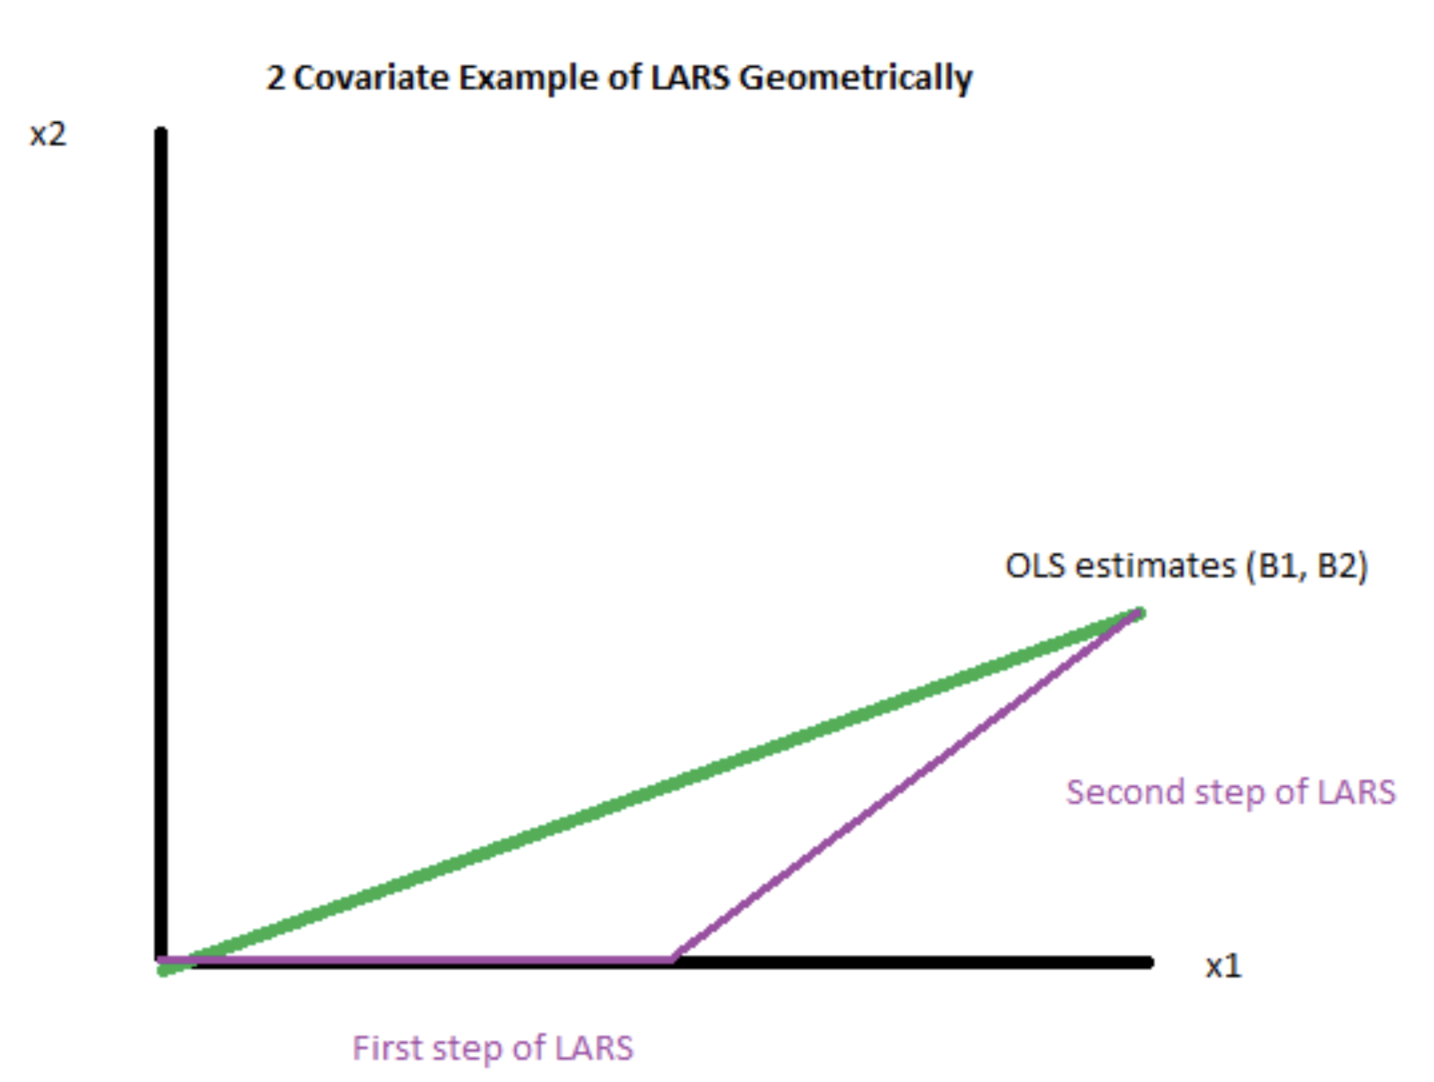
\includegraphics[width=0.8\textwidth, angle=0]{linreg_lars_2d.png}}
\caption{\label{fig:lars_2d} LARS figure in 2d case.}
\end{figure}

\begin{figure}
\center{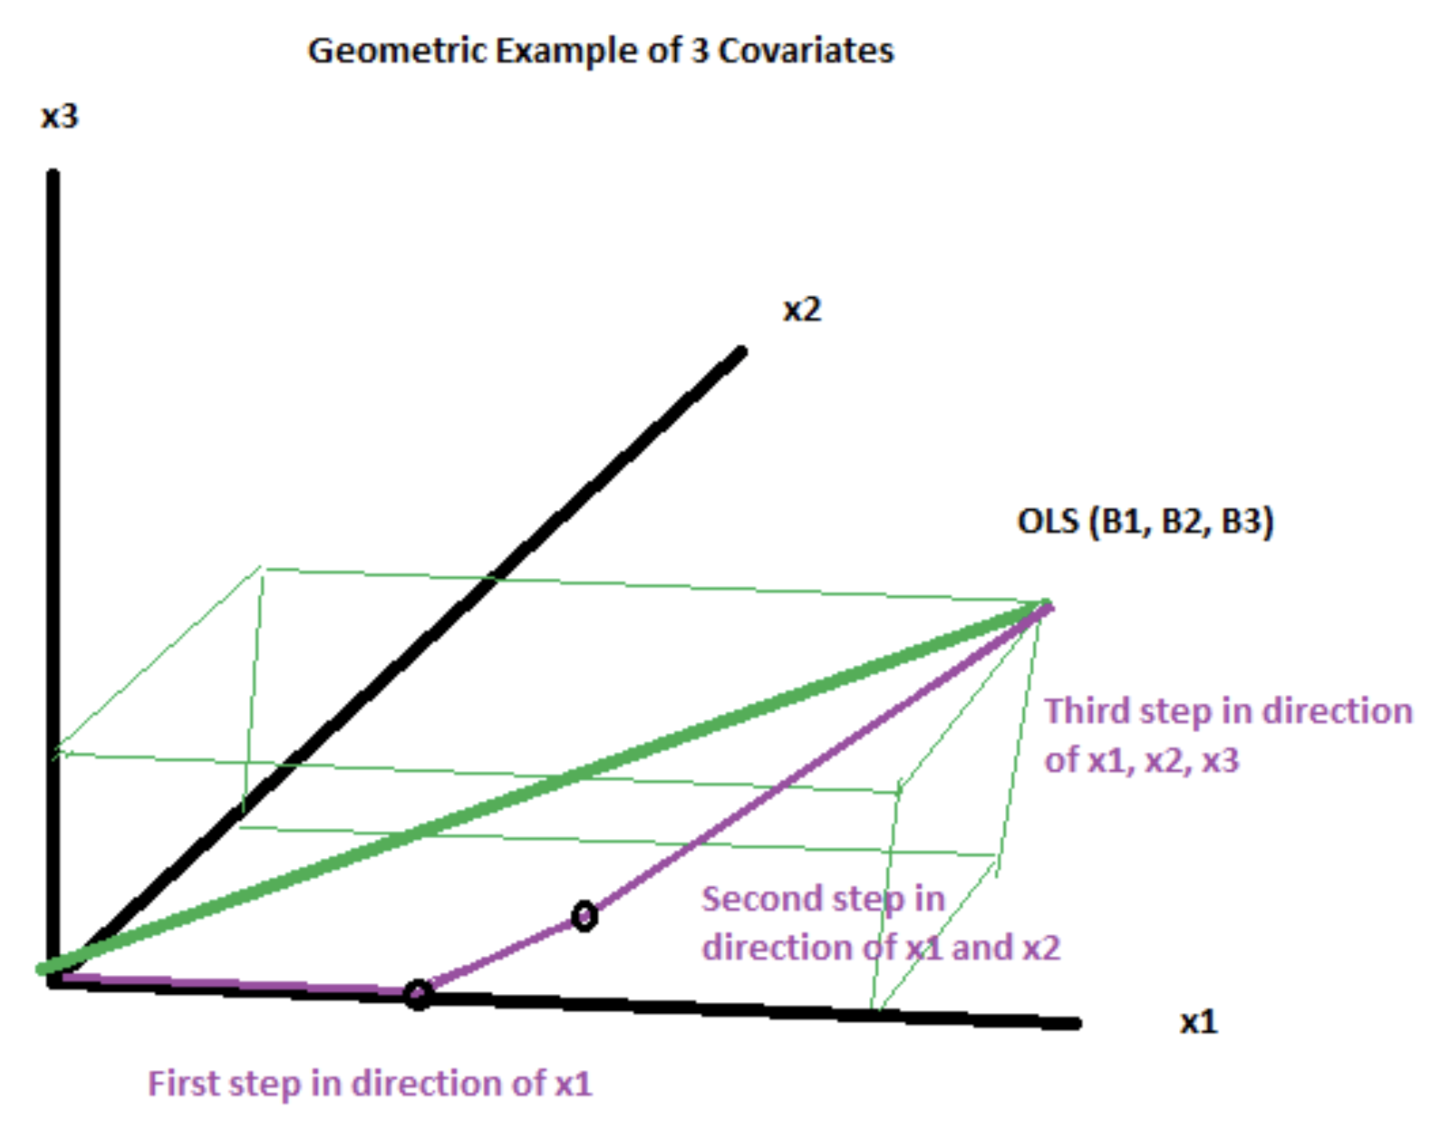
\includegraphics[width=0.8\textwidth, angle=0]{linreg_lars_3d.png}}
\caption{\label{fig:lars_3d} LARS figure in 3d case.}
\end{figure}

In Figure \ref{fig:lars_2d}, note that we choose feature \(X_1\) first because it has the highest correlation with \(y\). As the coefficient on \(X_1\) increases, the correlation between \(X_1\) and the residual with \(y\) decreases, while the correlation between \(X_2\) and the residual remains constant (\textbf{increases?}). When the correlation between \(X_1\) and the residual becomes equal to the correlation between \(X_2\) and the residual, \(X_2\) enters the lasso path.

\begin{remark} Just like in lasso, in LARS the correlation between all included features and the residual are equal (see the remark in Section \ref{lars.prelims}). However, LARS is a stepwise procedure---once we add a feature, it stays in the model. In the lasso, features can be dropped later in the path after they are selected---whenever \(\beta_j\) becomes 0, it is dropped from the current active set. A feature's sign cannot change in lasso---it is not possible. If we modify the LARS algorithm to have this property (``lasso modification"), then the result is the lasso estimator.

\end{remark}

The LARS algorithm for lasso has order \(\mathcal{O}(np \cdot \min \{n, p\})\). In particular, if \(p > n\) it has order \(\mathcal{O}(n^2p)\).


\section{Loss Functions}\label{linreg.sec.loss.fxs}

Asymmetric loss: may have asymmetry between overestimation and underestimation. For example: in a supply chain, estimate inventory level \(y_1, \ldots, y_n\). Let \(y_i = x_i' \beta + \epsilon_i\). Underestimating is really bad because then you don't have enough product for customers and they might not come back; overestimating not so bad. Then our loss function:

\[
\underset{\beta \in \mathbb{R}^p}{\min} \sum_{i=1}^n (1 - \tau) \underbrace{(y_i - x_i' \beta)_+}_{\text{under-estimation}} + \tau \underbrace{ (x_i' \beta - y_i)_+}_{\text{over-estimation}}
\]

you could choose \(\tau = 0.1\) for a 9 to 1 ratio of loss (i.e., underestimation is 9 times as costly as overestimation).

\begin{theorem}[\textbf{Loss: quadratic}]\label{exercise6.5}
Let $X:\Omega\to\mathbb{R}$ be a random variable with $\E X^{2}<\infty$. Then $\E(X-t)^{2}$ is minimized for $t\in\mathbb{R}$ uniquely when $t=\E X$.
\end{theorem}

\begin{proof}

%\textbf{proof definitely in Mostly Harmless Econometrics but might be less rigorous, possibly in Pesaran book, possible in stats 100C course notes.}

We seek

\[
 \arg \min_t \E(X - t)^2 = \arg \min_t \big[ \E(X^2) - 2t\E(X) + t^2 \big] = \arg \min_t \big[  t^2 - 2t\E(X)\big] 
\]

where the last step follows because \(\E(X^2)\) is independent of \(t\). This expression is quadratic in \(t\). Differentiating with respect to \(t\) and setting equal to 0, we have

\[
2t - 2 \E(X) = 0 \implies \boxed{\arg \min_t \E(X - t)^2 = \E(X)}
\]

\end{proof}

Huber loss: combines benefits of squared loss (unbiasedness) with MAD loss (robust).

\[
L_\delta^H(y, \hat{y}) = ( y - \hat{y})^2 \cdot I \left\{  |y - \hat{y}| \leq \delta \right\} 
+ | y - \hat{y}| \cdot I \left\{  |y - \hat{y}| > \delta \right\}.
\]

Only downside: not that easy to estimate (loss function is not differentiable). Instance of \textbf{M-estimation} (more generalized than regression):

\[
\hat{\beta}_M = \underset{\beta, \sigma}{\arg \min} \sum_{i=1}^n \rho_M \left(  \frac{y_i - x_i' \beta}{\sigma} \right)
\]

where \(\rho_M\) is a loss function. Suppose \(y_i = \sum_{j=1}^p x_{ij} \beta_j + \epsilon_i\). Then differentiating the loss function with respect to \(\beta\) yields

\[
\pderiv{}{\beta_k} \left[ \sum_{i=1}^n \rho_M \left(  \frac{y_i - x_i' \beta}{\sigma} \right) \right] = 0 \qquad \text{for } k \in \{1, \ldots, p\}.
\]

\[
= \sum_{i=1}^n \rho'(y_i - x_i' \beta) \cdot \frac{(- x_{ij}) }{\sigma} 
\]

Let \(u_i := (y_i - x_i' \beta)/\hat{\sigma}\). 

\[
\implies \sum_{i=1}^n \underbrace{ \frac{ \rho'(u_i)}{u_i} }_{\text{weight}} \cdot x_{ij} (y_i - x_i' \beta) = 0 
\]

Compare to least squares: normal equations \(X^T(y - X^T \beta_{OLS}) = 0\), or

\[
\sum_{i=1}^n x_{ij} (y_i - x_i' \beta) = 0 
\]

Now we have this extra weighting term. Algorithm for computing:

\begin{enumerate}

\item Use \(\hat{\beta}_{OLS}\) as the initial solution; then compute  

\[
u_i^{(0)} = \frac{ y_i' - x_i' \hat{\beta}_{OLS}}{\hat{\sigma}_{OLS}} 
\]

\item With \(w_i^{(0)} = \rho'(u_i)/u_i\), compute 

\[
\hat{\beta}_{LS}^{(1)} = (X^TW X)^{-1} X^T W y .
\]

\item Update weights with \(\hat{\beta}_{LS}^{(1)}\).

\item Repeat until convergence. (Convergence is a little tricky but should work.)

\end{enumerate}



For absolute deviation loss, see Section \ref{linreg.sec.quant.reg} on quantile regression.

\subsection{Feature Selection properties}

Model selection consistency: \(\Pr(\operatorname{supp}(\hat{\beta}) = \operatorname{supp}(\beta_0) ) \to 1\).

Oracle property: model selection consistency, asymptotic efficiency as efficient as if true model were known (``efficiency" having to do with the variance given \(n\)).

\begin{definition}[\textbf{Oracle property}] Let \(\beta^0\) denote the true parameter vector for data generated from a linear model. Let \(S_0\) be the true support; that is, \(S_0 = \{j: \beta_j^0 \neq 0, j = 1, \ldots, p\}\). Denote \(\hat{\beta}(\delta)\) the coefficient estimator for fitting procedure \(\delta\). We call \(\delta\) an \textbf{oracle procedure} if \(\hat{\beta}(\delta)\) asymptotically has the following properties:

\begin{itemize}

\item Identifies the right subset model (consistency): \(\{j: \hat{\beta}_j \neq 0\} = S_0\).

\item Has the optimal estimation rate: \(\sqrt{n}(\hat{\beta}(\delta)_{S_0} - \beta_{S_0}^0) \xrightarrow{d} \mathcal{N}(0, \Sigma_0)\) where \(\Sigma_0\) is the covariance matrix knowing the true subset model.

\end{itemize}

\end{definition}

The lasso problem is convex but not necessarily strictly convex if \(p > n\). That is, there is some flat region, so the minimizer may not be unique. Consider the KKT conditions from convex optimization:

\[
g(\beta) = \arg \min \left\{ \frac{1}{2n} \lVert y - X \beta \rVert_2^2 + \lambda \lVert \beta \rVert_1 \right\} =  \arg \min \left\{ f_1(\beta) + f_2(\beta) \right\}
\]

Then \(\hat{\beta}\) is a lasso solution if and only if 0 is in the subdifferential of \(g(\hat{\beta})\). Note that 

\[
\partial g(\hat{\beta}) = \nabla f_1 + \partial f_2 = \frac{1}{n} X^T(X \beta - y) + \lambda \begin{bmatrix}  \vdots \\ \partial | \beta_j | \\ \vdots \end{bmatrix} = \frac{1}{n} X^T(X \beta - y) + \lambda \begin{bmatrix}  \vdots \\ \begin{cases}  \operatorname{sgn}(\beta_j) & \beta_j \neq 0 \\ [-1, 1] & \beta_j = 0 \end{cases} \\ \vdots \end{bmatrix}
\]

Now assume \(\operatorname{supp}(\hat{\beta}) = \operatorname{supp}(\beta_0)\) (that is, assume lasso recovers the correct support). Suppose the first \(s\) features are nonzero and consider one of them (so we know that we should have \(\hat{\beta_j} \neq 0\)):

\[
0 \in \partial g(\hat{\beta}) \implies 0 \in \partial_j g(\hat{\beta}) = \bigg[ \frac{1}{n} X^T(X \beta - y) \bigg]_j + \lambda \operatorname{sgn}(\hat{\beta}_j) 
\]

Therefore

\begin{equation}\label{linreg.lasso.first.cond}
\frac{1}{n} X_A^T(X \hat{\beta} - y) + \lambda  \operatorname{sgn}(\hat{\beta}_j) = 0
\end{equation}

where \(X_A\) is a submatrix of \(X\) containing the columns corresponding to the features in the true support, is our first condition. Next, consider what happens for \(j > s\) (features not in the true support). We have

\[
0 \in \partial g(\hat{\beta}) \implies 0 \in \partial_j g(\hat{\beta}) = \bigg[ \frac{1}{n}X^T(X \beta - y) \bigg] + \lambda [-1, 1]
\]

\begin{equation}\label{linreg.lasso.bound.cond}
\implies \left\lVert \frac{1}{n} X_{A^C}^T (X \hat{\beta} - y) \right\rVert_\infty \leq \lambda
\end{equation}

where \(X_{A^C}\) is a submatrix of \(X\) containing the columns corresponding to the features not in the true support, is our boundary condition. Recall the true model

\[
y = X \beta_0 + \epsilon
\]

and consider the case \(X = \begin{bmatrix}X_1 & X_2 \end{bmatrix}\) where \(X_1\) are the features in the true model and \(X_2\) are noise features; that is, \(\beta_0 = \begin{bmatrix} \beta_1 \\ 0 \end{bmatrix}\). Then we are assuming

\[
\hat{\beta}_{\text{lasso}} = \begin{bmatrix} \hat{\beta_1} \\ 0 \end{bmatrix}.
\]

We have from (\ref{linreg.lasso.first.cond})

\[
0 = \frac{1}{n} X_1^T(X \hat{\beta} - y) + \lambda  \operatorname{sgn}(\hat{\beta}_1) = \frac{1}{n} X_1^T(X_1 \hat{\beta}_1 - X_1 \beta_1 - \epsilon) + \lambda  \operatorname{sgn}(\hat{\beta}_1) 
\]
% = \frac{1}{n}(  X_1^TX_1 \hat{\beta}_1 - X_1^TX_1 \beta_1 - X_1^T \epsilon) + \lambda  \operatorname{sgn}(\hat{\beta}_1)
\[
 \iff \frac{1}{n} X_1^TX_1 (\hat{\beta}_1 - \beta_1)  =  \frac{1}{n} X_1^T \epsilon - \lambda  \operatorname{sgn}(\hat{\beta}_1)
 \]
 
 Let's assume that \(\operatorname{sgn}(\hat{\beta}) = \operatorname{sgn}(\beta_0)\) (sign consistency).
 
 \[
  \iff \frac{1}{n} X_1^TX_1 (\hat{\beta}_1 - \beta_1)  =  \frac{1}{n} X_1^T \epsilon - \lambda  \operatorname{sgn}(\beta_1)
  \]
  
  which is linear in \(\hat{\beta}\). Solving, we have
  
\begin{equation}\label{linreg.lasso.first.cond.solved}
  \iff  \hat{\beta}_1 - \beta_1  =  ( X_1^TX_1)^{-1} \big( X_1^T \epsilon - n  \lambda  \operatorname{sgn}(\beta_1)\big)   \iff  \hat{\beta}_1   = \beta_1 +   ( n^{-1}X_1^TX_1)^{-1} \big( n^{-1} X_1^T \epsilon -   \lambda  \operatorname{sgn}(\beta_1) \big)
\end{equation}

Looking at the second (boundary) condition (\ref{linreg.lasso.bound.cond}), we have

\begin{equation}\label{linreg.lasso.bound.cond.cont}
\left\lVert \frac{1}{n} X_{2}^T (X \hat{\beta} - y) \right\rVert_\infty \leq \lambda.
\end{equation}

Consider that 

\[
X \hat{\beta}- y = X_1 \hat{\beta}_1 - X_1 \beta_1 - \epsilon = X_1(\hat{\beta}_1 - \beta_1) - \epsilon
\]

Substituting in the result from (\ref{linreg.lasso.first.cond.solved}) yields

\[
X \hat{\beta}- y  = X_1\big[  ( n^{-1} X_1^TX_1)^{-1} \big( n^{-1} X_1^T \epsilon -  \lambda  \operatorname{sgn}(\beta_1)\big)   \big] - \epsilon
\]

which when we plug into (\ref{linreg.lasso.bound.cond.cont}) yields

\[
\left\lVert \frac{1}{n} X_{2}^T \left[X_1  (n^{-1} X_1^TX_1)^{-1} \big( n^{-1} X_1^T \epsilon -  \lambda  \operatorname{sgn}(\beta_1)\big) - \epsilon\right] \right\rVert_\infty \leq \lambda.
\]

\[
\iff \left\lVert \frac{1}{n} X_{2}^T X_1 (n^{-1} X_1^TX_1)^{-1} \big( n^{-1} X_1^T \epsilon -  \lambda  \operatorname{sgn}(\beta_1)\big)    -  \frac{1}{n} X_{2}^T \epsilon \right\rVert_\infty \leq \lambda.
\]

Using the Triangle Inequality, we have

\[
\left\lVert \frac{1}{n} X_{2}^T X_1 (n^{-1} X_1^TX_1)^{-1} \big( n^{-1} X_1^T \epsilon -  \lambda  \operatorname{sgn}(\beta_1)\big)    -  \frac{1}{n} X_{2}^T \epsilon \right\rVert_\infty 
\]

\[
\leq \left\lVert \frac{1}{n} X_{2}^T X_1 (n^{-1} X_1^TX_1)^{-1} \big( n^{-1} X_1^T \epsilon -  \lambda  \operatorname{sgn}(\beta_1)\big)  \right\rVert_\infty + \left\lVert  \frac{1}{n} X_{2}^T \epsilon \right\rVert_\infty 
\]

\begin{equation}\label{linreg.lasso.bound.cond.cont.more}
\leq \left\lVert \frac{1}{n} X_{2}^T  X_1 (n^{-1} X_1^TX_1)^{-1} \right\rVert_\infty \cdot \left\lVert  n^{-1} X_1^T \epsilon -  \lambda  \operatorname{sgn}(\beta_1)    \right\rVert_\infty + \left\lVert  \frac{1}{n} X_{2}^T \epsilon \right\rVert_\infty 
\end{equation}

Assume that the \(j\)th column of \(X\) has \(L_2\) norm \(n^{1/2}\) (as it would if all entries equaled 1). We have

\[
\left\lVert n^{-1} X_1^T \epsilon \right\rVert_\infty \leq \lambda/2, \qquad \left\lVert n^{-1} X_2^T \epsilon \right\rVert_\infty \leq \lambda/2
\]

\[
\left\lVert n^{-1} X^T \epsilon \right\rVert_\infty \leq \lambda/2 \text{ with large probability}
\]

Recall that \(\lambda = \sigma \sqrt{ \frac{c \log p }{n} } \) for some \(c >2\). Then we have (continuing from (\ref{linreg.lasso.bound.cond.cont.more})), and using \( \left\lVert n^{-1}X_2^T \epsilon \right\rVert \leq \lambda/2\), 

\[
\leq \left\lVert n^{-1} X_1^T \epsilon \right\rVert_\infty + \left\lVert \lambda \operatorname{sgn}(\beta_1)   \right\rVert_\infty
\]

\[
 \left\lVert n^{-1} X_2^T X_1(n^{-1}X_1^T X_1)^{-1} \right\rVert_\infty \cdot \underbrace{ \left\lVert \cdot \right\rVert_\infty}_{3/2 \lambda} + \underbrace{\left\lVert \cdot \right\rVert_\infty}_{\lambda/2} \leq \lambda
\]

\begin{equation}\label{linreg.lasso.irrep}
 \left\lVert \underbrace{n^{-1} X_2^T X_1}_{\text{corr. between noise and true}}( \underbrace{n^{-1}X_1^T X_1}_{\text{sample covariance matrix}})^{-1} \right\rVert_\infty  \leq 1/3
\end{equation}

It turns out we're fine as long as it's less than or equal to 1. This is known as the \textbf{irrepresentable condition}. Note that the sample covariance matrix is the same as the sample correlation since the columns are standardized. So this is the correlation between the true variables. Note that this matrix has dimension \((p-s) \times s\) where \(s\) is the dimension of the true support. Note that

\[
n^{-1} X_2^T X_1( n^{-1}X_1^T X_1)^{-1} = (X_2^T X_1 (X_1^T X_1)^{-1}]^T =(X_1^T X_1)^T X_1^T X_2
 \]
 
which is ordinary least squares for regressing \(X_2\) on \(X_1\). In the end, the irrepresentable condition says the correlation between the noise and true variables can't be too high.

\section{Dantzig Selector}

Dantzig selector:

%\[
%\min_{\beta \in \mathbb{R}^p} \lVert \beta \right\rVert_1 \text{ s.t. } \lVert n^{-1} X^t(y - X \beta) \right\rVert_\infty \leq \lambda
%\]

\[
\begin{aligned}
\hat{\beta}_{\text{Dantzig}}  =  & {\underset {\beta \in \mathbb{R}^p}{\arg \min}}
& &  \lVert \beta \rVert_1 \\
& \text{subject to}
& &  \lVert n^{-1} X^T(y - X \beta) \rVert_\infty \leq \lambda
\end{aligned}
\]

Can be recast as a linear program:

\begin{equation}\label{linreg.dantzig.lp}
\begin{aligned}
\hat{\beta}_{\text{Dantzig}} =  & {\underset {u \in \mathbb{R}^p}{\arg \min}}
& & \sum_{i=1}^p u_i  \\
& \text{subject to}
& & -u \leq \beta \leq u \\
& & & -\lambda_p \sigma \boldsymbol{1} \leq n^{-1} X^T(y - X \beta) \leq \lambda_p \sigma \boldsymbol{1}
\end{aligned}
\end{equation}

where \(|u|\) denotes the absolute value of \(u\) componentwise. (This is a benefit because linear programming is easy to use and very popular in industry and other applications.) Note that \( n^{-1} X^t(y - X \beta) \) corresponds to the correlations between the residuals and the design matrix. Recall that in OLS this correlation is 0---the design matrix is orthogonal to the residuals. In the Dantzig selector we relax this, bounding the \(L_\infty\) norm by \(\lambda\). Recall that the gradient of the log-likelihood is the \textbf{score function}, in this case \(n^{-1} X6t(y - X \beta)\). For example, the score equation in linear regression is \(n^{-1} X^Ty = n^{-1} X^T X \beta\). Note:

\[
 \nabla \bigg( \frac{1}{2n} \lVert y - X \beta \rVert_2^2  \bigg) = \frac{1}{n} X^T (X \beta - y)
\]

Note for Theorem 1: in original paper, assumed columns had \(L_2\) norm 1, resulting in \(\lambda_p = \sqrt{2 \log p}\). We are instead assuming each column has \(L_2\) norm \(\sqrt{n}\), which results in \(\lambda = \sigma \cdot \sqrt{\frac{c \log p}{n}}\). Intuition of \(\log p\) term: 


By a theorem in \citet{James2009}, the lasso and Dantzig selector estimates equal each other under certain conditions:

\begin{theorem}\label{linreg.lasso.dantzig.thm1} Let \(I_l\) be the support of the lasso estimate \(\hat{\beta}_{\text{lasso}}\). Let \(\boldsymbol{X}_L\) be the \(n \times | I_L|\) matrix constructed by taking \(\boldsymbol{X}_{I_L}\) and multiplying its columns by the signs of the corresponding coefficients in \(\hat{\beta}_{\text{lasso}}\). Suppose that \(\lambda_{\text{lasso}} = \lambda_{\text{Dantzig}}\). Then \(\hat{\beta}_{\text{lasso}} = \hat{\beta}_{\text{Dantzig}}\) if \(\boldsymbol{X}_L\) has full rank and 

\[
\boldsymbol{u} = \big( \boldsymbol{X}_L^T \boldsymbol{X}_L \big)^{-1} \boldsymbol{1} \succeq 0 \text{ and } \lVert \boldsymbol{X}^T \boldsymbol{X}_L \boldsymbol{u} \rVert_\infty \leq 1
\]

where \(\boldsymbol{1} \) is an \(| I_L|\)-vector of ones and the vector inequality is understood componentwise.

\end{theorem}

\begin{corollary} If \(\boldsymbol{X}\) is orthonormal (\(\boldsymbol{X}^T \boldsymbol{X} = \boldsymbol{I}_p\)), then the entire lasso and Dantzig selector coefficient paths are identical.

\end{corollary}

\begin{proof} For each index set \(\boldsymbol{I}\), \(\boldsymbol{X}^T \boldsymbol{X} = \boldsymbol{I}_{| \boldsymbol{I} |}\), so clearly both of the conditions of Theorem \ref{linreg.lasso.dantzig.thm1} are satisfied.

\end{proof}


The entire paths can be identical under another condition presented in the same paper.

\begin{theorem}
Suppose that all pairwise correlations between the columns of \(\boldsymbol{X}\) are equal to the same value \(\rho\) where \(0 \leq \rho < 1\). Then the entire Lasso and Dantzig selector coefficient paths are identical. In addition, when \(p=2\), the same holds for every \(\rho \in (-1, 1)\).

\end{theorem}

\section{Coordinate Descent}

Start with \(\beta_1\) varying and all other \(\beta\)s fixed. Optimize \(\beta_1\). Then cycle through each \(\beta_j\), run until convergence.




\section{Total Variational Distance}

\section{Non-parametric regression}

One example: LOESS 

Another: GAM

\subsection{Generalized additive models}

Suppose \(y_i = f(x_i) + \epsilon_i \). Suppose \(0 \leq x_1 \leq \ldots  \leq x_n \leq 1\). Then express

\[
f(x) = \sum_{i=1}^\infty \theta_i \phi_i(x) 
\]

where \(\int_{\mathbb{R}} f^2(x) \ dx < \infty\) and the \(\phi_i\) form an orthonormal basis. Assume sparsity:

\[
f(x) \approx \sum_{i=1}^p \theta_i \phi_i(x).
\]

So

\[
y_i = \sum_{i=1}^p \theta_i \phi_i(x) + \epsilon_i, \qquad i \in \{1, \ldots, n\}
\]

and if \(f\) is smooth then the coefficient basis is sparse, so \(\theta\) is sparse, so 

\[
\lVert \theta \rVert_p = \left[  \sum_{i=1}^n | \theta_i|^p\right]^{1/p}
\]

is small.

Can choose a wavelet basis. 

\section{Mixture regression}

Suppose

\[
y_i \sim \sum_{k=1}^K \pi_k \cdot \mathcal{N} \left( X _i' \beta_k, \sigma_k^2 I \right).
\]

Mixture modeling is very useful. Typically estimated by expectation maximization (see Section \ref{mathstats.sec.em.alg}). One example: spatial analysis. See Figure \ref{linreg.fig.mix.model.ex}. In the black region, slopes and standard deviations will be much higher; outside, will be much lower.

\begin{figure}[htbp]
\begin{center}
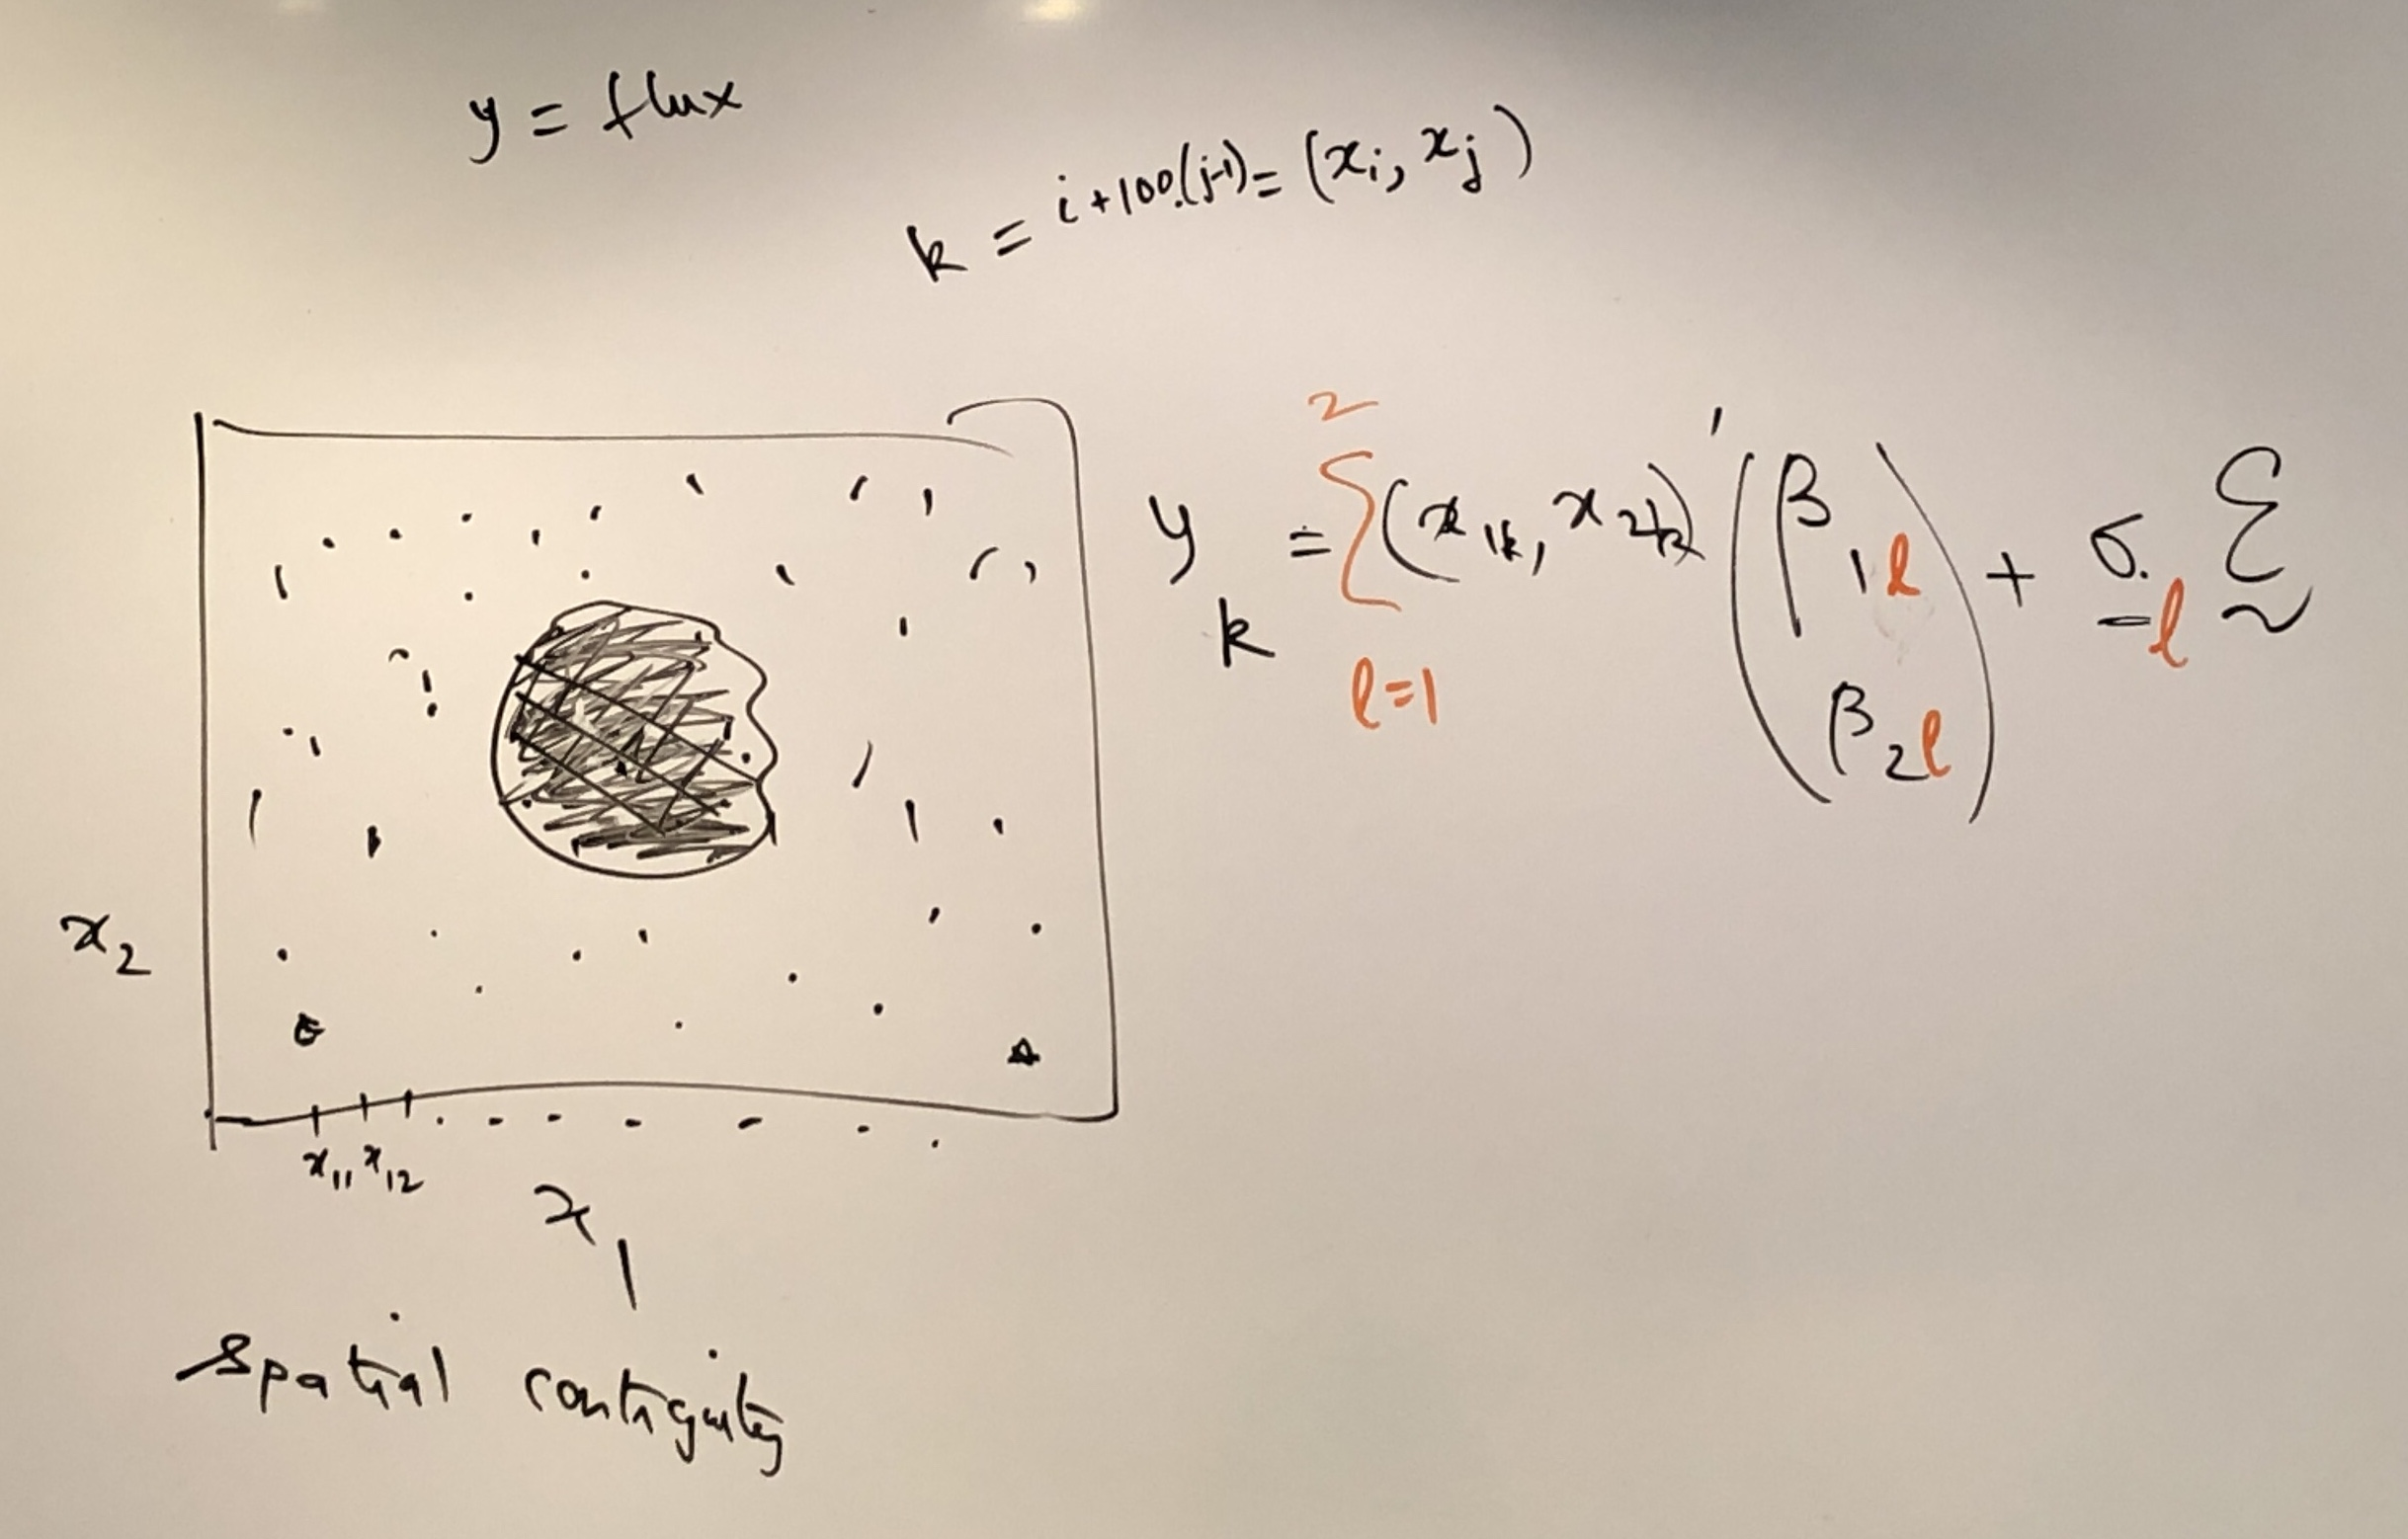
\includegraphics[scale=0.15]{linreg_spatial_mixture_model_2}
\caption{Mixture model example.}
\label{linreg.fig.mix.model.ex}
\end{center}
\end{figure}


\section{Missing observations}

\section{Generalized linear models}\label{linreg.glm}

Exponential family: binomial, Poisson, Beta, negative binomial, etc. See Section \ref{prob.sec.exp.fams} for more information on exponential families. The density is 

\[
g_\eta(y) =  c(y) \exp \left\{  \eta y - \psi(\eta) \right\}
\]


where \(c(y)\) is the \textbf{carrier density}, \(\eta\) is the \textbf{natural parameter}, \(y\) is a \textbf{sufficient statistic}, and \(\psi(\cdot)\) is the \textbf{normalizing function} (or \textbf{cumulant generating function}), chosen so that it is a proper density: that is, choose \(\psi(\eta)\) such that

\[
\int_{\mathbb{R}} g_\eta(y) \ dy = 1,
\]

so

\[
e^{- \psi(y)} = \left( \int_{\mathbb{R}} c(y) e^{\eta y} \ dy \right)^{-1} 
\]

The density is simplest to express in the natural parameter. 

Skewness: third centered moment. 

\[
\frac{\E(Y - \E(Y))^3}{\Var(Y)^{3/2}}
\]

kurtosis: 4th centered moment

\[
\frac{\E(Y - \E(Y))^4}{\Var(Y)}
\]

get excess kurtosis by subtracting 3 (which is Gaussian kurtosis).

In general: cumulant, either centered or raw.

\[
K_\gamma = \E(Y - \E(Y))^\gamma, \qquad K_\gamma = \E(Y^\gamma)
\]

Cumulant generating function:

\[
\psi(\eta) - \psi(\eta_0) = \sum_{\gamma=1}^\infty K_\gamma \frac{(\eta - \eta_0)^r}{r!} 
\]

if you know all the cumulants, you know the distribution exactly.

\begin{enumerate}

\item 

\textbf{Gaussian variables:} Suppose \(y_1, y_2, \ldots y_n\) are i.i.d. \(\mathcal{N}(\mu, 1)\).  

\item

\textbf{Gaussian response:} Suppose \((y_i, x_i)\) are i.i.d. pairs in \(\mathbb{R}^{p + 1}\) with \(y_i \sim \mathcal{N}(x_i' \beta, 1)\). 

\item  \textbf{Exponential family variables:}
Suppose \(Y_1, \ldots, Y_n \) are i.i.d. in an exponential family. Then the density of each is \(g_\eta(y) = e^{\eta y 0 \psi(\eta)} c(y)\) and the joint density is

\begin{equation}\label{linreg.eqn.likelihood}
\prod_{i=1}^n g_\eta(y_i) = \exp \left( \eta \sum_{i=1}^n y_i - n \psi(\eta) \right) \cdot \prod_{i=1}^n c(y_i).
\end{equation}

Then the density of \(\overline{y}\) is simply 

\[
\exp \left\{ n \eta \overline{y} - n \psi(\eta) \right\}
\]

now the natural parameter is \(n \eta\) and the normalizing function is \(n \psi(\eta)\). So

\[
\overline{Y} \sim  \left[ n \deriv{\psi(\eta)}{\eta}, n \deriv{\psi^2(\eta)}{\eta^2} \right].
\]

The log likelihood is the log of (\ref{linreg.eqn.likelihood}):

\[
\log L(\eta) = \ell(\eta) = \sum_{i=1}^n \eta y_i - n \psi(\eta) + \sum_{i=1}^n \log c(y_i).
\]

The maximum likelihood estimate solves

\[
\hat{\eta}_{MLE} := \underset{\eta}{\arg \max} \ell(\eta) 
\]


we have

\[
\deriv{}{\eta} \ell(\eta) = \sum_{i=1}^\eta y_i - n \deriv{}{\eta} \psi(\eta)  , \qquad \deriv{^2}{\eta^2} \ell(\eta) = - n \deriv{^2}{\eta^2} \psi(\eta) = - n \Var(\eta) < 0 
\]

so since this function is concave down it has a unique maximum at 

\[
\sum_{i=1}^n  y_i - n \deriv{}{\eta} \psi(\hat{\eta}_{MLE}) \implies \psi(\hat{\eta}_{MLE})  = \frac{1}{n} \sum_{i=1}^n  y_i = \overline{y} \implies \hat{\mu}_{MLE} = \overline{y}
\]

That is, the MLE of the mean parameter in an exponential family is the sample mean. Due to the equivariance property of the maximum likelihood estimator, the MLE for any function of the mean parameter is simply the function of the MLE for the mean parameter (see Proposition \ref{mathstats.prop.inv.mle}). 

We call the derivative \(\deriv{}{\eta} \ell(\eta) \) the \textbf{score function}. If \(\xi = h(\eta)\), then by the chain rule

\[
\deriv{}{\xi} \ell(\eta) = \left. \deriv{}{\eta} \ell(\eta)  \middle/ \deriv{\xi}{\eta}  \right.
\]

For the mean parameter in particular, we have 

\begin{equation}\label{linreg.mean.param}
\deriv{}{\mu} \ell(\eta) = \left. \deriv{}{\eta} \ell(\eta)  \middle/ \deriv{\mu}{\eta}  \right. =  n (\overline{y} - \mu)/ \Var_\eta (Y)
\end{equation}

(since \(\deriv{}{\eta} \ell(\eta) = n \overline{y} - n \deriv{}{\eta} \psi(\eta)\) and \(\Var_\eta(Y) =\deriv{\mu}{\eta} \)). Also, since the expectation of the score function \(\E(\deriv{}{\eta} \ell(\eta)) = 0\), we hace 

\[
\Var \left( \deriv{}{\eta} \ell(\eta) \right) = \E  \left[ \left( \deriv{}{\eta} \ell(\eta) \right)^2  \right] - \left[ \E \left(  \deriv{}{\eta} \ell(\eta) \right) \right]^2 = \E  \left[ \left( \deriv{}{\eta} \ell(\eta) \right)^2  \right]
\]

We call this the \textbf{Fisher information:}

\begin{equation}\label{linreg.fish.inf}
i_\eta^{(n)} (\xi) := \E  \left[ \left( \deriv{}{\eta} \ell(\eta) \right)^2  \right].
\end{equation}

(See also Definiton \ref{mathstats.def.fish.inf} and Section \ref{mathstats.eff.est} for more on this.) In the case of the mean, we can write this as 

\[
i_\eta^{(n)} (\eta) = \E  \left[ \left( n \overline{y} - n \deriv{}{\eta} \psi(\eta) \right)^2  \right] = \Var \left(n \overline{y} - n \deriv{}{\eta} \psi(\eta) \right) = \Var( n \overline{y}) = n^2 \Var(\overline{y}) = n^2 \Var_\eta(y)/n = n \Var_\eta(y)
\]

 Then substituting (\ref{linreg.mean.param}) into (\ref{linreg.fish.inf}) we have 

\begin{equation}\label{linreg.fish.inf.mean.unb}
i_\eta^{(n)} (\mu) =  \E \left[ \frac{ \left(n \overline{y} - n \deriv{}{\eta} \psi(\eta) \right)^2 }{ \Var_\eta(y) ^2} \right] =  \frac{  \Var \left[ n \overline{y} - n \deriv{}{\eta} \psi(\eta)  \right] }{ \Var_\eta(y) ^2}   = \frac{n \Var_\eta(y)}{\Var_\eta(y)^2} = \frac{n}{\Var_\eta(y)}.
\end{equation}

Note that as \(n\) increases, the Fisher information increases linearly. The Fisher information is inversely proportional to the underlying variance. Again, by Proposition \ref{mathstats.prop.inv.mle}, the plug-in estimator for the Fisher Information using the maximum likelihood estimator for the variance is the MLE for the Fisher information:

\[
\left. i_\eta^{(n)}(\mu) \right|_{\eta = \hat{\eta}_{MLE}} = \frac{n}{\widehat{\Var}_{\eta}(y)} = \E \left[  \left(  \deriv{}{\mu} \ell(\eta) \right) ^2 \right] 
= \left. -  \E \left[   \deriv{^2}{\mu^2} \ell(\eta)  \right] \right|_{\eta = \hat{\eta}_{MLE}} 
\]

In the case of the mean parameter, we can write this as 

\[
=  \left.- \deriv{^2}{\mu^2} \ell(\eta) \right|_{\eta = \hat{\eta}_{MLE}} 
\]

\textbf{Cramer-Rao lower bound} (see Theorem \ref{mathstats.cramer.rao}): 

\[
\Var_\eta(\hat{\xi}) \geq \frac{\left( \deriv{}{\eta} \left[  \E_\eta (\hat{\eta}) \right] \right)^2}{i_\eta^{(n)} (\xi)} 
\]

Any estimator that reaches (or approaches asymptotically) this lower bound is \textbf{(asymptotically) efficient}. Consider an unbiased estimator \(\hat{\xi}\) (\(\E(\hat{\xi} = \xi\)): then the bound reduces to 

\[
\Var_\eta(\hat{\xi}) \geq \frac{1}{i_\eta^{(n)} (\xi)} 
\]

Further, suppose we have an unbiased estimator of the mean parameter \(\hat{\mu}\). Then using (\ref{linreg.fish.inf.mean.unb}) we have

\[
\Var_\eta(\hat{\mu}) \geq \frac{1}{i_\eta^{(n)} (\mu)}  = \frac{\Var_\eta(y)}{n}
\]

Since we saw earlier that the MLE has exactly this variance (\(\Var(\overline{y}) = \Var_\eta(y)/n\)), it is the efficient unbiased estimator for \(\mu\). (However, it turns out that the plug-in MLE estimator for a function of this mean parameter is not in general the efficient unbiased estimator.)

\item \textbf{Exponential family model (GLM):}

We have \(Y_1, \ldots, Y_n\) i.i.d. \(g_\eta\). \(D_n*\eta_1, \eta_2) \)

\end{enumerate}

\subsection{Regression models}

Suppose \(g_\eta = e^{\eta y - \psi(\eta)} \cdot c(y)\), and we observe \(y_i = g_{\eta_i}\), \(i \in [n]\), with \(y_i \indep y_j\) for all \(i \neq j\). Then

\[
g(y_1, \ldots, y_n) = \exp \left\{  \sum_{i=1}^n \eta_i y_i - \psi(\eta_i) \right\} \prod_{i=1}^n c(y_i).
\]

If \(\psi_i  = x_i' \beta \in \mathbb{R}^p\) for some \(\beta\), this is a \textbf{hierarchical model}. In particular, it is an \textbf{exponential family regression model}. We must have that the natural parameter is a linear function of the covariates. If not (\(\eta_i= h(x_i' \beta)\) for some nonlinear \(h\)), we get a \textbf{curved exponential family} and things are more difficult.

\subsection{Applications---Categorical Data}

\begin{enumerate}

\item \textbf{Poisson}

\(\eta_i = \log (\mu_i) = x_i'\beta\). 

\begin{remark}

Recall that for an exponential family, e.g. Poisson, if \(Y \sim \operatorname{Poisson}(\lambda)\), the natural parameter is \(\eta = \log \lambda\) and the mean is \(\lambda\). Then we know that \(\ddot{\psi}(\lambda) = \eta\) \textbf{check, it's something like that} so link function is \(\psi^{-1}\).

\end{remark}

Poisson GLM: no response (logit has response) (going off p.37 of slides ``m3-poisson-glm.pdf") 

choose model with high \(p\)-value (on slide 43) because significance test measures if model fit is significantly worse than saturated model. so if not true, then you want that model.

\item \textbf{Binomial} (logistic, probit). Natural parameter for binomial: \(\log(\pi/(1-\pi))\). Link function:

\[
\log \left( \frac{\pi}{1-\pi} \right) = x_i' \beta.
\] 


\begin{multline*}
\operatorname{logit}(\pi) = \log \left( \frac{\pi}{1-\pi} \right) = \log \left( \frac{\mathbb{P}(Y = 1 \mid X = x_i, Z = z_j) }{\mathbb{P}(Y = 0 \mid X = x_i, Z = z_j) } \right)
\\  = \log \left( \frac{\mathbb{P}(Y = 1 , X = x_i, Z = z_j)/ \mathbb{P}(X = x_i, Z = z_j) }{\mathbb{P}(Y = 0, X = x_i, Z = z_j) / \mathbb{P}(X = x_i, Z = z_j) } \right)  =  \log \left( \frac{\mu_{i 1 k}}{\mu_{i0k}} \right) 
\\  = (\lambda + \lambda_i^x + \lambda_1^y + \lambda_k^z + \lambda_{i1}^{xy} + \lambda_{1k}^{yz} + \lambda_{ik}^{xz}) - 
(\lambda + \lambda_i^x + \lambda_0^y + \lambda_k^z + \lambda_{i0}^{xy} + \lambda_{0k}^{yz} + \lambda_{ik}^{xz}) 
\\ = (\lambda_1^y - \lambda_0^y) + (\lambda_{i1}^{xy} - \lambda_{i0}^{xy}) + (\lambda_{1k}^{yz} - \lambda_{0k}^{yz}) 
\end{multline*}

recall the identifiability constraints: first level is 0. So we can write this as 

\[
=   \lambda_1^y +  \lambda_{i1}^{xy} + \lambda_{1k}^{yz}
\]



If instead \(\pi_i = x_i'\beta\), this is not a natural exponential family. 

Probit model: 

\[
\operatorname{probit}[\pi(x)] = \Phi^{-1}(\pi(x)) = x_i' \beta \qquad \iff \pi(x) = \Phi(x_i'\beta).
\]

\item \textbf{Multinomial}

\end{enumerate}

\subsection{Applications---Continuous Data}

\begin{enumerate}

\item \textbf{Gaussian}: Link function: \(\mu = \E(Y)\).

\item \textbf{Binomial} 

\item \textbf{Multinomial}

\end{enumerate}

\section{Mixed Effects Models}


\(y_{ij}\): \(i\) cluster index, \(i = 1, \ldots n\), \(j\) observation number within each cluster, \(j = 1, \ldots ,d \).

\[
y_{ij} = x_i' \beta + z_{ij} v_i + \sigma \epsilon_{ij}
\]

so \(\beta\) has to do with fixed effects. example: \(i\) is time index, \(j\) is student. so for every user you have universal characteristics for the day \(x_i\) and user-specific measurements \(z_{ij}\). The \(z_{ij}\) effects are called \textbf{random effects}. Hierarchical modeling: suppose \(z_i \in \mathbb{R}^q\) (\(q\) random effects), then we often assume \(u_i\ \sim \mathcal{N}_q(0, \Sigma)\).

Can use with R \texttt{lme4} package.

\section{Miscellaneous Topics}

\subsection{Multinomial Response}

\(c\) categories in \(y\).

\[
\log \left( \frac{\pi_{ij}}{\pi_{ic}} \right) = \operatorname{logit} \left[ \mathbb{P} \left( (y_{ij} = 1 \mid y_{ij} = 1 \text{ or } y_{ic} = 1\right)  \right] = \sum_{k=1}^p x_{ik} \beta_{kj} = x_i' \beta_j.
\]

for \(j = 1, \ldots, c -1\). row \(i\): \((y_{i1}, \ldots, y_{ic})\), \(\sum_{k=1}^c y_{ik} = 1\) probabilities \((\pi_{i1}, \ldots, \pi_{ic})\).

For ordinal random variables: 

\[
\operatorname{logit}( \mathbb{P}(Y_i \leq j) ) =  \log \left[  \frac{\mathbb{P}(Y_i \leq j)}{\mathbb{P}(Y_i > j)} \right]
\]

for example, modeling size S, M, L, XL, XXL to \((1, 2, 3, 4, 5)\). Have a cumulative logit: \(\mathbb{P}(Y_i \leq j)\) is nondecreasing as \(j\) increases. We have

\[
\operatorname{logit}(\mathbb{P}(y_i \leq j)) = \alpha_j + x_i \beta, \qquad i \in \{1, \ldots, n\}, j \in \{1, \ldots, c-1\}
\]

under the monotonicty constraint \(\alpha_1 \leq \alpha_2 \leq \ldots \leq \alpha_{c-1}\). 

\subsection{Zero-inflated response}

Suppose \(y_i = 0\) with probability \(1 - \pi_i\) or has distribution \(f\) with probability \(\pi_i\). That is, \(y_i \sim (1 - \pi_i) \delta_0 + \pi_i f( ;\mu_i)\). Assume \(\operatorname{logit}(\pi_i) = x_i' \beta\), and if \(y_i > 0\), then  \(\log(\mu_i) = w_i' \gamma\) (\(\mu_i\) is mean parameter). For example, \(f\) may be Poisson if \(y\) is discrete or Gaussian if \(y\) is continuous: \(f = \phi(\cdot; \mu, \sigma), f(y) = \phi((y-\mu)/\sigma)\) To estimate: use maximum likelihood.

\[
L(\beta; \gamma, \sigma) = \prod_{i=1}^n (1 - \pi_i)^{I\{y_i = 0\}} \left[ \pi_i \cdot \frac{1}{\sigma} \phi \left(  \frac{y_i - \mu_i}{\sigma} \right) \right]^{I\{Y_i \neq 0\}} 
=  \prod_{i=1}^n \left( \frac{1 - \pi_i}{\pi_i} \right)^{I\{y_i = 0\}} \left[  \frac{1}{\sigma} \phi \left(  \frac{y_i - \mu_i}{\sigma} \right) \right]^{I\{Y_i \neq 0\}} 
\]

note that we can factorize this as a part that depends on \(\beta\) and a part that depends on \(\gamma\) and \(\sigma\). Then log likelihood is 

\[
\underbrace{\sum_{i=1}^n \log \left( \frac{1 - \pi_i}{\pi_i} \right) I\left\{ Y_i = 0  \right\}}_{\ell(\beta)} + \underbrace{\sum_{i=1}^n  \left( - \log(\sigma) - \frac{(y_i - \mu_i)^2}{2 \sigma^2} \right) I\left\{ Y_i \neq 0  \right\}}_{\ell(\gamma, \sigma)}
\]

and 

\[
\ell(\beta) =- \sum_{i: y_i = 0} x_i \beta + \sum_{i=1}^n \log \left( \frac{\exp(x_i' \beta)}{1 + \exp (x_i' \beta)} \right), \qquad \ell(\gamma, \sigma) = - \sum_{i: y_i \neq 0}  \left( \log(\sigma) + \frac{(y_i - \mu_i)^2}{2 \sigma^2} \right) I\left\{ Y_i \neq 0  \right\}
\]

and \(\log(\mu_i) = w_i ' \gamma\).


\subsection{Overdispersion}

\textbf{Exponential Regression Model}


\(y_i \sim g_{\eta_i}\), independent. \(\eta_i = x_i' \beta\), \(\mu_i = \dot{\psi}(\eta_i)\). Likelihood \((L(\eta_i) = \exp(\eta_i y_i - \psi(\eta_i)) \cdot c_0(y_i)\), so (ignoring last part that doesn't depend on \(\eta_i\)) we can write the log likelihood as \(\ell(\eta_i) = \eta_i y_i - \psi(\eta_i)\). 

Estimating equation: maximizing log-likelihood, the first order equations (differentiate with respect to \(\beta\)):

\begin{multline*}
\pderiv{\ell(\beta)}{\beta_j} = 0 , \qquad \forall j \in \{1, \ldots, p\}, \qquad \pderiv{\ell}{\eta_i} = y_i - \dot{\psi}(\eta-i) = y_i - \mu_i
\\ \sum_{i=1}^n \pderiv{\ell_i(\beta)}{\beta_j} = \sum_{i=1}^n \pderiv{\ell_i}{\eta_i} \cdot \pderiv{\eta_i}{\beta_j} = \sum_{i=1}^n (y_i - \mu_i) \cdot x_{ij} = 0 , \qquad j \in\{1, \ldots, p\}.
\end{multline*}

example use: use a quasi-likelihood approach for modeling count data where variance isn't necessarily fixed. Have over-dispersion parameter; in that case, can use different variance for count data.

Example data: Efron data set from 70s on toxoplasmosis. Reasons for overdispersion:

\begin{itemize}

\item subgroups in data

\end{itemize}

Remedies: GLMs in quasi likelihood (``dispersion parameter") or mixed effects/hierarchical/multi-level modeling.

\begin{example}[\textbf{Correlated Binomial Trials}]

\(y_{ij} \sim \operatorname{Bin}(1, \pi_i)\), \(i \in [n], j \in [n_i]\). The correlation between \(y_{ij}\) and \(y_{ik}\) is \(\rho\) for \(j \neq k\); \(|\rho| \leq 1\). We have

\[
y_i = \frac{1}{n_i} \sum_{j=1}^{n_i} y_{ij}
\]

\end{example}

\section{Generalized linear mixed models}

Nature of \(\gamma\) model: something like GARCH, etc. Point is, only a few parameters.

Why is MLE biased? Remember that MLE for \(\sigma^2\) is biased, so basically that's why.

For REML (restricted maximum likelihood): start by projecting \(y\) onto the nullspace of \(X\) so that we don't have to worry about \(\beta\):

\begin{multline*}
y = X \beta+ ZU + \epsilon ,
\\ T := (I - P_X)  = (I - P_X)ZU + (I - P_X) \epsilon = (I - X(X^TX)^{-1}X^T) ZU + (I - X(X^TX)^{-1}X^T)  \epsilon
\end{multline*}

Write down the distribution of \(T\) and the likelihood of \(T\). Turns out log likelihood is

\[
\ell_n( \gamma) = -\frac{1}{2} \left[ (y - X \hat{\beta}_{GLS})^T V^{-1}(\gamma) (y - X \hat{\beta}_{GLS}) + \log \left( |V(\gamma)| \right)   + \log \left( |X^T V(\gamma)X| \right)\right]
\]

where again

\[
\hat{\beta}_{GLS} := (X^T V(\gamma)X)^{-1} X^T (V(\gamma))^{-1} y.
\]

(comes up automatically as a result of projection; not here because of an iterative procedure).

Testing:

\begin{enumerate}

\item \textbf{Fixed effects} (\(\beta\)): Partition \(X = [X_0 | X_1]\), \(\beta = (\beta_0, \beta_1)\). \(H_0: \beta_1 = 0\). Likelihood ratio test:

\[
2 \left[ \underbrace{ \ell(\hat{\beta}, \hat{\sigma}^2; \hat{V})}_{\text{complete model}}  -   \underbrace{\ell(\hat{\beta}_0, \hat{\sigma}_0^2; \hat{V}_0)}_{\text{null model}} \right] \xrightarrow{d} \chi_{\operatorname{dim}(\beta_1)}^2.
\]

Issues: test can be anti-conservative (probability of type 1 error higher than stated \(\alpha\)); asymptotics ``kick in" very late. Parametric bootstrap can work better.

\item \textbf{Random effects} (\(U\)): \(H_0: \sigma_j = 0\) (mean of random effects is 0 by assumption, so if variance is also 0, effect is ``not there"). Also do likelihood ratio test, in the end turns out to also be asymptotically \(\chi^2\). 

\end{enumerate}

Composite effect: both fixed and random effects. (some economic models only allow random effects if there is also a fixed effect---enforce hierarchy). 

\subsection{Longitudinal data analysis and Generalized Estimating Equations}

\(t\) for time, \(i\) for user/customer. \(y_{it}\) has correlation across time. \(\E y_{it} = \mu_{it}\), \(\Var(y_{it}) = \phi a(\mu_{it})\), \(g(\mu_{it} )= X_{it}' \beta + z_{it}' \gamma\) where \(a\) can be any arbitrary function (known variance function). If \(\phi=1\), no overdispersion. Estimate \(\phi\) via quasi-likelihood. This case has no correlation across \(y_{it}\). One way to introduce correlation (and parameterize \(a\)): 

\[
\Var(y_{it}) = \phi A_i^{1/2} R(\alpha) A_i^{1/2}
\]

where \(A_i = \operatorname{diag}(a(\mu_i t))\). For example, for a moving average \(MA(1)\) process, we have

\[
R(\alpha) = \begin{bmatrix}
1 & \alpha & 0 &  \cdots & 0 \\
\alpha & 1 & \alpha &  \cdots & 0 \\
0 & \alpha & 1 & \cdots & 0 \\
\vdots & \vdots & \vdots & \ddots & \vdots \\
0 & 0& 0& \cdots & 1 
\end{bmatrix}
\]

\section{Causal Inference}

\subsection{Factorial Design (see R lab 7)}

2 or more discrete factors. Fully cross-classified.

\[
y_{ijk} = \mu + X \beta + \underbrace{\alpha_i}_{\text{school}} + \underbrace{\beta_j}{\text{class}} + (\alpha \beta)_{ij} + \epsilon_{ijk}
\]

Nested design:

\[
y_{ijk} = \mu + X \beta + \alpha_i + \beta_{ij} + \epsilon_{ijk}.
\]

Imbalanced design:

\[
y_{ijk} = \underbrace{\mu}_{\text{general effect}} + \underbrace{\alpha_i }_{\text{treatement effect}} + \underbrace{\beta_j}_{\text{block effect}} + \epsilon_{ijk}
\]

Complete vs. incomplete design: all treatments do not occur in the same block. Treatment contrast: difference between treatment effect \(i\) and \(j\): \(\alpha_i - \alpha_j\). BIBD: balanced incomplete block designs. All treatment contrasts are estimable. \(I\) treatments, \(J\) blocks. Each treatment occurs exactly \(r\) times in the design. \(n = rI = kJ\). Typically \(r \ll J\) .


\section{Math 547}

Exercise 3.16: this inequality talks about the number of misclassifications, not the probability of misclassification under any distribution.

\subsection{Perceptron Algorithm}

\begin{remark}

Note that the run times only depends on the \(\ell_2\) norm of the solution loadings \(w\) and the \(\ell_2\) norm of the longest vector in the data set. That sounds good since it doesn't depend on the size of the data, but in the worse case \(\theta\) can grow exponentially in the dimension of the data.

Also, note that the actual run time is at least linear in the size of the data, since on each iteration the algorithm checks some multiple of \(m\) points.

\end{remark}

\subsection{Mercer's Theorem}

How is this an infinite-dimensional version of the Exercise? Let \(M\) be a \(k \times k\) real symmetric matrix. By the Spectral Theorem, there exists an orthogonal \(Q\) and a diagonal \(D\) such that \(M = Q^T D Q\). For all \(1 \leq p \leq k\), let \(\lambda_p\) denote the \(p\)th diagonal entry of \(D\). Let \(\psi_i^{p} \in \mathbb{R}^k\) denote the \(i\)th row of \(Q\). Then

\[
m_{ij} = \sum_{p=1}^k \lambda_p \psi_i^{(p)} \psi_j^{(p)}, \qquad \forall 1 \leq i, j \leq k.
\]

Also, \(m(x,y)\) is called a \textbf{kernel.}

How to get \(\psi\) from \(m(x,y)\)? Definte 

\[
\ell_2 := \{ \} 
\]

Note: if we could write the algorithm in terms of \(m(x,y)\), we don't need to specify this embedding \(\phi\) at all. 

\section{Norms}

\begin{proposition}

Let \(C \subseteq \mathbb{R}^n\) be a symmetric (if \(c \in C\) then \(-c \in C\)) convex set containing 0. Define for all \(x \in \mathbb{R}^n\), 

\[
 \lVert x \rVert_C := \inf \left\{  t > 0: \frac{x}{t} \in C \right\}
\]

Then \( \lVert x \rVert_C\) is a norm.

\end{proposition}

\begin{theorem}[\textbf{notes from proof of lemma 6.24}]

\[
d_{2, \mathbb{P}}(f,g)^2 - d_{2, \mathbb{P}_m}(f,g)^2 = ( \E_ \mathbb{P}|f - g|^2) ^{1/2} -  ( \E_ {\mathbb{P}_m}|f - g|^2) ^{1/2} = \E h(X) - \frac{1}{m} \sum_{i=1}^m h(X_i) = \frac{1}{m} \sum_{i=1}^m \left( \E h(X) - h(X_i) \right)
\]

\end{theorem}

note from proof of theorem 6.23: needed to bound number of points in order to apply Sauer-Shelah lemma (only applies for finite number of points)

\begin{definition}[\textbf{Nuclear norm}]\label{statlearning.def.nuc.norm}

Let \(A \in \mathbb{R}^{m_1 \times m_2}\). The \textbf{nuclear norm} of \(A\), denoted \(\lVert A \rVert_*\) is given by

\[
\lVert A \rVert_* := \sum_{j=1}^{\operatorname{rank}(A)} \sigma_j(A), 
\]

where \(\sigma_1(A) \geq \sigma_2(A) \geq \ldots \geq \sigma_{\operatorname{rank}(A)}(A)\) are the singular values of \(A\).

\end{definition}

\begin{definition}[\textbf{Spectral norm} or \textbf{operator norm}]\label{statlearning.def.spec.norm}

Let \(A \in \mathbb{R}^{m_1 \times m_2}\). The \textbf{Spectral norm} or \textbf{operator norm} of \(A\) is given by

\[
\lVert A \rVert := \max_j \sigma_j(A).
\]


\end{definition}

\begin{exercise}\label{statlearning.ex.nuc.norm.op.norm.dual}

Prove that the operator norm is the dual of the nuclear norm. (For any norm \(\lVert \cdot \rVert'\), its dual norm is defined as 

\[
\lVert v \rVert_*' := \sup_{u: \lVert u \rVert' \leq 1 } \langle u, v \rangle.)
\]

That is, prove

\[
\lVert A \rVert = \sup_{\lVert B \rVert_* \leq 1 } \operatorname{Tr}(A^T B).
\]

\end{exercise}

\section{Collaborative Filtering and Trace Regression (Math 541B)}

Notation (Netflix problem): \(m_1\) movies, \(m_2\) users, matrix \(A_0 \in \mathbb{R}^{m_1 \times m_2}\) (rows correspond to movies, columns correspond to users), \(\{A_0\}_{ij} \in [5]\). 

\subsection{Trace Regression}

Let \(A_1, A_2 \in \mathbb{R}^{m_1 \times m_2}\). Define \(\langle A_1, A_2 \rangle := \Tr(A_1^T A_2) = \sum_{i=1}^{m_1} \sum_{j=1}^{m_2} (A_1)_{ij} (A_2)_{ij} \) (equivalent to vectorizing each matrix, then taking inner product). Assume that \((X, Y)\) is a random sample with \(X \in \mathbb{R}^{m_1 \times m_2}, Y \in \mathbb{R}\) such that \(Y = \langle A_0, X \rangle + \xi\) where \(A_0 \in \mathbb{R}^{m_1 \times m_2}\), \(X \in \mathbb{R}^{m_1 \times m_2}\) is a random measurement matrix, and \(\xi \in \mathbb{R}\) is random noise with \(\E \xi =0\), independent of \(X\) by assumption.

\begin{example}

Suppose \(A_0\) and \(X\) are diagonal; that is, \(A_0 = \operatorname{diag}(a_0)\), \(X = \operatorname{diag}(x)\), then \(\langle A_0, X \rangle = \langle a_0, x \rangle = \sum_{j=1}^{m_1} (a_0)_j x_j\). (This is a standard linear model.)

\end{example}

\begin{example}[\textbf{Low-rank matrix completion}]

Suppose \(A_0 \in \mathbb{R}^{m_1 \times m_2}\) has low rank and \(X\) has uniform distribution on the set

\[
\mathcal{E} := \{e_i (m_1) e_j (m_2)^T, i \in [m_1], j \in [m_2]\}
\]

where \(e_i(m) \) has the same dimension as \(m\) and contains \(1\) in the \(i\)th entry and 0 in every other entry. That is, \(e_i (m_1) e_j(m_2)^T\) is a matrix containing a 1 only in entry \((i,j)\) and 0 elsewhere, and 

\[
\langle A_0, e_i(m_1) e_j(m_2)^T \rangle = ( A_0)_{ij}.
\]

(Note that it is important that 

\[
\mathbb{P}(X = e_i e_j^T) > 0 \qquad \forall i , j.
\]

To see why, assume that we only observe movie ratings from one user. Even if that user rates every single movie and \(A_0\) has rank 1, we still will not be able to make any reasonable predictions about the other users' ratings.) So our model is

\[
Y_j = \langle A_0, X_j \rangle + \xi_j, \qquad X_j \sim \operatorname{Uniform}(\mathcal{E}), \qquad \xi_j \indep X_j, \qquad j \in [n].
\]

By Exercise \ref{statlearning.ex.nuc.norm.op.norm.dual}, 

\[
\langle A_1, A_2 \rangle \leq \lVert A_1 \rVert \cdot \lVert A_2 \rVert_*.
\]

(This fact is sometimes known as \textit{trace duality}.) The least squares estimator of \(A_0\) is 

\[
\hat{A} := \underset{S \in \mathbb{R}^{m_1 \times m_2}}{\arg \min} \sum_{j=1}^n (Y_j - \langle S, x_j \rangle )^2.
\]

But since \(n \ll m_1 m_2\), the solution is not unique; this has too many degrees of freedom. (One solution is

\[
\hat{A} = \frac{1}{n} \sum_{j=1}^n Y_j X_j,
\]

but this is not low-rank.) (Exercise: calculate \(\E \lVert \hat{A} - A_0 \rVert_F^2\).)  One idea is to impose a constraint that \(\operatorname{rank}(S) \leq k\). Then the problem becomes

\[
\hat{A} = \begin{aligned}
& \underset{S \in \mathbb{R}^{m_1 \times m_2}}{\arg \min} 
& & \sum_{j=1}^n (Y_j - \langle S, x_j \rangle )^2 \\
& \text{subject to}
& & \operatorname{rank}(S) \leq k , \qquad k \geq \operatorname{rank}(A_0)
\end{aligned}
\]

We know that \(A_0 \in \mathcal{A} = \{A: \operatorname{rank}(A) \leq k, \lVert A \rVert_* \leq \lVert A_0 \rVert_* \}\). But this problem is non-convex. The idea is to replace \(\mathcal{A}\) by its convex hull. Consider the set \(\tilde{\mathcal{A}} \subset \mathcal{A}\) defined by

\[
\tilde{\mathcal{A}} = \left\{ \pm \lVert A_0 \rVert_* = uv^T, u \in \mathbb{R}^{m_1}, v \in \mathbb{R}^{m_2}, \lVert u \rVert_2 = 1, \lVert v \rVert_2 = 1 \right\}.
\]

We claim that the convex hull of \(\tilde{\mathcal{A}}\) is equal to 

\[
\lVert A_0 \rVert_* \cdot B(0, 1, \lVert \cdot \rVert_*)
\]

where

\[
B(0, 1, \lVert \cdot \rVert_*)  = \{S \in \mathbb{R}^{m_1 \times m_2}: \lVert S \rVert_* \leq 1\}.
\]

and is also the convex hull of \(\mathcal{/A}\). Since the set \(\lVert A_0 \rVert_* \cdot B(0, 1, \lVert \cdot \rVert_*)\) contains \(A\) and is convex, the convex hull of \(\mathcal{A}\) is equal to \(\lVert A_0 \rVert_* \cdot B(0, 1, \lVert \cdot \rVert_*\). (We took \(\tilde{\mathcal{A}} \subset \mathcal{A}\) and showed that \(\mathcal{A} \subset \operatorname{co}(\tilde{\mathcal{A}})\). Since \(\tilde{\mathcal{A}} \subset \mathcal{A}\), \(\operatorname{co}(\tilde{\mathcal{A}}) \subseteq \operatorname{co}(\mathcal{A})\), so we must have \(\operatorname{co}(\tilde{\mathcal{A}}) =\operatorname{co}(\mathcal{A})\).)  So we can change our optimization problem to the convex problem

\[
\hat{A} = \begin{aligned}
& \underset{S \in \mathbb{R}^{m_1 \times m_2}}{\arg \min} 
& & \sum_{j=1}^n (Y_j - \langle S, x_j \rangle )^2 \\
& \text{subject to}
& & \lVert S \rVert_* \leq \lVert A_0 \rVert_*.
\end{aligned}
\] 

Lastly, since the nuclear norm of \(A_0\) is unknown, we will replace \( \lVert A_0 \rVert_*\) with a sufficiently large constant:

\[
\hat{A} = \begin{aligned}
& \underset{S \in \mathbb{R}^{m_1 \times m_2}}{\arg \min} 
& & \sum_{j=1}^n (Y_j - \langle S, x_j \rangle )^2 \\
& \text{subject to}
& & \lVert S \rVert_* \leq t
\end{aligned}
\] 

for some \(t > 0\). In practice, we can look at the Lagrangian form:

\[
\hat{A}_\lambda := \underset{S \in \mathbb{R}^{m_1 \times m_2}}{\arg \min} \left\{\sum_{j=1}^n (Y_j - \langle S, x_j \rangle )^2  + \lambda  \lVert S \rVert_*  \right\}
\]

for some \(\lambda \in \mathbb{R}_+\). (Nuclear norm penalization is a convex relaxation.) Consider:

\[
\frac{1}{n} \sum_{j=1}^n (Y_j - \langle S, x_j \rangle )^2  + \lambda  \lVert S \rVert_*
 = \frac{1}{n} \sum_{j=1}^n Y_j^2  + \frac{1}{n} \sum_{j=1}^n \langle S, x_j \rangle ^2  - 2 \left \langle \frac{1}{n} \sum_{i=1}^n X_j Y_j, A \right \rangle + \lambda  \lVert S \rVert_*
\]

Consider the term

\[
 + \frac{1}{n} \sum_{j=1}^n \langle S, x_j \rangle ^2 .
 \]

By the Law of Large Numbers, this converges to its expectation, so we can replace it with its expectation

\[
\E  \langle S, x_j \rangle ^2 = \sum_{i=1}^{m_1} \sum_{j=1}^{m_2} \frac{1}{m_1 m_2} \underbrace{ \langle A_i e_i(m_1) e_j(m_2)  \rangle^2}_{A_{ij}} = \frac{1}{m_1 m_2} \sum_{i,j} A_{ij}^2 = \frac{1}{m_1 m_2} \lVert A \rVert_F^2.
\]

The problem becomes 

\begin{multline*}
\hat{A} = \underset{A}{\arg \min} \left\{ \frac{1}{m_1 m_2} \lVert A \rVert_F^2 - 2   \left \langle \frac{1}{n} \sum_{i=1}^n X_j Y_j, A \right \rangle + \lambda  \lVert S \rVert_* \right\}
\\ = \underset{A}{\arg \min} \left\{ \lVert A \rVert_F^2 - 2   \left \langle \frac{m_ 1 m_2 }{n} \sum_{i=1}^n X_j Y_j, A \right \rangle + \lambda'  \lVert S \rVert_* \right\}
\\ = \underset{A}{\arg \min} \left\{ \lVert \tilde{X} - A \rVert_F^2 + \lambda'  \lVert S \rVert_* \right\}
\end{multline*} 

where 

\[
\tilde{X} := \frac{m_1 m_2}{n} \sum_{j=1}^n Y_j X_j.
\]

Observe that \(\tilde{X}\) is an unbiased estimator of \(A\):

\begin{multline*}
\E \tilde{X} = \frac{m_1 m_2}{n} n \E Y X = m_2 m_2 \E( \langle A_0, X \rangle X + \xi X) =  m_2 m_2 \E( \langle A_0, X \rangle X )
\\   = m_2 m_2 \sum_{i=1}^{m_1} \sum_{j=1}^{m_2} (A_0)_{ij} e_i (m_1) e_j(m_2) = A_0
\end{multline*}

since \(\xi \indep X\) and \(\E \xi = 0\). (So if the penalty is 0, we have an unbiased estimator for \(A_0\), but we want the penalty because the unbiased estimator is bad.)

\begin{theorem}

\(\hat{A}_\lambda\) is given explicitly by the following:

\[
\hat{A}_\lambda = \sum_{j=1}^{\min(m_1, m_2)} \left(  \sigma_j(\tilde{X}) - \frac{\lambda m_1 m_2}{2}  \right)_+ u_i(\tilde{X}) v_j(\tilde{X}) 
\]

where \(x_+ := \max\{0, x\}\) is the soft-thresholding function. (summary: take SVD of \(\tilde{X}\), then apply soft-thresholding to the singular values. soft singular value thresholding.) 

\end{theorem}

\begin{proof}

Consider 

\[
\hat{a}_\lambda = \underset{a \in \mathbb{R}}{\arg \min} \left[ (a - x)^2 + \lambda |a| \right].
\]

Then

\begin{multline*}
0 \in \partial F(\hat{a}_\lambda) \iff \exists v \in \partial | \hat{a}_\lambda|: 2(\hat{a}_\lambda - x) + \lambda v = 0
\\ \partial F(a) = \left\{2(a - x) + \lambda  v, v \in \partial |a| \right\}
%\\ 2 (\hat{a}_\lambda - x) + \lambda v = 0 
\qquad \implies \hat{a}_\lambda = x - \frac{\lambda}{2} v
\end{multline*}

Two possibilities:

\begin{enumerate}[(a)]


\item 

\[
|x| > \frac{\lambda}{2}:
\]

take \(v = \operatorname{sign}(x)\). Then \(\hat{a}_\lambda = (|x| - \lambda/2)  \operatorname{sign}(x)\). 

\item \(|x| \leq \lambda/2\): If \(\hat{a}_\lambda > 0, v = 1\). \(\hat{a}_\lambda = x - \lambda/2 < 0\). If \(\hat{a}_\lambda < 0, v = -1\). Then \(\hat{a}_\lambda = x + \lambda/2 > 0\): contradiction. So \(\hat{a}_\lambda = 0\).  

\end{enumerate}

\( \hat{a}_\lambda = (|x| - \lambda/2)_+ \operatorname{sign}(x)\). 

\end{proof}

Fact: let \(\lVert \cdot \rVert '\) be any norm. Then 

\[
\partial \lVert x \rVert' = \begin{cases}
y: \lVert y \rVert_*' = 1, \langle y, x \rangle = \lVert x \rVert', & x \neq 0, \\
y: \lVert y \rVert_*' \leq 1, & x = 0,
\end{cases}
\]

where \(\lVert \cdot \rVert_*'\) is the dual norm of \(\lVert \cdot \rVert'\). Apply this fact to the nuclear norm to get that 

\[
\partial \lVert A \rVert_* = \left\{  \sum_{j=1}^{\operatorname{rank}(A)} u_j(A) v_j(A)^T + \sum_{j= \operatorname{rank}(A)}^{\min(m_1, m_2)} w_1 u_j(A) v_j(A)^T , \qquad w_j \in [-1, 1] \right\}.
\]

(since singular values are always non-negative, so subdifferntial is 1 when singular value is positive and any element of \([-1,1]\) when singular value is 0.) Let

\[
F(A) := \lVert A - \tilde{X} \rVert_F^2 + \lambda m_1 m_2 \lVert A \rVert_*.
\]

\(A_\lambda\) minimizes \(F(A)\) if and only if \(0 \in \partial F(\hat{A}_\tau)\). Note that 

\[
\partial F(\hat{A}_\lambda) = \left\{ 2(\hat{A}_\lambda - \tilde{X}) + \lambda m_1 m_2 v, \qquad v \in \partial \lVert \hat{A}_\lambda \rVert_* \right\}.
\]

\begin{enumerate}[(a)]

\item

\[
\sigma_j(\tilde{x}) > \frac{\lambda}{2} m_1 m_2 \implies \sigma_j(\hat{A}_\lambda) = \sigma_j(\tilde{x}) - \frac{\lambda}{2} m_1 m_2.
\]

\item

\[
\sigma_j \leq \frac{\lambda}{2} m_2 m_2 \implies \sigma_j(\hat{A}_\lambda) = 0.
\]

\end{enumerate}

Question: which choice of \(w_j\)'s are required here?

\begin{theorem}

Assume that \((X_j, Y_j), j\in [n]\) are i.i.d., \(X_j \sim \operatorname{Uniform}(e)\), \(|Y_j| \leq \eta\) (maximal rating) with probability 1. Let 

\[
M = \frac{1}{n} \sum_{j=1}^n \left(Y_j X_j - \underbrace{\frac{A_0}{m_1 m_2 }}_{\E(Y_j X_j)} \right).
\]

Assume that \(\lambda \geq 2 \lVert M \rVert_1\) (twice the largest singular value of the matrix), and \(n \gg \min\{m_1, m_2\} \log (m_1 + m_2)\) (tells us the number of ratings we have observed exceeds at least the minimal dimension of the matrix by some logarithmic factor; have observed a rating for each movie and each user at least once). Then the following holds:

\[
\lVert \hat{A}_\lambda - A_0 \rVert_F^2 \leq \left( \frac{1 + \sqrt{2}}{2} \right)^2m_1m_2 \lambda^2 \operatorname{rank}(A_0).
\]

(as long as \(\lambda\) is big enough, then estimator performs sufficiently well.)

\end{theorem}

\begin{proposition}

Let 

\[
\lambda \geq 4 \eta \sqrt{\frac{t + \log(m_1 + m_2)}{\min(m_1, m_2)n}}.
\]

Then \(\lambda \geq 2 \lVert M \rVert\) with probability greater than or equal to \(1 - e^{-t}\).

\end{proposition}


With these two results, we get that for

\[
\lambda = 4 \eta \sqrt{\frac{t + \log(m_1 + m_2)}{\min(m_1, m_2)n}},
\]

we get

\begin{multline*}
\lVert \hat{A}_\lambda - A_0 \rVert^2 \leq \underbrace{ \left( \frac{1 + \sqrt{2}}{2} \right)^216}_{\mathbb{C}} \eta^2 m_1m_2 \cdot \frac{t + \log(m_1 + m_2)}{\min(m_1, m_2)n}  \operatorname{rank}(A_0) 
\\ = \frac{\max\{m_1, m_2\} \operatorname{rank}(A_0)}{n} \mathbb{C} \eta^2(t + \log(m))
\end{multline*}

achieves best bound without knowing rank of matrix in advance. 

\end{example}


%
%
%
%
%
%
%
%
%
%

\section{Dynamic Programming}

\subsection{Introduction to Dynamic Programming and Principle of Optimality (Sections 1.1 - 1.3 of \citep{v1_bertsekas2012dynamic} )}

\textbf{Discrete-time dynamic system:}

\begin{enumerate}

\item \textbf{System dynamics:}

\begin{itemize}

\item \(x_k\): state at time \(k\).

\item \(u_k\): control/decision in period \(k\). Policy: mapping between state and action you will take (a policy is a state-dependent decision, not a decision).

\item \(w_k\): random noise. May depend on \(x_k\), \(u_k\), \(k\) itself. But \textbf{conditioned on \(x_k, U_k\)}, we assume \(w_k\) is independent of \(w_{k-1}, \ldots, w_1\).

\end{itemize}

Model: \(x_{k+1} = f_k(x_k, u_k, w_k)\). 

\item \textbf{Additive Cost Structure:}

For period \(k = 0, 1, \ldots, K-1\), cost \(g_k(x_k, u_k, w_k)\) in period \(k\). Then terminal cost \(g_N(x_N)\). Goal: choose a policy to minimize total expected cost

\[
\underset{w_0, \ldots, w_{N-1}}{\E} \left[  \sum_{k=0}^{N-1} g_k(x_k, u_k, w_k) + g_n(x_n)\right].
\]

\end{enumerate}

\begin{example}[\textbf{Inventory control (Example 1.1.1 in \citep{v1_bertsekas2012dynamic} , p.5)l}]\label{stoch.dp.inv.cont.ex}

\begin{enumerate}

\item

Suppose we have a horizon of \(N\) periods. In each period \(k\), \(x_k = \) number of units of the product available to sell. (We allow \(x_k \leq 0\).) \(u_k \geq 0\) is the amount ordered from the supplier in period \(k\). (Assume instantaneous delivery, so zero lead time.) Finally, \(w_k\) would be the demand for the product in period \(k\). We will assume \(w_k \indep w_j\) for all \(k \neq j\). Note that \(x_{k+1} = x_k - w_k + u_k =: f_k(x_k, w_k, u_k)\). 

\item Costs:

\begin{itemize}

\item ordering cost (say \(C \cdot u_k\)).

\item inventory cost: \(i \) per unit per period.

\item Backorder cost: \(b\) per unit per period.

\end{itemize}

So 

\begin{multline*}
g_k(x_k, u_k, w_k) = c u_k + i \cdot \underbrace{x_k^{+}}_{\max\{x_k, 0\}} + b \cdot \underbrace{x_k^{-}}_{\max\{-x_k, 0\}} =  c u_k + i \cdot (x_k + u_k - w_k)^+ + b(w_k - x_k - u_k)^+ 
\\ = c u_k + i (x_{k+1})^+ + b(-x_{k+1})^+.
\end{multline*}

Different notation:

\[
\mathcal{G}(x_k, u_k, w_k) = \underbrace{p}_{\text{backorder cost/period}} \cdot \max\{0, -x\} +  \underbrace{i}_{\text{inventory cost/period}} \cdot \max\{x, 0\},
\]

ordering cost \(c\)/unit, assume \(p > c\) (see Figure \ref{stoch_dp_ic_fig}). 

\begin{figure}[htbp]
\begin{center}
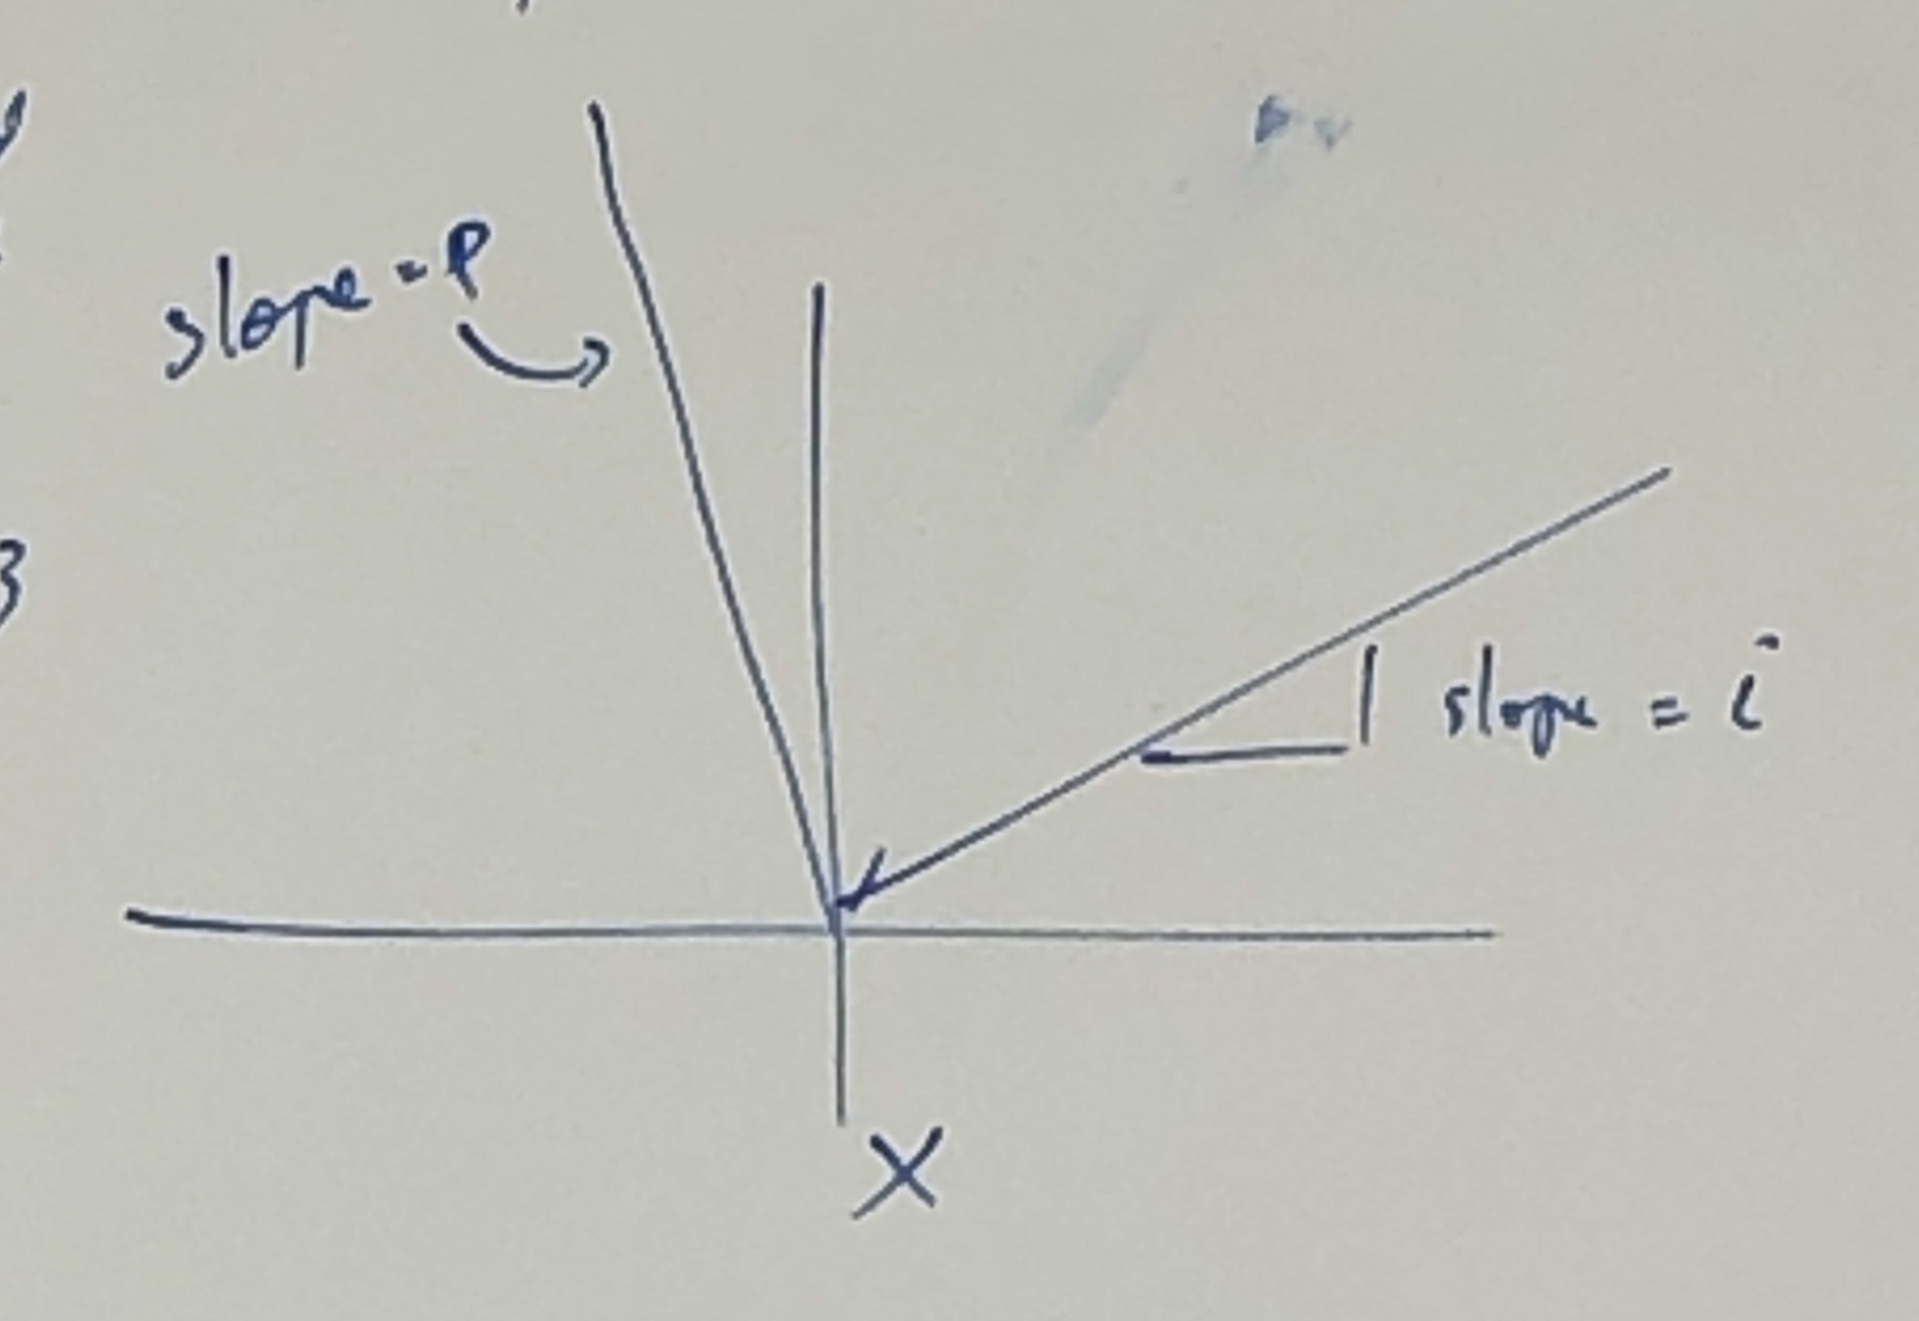
\includegraphics[scale=0.2]{stoch_dp_ic}
\caption{Depiction of cost structure for Example \ref{stoch.dp.inv.cont.ex}. Note that this function \(x \mapsto \mathcal{G}(x)\) is convex in \(x\); this is relevant in the proof of Theorem \ref{stoch.dp.order.up.to.opt}.}
\label{stoch_dp_ic_fig}
\end{center}
\end{figure}


\end{enumerate}

Objective: Minimize

\[
\underset{w_0, \ldots, w_{N-1}}{\E} \left[  \sum_{k=0}^{N-1} g_k(x_k, u_k, w_k) + g_n(x_n)\right].
\]

or

\[
\underset{w_0, \ldots, w_{N-1}}{\E} \left[  \sum_{k=0}^{N-1} c \cdot u_k + \mathcal{G}(x_k + u_k - w_k)\right]  = \underset{w_0, \ldots, w_{N-1}}{\E} \left[  \sum_{k=0}^{N-1} c \cdot u_k + p (w_k -x _k - u_k)^+ + i (x_k + u_k - w_k)^+ \right] .
\]

DP Equation: \(J_k(x_k)\): minimum (over all possible policies) expected cost-to-go given that the state at the beginning of the period is \(x_k\):

\[
J_k(x_k) = \min_{\Pi^k = (\pi_k, \ldots, \pi_{N-1})} \left\{ \underset{w_0, \ldots, w_{N-1}}{\E} \left[  \sum_{\ell=k}^{N-1} c \cdot \pi_\ell(x_\ell) + \mathcal{G}(x_\ell +  \pi_\ell(x_\ell)  - w_\ell)\right]  \right\}.
\]



So, for \(k \in N-1, N-2, \ldots, 0\),

\[
J_k(x_k) = \min_{u_k \geq 0} \left\{ c \cdot u_k + \underset{w_k}{\E} \left[ \mathcal{G}(x_k + u_k - w_k) \right] +  \underset{w_k}{\E}  \left[J_{k+1}(x_k + u_k - w_k ) \right] \right\} .
\]


\end{example}

Open loop policy: Determine \(u_0, u_1, \ldots, u_{N-1}\) in advance. 

\begin{definition}
Closed loop policy: \(u_k\) is a function of the state \(x_k\). 
\end{definition}

In particular, let \(\mu_k: \mathbb{R} \to \mathbb{R}_+\) be our policy. Then \(\mu_k(x_k)\) is the order quantity in period \(k\) given that \(x_k\) units remain. 

\begin{definition}[\textbf{Policy}]

A \textbf{policy} is a sequence of functions 

\[
\pi = \{\mu_0(\cdot), \ldots, \mu_{N-1}(\cdot)\}
\]

mapping the state at state \(k\) to an action. The cost associated with the policy \(\pi\) given an initial state \(x_0\) is denoted by 

\[
J_\pi(x_0) = \E \left[ \sum_{k=0}^{N-1} \left( c \cdot \mu_k(x_k) +  i \cdot (x_k +  \mu_k(x_k) - w_k)^+ + b(w_k - x_k -  \mu_k(x_k))^+ \right) + g_n(x_n) \right].
\]

\end{definition}

Our goal is to find an optimal policy

\[
\pi^* \in \underset{\pi \in \Pi}{\arg \min} \left\{ J_\pi(x_0) \right\} .
\]

Ideally we would like this policy to be uniformly optimal over all possible \(x_0\). (Next week: we'll show that an order-up-to policy is optimal for this problem; that is, for each period \(k\) there exists a constant \(S_k \geq 0\) such that \(\mu_k^*(x_k) = [S_k - x_k]^+\). That is, if the amount of inventory you have is less than \(S_k\), order up to that number; otherwise, don't order.)


\textbf{Basic ingredients:}

\begin{enumerate}[(a)]

\item Discrete-time system: \(x_{k+1} = f_k(x_k, u_k, w_k),\) \(k = 0, 1, \ldots, N-1\).

\item Independent random noise \(w_k\): \(w_k\) can depend on \(x_k, u_k\). 

\item Constraints on control: \(u_k \in \mathcal{U}_k(x_k)\).

\item Additive cost.

\item Closed loop policy.



\end{enumerate}

Note: when the number of states in the system is discrete/finite, instead of writing \(x_{k+1} = f_k(x_k, u_k, w_k)\), you can instead of writing this formula specify transition probabilities, e.g.

\[
\mathbb{P} \left(x_{k+1} = j \mid x_k = i, u_k = u \right) = P_{ij}(u, k)
\]

(i.e. this suffices; all you need is the transition probabilities.)

Note that \(J^*: \mathcal{X} \to \mathbb{R}\) is called an \textbf{optimal value function.} We would like an algorithm to find \(J^*\) (and \(\pi^*\)). Dynamic programming algorithm: the Bellman equations (or DP equations) relies on the principle of optimality.

\begin{definition}[\textbf{Principle of optimality (Section 1.3, p. 20 of \citep{v1_bertsekas2012dynamic} )}]

Suppose \(\pi^* = \{\mu_0^*(\cdot), \ldots, \mu_{N-1}^*(\cdot)\}\) is an optimal policy. Suppose \(\pi^*\) is used, and a given state \(x_i\) occurs in point \(i\) with a positive probability. Consider a sub-problem where we are at \(x_i\) in period \(i\) and wish to minimize the cost-to-go from time \(i\) to the end of the horizon (time \(N\)),

\[
 \E \left[ \sum_{k=i}^{N-1} \left( c \cdot \mu_k(x_k) +  i \cdot (x_k +  \mu_k(x_k) - w_k)^+ + b(w_k - x_k -  \mu_k(x_k))^+ \right) + g_n(x_n) \right].
\]

Then the truncated policy \(\{\mu_i^*(\cdot), \ldots, \mu_{N-1}^*(\cdot)\}\) is also optimal for this sub-problem.

\end{definition}

\begin{example}[Analogy]

Consider the shortest path from LA to New York. If that path passes through Chicago, then the shortest path from Chicago to New York must be identical to that part of the shortest path from LA to New York.

\end{example}

Implications of the principle of optimality: start with a sub-problem of length 0: use the one at the beginning of period \(N\). Then the cost-to-go is \(J_N(x_N) = g_N(x_N)\).

Consider a tail sub-problem of length 1. Suppose we are in state \(x_{N-1}\). Then the optimal policy going forward is

\[
\underset{u_{N-1} \geq 0}{\arg \min} \left\{ c \cdot u_{N-1} + \E \left[   i \cdot (x_{N-1} +  u_{N-1}- w_{N-1} )^+ + b(w_{N-1} - x_{N-1} -  u_{N-1} )^+  + J_N(x_N) \right] \right\}
\]

We can continue backwards:

\[
J_{N-2}(x_{N-2}) = \underset{u_{N-1} \geq 0}{\min} \left\{ c \cdot u_{N-2} + \E \left[   i \cdot (x_{N-2} +  u_{N-2}- w_{N-2} )^+ + b(w_{N-2} - x_{N-2} -  u_{N-2} )^+  + J_{N-1}(x_{N-1}) \right] \right\}
\]

\[
J_{k}(x_{k}) = \underset{u_{k+1} \geq 0}{\min} \left\{ c \cdot u_{k} + \E \left[   i \cdot (x_{k} +  u_{k}- w_{k} )^+ + b(w_{k} - x_{k} -  u_{k} )^+  + J_{k+1}(x_{k+1}) \right] \right\}
\]

and work our way back to \(J_0(x_0)\). 

Sketch of proof: consider the following backward sequence of functions: \(J_N(x_N) = g_N(x_N)\). For \(k = N-1, N-2, \ldots, 2, 1, 0\), 

\begin{equation}\label{stoch.dp.1}
J_{k}(x_{k}) =  \underset{u_{k} \in \mathcal{U}_k(x_k)}{\min} \left\{  \E\left[ g_k(x_k, u_k, w_k) + J_{k+1} \left (f_k(x_k, u_k, w_k) \right)\right] \right\}
\end{equation}

\begin{theorem}[\textbf{Optimality of Dynamic Programming Algorithm (Proposition 1.3.1 in \citep{v1_bertsekas2012dynamic}, p. 25)}]

For every initial state \(x_0\), the optimal cost \(J^*(x_0)\) is equal to \(J_0(x_0)\). Moreover, if \(\mu_k^* = \mu_k^*(x_k)\) minimizes the right hand side of (\ref{stoch.dp.1}), then \(\pi^* =  \{\mu_0^*(\cdot), \ldots, \mu_{N-1}^*(\cdot)\}\) is an optimal policy.

\end{theorem}

Note: \(\mu_k^*\) is a function that maps the state at time \(k\) to an action. \(u_k\) is that action.

\begin{proof}

For any admissible policy \(\pi = \{ \mu_0(\cdot), \ldots, \mu_{N-1}(\cdot)\}\), let \(\pi^k =  \{ \mu_k(\cdot), \ldots, \mu_{N-1}(\cdot)\}\) for the tail subproblem of length \(N-k\) (starting from period \(k\)). For \(k = 0, 1, \ldots, N-1\), let \(J_k^*(x_k)\) be the minimum cost-to-go for the \(N-k\) stage problem given that we are in state \(x_k\) at time \(k\). That is,

\[
J_k^*(x_k) = \min_{\pi^k =  \{ \mu_k(\cdot), \ldots, \mu_{N-1}(\cdot)\}}  \left\{ \E \left[ \sum_{i=k}^{N-1}g_i(x_i, \mu(x_i), w_i) + g_N(x_N) \right] \right\}
\]

where \(g_i(x_i, \mu(x_i), w_i) =  \left( c \cdot \mu_i(x_i) +  i \cdot (x_i +  \mu_i(x_i) - w_i)^+ + b(w_i - x_i -  \mu_i(x_i))^+ \right) \). (Note: \(J_0^*(x_0) = J^*(x_0)\). We'll prove by induction that \(J_k^*(x_k) = J_k(x_k)\) for all \(k = N, N-1, \ldots, 2, 1, 0\). 

\textbf{Base case:} is it true that \(J_N^*(x_N) = J_N(x_N)\)? Yes; just have to minimize \(g_N(x_N)\). 

\textbf{Inductive step:} Suppose \(J_{k+1}^*(x_{k+1}) = J_{k+1}(x_{k+1})\) for all \(x_{k+1}\). We'll now show that \(J_{k}^*(x_{k}) = J_{k}(x_{k})\) for all \(x_k\). Note that 

\begin{multline*}
J_k^*(x_k) = \min_{(\mu_k(\cdot), \pi^{k+1})}  \left\{ \E \left[ g_k(x_k, \mu(x_k), w_k) +  \sum_{i=k+1}^{N-1}g_i(x_i, \mu(x_i), w_i)  + g_N(x_N) \right] \right\}
\\ = \min_{\mu_k(\cdot)}   \left\{ \E \left[ g_k(x_k, \mu(x_k), w_k) \right] +  \min_{ \pi^{k+1}}\left\{\E \left[ \sum_{i=k+1}^{N-1}g_i(x_i, \mu(x_i), w_i)  + g_N(x_N)  \right] \right\} \right\}
\\ = \text{(by definition) } \min_{\mu_k(\cdot)}   \left\{ \E \left[ g_k(x_k, \mu(x_k), w_k) \right] +  J_{k+1}^*(x_{k+1}) \right\} 
\\ = \text{(by inductive hypothesis) } \min_{\mu_k(\cdot)}   \left\{ \E \left[ g_k(x_k, \mu(x_k), w_k) \right] +  J_{k+1}(x_{k+1}) \right\} 
\\ = \underset{u_{k} \in \mathcal{U}_k(x_k)}{\min}  \left\{ \E \left[ g_k(x_k, \mu(x_k), w_k) \right] +  J_{k+1}(f_k(x_k, \mu_k(x_k), w_k)) \right\} ,
\end{multline*}

verifying that (\ref{stoch.dp.1}) is the minimal cost.

\end{proof}

\subsection{State Augmentation and Other Reformulations (Section 1.4 of \citep{v1_bertsekas2012dynamic})}

%Forms of \(x_{k+1} = f_k(x_k, u_k, w_k)\):

\begin{itemize}

\item \textbf{Time lag:} Suppose that \(x_{k=1}\) depends on \(x_k, u_k\), and \(x_{k-1}, w_{k-1}\). Then \(x_{k+1} = f(x_k, u_k, w_k, x_{k-1}, w_{k-1})\). Trick: augment the state variable: \(\tilde{x_k} = (x_k, x_{k-1}, w_{k-1})\). Then \(\tilde{x}_{k+1} = \tilde{f}(\tilde{x}_k, u_k, w_k)\); in particular,

\[
\begin{pmatrix}
x_{k+1} \\
x_k \\
w_{k-1}
\end{pmatrix} = \begin{pmatrix}
 f(x_k, u_k, w_k, x_{k-1}, w_{k-1}) \\
x_k \\
w_{k-1}
\end{pmatrix} 
\]

\item \textbf{Forecast:} Suppose at time \(k\) we observe a forecast \(y_k\) that influences our assessment of the probability distribution of \(w_k\). In particular, suppose \(w_k\) can have one of \(m\) possible distributions \(Q_1(\cdot), \ldots, Q_m(\cdot)\). Then the forecast is \(y_k \in \{1, \ldots, m\}\). Assume \(y_k\) is exogenous. Suppose we have a random variable \(\xi_k\) such that if \(\xi_k = i\), then \(w_{k+1}\) occurs according to probability distribution \(Q_i\), and \(\mathbb{P}(\xi_k = i) = p_i\). The state at time \(k\) is then \(\tilde{x}_k = (x_k, y_k)\), and

\[
\tilde{x}_{k+1} = \begin{pmatrix}
x_k \\
y_{k+1}
\end{pmatrix} = \begin{pmatrix}
f_k(x_k, u_k, w_k) \\
\xi_k
\end{pmatrix} = \tilde{f}_k((x_k, y_k); u_k, w_k).
\]

Then

\[
J_k(x_k, y_k) = \underset{u_k \in \mathcal{U}_k}{\min} \underset{w_i \sim Q(\cdot)}{\E} \left[ g_k(x_k, y_k, w_k) + \underbrace{\sum_{j=1}^m \mathbb{P}(\xi_{k+1} = j) \cdot J_{k+1}(x_{k+1}, j)}_{\text{expected cost-to-go}}\right].
\]

\item \textbf{Correlated disturbances:} \(w_k = \lambda w_{k-1} + \xi_k\), where \(\xi_0, \ldots, \xi_{N-1}\) are i.i.d. Then (letting \(y_k = w_{k-1}\))

\[
\begin{pmatrix}
x_{k+1} \\
y_{k+1}
\end{pmatrix} = \begin{pmatrix}
f_k((x_k, w_k); u_k, \lambda w_{k-1} + \xi-k) \\
\lambda y_k + \xi_k
\end{pmatrix}
\]

\item \textbf{Removal of uncontrollable states:} Suppose the state is described by \((x_k, y_k)\), where \(x_{k+1} = f_k((x_k, y_k), u_k, w_k)\) and the evolution of \(y_k\) is generated by \(\mathbb{P}_k(y_k \mid x_k)\) and is independent of the control (except from the state \(x_k\)). Standard dynamic program:

\[
J_k(x-k, y-k) = \min_{u \in \mathcal{U}_k} \E \left[  g_k(x_k, y_k, u_k, w_k) + \E \left(  f_k(x_k, y_k, u_k, w_k) \right) \right]
\]

We would like to reduce the dimension of the state space since \(y_k\) is dependent on \(x_k\) (and a probability distribution). One way to do this is as follows: 

\[
\hat{J}_k(x_k) = \E_{y_k} \left[ J_k(x_{k+1}, y_{k+1}) \mid x_k \right] = \sum_a \mathbb{P}(y_{k+1} = a \mid x_k) \cdot J_k(x_k, a).
\]

Question: how is \(\hat{J}_k(\cdot)\) related to \(\hat{J}_{k+1}(\cdot)\)?

\begin{multline*}
\hat{J}_h(x_h) = \E_{y_h}  \left[ J_h(x_h, y_h) \mid x_h \right] 
\\ = \E_{y_h} \left[  \min_{u_k} \left\{ \E_{w_h, x_{k=1}, y_{k+1}} \left( g_k(x_k, y-k, u_k, w_k) + J_{k+1}(x_{k+1}, y_{k+1}) \mid x_k, y_k, u_k \right) \right\} \mid x_h \right] 
\\ = \E_{y_h} \left[  \min_{u_k} \left\{ \E_{w_h, x_{k=1}} \left( g_k(x_k, y-k, u_k, w_k) + \E \left[ J_{k+1}(x_{k+1}, y_{k+1}) \mid x_k, y_k, w_k \right] \mid x_k, y_k, u_k \right) \right\} \mid x_h \right] 
\\ = \E_{y_h} \left[  \min_{u_k} \left\{ \E_{w_h, x_{k=1}} \left( g_k(x_k, y-k, u_k, w_k) + \hat{J}_{k+1}(f_k(x_k, y_k, u_k, w_k) \mid x_k, y_k, u_k \right) \right\} \mid x_h \right] 
\end{multline*}

\end{itemize}

\subsection{Inventory Control (Section 3.2 of \citet{v1_bertsekas2012dynamic} )}

See Example \ref{stoch.dp.inv.cont.ex} for setup.

\begin{theorem}[\textbf{Order-up-to Polices Are Optimal}]\label{stoch.dp.order.up.to.opt}

For each period \(k\), there exists a threshold \(S_k \geq 0\) such that 

\[
\mu_k^*(x_k) = [S_k - x_k]^+  = \begin{cases}
S_k - x_k, & x_k \leq S_k, \\
0, & \text{otherwise.}
\end{cases}
\]

\end{theorem}

\begin{proof} 

The DP algorithm is as follows:

\begin{align*}
J_N(x_N) & = 0,
\\ J_k(x_k) & = \min_{u_k \geq 0} \left\{ c \cdot u_k + \underset{w_k}{\E} \left[ \mathcal{G}(x_k + u_k - w_k)  + J_{k+1}(x_k + u_k - w_k ) \right] \right\} 
%\\  & = \min_{u_k \geq 0} \left\{ c \cdot u_k + \underset{w_k}{\E} \left[ \mathcal{G}(x_k + u_k - w_k)  + J_{k+1}(x_k + u_k - w_k ) \right] \right\} 
%\\ & = \min_{u_k \geq 0} \left\{ c u_k + H(x_k + u_k) + \E \left[ J_{k+1}(x_k + u_k - w_k)\right] \right\}
\end{align*}

where again

\[
\mathcal{G}(x_k +  u_k -  w_k) := \underbrace{p}_{\text{backorder cost/period}} \cdot \max\{0, w_k - x_k - u_k\} +  \underbrace{i}_{\text{inventory cost/period}} \cdot \max\{x_k + u_k - w_k, 0\},
\]

Note that \(\mathcal{G}\) depends on \(k\) whenever the probability distribution of \(w_k\) depends on \(k\), but we will assume all demands are identically distributed for simplicity (even though the analysis carries through easily if the distribution of demand is time-varying).



%where the function \(H\) is defined by \(H(y) := \E \left[ r(y - w_k) \right] = p \E \left[ \max\{0, w_k - y\} \right] + h \E \left[\max\{0, y -  w_k \} \right]\).


Now we will prove a lemma.

\begin{lemma}

\(J_k(\cdot)\) is convex.

\end{lemma}

\begin{proof}

We will prove the result by induction. The base case is trivially true because \(J_N(\cdot) = 0\) (note that we could replace \(J_N(\cdot)\) with any convex function and the rest of the proof would follow). Assume \(J_{k+1}(\cdot)\) is convex. Recall from Example \ref{stoch.dp.inv.cont.ex}

\begin{align}
J_k(x_k) & = \min_{u_k \geq 0} \left\{ c \cdot u_k + \underset{w_k}{\E} \left[ \mathcal{G}(\underbrace{x_k + u_k}_{y_k} - w_k)  + J_{k+1}(x_k + u_k - w_k ) \right] \right\} \nonumber \\
& = \min_{y_k \geq x_k} \left\{ c \cdot (y_k - x_k) + \underset{w_k}{\E} \left[ \mathcal{G}(y_k - w_k)  + J_{k+1}(y_k - w_k ) \right] \right\} \nonumber \\
& = -c x_k +  \min_{y \geq x_k} \left\{ c  y  + \underset{w_k}{\E} \left[ \mathcal{G}(y - w_k)  + J_{k+1}(y - w_k ) \right] \right\} \nonumber \\
& = -c x_k +  \min_{y \geq x_k} \left\{ G_k(y) \right\} \label{inv.cont.ctg}
\end{align}

where we let \(G_k(y) := cy + \underset{w_k}{\E}[ \mathcal{G}(y - w_k) + J_{k+1}(y - w_k)]  \). We claim that \(G_k(y)\) is convex in \(y\) by the following argument. First, note that \(\mathcal{G}(x) := p \cdot \max\{0, -x\} + i \max\{x, 0\}\) is convex in \(x\). Therefore \(\underset{w_k}{\E}[\mathcal{G}(y - w_k)]\) is convex in \(y\) since it is convex for each \(w_k\) and taking expectations preserves convexity. 

Next, for each realized value of \(w_k = \overline{w}_k\), \(y \mapsto \mathcal{G}(y - \overline{w}_k) + J_{k+1}(y - \overline{w}_k)\) is convex because \(J_{k+1}\) is a convex function of an affine function and likewise with \(\mathcal{G}(y - \overline{w}_k)\) (see Figure \ref{stoch_dp_ic_fig}). Therefore the result follows when you take expectations.

We will briefly take a detour to consider the end behavior of \(G_k(\cdot)\). As \(y \to \infty\), we know that \(cy \to \infty\). We know that \(\mathcal{G}(\cdot)\) is always nonnegative and likewise with \(J_{k+1}(y - w_k)\), so we must have that as \(y \to \infty\), \(G_k(\cdot) \to \infty\). As \(y \to -\infty\), because of the assumption that \(p > c\) (and that \(J_{k+1}\) is convex), we have that \(G_k(y) \to \infty\). Therefore since \(G_k(\cdot)\) is continuous, a minimizer of \(G_k(\cdot)\) exists. 

Let \(S_k\) be a minimizer of \(G_k(\cdot)\). Note that if \(x_k \geq S_k\), then \(\min_{y \geq x_k} G_k(y) = G_k(x_k)\) due to the convexity of \(G_k(\cdot)\). Clearly if \(x_k \leq S_k\), then \(\min_{y \geq x_k} G_k(y) = G_k(S_k)\). (Note that if \(S_k\) is not the only minimizer, this still holds.) In summary, we have

\begin{equation}\label{dp.inventory.control.cvx.fcn}
J_k(x_k) = \begin{cases}
-c x_k +  G_k(S_k)  & x_k \leq S_k ,\\
-c x_k +  G_k(x_k)  & x_k > S_k .\\
\end{cases}
\end{equation}

\begin{figure}[htbp]
\begin{center}
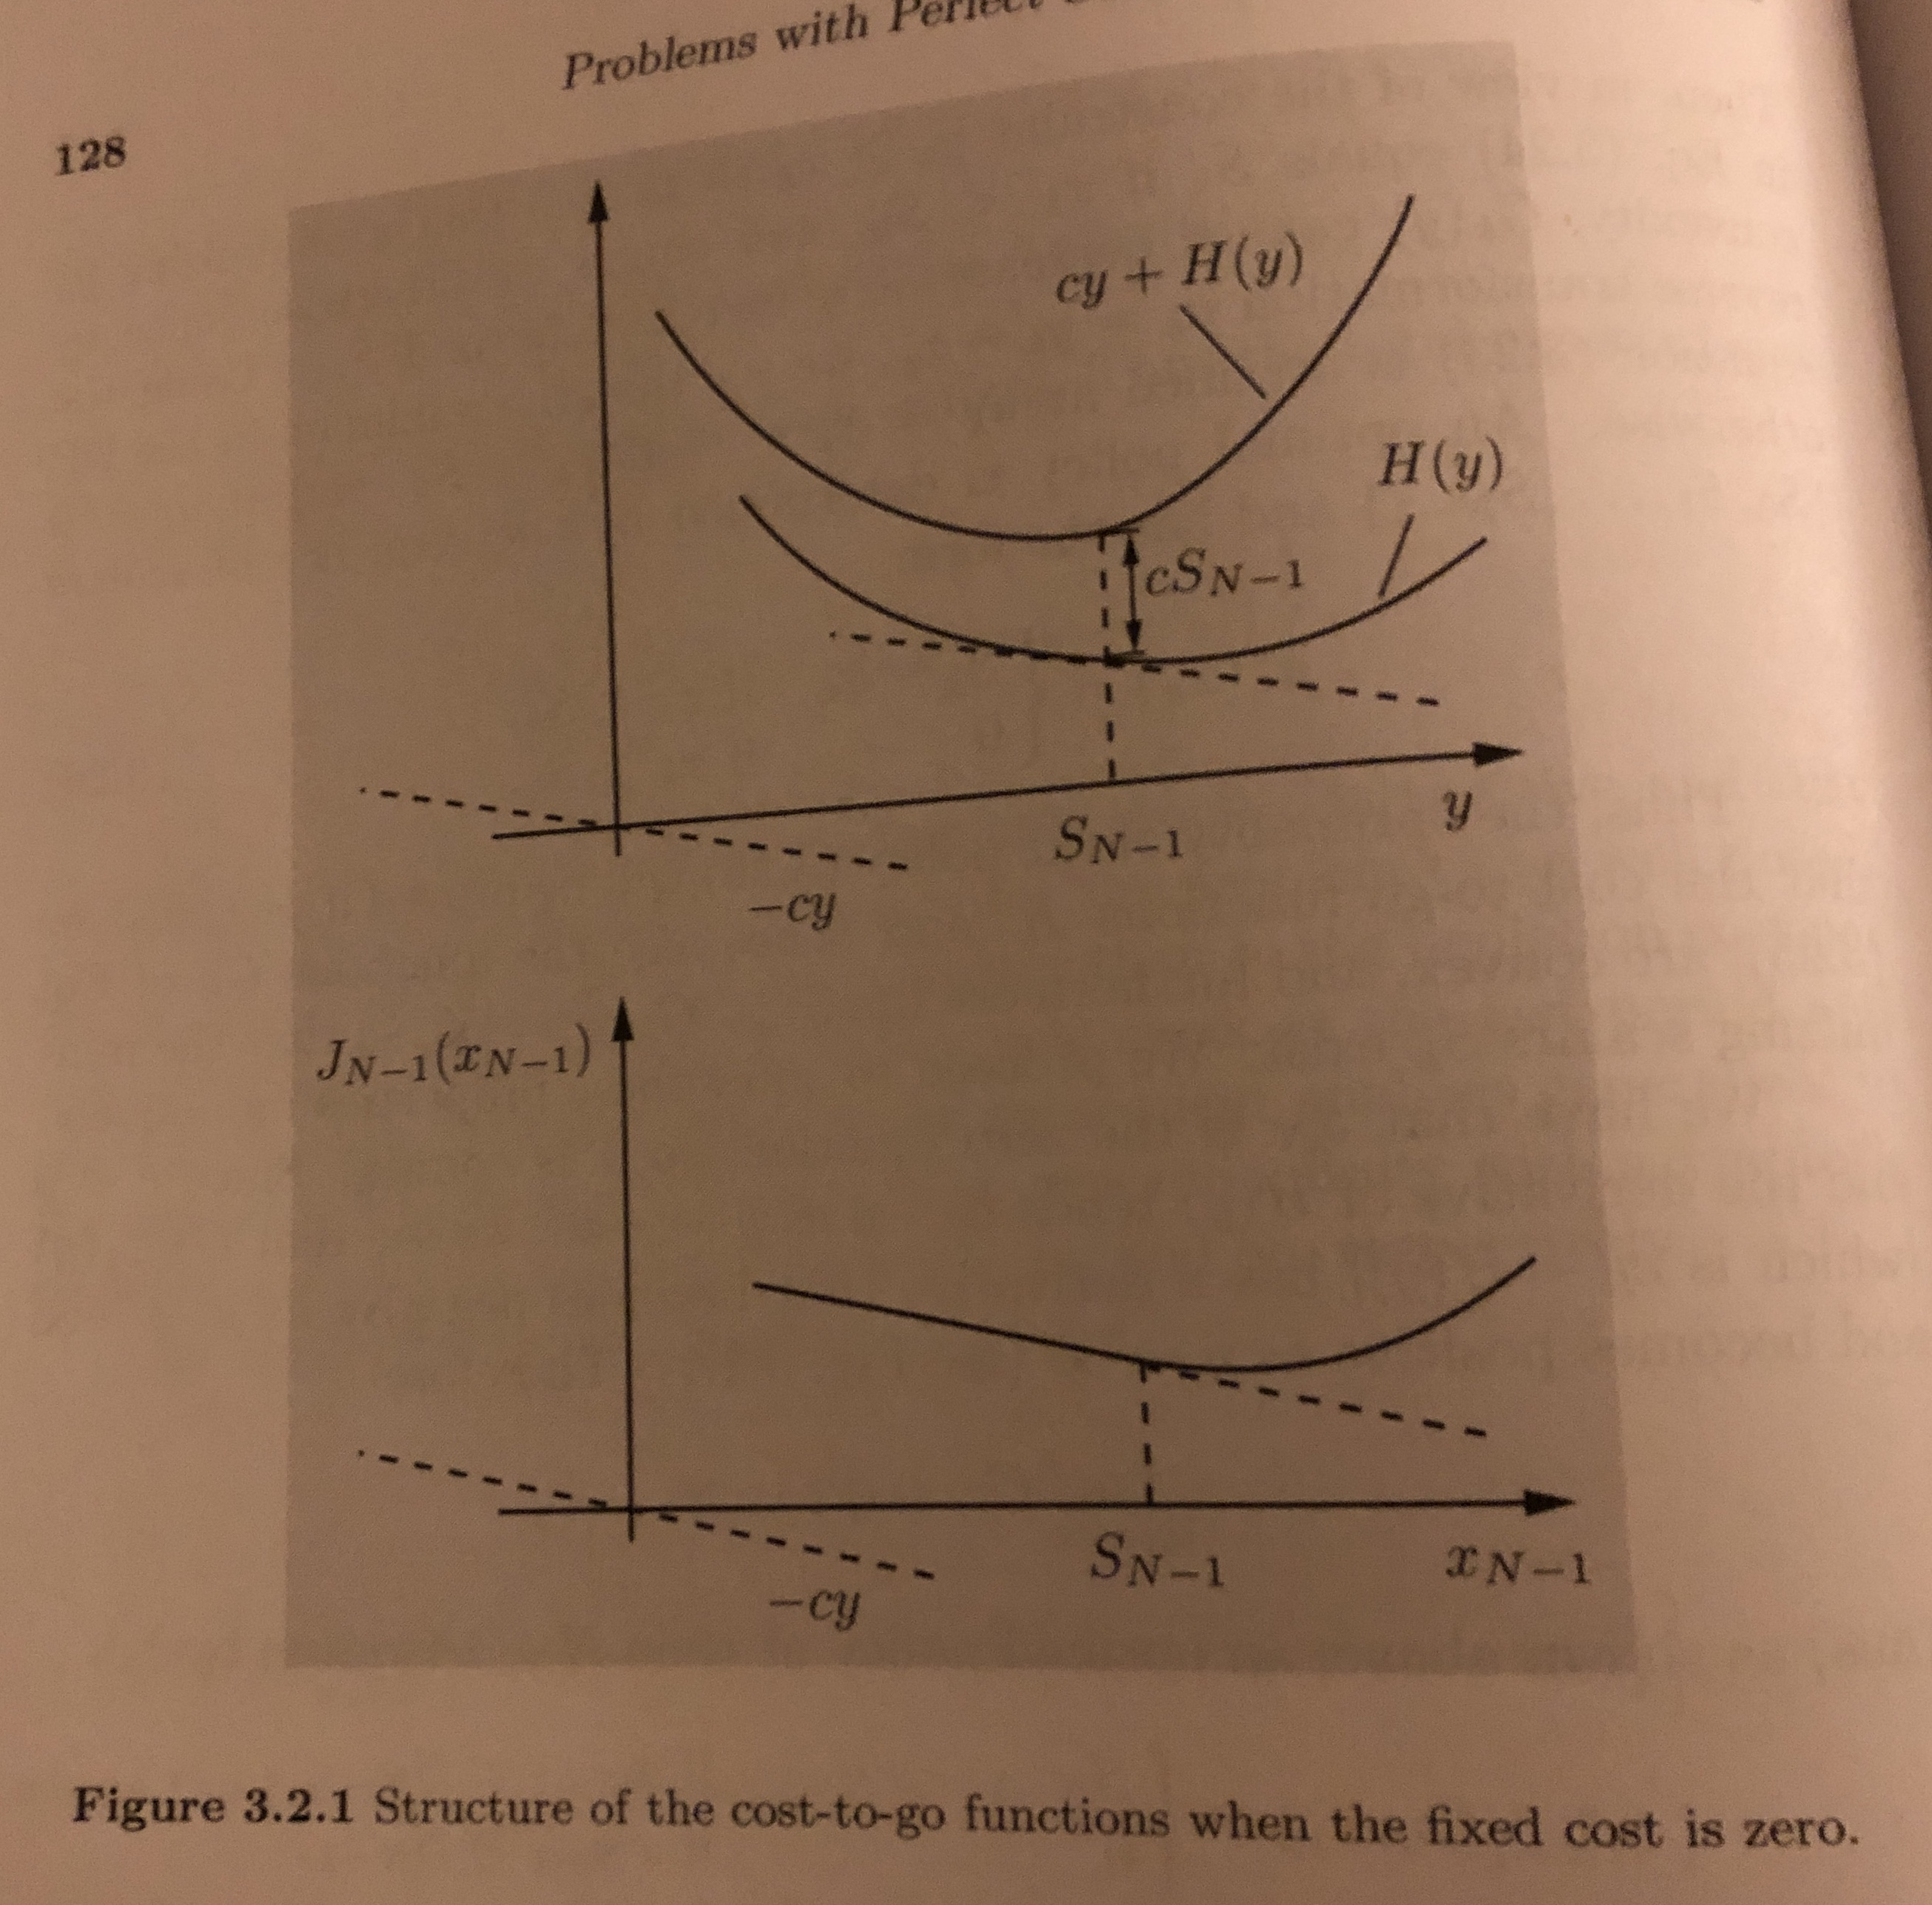
\includegraphics[scale=0.15]{dp_inventory_control}
\caption{Cost-to-go function for inventory control problem. (The notation from \citet{v1_bertsekas2012dynamic} differs slightly from ours, but the lower figure shows that the cost-to-go is linear to the left of the minimizer and convex and nondecreasing to the right of the minimizer, as shown in Equation (\ref{dp.inventory.control.cvx.fcn})).}
\label{dp_inventory_control_fig}
\end{center}
\end{figure}


Each of these functions is continuous and convex in \(y\). Therefore \(J_k(x_k) = -c x_k + \min_{y \geq x_k} G_k(y)\) is convex in \(x_k\). (See Figure \ref{dp_inventory_control_fig}.)

\end{proof}


We have shown that a minimizer for \(G_k\) is given by \(S_k\) if \(x_k < S_k\) and \(x_k\) otherwise. Then since \(u_k = y_k - x_k\) in (\ref{inv.cont.ctg}), a minimizer for (\ref{inv.cont.ctg}) is attained at \(u_k = S_k - x_k\) if \(x_k < S_k\), and at \(u_k = 0\) otherwise. 

\end{proof}

Next we will consider fixed orders cost. Before we find the optimal policy in this case, we will define some terms and derive some results we will need.

\begin{definition}[\textbf{\(K\)-convexity; Definition 3.2.1 in Section 3.2 of \citet{v1_bertsekas2012dynamic}, p. 130}]\label{stoch.dp.k.cvx}

A real-valued function \(g\) is \(K\)\textbf{-convex} for \(K \geq 0\) if 

\begin{equation}\label{dp.k.cvx.defn}
K + g(z+y) \geq g(y) + z \left( \frac{ g(y) - g(y-b)}{b} \right)
\end{equation}

for all \(z \geq 0\), \(b >0\), and all \(y \in \mathbb{R}\). Equivalent: for all \(x < y < z'\), 

\begin{equation}\label{stoch.dp.k.cvx.2}
K + g(z') \geq g(y) + (z'-y) \left(  \frac{g(y) - g(x)}{y - x} \right).
\end{equation}

(This construction follows from (\ref{dp.k.cvx.defn}) by setting \(x := y-b < y\) and \(z' := z + y \geq y\).)

\begin{figure}[htbp]
\begin{center}
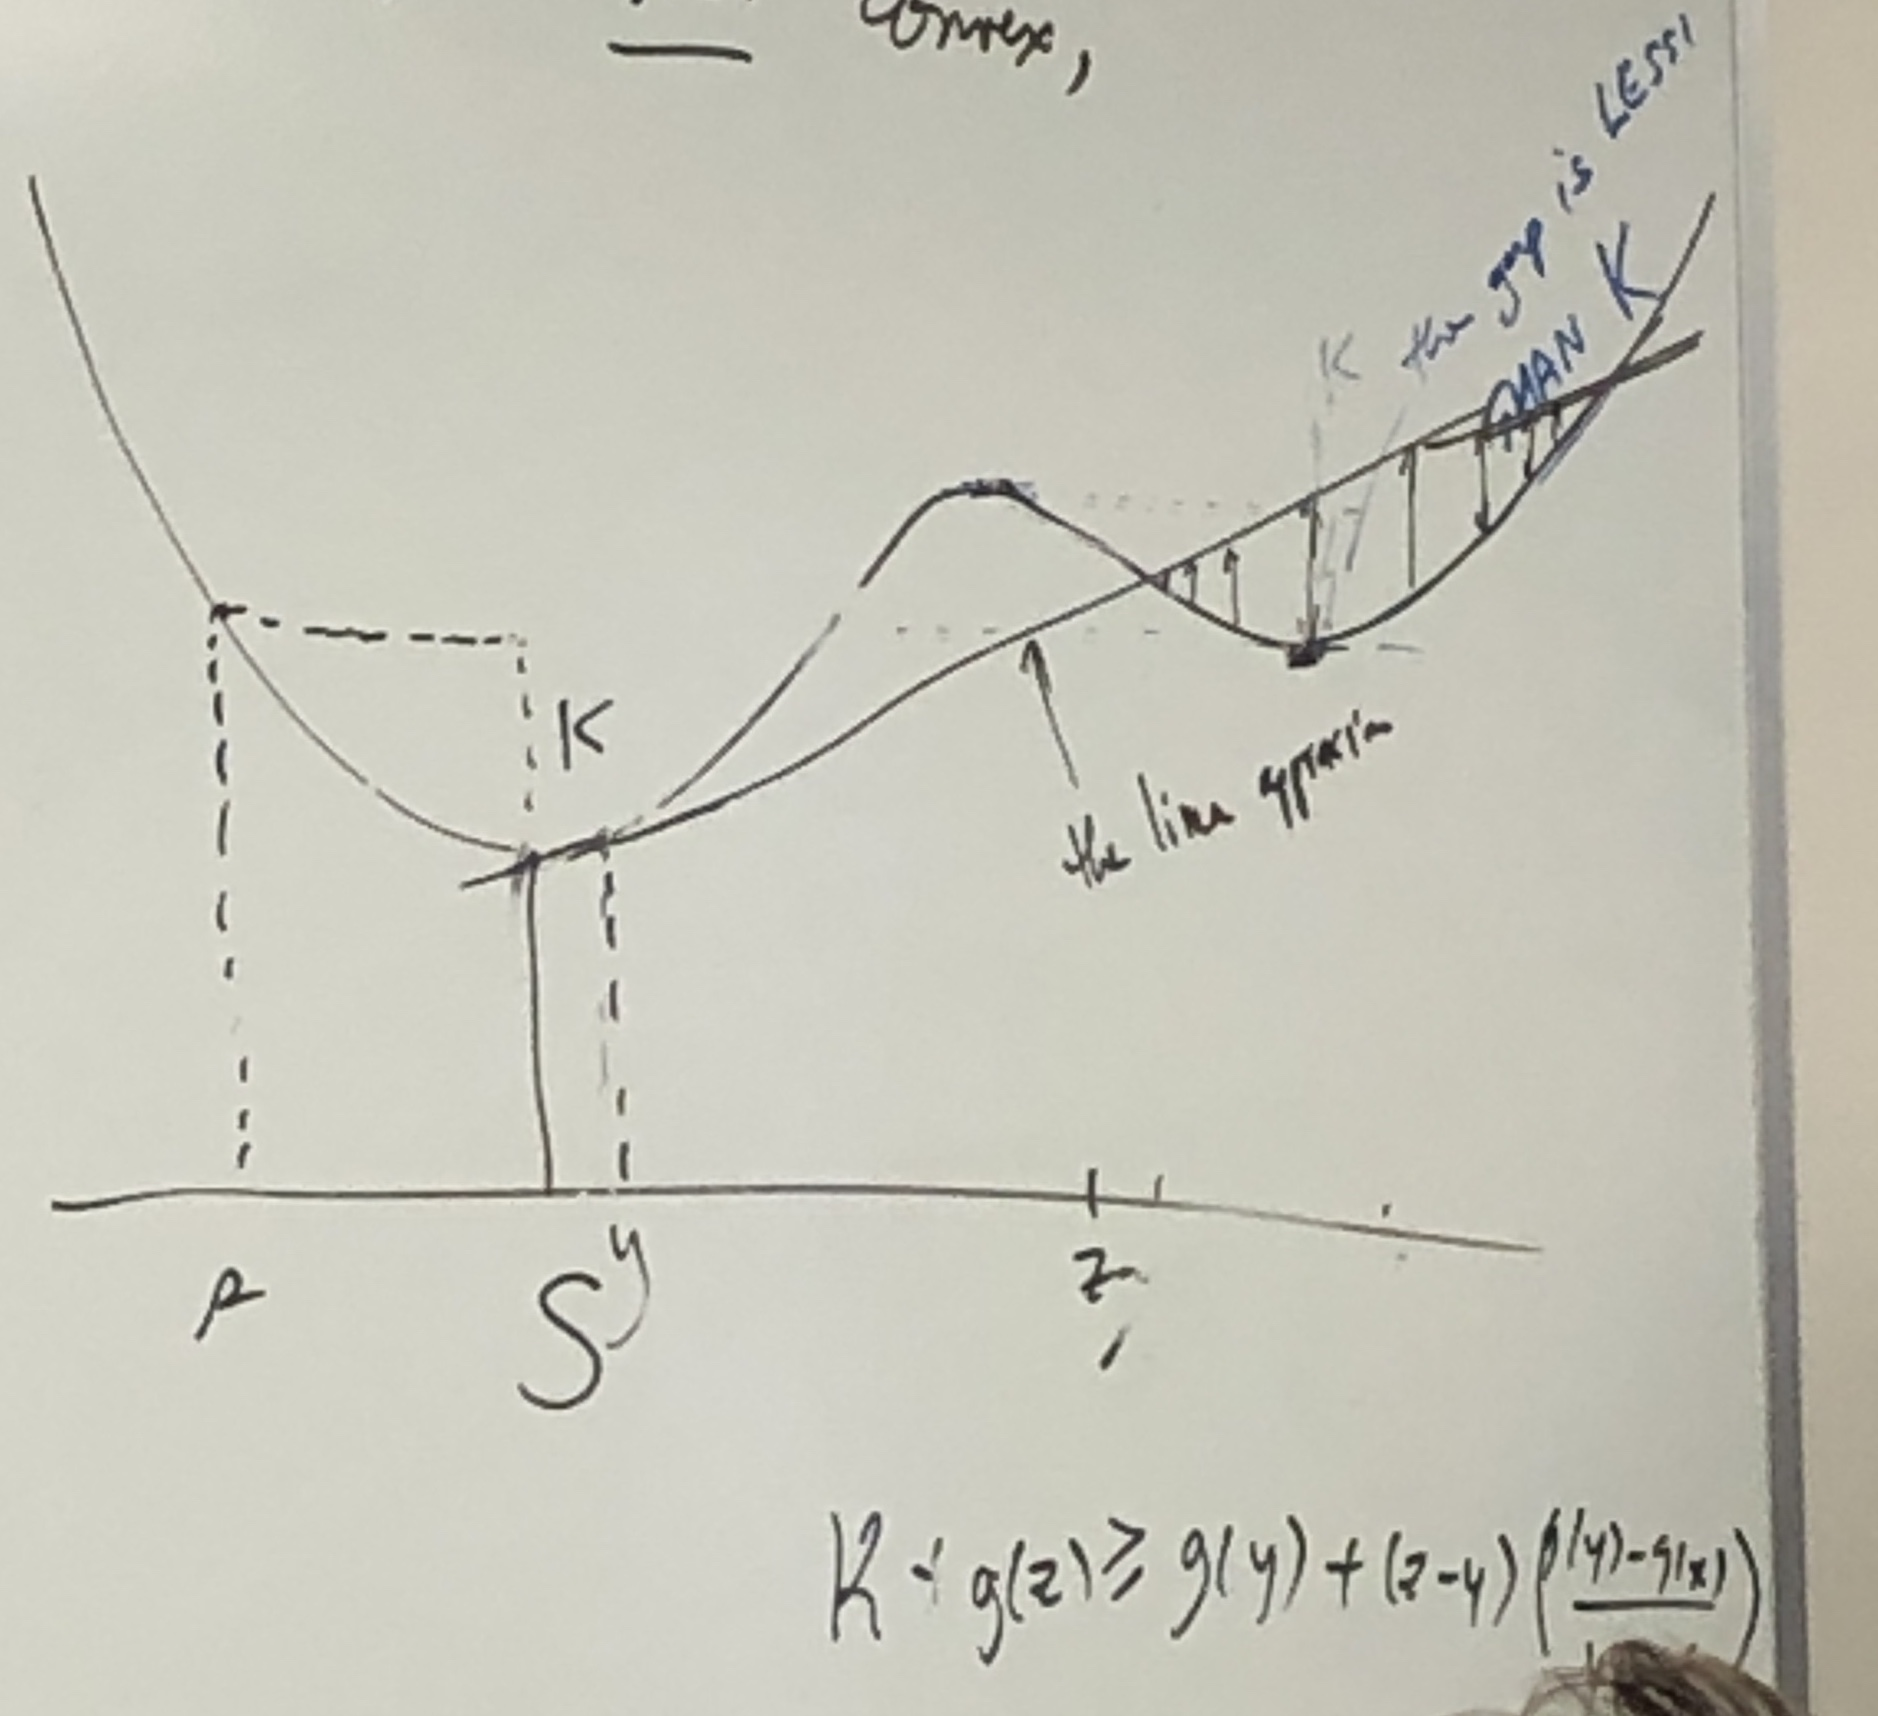
\includegraphics[scale=0.2]{stoch_dp_k_cvx}
\caption{Function is \(K\)-convex (see Definition \ref{stoch.dp.k.cvx}), but not convex.}
\label{stoch_dp_k_cvx_fig}
\end{center}
\end{figure}



See Figure \ref{stoch_dp_k_cvx_fig} for an example of a function that is \(K\)-convex but not convex.

\end{definition}

Intuitively, from (\ref{stoch.dp.k.cvx.2}) we can think of this as meaning that the linear approximation of \(g\) at \(z' = z + y\) by a secant line between \(y\) and \(x = y - b\) is no more than \(K\) greater than \(g(z+y)\). To make further sense of this definition, observe from (\ref{dp.k.cvx.defn}) that if \(K = 0\)

\begin{align*}
&  g(z+y) \geq g(y) + z \left( \frac{ g(y) - g(y-b)}{b} \right)
\\ \iff \qquad &  \frac{  g(z+y) - g(y)}{z} \geq   \frac{ g(y) - g(y-b)}{b} ;
\end{align*}

that is, the slopes of the secant lines are nondecreasing, which we know from Lemma \ref{cvx.slope.nondec} is true of convex functions. For the general case we have

\[
 \frac{ K + g(z+y) - g(y)}{z} \geq   \frac{ g(y) - g(y-b)}{b} .
 \]

Next we will show some results about \(K\)-convex functions that will be useful.
%Consider a function as shown in Figure \ref{dp_k_convexity_fig}.

\begin{proposition}[\textbf{Lemma 3.2.1 in \citet{v1_bertsekas2012dynamic}}]\label{stoch.dp.prop.k.cvx}

Properties of \(K\)-convex functions:

\begin{enumerate}[(a)]

\item A convex function \(g\) is 0-convex and \(K\)-convex for all \( K \geq 0\).

\item If \(g_1\) is \(K\)-convex and \(g_2\) is \(L\)-convex, then \(\alpha g_1 + \beta g_2\) is \((\alpha K + \beta L )\)-convex for all \(\alpha > 0\), \(\beta >0\).

\item If \(g\) is \(K\)-convex and \(w\) is a random variable, then \(y \mapsto \E_w[ g(y- w)]\) is also \(K\)-convex if \(\E_w |g(y-w)| < \infty\) for all \(y\). (Proof: exercise)

\item If \(g\) is a continuous \(K\)-convex function with \(g(y) \to \infty\) as \(|y| \to \infty\), then there exist scalars \((s, S)\) with \(s \leq S\) such that 

\begin{enumerate}[(1)]

\item \(g(S) \leq g(y)\) for all \(y\),

\item \(g(S) + K = g(s) \leq g(y)\) for all \(y < s\). (See Figure \ref{stoch_dp_k_cvx_p3_fig}.)

\item \(g(y)\) is decreasing on \((- \infty, s)\). 



\item \(g(y) \leq g(z) + K\) for all \(y, z\) with \(s \leq y \leq z\).

\end{enumerate}



\end{enumerate}

\begin{figure}[htbp]
\begin{center}
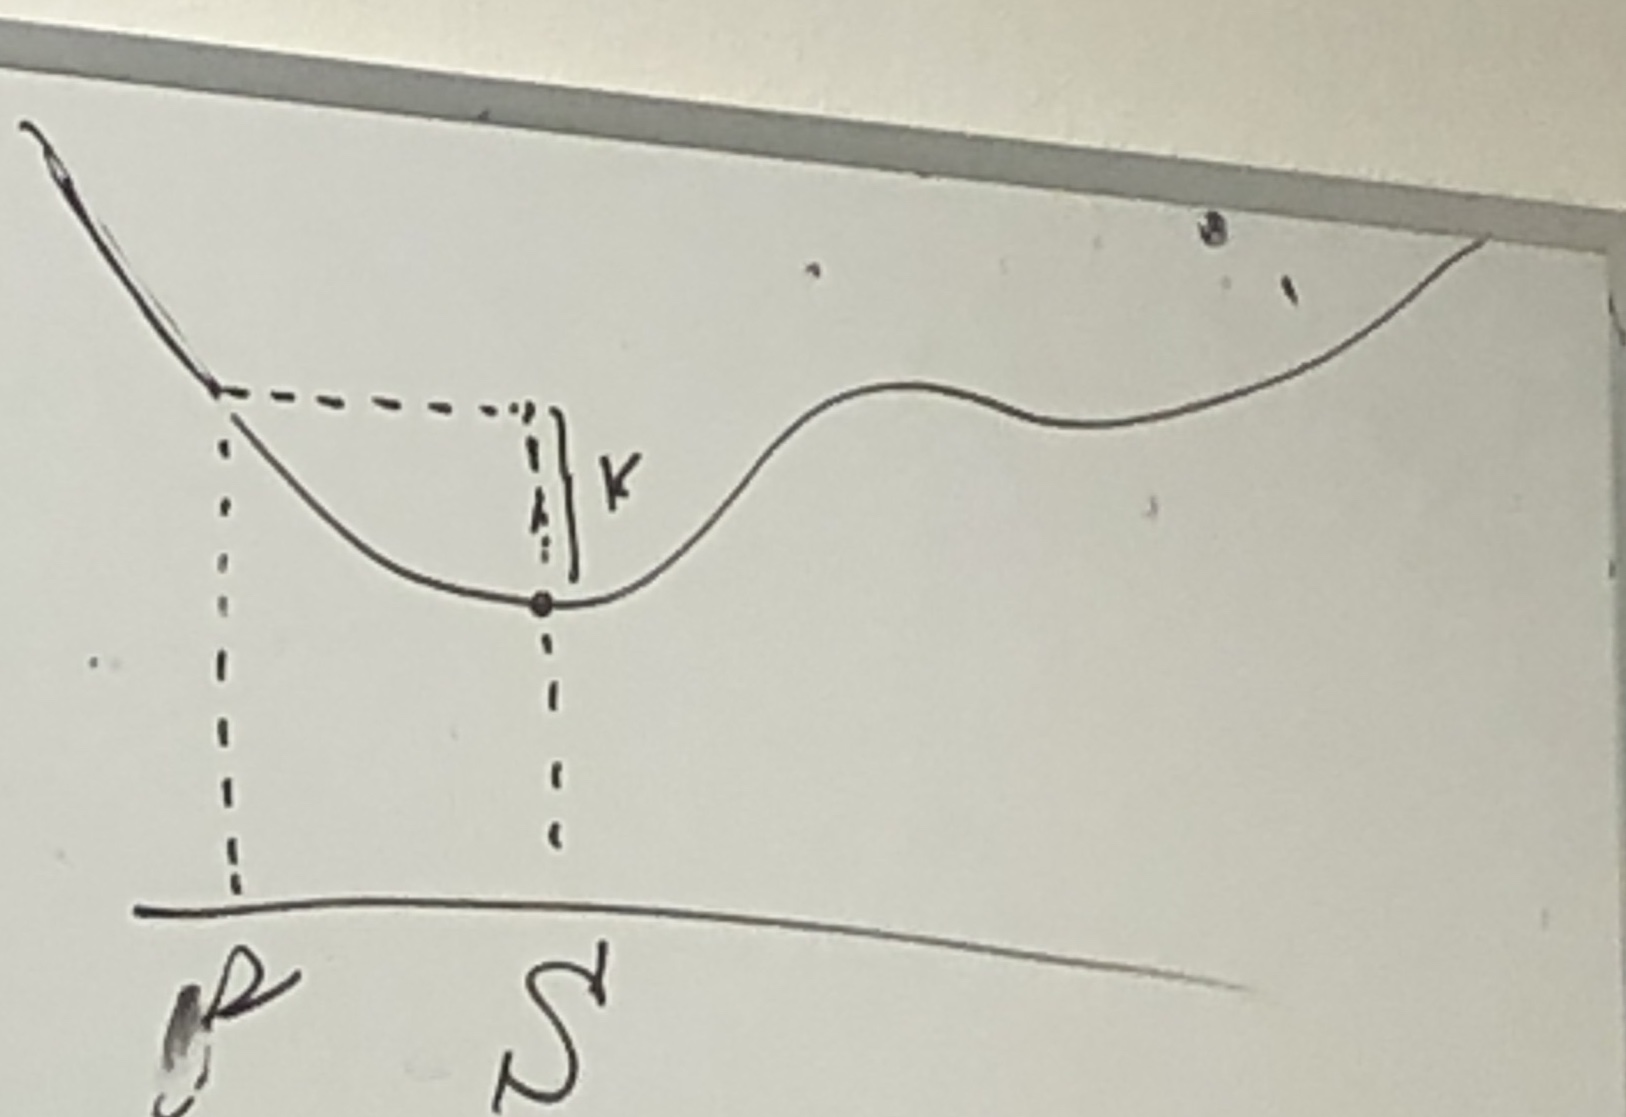
\includegraphics[scale=0.2]{stoch_dp_k_cvx_p3}
\caption{default}
\label{stoch_dp_k_cvx_p3_fig}
\end{center}
\end{figure}

\end{proposition}

\begin{proof}[Proof of part (d)]



\begin{enumerate}[(1)]

\item Since \(g\) is continuous and \(\lim_{|y| \to \infty} g(y) = \infty\), there exists a minimizing point \(S\) of \(g\) with minimum \(g(S)\). 

\item Define \(s := \min\{ z: g(z) = g(S) + K\}\). Note that \(s \leq S\). For all \(y < s \leq S\), by \(K\)-convexity of \(g\) and the definition of \(s\), from (\ref{stoch.dp.k.cvx.2}) we have 

\begin{align*}
K + g(S) & \geq g(s) + (S - s) \left(  \frac{g(s) - g(y)}{s - y} \right) \\
\iff 0 & \geq \underbrace{\frac{S-s}{s-y}}_{\geq 0 } \cdot [g(s) - g(y)] \\
\iff g(y) & \geq g(s).
\end{align*}

\item For any \(y_1, y_2\) satisfying \(y_1 < y_2 < s \leq S\), by \(K\)-convexity from (\ref{stoch.dp.k.cvx.2}) we have

\[
K + g(S) \geq g(y_2) + \frac{S - y_2}{y_2 - y_1} (g(y_2) - g(y_1)).
\]

By (2) above, \(g(y_2) > g(s) = g(S) + K\). Therefore

\[
0 > g(S) + K - g(y_2) \geq \underbrace{ \frac{S - y_2}{y_2 - y_1}}_{> 0} (g(y_2) - g(y_1)), \qquad \implies g(y_1) > g(y_2).
\]

\item Note that \(g(y) \leq g(z) + K\) holds when \(y = z\) (trivially), \(y= S\) (because \(S\) is a global minimizer of \(g\)), or \(y = s\) (because \(g(S) + K = g(s) \leq g(z) + K\) for all \(z\)). Since \(s \leq y \leq z\), we only need to consider two cases.

\begin{itemize}

\item \textbf{Case 1:} Assume \(S < y < z\). By \(K\)-convexity from (\ref{stoch.dp.k.cvx.2}), 

\begin{align*}
K + g(z) & \geq g(y) + \underbrace{(z-y)}_{> 0 \text{ (assumption)}} \cdot \left(\frac{ \overbrace{g(y) - g(S)}^{> 0 \text{ (} S \text{ global min)}}}{\underbrace{y - S}_{> 0 \text{ (assumption)}}} \right) \\
& \geq g(y).
\end{align*}

\item \textbf{Case 2:} Assume \(s < y < S\). By \(K\)-convexity from (\ref{stoch.dp.k.cvx.2}),

\begin{align*}
& g(s) = K + g(S) \geq g(y) + (S- y) \left( \frac{g(y) - g(s)}{y - s} \right) \\
\iff \qquad &  \left( 1 - \frac{\overbrace{y -S}^{>0} }{\underbrace{y-s}_{> y - S}} \right) g(s) \geq   \left( 1 - \frac{y -S }{y-s} \right) g(y) 
\\ \iff  \qquad & g(s) \geq g(y)  .
\end{align*}

Then \(g(y) \leq g(s) = g(S) + K \leq g(z) + K\).

\end{itemize}

\end{enumerate}

\end{proof}


We are now ready to analyze inventory control with fixed costs. Suppose that 

\[
C(u) = \begin{cases}
K + cu, & u > 0, \\
0, & \text{otherwise}
\end{cases}
\]

so \(k\) is the fixed cost. 

\begin{theorem}\label{stoch.dp.them.opt.fix.cost}



When there is a fixed cost of order, an \((s, S)\) policy is optimal; that is, for any period \(k\) there exists a pair of thresholds \((s_k, S_k)\) with \(s_k \leq S_k\) such that 

\begin{equation}\label{dp.fixed.costs.inv.opt.policy}
\mu_k^*(x_k) = \begin{cases}
S_k - x_k, & x_k \leq s_k, \\
0, & \text{otherwise.}
\end{cases}
\end{equation}

\end{theorem}

\begin{proof}

Again let \(y := x_k + u_k\). Define \(G_k: \mathbb{R} \to \mathbb{R}\) as follows;

\begin{equation}\label{dp.def.g_k.fixed.costs}
G_k(y) := cy + \underset{w_k}{\E}[ \mathcal{G}(y - w_k) + J_{k+1}(y - w_k)].
\end{equation}

Then 

\begin{align*}
J_N(x_N) & = 0, \\
J_k(x_k) & = \min_{u_k > 0} \left\{ C(u_k) + \E\left[ \mathcal{G}(x_k + u_k) \right] + \E\left[J_{k+1}(x_k + u_k - w_k) \right] \right\} \\
%& \vdots \\
& = \min \left\{ G_k(x_k) - c x_k, \min_{u_k > 0} \left\{ K + G_k(x + u_k) - c x_k \right\}\right\}
\\ & = - c x_k + \min \left\{G_k(x_k), \min_{y > x_k} [k + G_k(y)] \right\}, \qquad k \in \{0, \ldots, N=1\}.
\end{align*}

where the third line follows because the cost is the minimum of the cost if no order is made (the cost on the left) or the cost if an order is made (the cost on the right), and the fourth line follows by the change of variable \(y := x_k + u_k\).

\begin{figure}[htbp]
\begin{center}
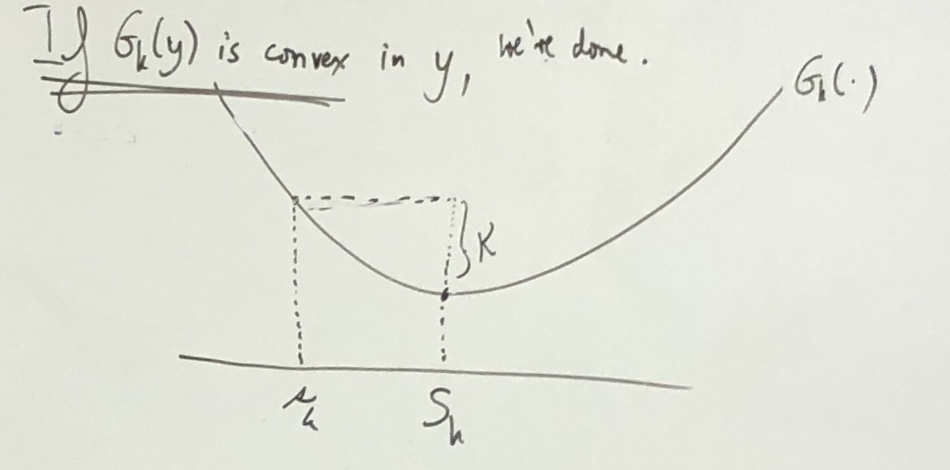
\includegraphics[scale=0.3]{stoch_dp_fixed}
\caption{If \(G_k(\cdot)\) is convex, the policy (\ref{dp.fixed.costs.inv.opt.policy}) is optimal, where \(S_k\) is a minimizer of \(G_k(\cdot)\) and \(s_k\) is the smallest value of \(y\) for which \(G_k(y) = K + G_k(S_k)\). However, \(G_k\) is not necessarily convex.}
\label{dp_k_convexity_fig}
\label{stoch_dp_fixed_fig}
\end{center}
\end{figure}




If \(G_k(y)\) is convex in \(y\), the result follows quickly, as in the no fixed costs case covered in Theorem \ref{stoch.dp.order.up.to.opt} (see Figure \ref{stoch_dp_fixed_fig}). In particular, the policy (\ref{dp.fixed.costs.inv.opt.policy}) is optimal, where \(S_k\) is a minimizer of \(G_k(\cdot)\) and \(s_k\) is the smallest value of \(y\) for which \(G_k(y) = K + G_k(S_k)\). 



%(see Figure \ref{dp_k_convexity_fig}).
%
%\begin{figure}[htbp]
%\begin{center}
%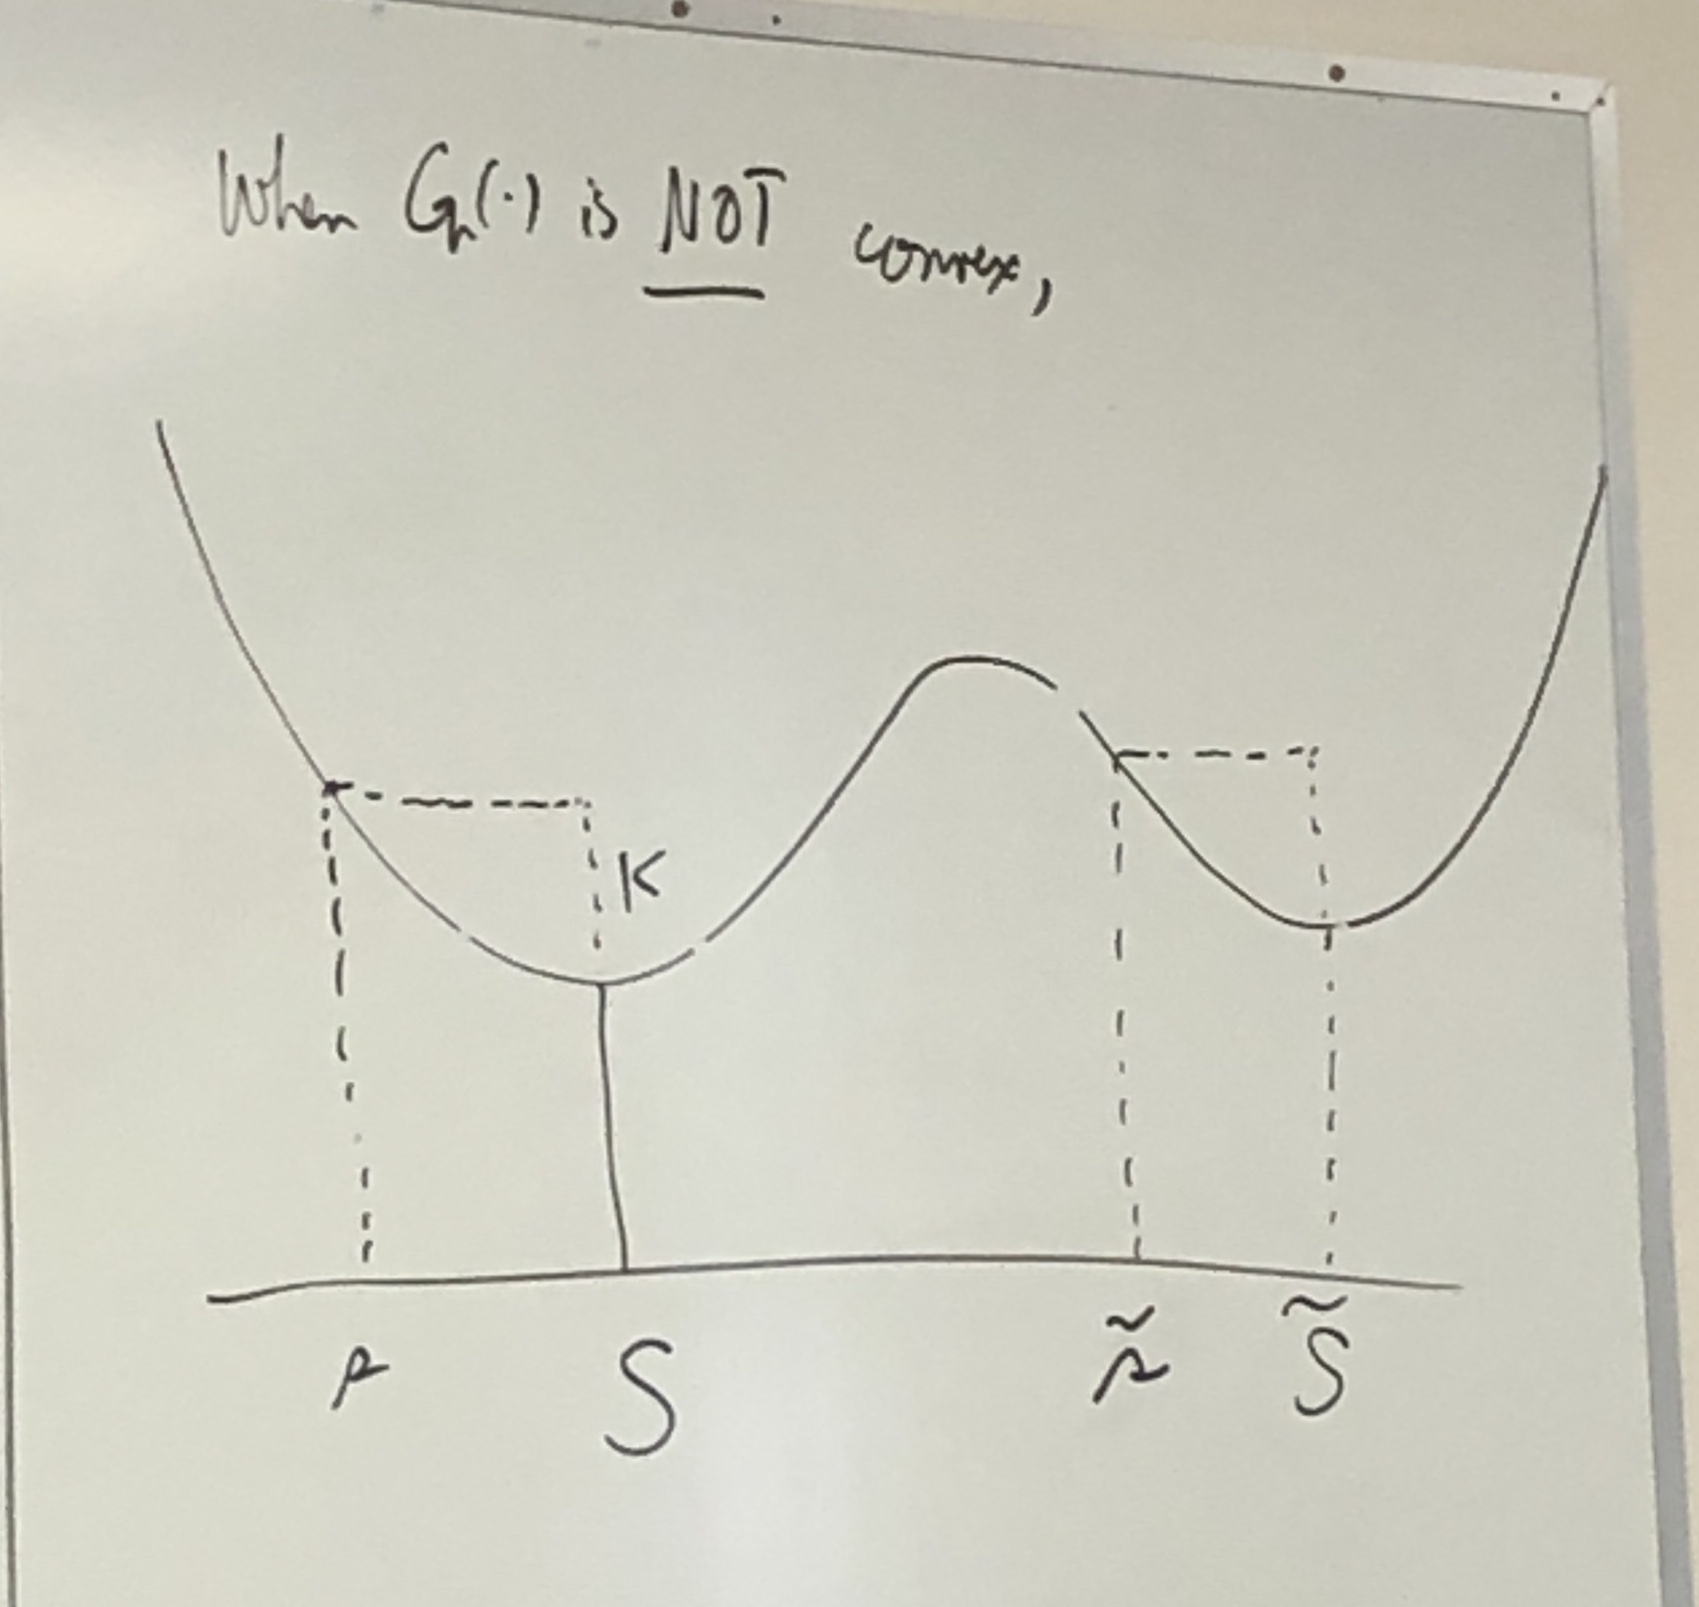
\includegraphics[scale=0.2]{stoch_dp_fixed_ncvx}
%\caption{default}
%\end{center}
%\end{figure}

\begin{figure}[htbp]
\begin{center}
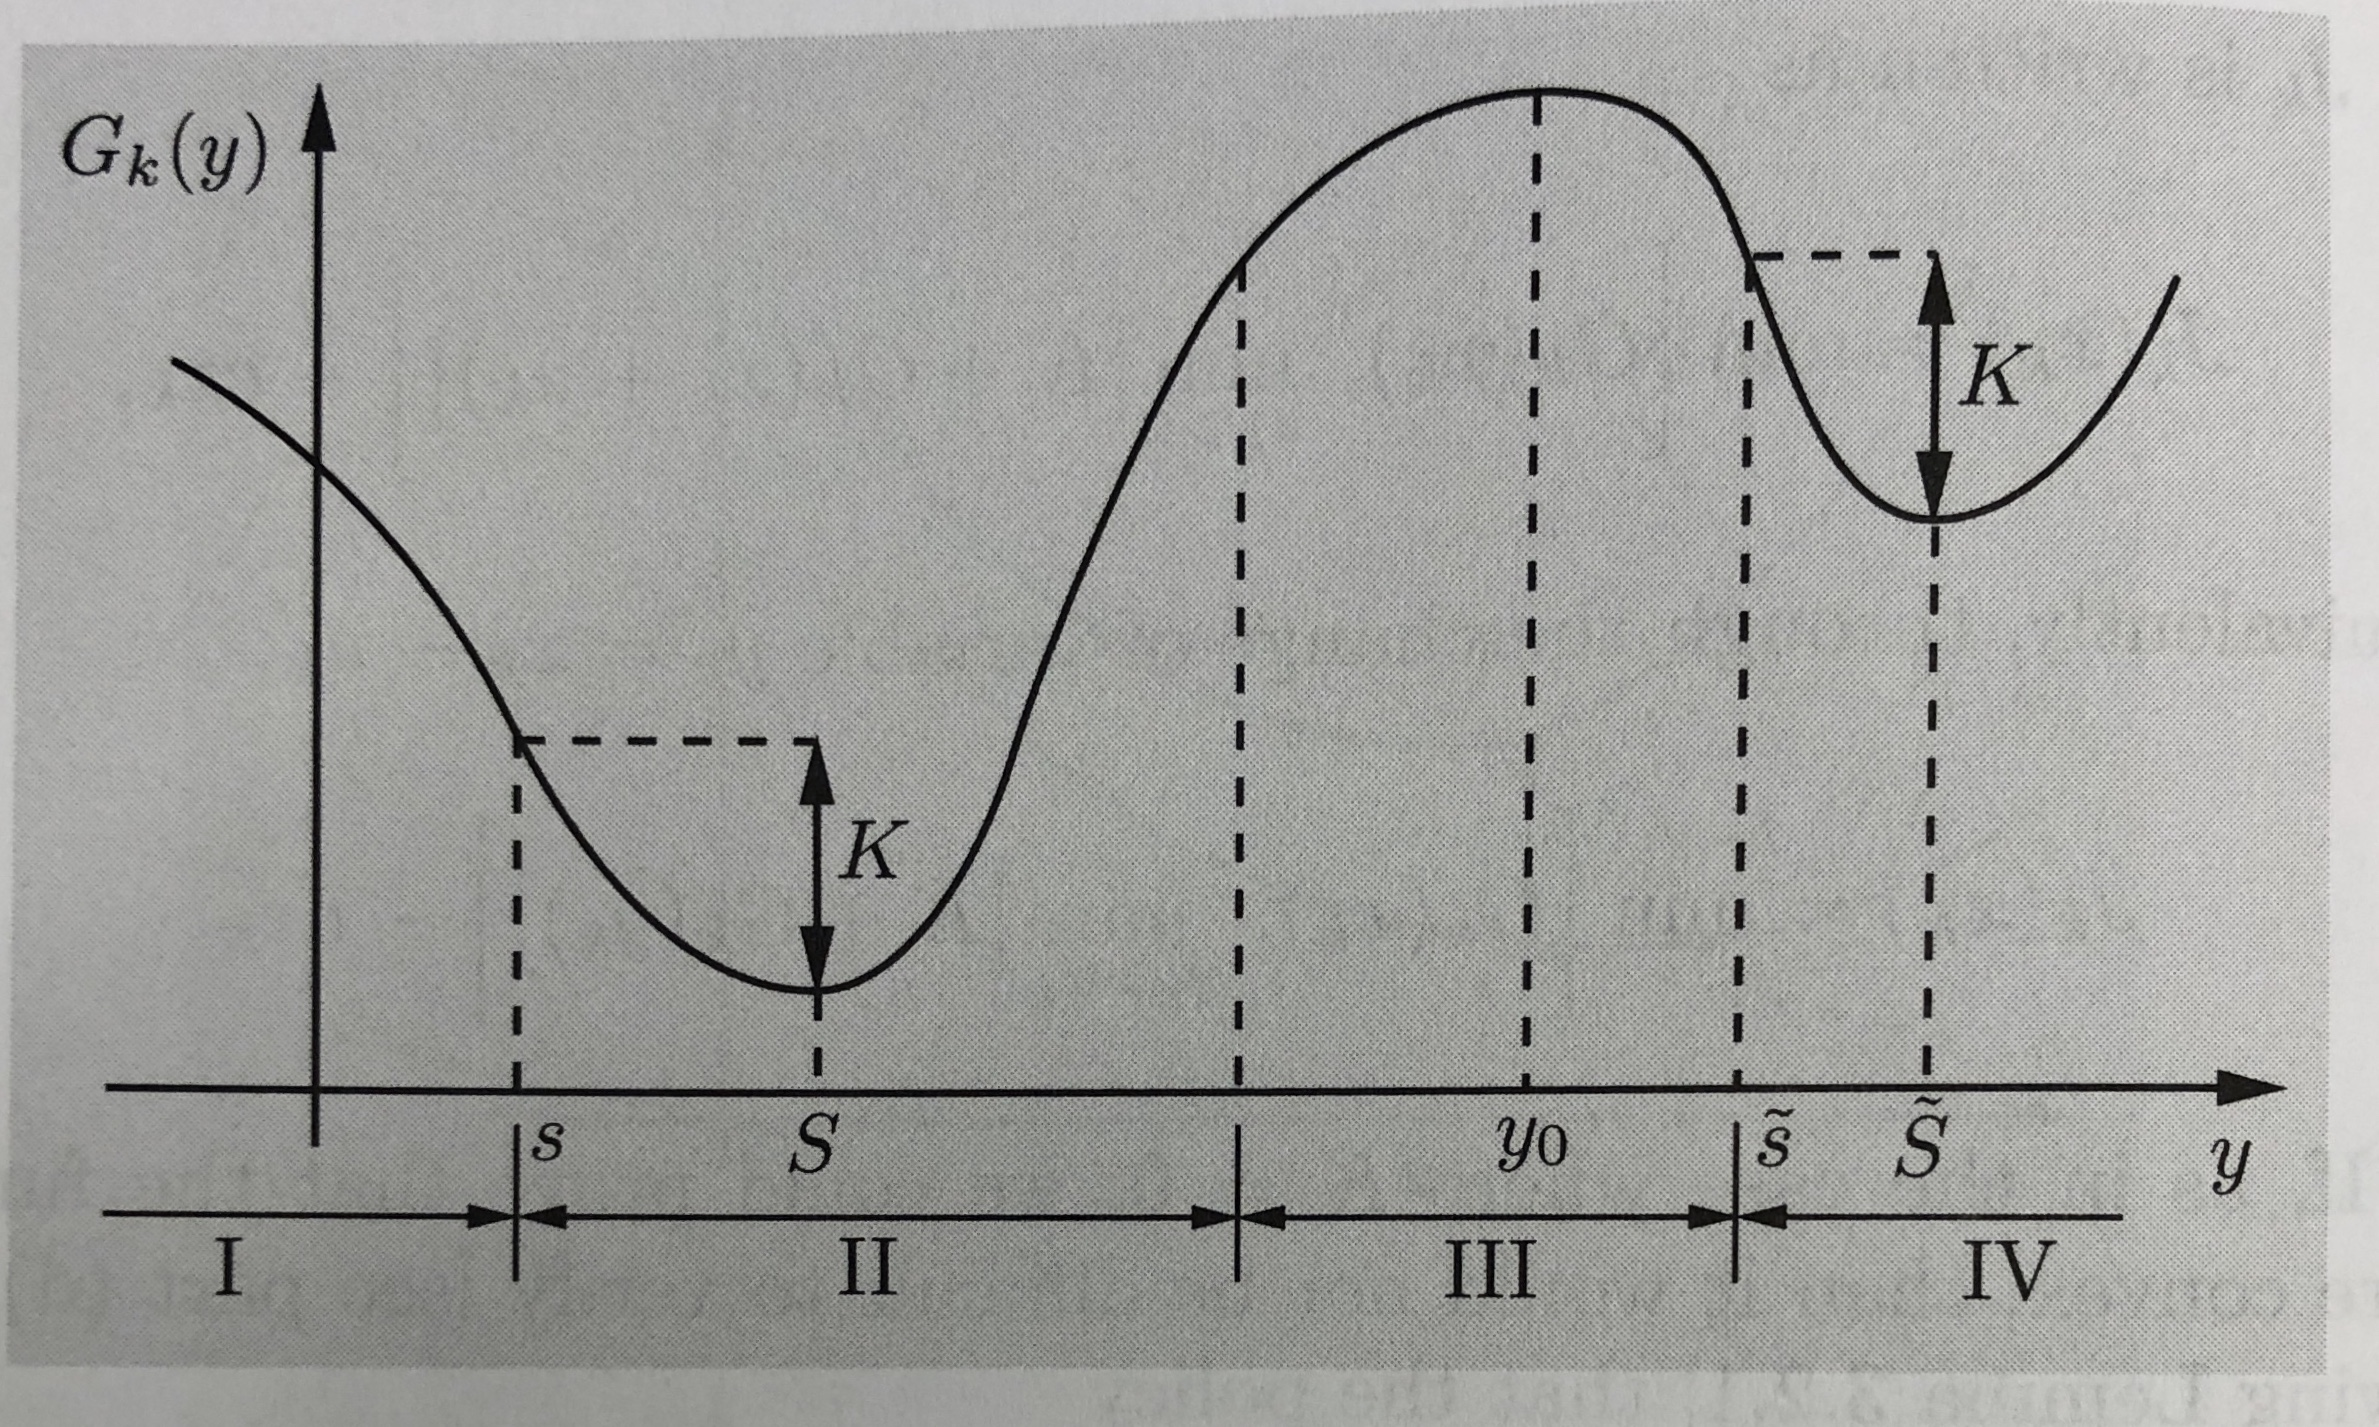
\includegraphics[scale=0.17]{dp_k_convexity}
\caption{Figure 3.2.2 in \citet{v1_bertsekas2012dynamic}.}
\label{dp_k_convexity_fig}
\end{center}
\end{figure}

However, when \(K > 0\) it is not necessarily true that \(G_k\) is convex. This means it could have multiple minima. Consider Figure \ref{dp_k_convexity_fig}. If it were true that \(G_k\) had a form like this, the optimal policy would be to order \((S-x)\) in interval I, zero in intervals II and IV, and \((\tilde{S}-x)\) in interval III.

But it turns out \(G_k(\cdot)\) is \(K\)-convex, so the form of \(G_k\) in Figure \ref{dp_k_convexity_fig} is impossible. If \(y_0\) is the local maximum in in the interval III, we must have for sufficiently small \(b > 0\)

\[
\frac{G_k(y_0) - G_k(y_0 - b)}{b} \geq 0,
\]

and from the definition of \(K\)-convexity (\ref{dp.k.cvx.defn}) it follows that 

\[
K + G_k(\tilde{S}) \geq G_k(y_0),
\] 

contradicting the construction shown in Figure \ref{dp_k_convexity_fig}. Then the result will follow from (d)(4) of Proposition \ref{stoch.dp.prop.k.cvx}, because it is optimal to order up to the minimum if you have less inventory than \(s_k\), but just to the right of \(s_k\) the cost of ordering exceeds the savings from ordering, and part (d)(4) of Proposition \ref{stoch.dp.prop.k.cvx} guarantees that the cost of ordering will never again go below the savings from ordering. So the result is immediate from Lemma \ref{dp.lemma.k.cvx.inventory}.











% Fortunately, \(G_k(y)\) satisfies \(K\)-convexity.

\end{proof}

\begin{lemma}\label{dp.lemma.k.cvx.inventory}

\(G_k\) are continuous and \(K\)-convex for all \(k\), and \(G_k(y) \to \infty\) as \(|y| \to \infty\). Further, \(J_k(\cdot)\) are continuous and \(K\)-convex for all \(k\). 

\end{lemma}








 
 
 
 \begin{proof}[Proof of Lemma \ref{dp.lemma.k.cvx.inventory}]

 We will prove the result by induction. The base case is trivial since \(J_N(\cdot) = 0\). Suppose \(J_{\ell+1}(\cdot)\) is \(K\)-convex. Then

\[
G_\ell(y) = \underbrace{cy}_{0-\text{convex}} +  \underbrace{\underset{w_\ell}{\E} \mathcal{G}(y - w_l) }_{0-\text{convex}} + \underbrace{\underset{w_\ell}{\E} \left[ J_{\ell+1}(y - w_\ell) \right]}_{K\text{-convex by (c) of Proposition \ref{stoch.dp.prop.k.cvx}}}
\]

Therefore \(G_\ell(y)\) is \(K\)-convex. Therefore by (d) of Proposition \ref{stoch.dp.prop.k.cvx}, there exist \((s_\ell, S_\ell)\) such that 

\[
G_\ell(S_\ell) = \min_y G_\ell(y) , \qquad G_\ell(s_\ell) = G_\ell(S_\ell) + K.
\]

Then

\begin{align}
J_\ell(x_\ell) & = -c \cdot x_\ell + \min\{ G_\ell (x_\ell), \min_{y > x_\ell} [K + G_\ell(y) ] \} \nonumber \\
& = -c x_\ell + \begin{cases}
\underbrace{K + G_\ell(S_\ell)}_{=G_\ell(s_\ell)}, & x_\ell \leq s_\ell, \\
G_\ell(x_\ell), &  x_\ell > s_\ell
\end{cases} \nonumber 
\\
& = -c x_\ell + \begin{cases}
G_\ell(s_\ell), & x_\ell \leq s_\ell, \\
G_\ell(x_\ell), &  x_\ell > s_\ell. \label{stoch.dp.fixed.thm.proof.1}
\end{cases}
\end{align}



\begin{figure}[htbp]
\begin{center}
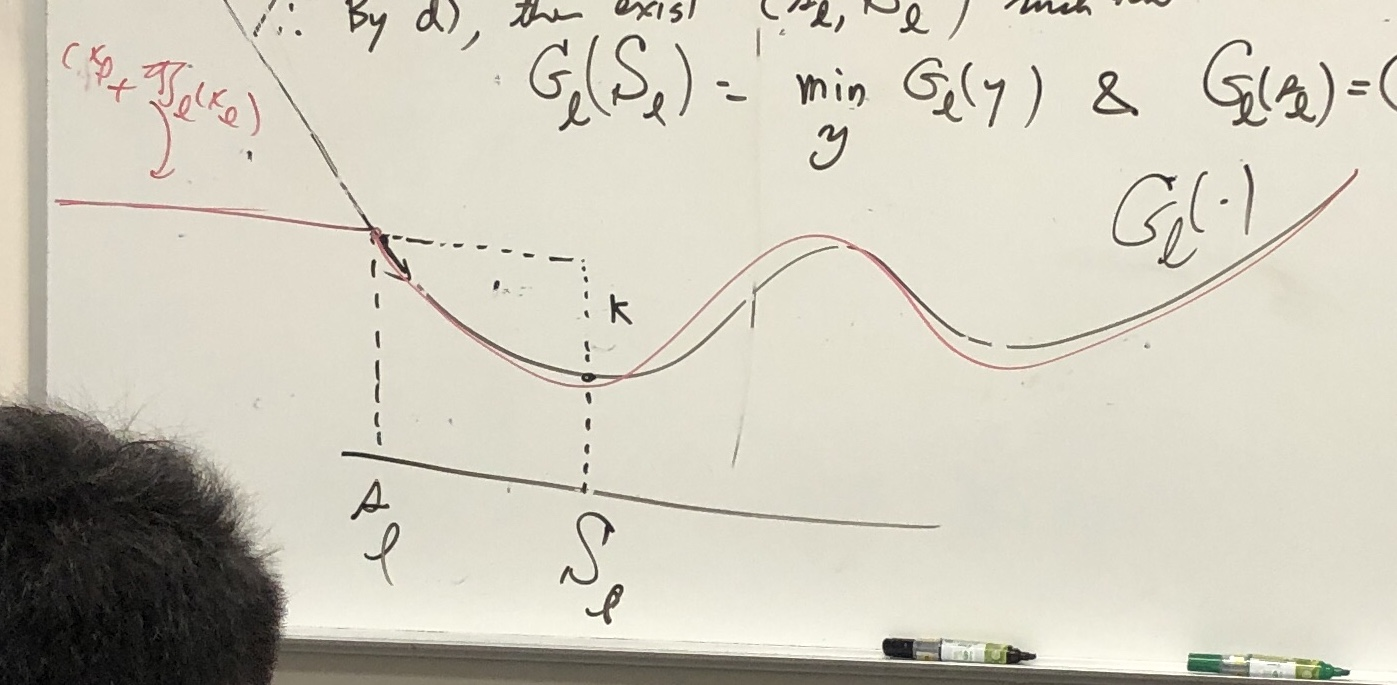
\includegraphics[scale=0.2]{stoch_dp_fixed_thm_proof_1}
\caption{The red line is the right part of (\ref{stoch.dp.fixed.thm.proof.1}) (\(J_\ell(x_\ell) + c x_\ell\)).}
\label{stoch_dp_fixed_thm_proof_1}
\end{center}
\end{figure}

(See Figure \ref{stoch_dp_fixed_thm_proof_1} for an illustration of \(J_\ell\).) \(J_{\ell}\) is continuous. Is \(J_\ell(\cdot)\) convex? No. Consider the point \(s_\ell\). Left derivative of \(J_\ell\) at \(s_\ell\) is \(-c + 0\), right derivative is \(-c + \lim_{x \to s_\ell^+} G_\ell'(x) < -c + 0\) (because \(G_\ell\) is still decreasing at \(s_\ell\)---again see Figure \ref{dp_k_convexity_fig}). If the function were convex, the derivative would be nondecreasing, so this violates convexity. 




However, we can show that \(J_{\ell}\) is \(K\)-convex. We know from Equation (\ref{dp.k.cvx.defn}) in Definition \ref{stoch.dp.k.cvx} that we must verify



\begin{equation}\label{stoch.dp.fixed.thm.proof.2}
K + J_\ell(y+z) \geq J_\ell(y) + z \left( \frac{J_\ell(y) - J_\ell(y- b)}{b} \right)
\end{equation}

for all \(y \in \mathbb{R}\), for all \(z \geq 0, b \geq 0\). There are three cases to consider.

\begin{enumerate}

\item \(y \geq s_\ell\): Then \(y + z \geq s_\ell\). If \(y - b \geq s_\ell\), then examining (\ref{stoch.dp.fixed.thm.proof.1}), the function \(J_\ell(\cdot)\) at these points is \(-c x_\ell + G_\ell(x_\ell)\) (the sum of a linear function and a \(K\)-convex function), so (\ref{stoch.dp.fixed.thm.proof.2}) holds and \(K\)-convexity follows. Suppose \(y - b < s_\ell\). We need to verify (\ref{stoch.dp.fixed.thm.proof.2}); that is,

\begin{align}
K + J_\ell(y+z)  & \geq J_\ell(y) + z \left( \frac{J_\ell(y) - J_\ell(y- b)}{b} \right) \nonumber \\
\iff \text{(by (\ref{stoch.dp.fixed.thm.proof.1}))} \qquad K + \underbrace{G_\ell(y+z) - c(y +z)}_{= J_\ell(y +z), \text{ since } y + z \geq s_\ell} & \geq \underbrace{G_\ell(y)  - cy}_{= J_\ell(y ), \text{ since } y  \geq s_\ell}  + z \left( \frac{\overbrace{G_\ell(y) - cy}^{= J_\ell(y ), \text{ since } y  \geq s_\ell} - \overbrace{G_\ell(s_\ell) + c(y-b)}^{= J_\ell(y - b ), \text{ since } y - b  < s_\ell}}{b} \right) \nonumber \\
 \iff \qquad K + G_\ell(y+z) - cz & \geq G_\ell(y) +  z \left( \frac{G_\ell(y) - G_\ell(s_\ell)}{b} - c \right) \nonumber \\
\iff \qquad K + G_\ell(y+z) & \geq G_\ell(y) +  z \left( \frac{G_\ell(y) - G_\ell(s_\ell)}{b} \right), \label{stoch.dp.fixed.thm.proof.3}
\end{align}

so proving (\ref{stoch.dp.fixed.thm.proof.3}) is equivalent to proving \(K\)-convexity. We will look at two sub-cases:

\begin{itemize}

\item \textbf{Sub-case 1:} \(G_\ell(y) \geq G_\ell(s_\ell) \). By \(K\)-convexity of \(G_\ell\), using (\ref{stoch.dp.k.cvx.2}), 

%\[
%K + G_\ell(y+z) \geq G_\ell(y) +  z \left( \frac{G_\ell(y) - G_\ell(y- b)}{b} \right) 
%\]
%
%\[
%K +  \geq g(y) + (z'-y) \left(  \frac{g(y) - g(x)}{y - x} \right)
%\]

\[
K +  G_\ell(y+z) \geq  G_\ell(y)  + z \left(  \frac{G_\ell(y) - G_\ell(s_\ell) }{y - s_\ell} \right) \geq  G_\ell(y)  + z \left(  \frac{G_\ell(y) - G_\ell(s_\ell) }{b} \right)
\]

%\[
%K + G_\ell(y+z) \geq G_\ell(y) +  z \left( \frac{G_\ell(y) - G_\ell(y- b)}{b} \right) \geq G_\ell(y) +  z \left( \frac{G_\ell(y) - G_\ell(s_\ell)}{b} \right),
%\]

where the last step follows because \(y - b < s_\ell \iff 1/(y - s_\ell) >  1/b\).

\item  \textbf{Sub-case 2:} \(G_\ell(y) < G_\ell(s_\ell)\). Then

\begin{align*}
K + G_\ell(y + z) & \geq K + G_\ell(S_\ell)
\\ & =   G_\ell(s_\ell)
\\ & > G_\ell(y) & \text{(by assumption of sub-case)}
\\ & \geq G_\ell(y) + z \left(\frac{\overbrace{ G_\ell(y) - G_\ell(s_\ell)}^{< 0}}{b} \right),
\end{align*}

verifying (\ref{stoch.dp.fixed.thm.proof.3}) and proving \(K\)-convexity in this case.

\end{itemize}

\item \(y \leq y+z \leq s_\ell\): In this region, from (\ref{stoch.dp.fixed.thm.proof.1}) we see that \(J_\ell\) is linear because \(y - b \leq y \leq y + z \leq s_\ell\), so all of the \(J_\ell\) in (\ref{stoch.dp.fixed.thm.proof.2}) are in the region where \(J_\ell\) is constant, so \(K\)-convexity should hold trivially. Let's check: (\ref{stoch.dp.fixed.thm.proof.2}) becomes

\begin{multline*}
K -c(y+z) + G_\ell(s_\ell) \geq -cy +  G_\ell(s_\ell)+ z \left( \frac{-cy +  G_\ell(s_\ell)  + c(y - b) -  G_\ell(s_\ell)}{b} \right)
\\ \iff \qquad K -cz \geq     z \left( \frac{   -cb }{b} \right),
\end{multline*}

so the inequality holds as desired, proving \(K\)-convexity in this case.

\item \(y \leq s_\ell \leq y + z\): To establish \(K\)-convexity, from (\ref{stoch.dp.fixed.thm.proof.2}) we need to have

\begin{align}
K + J_\ell(y+z) & \geq J_\ell(y) + \frac{z}{b} \left( J_\ell(y) - J_\ell(y-b)\right) \nonumber \\
\iff K+ \underbrace{G_\ell(y+z) - c(y+ z)}_{=J_\ell(y+z) \text{ since } y + z \geq s_\ell }  & \geq \underbrace{G_\ell(s_\ell) - cy}_{=J_\ell(y) \text{ since } y  \leq s_\ell }  + \frac{z}{b} \left( \underbrace{G_\ell(s_\ell) - cy}_{=J_\ell(y) \text{ since } y  \leq s_\ell }  - \underbrace{G_\ell(s_\ell) + c(y-b)}_{=J_\ell(y-b) \text{ since } y -b \leq s_\ell } \right) \nonumber \\
\iff K+ G_\ell(y+z) - c(y+ z) & \geq G_\ell(s_\ell) - cy -c z \nonumber \\
\iff K+ G_\ell(y+z) & \geq G_\ell(s_\ell) \label{stoch.dp.fixed.thm.proof.4}
\end{align} 

But (\ref{stoch.dp.fixed.thm.proof.4}) is always true because \(G_\ell(s_\ell) = G_\ell(S_\ell) + K \leq G_\ell(y+z) + K\) (since \(G_\ell(S_\ell)\) is a global minimum), proving \(K\)-convexity in this case.

\end{enumerate}

Therefore we have established \(K\)-convexity (and continuity) of both \(G_\ell(\cdot)\) and \(J_\ell(\cdot)\). It also holds that \(G_\ell(y) \to \infty \) as \(|y| \to \infty\). Now recall (\ref{dp.def.g_k.fixed.costs}): this shows that \(G_{\ell-1}(\cdot)\) is \(K\)-convex, since it is the sum of something linear, something \(K\)-convex (by Proposition \ref{stoch.dp.prop.k.cvx} (c)), and something \(K\)-convex (as we just showed). But since \(w_{\ell-1}\) is bounded, \(G_{\ell-1}\) is continuous and \(G_{\ell - 1}(y) \to \infty\) as \(|y| \to \infty\), so by the previous argument \(J_{\ell-1}\) is \(K\)-convex. We can repeat this continually to show the result.





\end{proof}

\begin{remark}

Also proved this in a 2000 paper ``A single-unit approach to multi..." but the proof technique does not generalize to other problems as well (the way this proof does).

\end{remark}

\subsection{Capacity Allocation and Revenue Management}

3 levels of revenue management:

\begin{enumerate}

\item Strategic: how to segment different markets and differentiate prices; which markets you go after, which subsets of customers, etc. (often done quarterly/annually.)

\item Tactical: (e.g. plane tickets: what's a good pricing strategy to maximize revenue? maybe save tickets for last minute when you can charge a lot?) calculate and update booking limits (done daily/weekly). Use forecasting, optimization, etc.

\item Booking Control/Execution: determine which booking to accept (done in real time)

\end{enumerate}

Today: focus on tactical. 3 components:

\begin{enumerate}

\item \textbf{Resources:} units of capacities managed by suppliers. Example: seats on a flight leg, hotel room nights, rental car days. (We're interested in setting when resources are constrained.)

\item \textbf{Products:} what customers purchase. Each product corresponds to a combination of resources, for example, a ticket from LAX to JFK, may involve a layover (so 2 legs/resources), etc.

\item \textbf{Fare classes:} there are fares associated with end product (not just price, also things like layover time, bringing a carry-on, etc.). Each fare class is a combination of a price and restrictions on what/who can purchase a product.

\end{enumerate}

A supplier controls

\begin{enumerate}

\item Sets of resources with a fixed and perishable capacity (e.g. plane seats perishable since can't sell tickets for seats on flights in the past).

\item A portfolio of products to offer to customers.

\item A set of fares associated with the end product. (has to do with setting prices, but main goal: the decision to open/close certain fare classes at each moment to maximize revenue.) Revenue: fare that you pay minus commission, etc.

\end{enumerate}

Three problems in tactical revenue management:

\begin{enumerate}

\item \textbf{Single resource capacity allocation:} how many customers from different fare classes should we allow to book? (``single resource" e.g. direct flight or single night stay in hotel.)

\item \textbf{Network revenue management:} how should bookings be managed across a network of resources? (no known exact solution yet. we'll discuss after midterms)

\item \textbf{Overbooking:} how to managed bookings when faced with uncertain future no-shows? (standard ad-hoc methods.)

\end{enumerate}

Today we'll focus on single resource capacity allocation.

\begin{example}[\textbf{Two-class capacity allocation (Littlewood's formula)}]\label{stoch.dp.two.class.littewood}

Suppose we have \(C\) seats on a plane flight leg on a given date. We have two fare classes: a discounted fair \(P_d\) and full fare \(P_f\), with \(P_f > P_d\). Suppose the discount fare demand is \(D_d\) (number of customers that will arrive with a discount fare) and the full fare demand is \(D_f\). Suppose \(D_d\) and \(D_f\) are independent, and suppose \(D_d\) customers arrive before \(D_f\). Observation: we want to reserve seats for full-fare passengers. 

To start, look at marginal analysis. Suppose we have \(x\) seats remaining (\(C-x\) sold). Focus on the \(x\)th seat. Should we open it to a discount passenger or should we sell it? Breakeven point is when \(P_d =  \mathbb{P}( D_f \geq x) P_f\).

If \(y^*\) denotes an \textbf{optimal protection level} (how many seats we want to reserve for high-demand customers), then \(P_d \leq P_f \mathbb{P}(D_f \geq y^*)\) and \(P_d > P_f \mathbb{P}(D_f \geq y^* + 1)\). (Will show this formally). (\(y^*\) is the largest number such that \(P_d \leq P_f \mathbb{P}(D_f \geq y^*)\). So

\begin{align*}
& P_f \mathbb{P}(D_f \geq y^* + 1) < P_d \leq P_f \mathbb{P}(D_f \geq y^*)
\\ \iff \qquad &  \mathbb{P}(D_f \geq y^* + 1) <  \frac{P_d}{P_f}  \leq \mathbb{P}(D_f \geq y^*)
\\ \iff \qquad & 1 -\mathbb{P}(D_f \geq y^*) \leq 1 - \frac{P_d}{P_f}  <  1 -  \mathbb{P}(D_f \geq y^* + 1)
\\ \iff \qquad & \mathbb{P}(D_f < y^*) \leq 1 - \frac{P_d}{P_f}  <   \mathbb{P}(D_f < y^* + 1)
\\ \implies \qquad & y^* = F_f^{-1}(1 - P_d/P_f),
\end{align*}

%Can check: equivalent to saying \(\mathbb{P}(D_f \leq y^* + 1) < 1 - P_d/P_f \leq \mathbb{P}(D_f \leq y^*)\).) This means 
%
%\[
%y^* = F_f^{-1}(1 - P_d/P_f),
%\]

 where \(F_f\) is the cdf of demand for full-fare passengers. (\(1 - P_d/P_f\) quantile). This is known as \textbf{Littlewood's formula}. (Recall: \(F^{-1}(\alpha) := \inf\{x: F(x) \geq \alpha\}\).) More formally, the expected revenue given a booking limit \(b\) (maximum number of seats sold to discount passengers) is
 
 \begin{align*}
 R(b) & = P_d \underset{D_d}{\E} \left[  \min\{b, D_d\} \right] + P_f  \underset{D_f}{\E} \left[ \min\{D_f, C - \min\{b, D_d\}\} \right]
 \\ & = P_d \underset{D_d}{\E} \left[  \min\{b, D_d\} \right] + P_f \underset{D_f}{\E} \left[ \min\{D_f,  \max\{C - b, C -  D_d\} \right]
 \end{align*}
 
Assume \(D_d\) and \(D_f\) are continuous (so we can take derivatives) and assume we can interchange derivatives and expectations. Then (using almost-everywhere differentiability of the min function)
 
\begin{align*}
 R'(b)  & = P_d \E \left[  \mathbbm{1}\{b < D_d \} \right] - P_f \E \left[ \mathbbm{1}\{b < D_d] \cdot \mathbbm{1}\{D_f > C - b\}\right]
 \\ & =  P_d \mathbb{P}( b < D_d )   - P_f  \mathbb{P}( b < D_d) \cdot \mathbb{P}( D_f > C - b)
 \\ & =  \mathbb{P}( b < D_d ) \left[ P_d  - P_f \mathbb{P}( D_f > C - b) \right]
 \\ \implies \operatorname{sgn}(R'(b)) & = \operatorname{sgn}\left( \underbrace{P_d  - P_f \mathbb{P}( D_f > C - b)}_{\text{decreasing in } b} \right).
\end{align*}

 Set equal to 0 to yield \(P_d = P_f \mathbb{P}(D_f > C - b^*) \iff C - b^* = F_f^{-1}(1 - P_d/P_f)\). See Figure \ref{stoch_littlewood_fig}. 

\begin{figure}[htbp]
\begin{center}
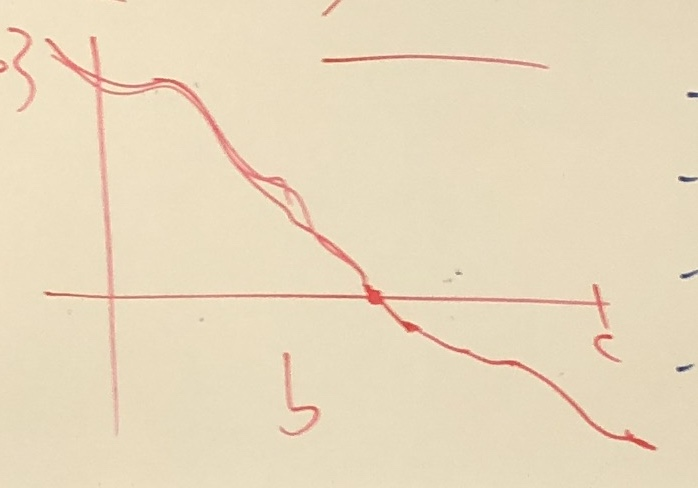
\includegraphics[scale=0.5]{stoch_littlewood}
\caption{Figure for example \ref{stoch.dp.two.class.littewood}.}
\label{stoch_littlewood_fig}
\end{center}
\end{figure}


\end{example}

\begin{example}[\textbf{\(n\)-class capacity allocation}]\label{stoch.dp.n.class.capacity}

\(n\) fare classes: \(P_1 > P_2 > \ldots > P_n\). Demand for class \(i\): \(D_i\), all independent. Sequential arrival of demand. Look at as DP. Let \(x\) be the number of seats remaining. Let \(V_j(x)\) be the max expected seat that can be offered for class \(j\), \(j-1\), \(j-2\), \(\ldots\), 2, 1, given that we have \(x\) seats remaining at the beginning of state \(j\). Goal: compute \(V_n(C)\). Initialization: \(V_1(x) = P_1 \E \min\{x, D_1\}\), 

\[
V_j(x) = \max_{y_{j-1} \leq x} \left\{  \underbrace{P_j \E \left[\min\{D_j, x - y_{j-1}\} \right]  + \E \left[ V_{j+1} \left( \max\{ y_{j-1}, x - D_j \}\right)  \right] }_{W_j(x, y_{j-1})}\right\}
\]

where \(y_{j-1}\) is the amount of seats reserved for class \(j-1, j-2, \ldots, 2, 1\).

\end{example}

\begin{theorem}\label{stoch.dp.n.class.capacity.thm}

For the capacity allocation problem with \(C\) seats (Example \ref{stoch.dp.n.class.capacity}), the optimal booking control policy is given a nested protection level \(y_1^* \leq \ldots \leq y_n^* = C\). (e.g., \(y_2^*\) is the number of seats reserved for class 1 and 2, \(y_3\) is left for 3, 2, and 1, etc. Fixed number independent of remaining capacity.)

\end{theorem}

For ease of exposition, assume demand is continuous (so we can take derivatives. can just use finite differences if you want to be discrete, just a pain.). First we will need a lemma.

\begin{lemma}\label{stoch.dp.n.class.capacity.thm.lemma}

Suppose demand and inventory are continuous. Then for each \(j \geq 1\), 

\begin{enumerate}



\item \(V_j(\cdot)\) is an increasing and concave function.

\item There exist optimal protection levels \(y_j^*\) for \(j \in [n]\) that maximize expected revenue, given by the solutions to \(V_{j-1}' (y_{j-1}^*) = P_j\).

\item \(V_j'(x) \geq V_{j-1}'(x)\) for all \(x\).

\end{enumerate}

\end{lemma}

\begin{proof}

We'll prove that \(V_j(\cdot)\) is an increasing and concave function by induction on \(j\). For \(j=1\), \(V_1(x) = P_1 \E[ \min\{x, D_1\}]\), so it's trivially true. Next, assume that the result holds for \(V_{j-1}(\cdot)\). We'll prove that it's true for \(V_j(\cdot)\). For all \(x \geq y\),

\[
W_j(x, y) = P_j \E \left[\min\{D_j, x - y \} \right]  + \E \left[ V_{j+1} \left( \max\{ y, x - D_j \}\right)  \right], \qquad V_j(x) = \min_{y \leq x} W_j(x,y).
\]

Then

\begin{align*}
\pderiv{}{y} W_j(x,y) & = - P_j \E \left[ \mathbbm{1}\{D_j > x - y\} \right] + \E \left[ V_{j-1}'(y) \cdot \mathbbm{1}\{x - D_j < y \} \right]
\\ & = \mathbb{P}(D_j > x-y) (- P_j + V_{j-1}'(y)). 
\end{align*}

By the inductive hypothesis, \(V_{j-1}(\cdot)\) is concave, so \(- P_j + V_{j-1}'(y)\) is decreasing in \(y\). Notice that \(V_{j-1}'(0) \geq P_{j-1} > P_j\) since \(V_{j-1}'(0)\) is the marginal revenue. Therefore there exists \(y_{j-1}^*\) such that for \(y < y_{j-1}^*\) \(\pderiv{}{y} W_j(x,y) \) is positive and for \(y > y_{j-1}^*\) \(\pderiv{}{y} W_j(x,y) \) is negative. Then

\[
V_j(x) = \max_{y \leq x} W_j(x,y) = W_j(x, \min\{x, y_{j-1}^*\}) 
\]

Then the optimal protection level \(y_{j-1}^*\) for class \(j-1, j-2, \ldots, 2, 1\) is the value such that 

\begin{enumerate}

\item For continuous demand: \(V_{j-1}' (y_{j-1}^*) = P_j\). (notice that this is the same as in the two-class case.)

\item For discrete demand \textbf{(need for Poisson case in homework 2 question 6)}: \(y_{j-1}^* = \max\{y: P_j < \Delta V_{j-1}(y)\}\) where \(\Delta V_{j-1}(y) = V_{j-1}(y) - V_{j-1}(y-1)\).

\end{enumerate}

Consider the continuous case.

\begin{align}
V_j(x) & = W_j(x, \min\{x, y_{j-1}^* \}) 
\\ & = P_j \E [ \min\{D_j, (x - y_{j-1}^*)^+\} ] + \E[ V_{j-1}( \max\{x - D_j, \min\{x, y_{j-1}^*\} \})]
\\ & = \begin{cases}
V_{j-1}(x), & x \leq y_{j-1}^* \\
P_j \E[ \min\{D_j, x - y_{j-1}^*\}] + \E[ V_{j-1}(\max\{x - D_j, y_{j-1}^*\} ) ] , & x \geq y_{j-1}^*
\end{cases}
\\ \implies V_j'(x) & = \begin{cases}
V_{j-1}'(x), & x \leq y_{j-1}^* \\
P_j \E[  \mathbbm{1} \{D_j > x - y_{j-1}^*\}] + \E[ V_{j-1}'(x- D_j) \mathbbm{1}  \{x - D_j > y_{j-1}^*\} ] , & x \geq y_{j-1}^*
\end{cases}\label{stoch.dp.vjprime}
\end{align}

Goal: show \(V_j'(x)\) is decreasing in \(x\). We already know \(V_{j-1}'(x)\) is decreasing in \(x\) by inductive hypothesis. So we focus on the other part (when \(x \geq y_{j-1}^*\)).

\begin{align}
& P_j \E[  \mathbbm{1} \{D_j > x - y_{j-1}^*\}] + \E[ V_{j-1}'(x- D_j) \mathbbm{1}  \{x - D_j > y_{j-1}^*\} ] \nonumber
\\  = \ &    P_j \E[ 1 -  \mathbbm{1} \{D_j < x - y_{j-1}^*\}] + \E[ V_{j-1}'(x- D_j) \mathbbm{1}  \{x - D_j > y_{j-1}^*\} ] \nonumber
\\ = \ &  P_j +  \E \left[ \mathbbm{1} \{D_j < x - y_{j-1}^*\}  (-P_j + V_{j-1}'(x - D_j))\right] \label{stoch.dp.vjprime.exp}
\end{align}

Note for each \(D_j\), the expression inside the expectation operator is nonincreasing in \(x\) (see Figure \ref{stoch_dp_n_class_fig}). So it holds over expectations that \(V_j'(x)\) is nonincreasing in \(x\). Now we want to show that \(V_j'(x) \geq V_{j-1}'(x)\) for all \(x\). Again, it holds trivially that if \(x \leq y_{j-1}^*\) then \(V_j'(x)  = V_{j-1}'(x) \geq V_{j-1}'(x)\), so we focus on the case \(x \geq y_{j-1}^*\). Note that \(\mathbbm{1} \{x - D_j \geq  y_{j-1}^*\}  \geq  \mathbbm{1}\{x \geq y_{j-1}^*\}\) and that since \(V_{j-1}'(\cdot)\) is nonincreasing \( V_{j-1}'(x - D_j) \geq V_{j-1}'(x)\). Then from (\ref{stoch.dp.vjprime.exp})

\begin{figure}[htbp]
\begin{center}
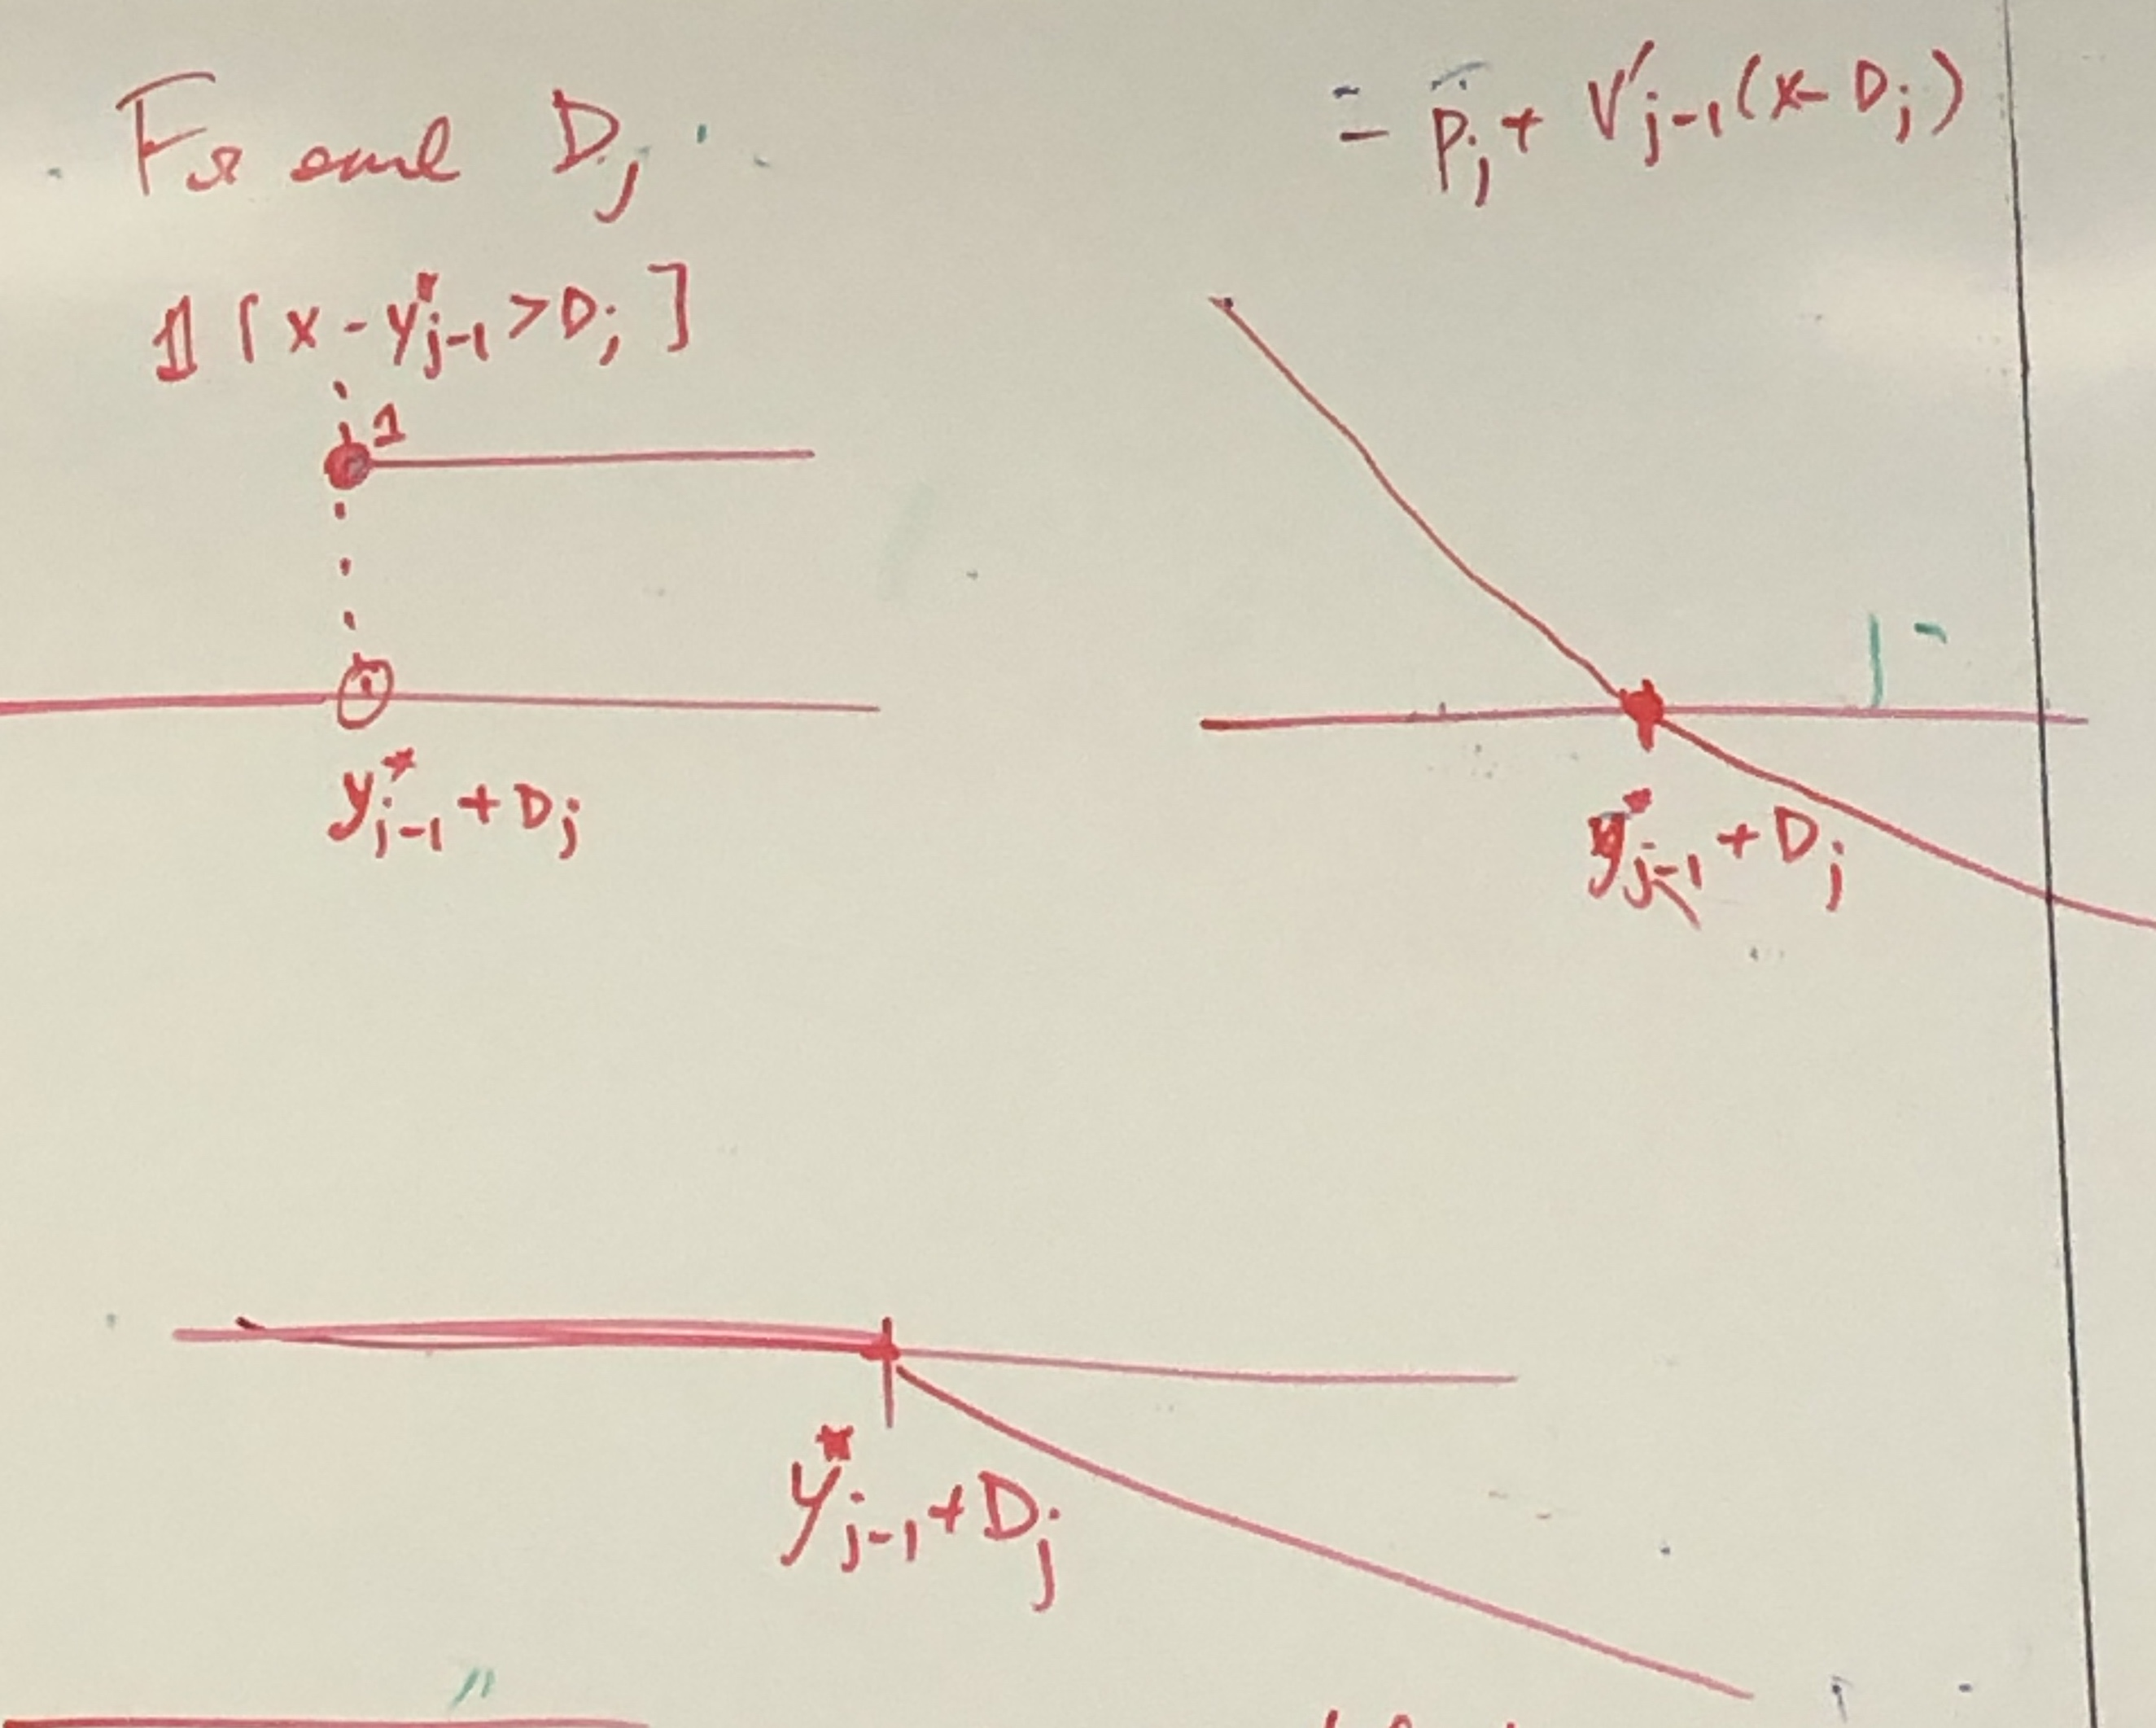
\includegraphics[scale=0.15]{stoch_dp_n_class}
\caption{The argument of the expectation operator in (\ref{stoch.dp.vjprime.exp}) is nonincreasing in \(x\) regardless of the value of the random variable \(D_j\), so the expectation itself is nonincreasing in \(x\).}
\label{stoch_dp_n_class_fig}
\end{center}
\end{figure}




\begin{align*}
V_j'(x) & = P_j +  \E \left[ \mathbbm{1} \{x - D_j \geq  y_{j-1}^*\}  (-P_j + V_{j-1}'(x - D_j))\right] \\
& \geq P_j + \E\left[  \mathbbm{1}\{x \geq y_{j-1}^*\}(- P_j + V_{j-1}'(x) \right] 
\\ & = V_{j-1}'(x).
\end{align*}

%where we plugged in  \(\tilde{x} := x - D_j\).

\end{proof}

Now we can prove the main result.

\begin{proof}[Proof of Theorem \ref{stoch.dp.n.class.capacity.thm}]

It only remains to show that the optimal protection levels are nested. We want to show that \(y_j^* \geq y_{j-1}^*\). From Lemma \ref{stoch.dp.n.class.capacity.thm.lemma} we know that the optimal protection levels are given by \(V_j'(y_j^*) = P_{j+1}\). What does \(V_j'(\cdot)\) look like? It's given in (\ref{stoch.dp.vjprime}). Since \(P_{j} > P_{j+1}\) and per Lemma \ref{stoch.dp.n.class.capacity.thm.lemma} \(V_j'(x) \geq V_{j-1}'(x)\) for all \(x\), it holds that \(y_{j-1}^* < y_j^*\).  See a depiction in Figure \ref{stoch_dp_n_class_pf_fig}.

\begin{figure}[htbp]
\begin{center}
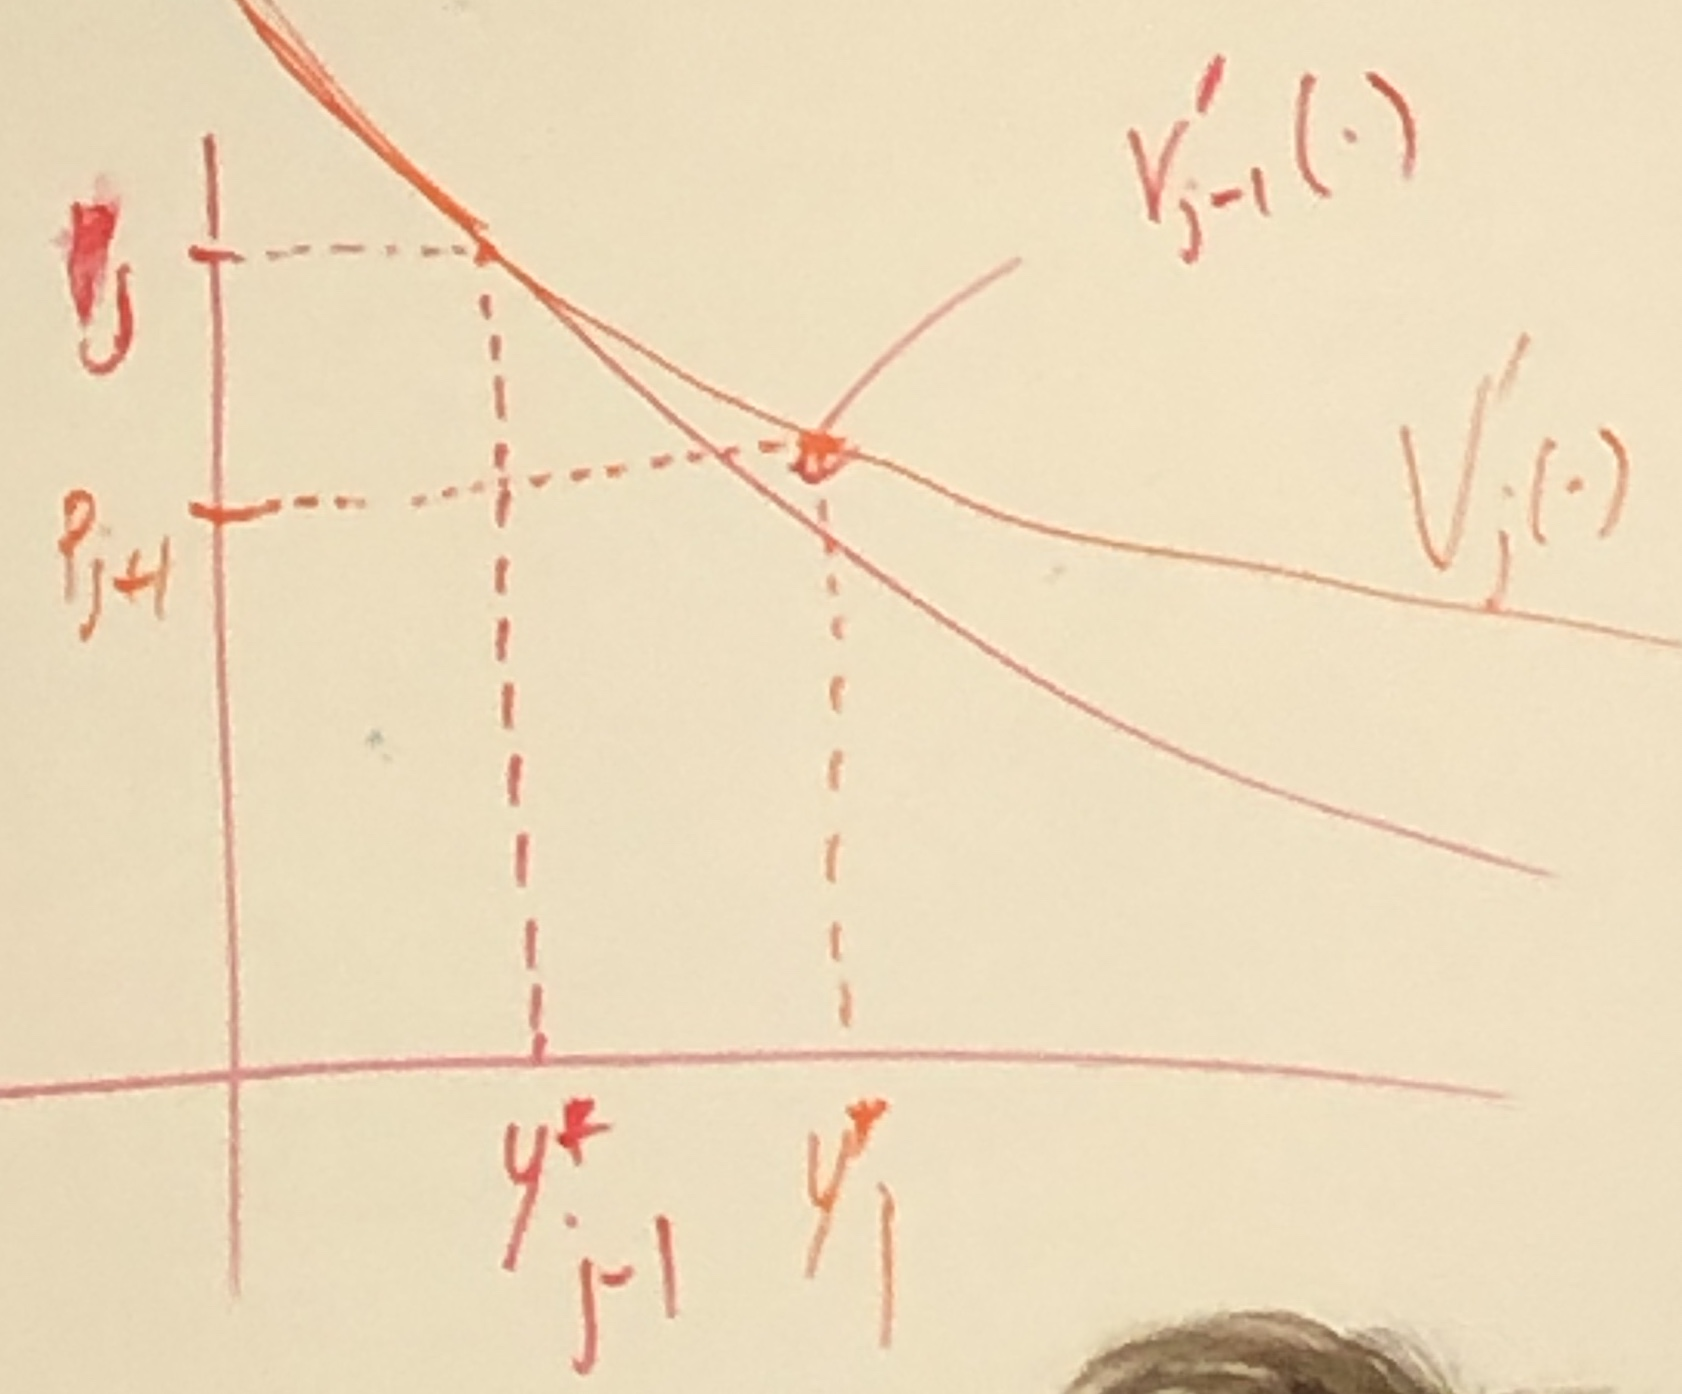
\includegraphics[scale=0.2]{stoch_dp_n_class_pf}
\caption{Illustration of nested protection levels from Theorem \ref{stoch.dp.n.class.capacity.thm}.}
\label{stoch_dp_n_class_pf_fig}
\end{center}
\end{figure}


%By Lemma \ref{stoch.dp.n.class.capacity.thm.lemma},

\end{proof}

\subsection{Optimal Stopping (Section 3.4 of \citet{v1_bertsekas2012dynamic})}

\begin{example}[\textbf{Optimal stopping}]

You own an asset. You are given money \(w_h \geq 0\) in period \(h\). If you accept an offer, you can invest the money at a risk-free rate \(r > 0\). If you reject the offer, you wait for the next one. Assume \(w_0, w_1, \ldots, w_{N-1}\) are independent random variables. Goal: maximize. the total reward (money) at the end of period \(N\).  Now

\[
J_k(x) = \max\left\{ \underbrace{(1+r)^{N-k} x }_{\text{if you stop}} , \underbrace{\E \left[ J_{k+1}(w_k) \right] }_{\text{if you don't stop}} \right\}, \qquad J_N(x) =x.
\]

Optimal policy: stop (accept the current offer) if and only if 

\[
x \geq \frac{\E_{w_k}[J_{k+1}(w_k)]}{(1 + r)^{N-k}} := \underbrace{\alpha_k}_{\text{threshold in period }k}.
\]

\textbf{Claim:} If \(w_0, w_1, \ldots, w_{N-1}\) are i.i.d., then \(\alpha_0 \geq \alpha_1 \geq \ldots \geq \alpha_{N -1}\). 

Let \(V_k(x) := J_k(x)/(1 + r)^{N-k}\). We have \(V_N(x) = x\), 

\[
V_k(x) = \max \left \{x,  \underbrace{\frac{ \E[V_{k+1}(w)] }{1 + r}}_{\text{state independent: no dependence on } x} \right\}.
\]

We'll show that \(V_0(\cdot) \geq V_1(\cdot) \geq \ldots \geq V_{N-1}(\cdot)\). Base case: \(V_{N-1}(x) \geq V_N(x)\), obvious. Next:

Suppose \(V_{k+1}(\cdot) \geq V_{k+2}(\cdot)\). Then 

\begin{align*}
V_k(x) & =  \max \left\{x,  \frac{ \E[V_{k+1}(w)] }{1 + r} \right\}
\\ & \geq \max \left\{x,  \frac{ \E[V_{k+2}(w)] }{1 + r} \right\}
\\ & = V_{k+1}(x).
\end{align*}

\end{example}

\begin{example}[\textbf{Exotic options, optimal stopping}]

Suppose that the price of your asset (option) depends on the prices of \(n = 10\) other assets. So the state is \((x_1, \ldots, x_{10})\). Then

\[
J_k(x_1, \ldots, x_{10}) =  \max\left\{ \underbrace{G(x_1, \ldots, x_{10}) }_{\text{stop now}},   \underbrace{\E \left[ J_{k+1}(\tilde{x}_1, \ldots, \tilde{x}_{10}\right] }_{\text{don't stop now}}\right\}
\]

where \(J_k(x_1, \ldots, x_{10}) \) is the current prices of the 10 assets that influence/determine the value of your ``option" or asset and \(G(x_1, \ldots, x_{10})\) is the reward for selling, and

\[
J_N(x_1, \ldots, x_N) = g(x_1,  \ldots, x_{10}).
\]

Suppose that \(x_i\) takes values \(\{1, \ldots, 100\}\). 

\end{example}

\subsection{Infinite Horizon (Sections 1.2, 1.5 and 2.1 of \citet{v2_bertsekas2012dynamic}; starts on p. 210 of pdf for Volume 3)}\label{statlearning.inf.horizon}

Restatement of setup: infinite horizon problems with discounted cost:

\[
x_{k+1} = f(x_k, u_k, w_k) 
\]

\[
J^*(x_0) = \min_{\pi \in \Pi} \E \left[ \sum_{k=0}^\infty \alpha^k g(x_k, \mu_k(x_k), w_k)  \mid x_0\right]
\]


Stationary discrete-time systems 

\[
x_{k+1} = f(x_k, u_k, w_k), \qquad k \in \{0, 1, \ldots\}
\]

where for all \(k\), \(x_k \in \mathcal{X}\) is the state at time \(k\), \(u_k \in \mathcal{U}\) is the control, and we require \(u_k \in \mathcal{U}(x_k)\) (that is, there is a set of allowable controls given state \(x_k\), and \(w_k \in \mathcal{W}\) are disturbances.

Important: the random disturbances \(w_k: k \in \{0, 1, 2, \ldots\}\) are characterized by a transition probability \(\mathbb{P}(\cdot \mid x_k, u_k)\) that is independent of \(k\). (only dependent on state and control; not time. Nothing indexed by time; assume process is stationary.) Also, \(w_k \indep w_{k-1}, w_{k-2}, \ldots, w_0\).

Given an initial state \(x_0\), we want to find a policy \(\Pi = \{\mu_0, \mu_1, \mu_2, \ldots \}\) where \(\mu_k : \mathcal{X} \to \mathcal{U}\) with \(\mu_k(x_k) \in \mathcal{U}(x_k)\) that minimizes the cost for

\[
J_\pi(x_0) := \underset{N \to \infty}{ \lim \sup} \underset{w_0, w_1, \ldots}{\E} \left[  \sum_{k=0}^N \alpha^k g(x_k, \mu_k(x_k), w_k) \right]
\]

where \(\alpha \in (0,1) \) is the discount factor (typically close to 1).

Let \(\Pi\) be the space of admissible polices. Our goal is to determine an optimal cost function \(J^*: \mathcal{X} \to \mathbb{R}\)

\[
J_k^* = \min_{\pi \in \Pi} J_\pi(x).
\]

Key reason to study infinite horizon problems: in most cases, an optimal policy is stationary: \(\Pi^* = \{\mu, \mu, \mu, \ldots\}\). If the policy is stationary, we write \(J_\mu(\cdot)\) (a policy is a sequence of functions mapping states to actions, but often in this case the policy is stationary, so the sequence is just the same function repeated). A stationary policy is optimal if \(J_\mu(x) = J^*(x)\) for all \( x \in \mathcal{X}\). 

\begin{definition}[\textbf{MDP [Markov decision process] Assumption}]

We assume that the state space \(\mathcal{X}\), the control set \(\mathcal{U}\), and the disturbance space \(\mathcal{W}\) are all finite.



\end{definition}

The MDP assumption corresponds to the classical finite-state Markov decision process. Let \(\mathcal{X} = \{1, \ldots, n\}\). The transition matrix is given by

\[
P_{ij} (u) = \mathbb{P}(X_{k+1} = j \mid X_k = i, U_k = u ).
\]

We can write this using the system dynamics notation as follows:

\[
x_{k+1} = f(x_k, u_k, w_k) = w_k
\]

For each decision \(u\),

\[
W_{ij}(u) = \left\{ w \in \mathcal{W} \mid f(i, u ,w ) = j\right\}, \qquad P_{ij}(u) = \mathbb{P}(W_{ij}(u) \mid i, u).
\]

\begin{example}

\(X = \{1,2\}\), \(U = \{A, B\}\). 

\[
\mathbb{P}_{ij}(u = A) = \begin{pmatrix}
1/2 & 1/2 \\
3/4 & 1/4
\end{pmatrix}, \qquad  \mathbb{P}_{ij}(u = B) = \begin{pmatrix}
1/6 & 5/6 \\
5/6 & 1/6
\end{pmatrix}
\]

Define a random disturbance \(W\) as follows (we need to specify \(\mathbb{P}(W = j \mid i , u)\)):

\[
\mathbb{P}(W = j \mid i, u) = \begin{cases}
 1/2  \text{ for } j=1, \qquad 1/2 \text{ for } j = 2   & \text{if } i = 1, u = A \\
 3/4 \text{ for } j=1, \qquad 1/4 \text{ for } j = 2   & \text{if } i = 2, u = A \\
  1/6 \text{ for } j=1, \qquad 5/6 \text{ for } j = 2   & \text{if } i = 1, u = B \\
 5/6 \text{ for } j=1,\qquad  1/6 \text{ for } j = 2   & \text{if } i = 2, u = B \\
\end{cases}
\]

\end{example}

Given the MDP assumption, 2 key questions.

\begin{enumerate}

\item Does the optimal cost \(J^*\) satisfy some kind of Bellman equation?

\item How do we compute the optimal policy?

\end{enumerate}

\textbf{Motivation for the Bellman Equations}

\(J^*(x)\) is the optimal cost function (stationary). Will satisfy (guess, will prove)

\[
J^*(x) = \min_{u \in \mathcal{U}(x)} \left\{ \E[g(x,u,w) ] + \alpha \E \left[ J^*(f(x,u,w)) \right] \right\}
\]

Consider an arbitrary policy \(\pi = \{\mu_0, \mu_1, \mu_2, \ldots\}\). Suppose we consider the cumulative cost of the first \(n\) states and add some terminal cost \(\alpha^n J(x_n)\). The expected total cost is 

\[
\underset{w_0, \ldots, w_{n-1}}{\E} \left[ \alpha^n J(x_n) + \sum_{k=0}^{n-1} \alpha^k g(x_h, \mu_h(x_h), w_k) \right]
\]

Suppose we want to find the minimum cost of \(N\) states \(H_N(x), \alpha^N J(x)\). For \(h \in \{1, 2, \ldots, N\}\),

\[
H_{n-h}(x) = \min_{u \in \mathcal{U}(x)} \underset{w}{\E} \left[ \alpha^{N-h} g(x, u, w) + H_{n-h+1}(f(x,u,w)) \right].
\]

\[
\iff H_{n-h-1}(x) = \min_{u \in \mathcal{U}(x)} \underset{w}{\E} \left[ \alpha^{N-h-1} g(x, u, w) + H_{n-h}(f(x,u,w)) \right].
\]

let \(V_k(x) := \frac{H_{n-k}(x)}{\alpha^{N-k}}\). Then we have the following DP algorithm:

\[
V_0(x) = J(x); \qquad V_{k+1}(x) = \min_{u \in \mathcal{U}(x)} \underset{w}{\E} \left[ g(x, u, w) + \alpha V_k(f(x,u,w0)\right] 
\]

Intuition: \(V_k(x)\) is the minimum net present value of the cost of an \(h\)-stage problem given that we start in state \(X\). 

\begin{definition}

A dynamic programming operator \(T: \mathbb{R}^{|\mathcal{X}|} \to \mathbb{R}^{|\mathcal{X}|}\) is defined as follows: given \(J: \mathcal{X} \to \mathbb{R}\), with \(J \in \mathbb{R}^{|\mathcal{X}|}\), for all \(x \in \mathcal{X}\), \(TJ \in \mathbb{R}^{|\mathcal{X}|}\) where

\[
(TJ)(x) := \min_{u \in \mathcal{U}(x)} \left\{ \underset{w}{\E} \left[ g(x,u,w) + \alpha J(f(x,u,w)) \right] \right\}
\]

\end{definition}

Important observation: \(TJ\) is the optimal cost for a one stage problem that has a state cost \(g\) and a terminal cost \(\alpha J\).

Similarly, for any stationary policy \(\mu: \mathcal{X} \to \mathcal{U}\) and \(J: \mathcal{X} \to \mathbb{R}\) define \(T_\mu: \mathbb{R}^{|\mathcal{X}|} \to \mathbb{R}^{|\mathcal{X}|}\) such that for all \(x \in \mathcal{X}\)

\[
(T_\mu J)(x) := \E \left[ g(x,\mu(x) ,w) + \alpha J(f(x,\mu(x),w)) \right] 
\]

Notation: \(T^k = T \circ T \circ \ldots \circ T\). \(T_k\) is the optimal cost for the \(k\)-stage \(\alpha\)-discounted problem with an initial state \(x\), cost-per-state \(g\), and terminal cost \(\alpha^k J\).

Note; if \(\Pi = \{\mu_0, \ldots, \mu_{k-1}\}\), then the cost of the policy \(\Pi\) for the \(k\)-stage problem with initial state \(x\), cost-per-state \(g\), and terminal cost \(\alpha^k J\) is \((T_{\mu_0} T_{\mu_1} \cdots T_{u_{k-1}} J)(x)\). 

One last remark: since typically \(g(x,u,w) \geq 0\), we have the inequality

\begin{equation}\label{stoch.dp.operator.ineq}
(TJ)(x) \leq \alpha J(f(x,u,w)) .
\end{equation}

\begin{definition}[\textbf{Contraction Mapping (Section 1.5 of \citet{v2_bertsekas2012dynamic})}]\label{statlearning.def.contraction}

Let \((Y, \lVert \cdot \rVert)\) be a real normed vector space. A function \(T: Y \to Y\) is said to be a \textbf{contraction mapping} if. for some \(\alpha \in (0,1)\), we have

\[
\lVert Ty - Tz \rVert \leq \alpha \lVert y - z \rVert, \qquad \forall y \in Y.
\]

The scalar \(\alpha\) is said to be the \textbf{modulus of contraction} of \(T\).

(See also Definition \ref{ra.def.contraction}. For more on contraction mappings, see Section \ref{ra.contractions.odes}.)

\end{definition}




If \(Y\) is a Banach space (that is, complete under the norm \(\lVert \cdot \rVert\)), a contraction mapping \(F: Y \to Y\) has a unique fixed point; that is, the equation \(y = Fy\) has a unique solution \(y^*\) called the \textbf{fixed point} of \(F\). Further, the sequence \(\{y_k\}\) generated by the iteration \(y_{k+1} = F y_k\) converges to \(y^*\) starting from an arbitrary initial point \(y_0\).

We will want to show that the dynamic programming operator is a contraction mapping. It will be enough to show that the dynamic programming operator is \textbf{monotonic} and has \textbf{constant shift.}

\begin{theorem}[\textbf{Blackwell's Sufficient Conditions}]\label{dp.blackwell.sc}

Let \(\mathbb{R}^{|X|}\) be a space of bounded functions \(J: X \to \mathbb{R}\) with the sup metric. Let \(T: \mathbb{R}^{|X|} \to \mathbb{R}^{|X|}\) be an operator satisfying two conditions:

\begin{enumerate}

\item \textbf{(Monotonicity)} If \(J, J' \in \mathbb{R}^{|X|}\) and \(J(x) \leq J'(x)\) for all \(x \in X\), then \((TJ)(x) \leq (TJ')(x)\) for all \(x \in X\).

\item \textbf{(Discounting)} There exists \(\alpha \in (0,1)\) such that 

\[
(T(J + c))(x) \leq (TJ)(x) + \alpha c \qquad \forall J \in \mathbb{R}^{|X|}, c \geq 0, x \in X.
\]

\end{enumerate}

Then \(T\) is a contraction mapping with modulus \(\alpha\).

\end{theorem}

\begin{proof}

Let \(J, J' \in \mathbb{R}^{|X|}\). Then

\[
J(x) = J'(x) + J(x) - J'(x) \leq J'(x) + \sup_{y \in X} \left| J(y) - J'(y) \right| = J'(x) + \lVert J - J' \rVert_\infty, \qquad \forall x \in X,
\]

which we can write in shorthand as

\[
J \leq J' + \lVert J - J' \rVert_\infty.
\]

Properties (1) and (2) imply that for some \(\alpha \in (0,1)\)

\begin{multline*}
TJ \leq T(J' + \lVert J - J' \rVert_\infty) \leq TJ' +  \alpha \lVert J - J' \rVert_\infty \qquad \iff TJ- TJ' \leq \alpha \lVert J - J' \rVert_\infty,  
\\ TJ' \leq T(J + \lVert J - J' \rVert_\infty) \leq TJ +  \alpha \lVert J - J' \rVert_\infty \qquad \iff TJ' - TJ \leq \alpha \lVert J - J' \rVert_\infty.
\end{multline*}

Combining these, we have

\begin{multline*}
 \left| (TJ)(x) - (TJ')(x)  \right|  \leq \alpha \lVert J - J' \rVert_\infty \qquad \forall x \in X
\\ \implies \qquad \sup_{x \in X} \left|  (TJ)(x) - (TJ')(x) \right|  \leq \alpha  \lVert J - J' \rVert_\infty \
\\ \implies \lVert TJ - TJ' \rVert_\infty \leq \alpha \lVert J - J' \rVert_\infty.
\end{multline*}

\end{proof}

Now we will show that these properties hold.




 
 


\begin{theorem}[\textbf{Properties of \(T\) and \(T_\mu\)}]\label{dp.thm.dp.op.mono.cs}

\begin{enumerate}

\item

\textbf{Monotonicity: (Lemma 1.1.1 in \citet{v2_bertsekas2012dynamic}, p.9)} for any \(J: \mathcal{X} \to \mathbb{R}\) and \(J': \mathcal{X} \to \mathbb{R}\) such that \(J(x) \leq J'(x)\) for all \(x \in \mathcal{X}\), then

\[
(T^kJ)(x) \leq (T^k J')(x), \qquad (T_\mu^k J)(x) \leq (T_\mu^k J')(x).
\]

for any \(k \geq 0 \).

\item \textbf{Constant shift  (Lemma 1.1.2 in \citet{v2_bertsekas2012dynamic}, p. 9):} For each \(k \geq 0\),  \(J: \mathcal{X} \to \mathbb{R}\) and scalar \(r\),

\[
[T^k (J + r \boldsymbol{e})](x) = (T^kJ)(x) + \alpha^k r, \qquad  [T_\mu^k (J + r \boldsymbol{e})](x) = (T_\mu^kJ)(x) + \alpha^k r, 
\]

where \(\boldsymbol{e}\) is a vector of all 1s.

%\item \textbf{Contraction mapping.}

\end{enumerate}

\end{theorem}

\begin{proof}[Proof of monotonicity (Lemma 1.1.1 in \citet{v2_bertsekas2012dynamic})]

\end{proof}

\begin{proof}[Proof of constant shift (Lemma 1.1.2 in \citet{v2_bertsekas2012dynamic})]

\end{proof}



Now we can show that the dynamic programming operator is a contraction mapping.

\begin{theorem}[\textbf{Proposition 1.2.6 in \citet{v2_bertsekas2012dynamic}}] \label{dp.op.c.mapping}

 The dynamic programming operator \(T\) is a contraction mapping in the normed vector space \((\mathbb{R}^{|X|}, \lVert \cdot \rVert_\infty)\) (where \( \lVert J \rVert_\infty = \sup_{x \in \mathcal{X}}|J(x)|\)).

\end{theorem}

\begin{proof}

Theorem \ref{dp.thm.dp.op.mono.cs} shows that the sufficient conditions of Theorem \ref{dp.blackwell.sc} are satisfied for the dynamic programming operator \(T\).

%We need to show that for any \(J : \mathcal{X} \to \mathbb{R}\) and \(J': \mathcal{X} \to \mathbb{R}\),
%
%\[
%\left\lVert TJ - TJ' \right \rVert_\infty \leq \alpha \left\lVert J - J' \right \rVert_\infty
%\]
%
%We will use the fact that \((TJ)(x) \geq 0\).
%
%\begin{align*}
%|(TJ)(x) - (TJ')(x)| & = \left| \min_{u \in \mathcal{U}(x)} \left\{ \E \left[ g(x,u,w) + \alpha J(f(x,u,w)) \right] \right\} - \min_{u \in \mathcal{U}(x)} \left\{ \E \left[ g(x,u,w) + \alpha J'(f(x,u,w)) \right] \right\} \right|
%%\\ & \leq \left| \min_{u \in \mathcal{U}(x)} \left\{ \E \left[ g(x,u,w) \right] + \E \left[ \alpha J(f(x,u,w)) \right]  -\E \left[ g(x,u,w) \right] -  \E \left[ \alpha J'(f(x,u,w)) \right] \right\} \right|
%%\\ & = \left| \min_{u \in \mathcal{U}(x)} \left\{  \E \left[ \alpha J(f(x,u,w)) \right]   -  \E \left[ \alpha J'(f(x,u,w)) \right] \right\} \right|
%\\ & \leq\min_{u \in \mathcal{U}(x)}  \left\{   \left|  \alpha \E \left[  J(f(x,u,w)) \right]   -  \alpha  \E \left[ J'(f(x,u,w)) \right] \right| \right\} 
%\\ & = \min_{u \in \mathcal{U}(x)}  \left\{ \alpha  \left|  \E \left[  J(f(x,u,w)) - J'(f(x,u,w)) \right] \right| \right\}
%\\ & \leq  \alpha  \min_{u \in \mathcal{U}(x)} \E  \left|    J(f(x,u,w)) - J'(f(x,u,w)) \right| \text{ (by Jensen's inequality)}
%\end{align*}

\end{proof}

(For more on contraction mappings, see Section \ref{ra.contractions.odes}.)

3 questions to prove (similar to Proposition 7.2.1, p. 214 of pdf of 3rd edition):

\begin{enumerate}

\item \textbf{Convergence of DP algorithm (second part of Proposition 1.5.1 in \citet{v2_bertsekas2012dynamic}, p. 48; second part of Proposition 1.5.4, p. 53):} under the MDP assumption, for every \(J : \mathcal{X} \to \mathbb{R}\) and for any policy \(\mu: \mathcal{X} \to \mathcal{U}\), \(J^* = \lim_{k \to \infty} T^kJ, \qquad J_\mu = \lim_{h \to \infty} T_\mu^h J\).

note that

\[
(TJ^*)(x) = \min_{u \in \mathcal{U}(x)} \left\{ \E \left[ g(x,u,w) + \alpha J^*(f(x,u,w)) \right] \right\} = J^*(x).
\]

Statement in book: If \(T: \mathbb{R}^{|X|} \to \mathbb{R}^{|X|}\) is a contraction mapping with modulus \(\alpha \in (0,1)\), then \(\{T^k J\}\) converges to \(J^*\) for any \(J \in \mathbb{R}^{|X|}\), and we have

\[
\lVert T^k J - J^* \rVert \leq \alpha^k \lVert J - J^* \rVert, \qquad k \in \mathbb{N}.
\]

\textbf{notes from review on 2/11/10:} \(J^*\) is the unique fixed point of \(T\) and \(J_\mu\) is the unique fixed point of \(T_\mu\) and \(J^* = \lim_{k \to \infty} T^k J\) (used contraction mapping to prove).

\item \textbf{Bellman's equations (first part of Proposition 1.5.1 in \citet{v2_bertsekas2012dynamic}, p. 48; first part of Proposition 1.5.4, p. 53).} The optimal cost \(J^*\) is the unique solution to the equation

\begin{equation}\label{stoch.dp.bellman.eqn.infinite.horizon}
J^*(x) = \min_{u \in \mathcal{U}(x)} \left\{ \E \left[ g(x,u,w) + \alpha J^*(f(x,u,w)) \right]\right\}
\end{equation}

That is, \(J^* = T J^*\). (Statement in book: ``If \(T: \mathbb{R}^{|X|} \to \mathbb{R}^{|X|}\) is a contraction mapping with modulus \(\alpha \in (0,1)\), then there exists a unique \(J^* \in \mathbb{R}^{|X|}\) such that \(J^* = TJ^*\).")

Similarly, for any stationary policy \(\mu: \mathcal{X} \to \mathcal{U}\), the cost associated with \(\mu\) is the unique solution to the following equation:

\[
J_\mu(x) = \E\left[  g(x,\mu(x),w) + \alpha J_\mu(f(x,\mu(x) ,w)) \right]
\]

That is, the only solution to the system of \(n = | \mathcal{X}|\) equations \(TJ = J\) is optimal.


\item \textbf{Optimal control.} A stationary policy \(\mu^*\) is optimal if and only if \(\mu^*(x)\) attains the minimum on the right hand side of the Bellman equation (\ref{stoch.dp.bellman.eqn.infinite.horizon}). 

\[
T_{\mu^*} J^* = T J^* \iff J_{\mu^*} = J^*.
\]

\end{enumerate}


%\begin{proposition}[\textbf{Convergence of DP Algorithm; Proposition 1.5.1 in \citet{v2_bertsekas2012dynamic}, p. 48)}]\label{dp.prop.1.5.1}
%
%If \(F: \mathbb{R}^{|X|} \to \mathbb{R}^{|X|}\) is a contraction mapping with modulus \(\alpha \in (0,1)\), then \(\{F^k J\}\) converges to \(J^*\) for any \(J \in \mathbb{R}^{|X|}\), and we have
%
%\[
%\lVert F^k J - J^* \rVert \leq \alpha^k \lVert J - J^* \rVert, \qquad k \in \mathbb{N}.
%\]
%
%\end{proposition}


\begin{proof}[Proof of convergence of DP algorithm]

Want to show: consider an arbitrary \(J\). Consider the sequence \(\{T^kJ; k =0,1, \ldots\}\); want to show is Cauchy. For any \(m > 0\), want to show

\[
\lVert J_{m+k} - J_k \rVert_\infty < \epsilon.
\]

We have

\begin{align*}
\lVert J_{m+k} - J_k \rVert_\infty & = \left\lVert  \sum_{i=1}^m( J_{k+i} - J_{k+i-1} )\right\rVert_\infty
\\ & \leq  \sum_{i=1}^m \left\lVert J_{k+i} - J_{k+i-1} \right\rVert_\infty
\\ & \leq  \sum_{i=1}^m \alpha^{k+i-1}  \left\lVert J_{1} - J_{0} \right\rVert_\infty \qquad \text{(by Theorem \ref{dp.op.c.mapping})} 
\\ & =  \left\lVert  J_{1} - J_{0} \right\rVert_\infty \alpha^k  \sum_{i=1}^m \alpha^{i-1}  
\\ & \leq \frac{\left\lVert  J_{1} - J_{0} \right\rVert_\infty\alpha^k }{1 - \alpha}
\end{align*}

since by Theorem \ref{dp.op.c.mapping}

\begin{align*}
\lVert J_{\ell + 1} - J_\ell \rVert_\infty & = \lVert TJ_{\ell} -T J_{\ell - 1} \rVert_\infty
\\ & \leq \alpha \lVert J_\ell - J_{\ell - 1} \rVert_\infty
\\ & \leq \alpha^2 \lVert J_{\ell - 1} - J_{\ell - 2} \rVert_\infty
\\ & \vdots
\\ & \leq \alpha^\ell \lVert J_{1} - J_{0} \rVert_\infty
\end{align*}

Therefore \(\{T^k J: k \geq 0\}\) is Cauchy, and complete. So \(\lim_{h \to \infty} T^kJ\) is well-defined. 



\end{proof}

By definition of \(T^kJ\) and the MDP assumption, the limit is the optimal cost \(J^* = \lim_{k \to \infty} T^k J\).

\begin{proof}[Proof of statement about Bellman's Equation]

Want to prove: \(J^*\) is the unique solution to the Bellman equation (\ref{stoch.dp.bellman.eqn.infinite.horizon}). First we will show it is a solution. For any \(J: \mathcal{X} \to \mathbb{R}\),

\[
\lim_{h \to \infty} T^k J = J^*.
\]

So it must be that \(TJ^* = J^*\) or else convergence is violated. Therefore \(J^*\) is a solution to the Bellman equation. 

Suppose there exists \(J' \neq J^*\) such that \(TJ' = J'\). Then \(T^3 J' = T^2 J' = TJ' = J'\), \(T^k J' = J'\) for all \(k\). then \textbf{???}

\end{proof}

\begin{proof}[Proof of statement about Optimal control]

Suppose that \(TJ^* = T_\mu J^*\). Want to show that \(J^* = J_\mu\). 

\[
J^* = T J^* \text{ (by convergence of DP algorithm)} = T_\mu J^* \text{ (by hypothesis)}
\]

So \(J^*\) is a fixed point of \(T_\mu\). By (2) \(T_\mu\) has a unique fixed point given by \(J_\mu\). Therefore \(J^* = J_\mu\).

Now suppose \(J^* = J_\mu\). Want to show: \(TJ^* = T_\mu J^*\).

\[
J^* = J_\mu \iff T_\mu J^* = T_\mu J_\mu = J_\mu \text{ (by 2)} = J^* \text{ (by hypothesis)} = T J^* \text{ (by 1)}
\]

\end{proof}


Optimality control using matrix notation: Let \(X = \{1, \ldots, n\}\). \(p_{ij}(u) = \mathbb{P}(X_{k+1} = j \mid X_k = i, u_k = u)\).

\begin{align*}
(TJ)(i) & = \min_{u \in \mathcal{U}(i)} \E\left[g(i, u, w) + \alpha J(f(i,u,w)) \right]
\\ & = \min_{u \in \mathcal{U}(i)} \sum_{j=i}^n P_{ij}(u)   \left[g(i, u, j) + \alpha J(j) \right]
\\ & = \min_{u \in \mathcal{U}(i)} \sum_{j=i}^n P_{ij}(u) g(i, u, j)   + \alpha  \sum_{j=i}^n P_{ij}(u) J(j)
\\ \implies TJ(i)  & =  \min_{u \in \mathcal{U}(i)} \overline{g}(i,u)   + \alpha  \begin{bmatrix} \underbrace{P(u)}_{n \times n \text{ matrix}} \underbrace{J}_{n \times 1 \text{ vector}} \end{bmatrix} _i
\\ \iff \underbrace{TJ}_{n \times 1 \text{ vector}}  & = \underbrace{ \begin{bmatrix} \min_{u \in \mathcal{U}(i)} \overline{g}(i,u)  \end{bmatrix}}_{n \times 1 \text{ vector}} + \alpha  \begin{bmatrix} \underbrace{P(u)}_{n \times n \text{ matrix}} \underbrace{J}_{n \times 1 \text{ vector}} \end{bmatrix}
\end{align*}

Question; given a stationary policy \(\mu\), how do I compute \(J \mu\)?

\[
(T_\mu J)(i) = \overline{g}(i,\mu(i) )  + \alpha J(j)  \sum_{j=i}^n P_{ij}(\mu (i)) J(j)
\]

Denote \(J\) as an \(n\)-vector, likewise with \(TJ\). Denote

\[
P_\mu = \begin{pmatrix}
P_{11}(\mu(1)) & P_{12}(\mu(1)) & \cdots & P_{1n}(\mu(1))  \\
P_{21}(\mu(2)) & P_{22}(\mu(2)) & \cdots & P_{2n}(\mu(2))  \\
\vdots & \vdots & \ddots & \vdots \\
P_{n1}(\mu(n)) & P_{n2}(\mu(n)) & \cdots & P_{nn}(\mu(n)) 
\end{pmatrix}
\]

where for example \( P_{12}(\mu(1))\) is the probability that if i have policy \(\mu\) and I'm in state \(1\) I will transition to state 2. And

\[
\overline{g}_\mu = \begin{pmatrix}
\overline{g}(1, \mu(1)) \\
\vdots \\
\overline{g}(n, \mu(n))
\end{pmatrix}
\]

Then \(T_\mu J = \overline{g}_\mu + \alpha P_\mu J\). \(J_\mu\) is the unique fixed point of \(T_\mu\). 

\begin{align*}
T_\mu J_\mu &  = J_\mu
\\ J_\mu & = \overline{g}_\mu + \alpha P_\mu J_\mu
\\ J_\mu & = (I - \alpha  P_\mu)^{-1} g_\mu
\end{align*} 

although this is a bad way to compute because if \(\alpha\) is large (e.g. 0.9999), matrix could be very ill-conditioned since largest eigenvalue of a transition matrix is 1.

\subsection{Value Iterations and Policy Iterations (Sections 2.2 and 2.3 of \citet{v2_bertsekas2012dynamic}; starts on p. 210 of pdf for Volume 3)}

Question: how do I compute \(J^*\) and the optimal policy?

\begin{enumerate}

\item \textbf{VI: value iteration} (also called successive approximation)

Pick \(k_0\) and start with some \(J_0\), apply the DP operator \(T\) \(k_0\) times, output \(T^{k_0} J_0 = \hat{J}\), use \(\hat{J}\) as an approximation for \(J^*\), find a policy (``greedy policy") \(\mu\) such that \(T \hat{J} = T_\mu \hat{J}\). Recall

\[
(T\hat{J})(x) = \min_{u \in \mathcal{U}(x)} \left\{ \E \left[ g(x,u,w) + \alpha \hat{J}(f(x,u,w)) \right] \right\}
\]

Questions: 

\begin{enumerate}

\item

how should we pick \(k\)? (need error bound.) 

\item What is the difference between \(J_\mu\) and \(J^*\)? Want to show: if \(\hat{J}\) is close to \(J^*\), then \(J_\mu\) is also close to \(J^*\). (cost of your policy in practice will be close to optimal.) Important distinction: \(\hat{J} \neq J_{\mu_k}\) (\(\hat{J}\) may not be achievable by any policy, let alone a stationary policy). 

\end{enumerate}

First question: trivial error bound: recall

\[
\lVert T^k J - J^* \rVert_\infty  =  \lVert T^k J -  T^k J^* \rVert_\infty  \leq \alpha^k \lVert J - J^* \rVert_\infty
\]

(see also Equation (7.9) in Bertsekas 3rd edition Vol. 1, p. 215 of pdf)


\begin{theorem}[\textbf{Similar to Proposition 2.2.1 in \citet{v2_bertsekas2012dynamic}; in equation 7.17 (p. 216 of pdf) and 7.23 (p. 219 of pdf) in Bertsekas 3rd edition Vol. 1}]


Monotonic error bound: for any vector \(J\) and state \(i\) with \(k \geq 0\),

\[
(T^k J)(i) + \underline{c}_k \leq (T^{k+1} J)(i) + \underline{c}_{k+1} \leq J^*(i) \leq (T^{k+1}J)(i) + \overline{c}_{k+1} \leq (T^k J)(i) + \overline{c}_k
\]

where

\[
\underline{c}_k = \frac{\alpha}{1-\alpha} \min_{i \in [n]} \left\{ (T^k J)(i) - (T^{k-1}J)(i)  \right\}, \qquad \overline{c}_k = \frac{\alpha}{1-\alpha} \max_{i \in [n]} \left\{ (T^k J)(i) - (T^{k-1}J)(i)  \right\}
\]

\end{theorem}

So when gap between \(\underline{c}_k \) and \(\overline{c}_k \) is small, you know you are close to converging (because as \(k\) increases we know that value converges, so eventually the difference over which you are maximizing and minimizing goes to 0.) 

\begin{proof}

We will only prove the lower bound (the proof of the upper bound is analogous). Let \(\underline{\gamma}_{1} := \min_{i \in [n]} \{ (TJ)(i) - J(i)\}\). Then if \(\boldsymbol{e}\) is the selection vector for the index of this minimum,

\begin{align*}
\underline{\gamma}_{1}\boldsymbol{e}& \preceq TJ - J  
\\ \iff J + \underline{\gamma}_{1}\boldsymbol{e} &  \preceq TJ \qquad 
\end{align*}

where \( \preceq\) denotes an element-wise vector inequality. Next recall from (\ref{stoch.dp.operator.ineq}) that \(TJ \preceq \alpha J\), so \(T \underline{\gamma}_{1}\boldsymbol{e} \preceq \alpha \underline{\gamma}_{1}\boldsymbol{e}\). Therefore we have from the above that \(TJ + \alpha \underline{\gamma}_{1}\boldsymbol{e} \preceq TJ +  T \underline{\gamma}_{1}\boldsymbol{e} \preceq TJ\). It also follows trivially from the above that \(J + \underline{\gamma}_{1}\boldsymbol{e}  + \alpha \underline{\gamma}_{1}\boldsymbol{e}    \preceq TJ  + \alpha \underline{\gamma}_{1}\boldsymbol{e}  \), so we have

\begin{align*}
\\ \iff J + (1  + \alpha) \underline{\gamma}_{1}\boldsymbol{e}\preceq  TJ + \alpha \underline{\gamma}_{1}\boldsymbol{e}& \preceq T^2 J 
\\ \iff J + (1  + \alpha + \alpha^2) \underline{\gamma}_{1}\boldsymbol{e}\preceq TJ + \alpha (1  + \alpha) \underline{\gamma}_{1}\boldsymbol{e}\preceq  T^2J + \alpha^2 \underline{\gamma}_{1}\boldsymbol{e}& \preceq T^3 J 
\end{align*}

Applying this repeatedly yields
\begin{align*}
J + \left( \sum_{i=0}^k \alpha^i  \right) \underline{\gamma}_{1}\boldsymbol{e}& \preceq TJ +  \left( \sum_{i=1}^k \alpha^i  \right) \underline{\gamma}_{1} e
\\ & \preceq T^2J +  \left( \sum_{i=2}^k \alpha^i  \right) \underline{\gamma}_{1} e
\\ & \vdots
\\ & \preceq T^{k+1} J 
\end{align*}

Take the limit as \( k \to \infty\):

\[
J + \underline{\gamma}_{1} \frac{\boldsymbol{e}}{1 - \alpha} \preceq TJ + \frac{\alpha}{1 - \alpha} \underline{\gamma}_{1}\boldsymbol{e}\preceq T^2 J + \frac{\alpha^2}{1 - \alpha} \underline{\gamma}_{1}\boldsymbol{e}\preceq \ldots \preceq T^k J + \frac{\alpha^k \boldsymbol{e}}{1 - \alpha} \preceq \ldots \preceq J^*.
\]

Recall: 

\[
\underline{c}_1 = \frac{\alpha}{1 - \alpha} \min_{i \in [n]} \left\{ (TJ)(i) - J(i) \right\} = \frac{\alpha}{1- \alpha}  \underline{\gamma}_{1}
\]

\begin{equation}\label{stoch.dp.2.2.1.ineq}
\implies J + \frac{\underline{c}_1}{\alpha}\boldsymbol{e}\preceq TJ + \underline{c}_1\boldsymbol{e}\preceq T^2 J + \alpha \underline{c}_1\boldsymbol{e}\preceq  \ldots \preceq T^k J + \alpha^{k-1} \underline{c}_1\boldsymbol{e} \preceq \ldots \preceq J^*,
\end{equation}

%so we have in particular
%
%\[
% \implies J + \frac{\underline{c}_1}{\alpha}\boldsymbol{e}\leq  TJ + \underline{c}_1 \boldsymbol{e} \leq J^*.
% \]
 
Continuing further, since \(J\) is arbitrary, take \(J = T^kJ\). Then re-do analysis with \(J = T^k J\). Then using
\[
\underline{\gamma}_{k+1} = \min(T^{k+1}J)(i) - (T^kJ)(i) = \underline{c}_{k+1} \left(  \frac{1-\alpha}{\alpha} \right)
\]

and the same argument will yield 


\begin{equation}\label{stoch.dp.2.2.1.ineq2}
T^k J + \frac{\underline{c}_{k+1}}{\alpha}\boldsymbol{e} \preceq T^{k+1}J + \underline{c}_{k+1}\boldsymbol{e} \preceq J^*.
\end{equation}

Next, we will show that
$$
\alpha \min_{i \in [n]} \{ (TJ)(i) - J(i)\} ~\leq~ \min_{i \in [n]} (T^2J)(i) - (TJ)(i) 	
$$
Note that, by definition of $\underline{c}_1$ and $\underline{c}_2$, proving the above inequality is equivalent to showing that $\alpha \underline{c}_1 \leq \underline{c}_2$. We have from (\ref{stoch.dp.2.2.1.ineq}) that

%By Equation (\ref{eq:main1}), we have that
\begin{align*}
	T J  + \underline{c}_1 \bm{e}  \preceq T^2 J  + \alpha \underline{c}_1 \bm{e}
	&\qquad \stackrel{}{\Longleftrightarrow}\qquad
	(1-\alpha) \underline{c}_1 \bm{e} ~\preceq~ T^2 J - T J\\
	&\qquad \stackrel{}{\Longleftrightarrow} \qquad
	(1-\alpha) \underline{c}_1  ~\leq~ \min_{i = 1, \ldots, n}    (T^2 J)(i) - (T J)(i)\\
		&\qquad \stackrel{}{\Longleftrightarrow} \qquad
	(1-\alpha) \underline{c}_1  ~\leq~  \frac{1-\alpha}{\alpha} \underline{c}_2\\
			&\qquad \Longleftrightarrow \qquad
	\alpha  \underline{c}_1  ~\leq~ \underline{c}_2
\end{align*}
%where (a) follows because the previous inequality is an inequality between {\bf two vectors}, and thus, the inequality must hold for each component of the vector, and (b) follows from the definition of $\underline{c}_2$.

Then since from (\ref{stoch.dp.2.2.1.ineq})
$T J  + \underline{c}_1 \bm{e}  \preceq T^2 J  + \alpha \underline{c}_1 \bm{e}$ and $\alpha \underline{c}_1 \leq \underline{c}_2$, it follows that \(T J  + \underline{c}_1 \bm{e}  ~\leq~ T^2 J  + \underline{c}_2 \bm{e} ~\leq~ J^*~.\) By a similar argument generalizing from (\ref{stoch.dp.2.2.1.ineq2}), more generally for any vector \(J\) and state \(i\) with \(k \geq 0\)
%where the last inequality follows from Equation \eqref{eq:main2} where we have proven that $ T^k J  + \underline{c}_k \bm{e} ~\leq~ J^*$ for all $k$.  The above inequality is the desired result.

%Next, observe that 

%\begin{align*}
%\alpha \min_{i \in [n]} \{ (TJ)(i) - J(i)\} & \leq \min_{i \in [n]} (T^2J)(i) - (TJ)(i) 
%\\ \iff \alpha \underline{\gamma}_{1}  & \leq \min_{i \in [n]} (T^2J)(i) - (TJ)(i) 
%\\  \iff \underline{c}_1 (1-\alpha) & \leq \min_{i \in [n]} (T^2J)(i) - (TJ)(i)  
%\\ \vdots
%\\  \implies \frac{\alpha^2}{1- \alpha}  \underline{\gamma}_{1}  & \leq  \frac{\alpha^2}{1- \alpha}  \underline{\gamma}_{2} 
%\\ \iff \alpha \underline{c}_1 & \leq \underline{c}_2
%\\ \iff \alpha \min_{i \in [n]} \left\{ (T J)(i) - J(i)  \right\} & \leq \alpha \min_{i \in [n]} \left\{ (T^2 J)(i) - (TJ)(i)  \right\}
%\\ \iff (1 - \alpha) \underline{c}_1 & \leq ( 1 - \alpha) \underline{c}_2
%\\ \iff \alpha \underline{c}_1 & \leq \underline{c}_2
%\end{align*}
%
%where the second step follows by multiplying both sides by \(\alpha/(1-\alpha)\). So

%\begin{align*}
%TJ + \underline{c}_1 \boldsymbol{e} &  \leq T^2J + \underline{c}_2 \boldsymbol{e} \leq J^*,
%\end{align*}


\[
(T^kJ)(i) + \underline{c}_k \leq (T^{k+1} J)(i)+ \underline{c}_{k+1} \leq J^*(i).
\]

\end{proof}

\begin{theorem}

Given \(\tilde{J}\) we consider a ``greedy policy" \(\mu\) with respect to \(\tilde{J}\), i.e. \(T_\mu \tilde{J} = T \tilde{J}\). Then, 

\[
\lVert J_\mu - J^* \rVert \leq \frac{2 \alpha}{1-\alpha} \lVert \tilde{J} - J^* \rVert.
\]

\end{theorem}

\begin{remark}

Due to the MDP assumptions, there are only finitely many policies. So if we make the gap \(\lVert \tilde{J} - J^* \rVert\) sufficiently small, we can eventually find the optimal policy.

\end{remark}


\begin{proof}

We know that \(T_\mu^k J^* \xrightarrow{k \to \infty} J_\mu\). So for all \(k\)

\begin{multline*}
\lVert T_\mu^k J^* - J^* \rVert = \left\lVert \sum_{\ell = 1}^k T_\mu^\ell J^* - T_\mu^{\ell -1} J^*  \right\rVert \leq  \sum_{\ell = 1}^k \left\lVert  T_\mu^\ell J^* - T_\mu^{\ell -1} J^*  \right\rVert \leq  \sum_{\ell = 1}^k \alpha^{k-1} \left\lVert  T_\mu l J^* -  J^*  \right\rVert
\\ \leq \frac{\lVert T_\mu J^* - J^* \rVert}{1 - \alpha}
\end{multline*}


Take limit as \(k \to \infty\) (of the left side), 

\[
\lVert J_\mu - J^* \rVert \leq  \frac{\lVert T_\mu J^* - J^* \rVert}{1 - \alpha}
\]

Now use the fact that \(\mu\) is a greedy policy.

\begin{align*}
\lVert T_\mu J^* - J^* \rVert & \leq \lVert T_\mu J^* - T_\mu \tilde{J} \rVert + \lVert T_\mu \tilde{J} - J^* \rVert
\\ & =  \lVert T_\mu J^* - T_\mu \tilde{J} \rVert + \lVert T_\mu \tilde{J} - TJ^* \rVert
\\ & \leq 2 \alpha \lVert J^* - \tilde{J} \rVert
\end{align*} 

\end{proof}

\item \textbf{Policy iteration (PI):} idea: start with an initial policy \(\mu\), compute \(J_\mu\), find an improving policy by acting greedily with respect to \(J_\mu\). Description: start with \(\mu^0\). For \(k \in \{0, 1, \ldots\}\), given a policy \(\mu^k\), do two things:

\begin{enumerate}

\item Policy evaluation: compute \(J_{\mu^k}\). (Note: \(J_{\mu^k}\) is the unique fixed point.) 

\[
J_{\mu^k} = (I - \alpha P_{\mu^k})^{-1} \overline{g}_{\mu^k}.
\]

\item Policy improvement: a new policy \(\mu^{k+1}\) is obtained by acting greedily with respect to \(J_{\mu^k}\); that is, find \(\mu^{k+1}\) solving

\[
T_{\mu^{k+1}} J_{\mu^k} = T J_{\mu^k}.
\]

Note: if \(T J_{\mu^k} = T_{\mu^k}\), we're done (because we've found the optimal policy).

\end{enumerate}

\begin{theorem}[\textbf{Similar to Proposition 7.2.2 in 3rd Edition Vol. 1 of Bertsekas, p. 217 of pdf}]

If \(T_{\overline{\mu}} J_\mu = T J_\mu\), then \(J_{\overline{\mu}}(i) \leq J_\mu(i)\) for all states \(i\) and the inequality is strict for some \(i\) if \(\mu\) is not optimal. 

\end{theorem}

\begin{proof}

Since \(T_\mu J_\mu = J_\mu\), we have for all states \(i\)

\begin{align*}
J_\mu(i) & = \overline{g}(i, \mu(i)) + \sum_{j=1}^n P_{ij}(\mu(i)) J_\mu(i) 
\\ & \geq \min_{u \in \mathcal{A}(i)} \overline{g}(i, u) + \sum_{j=1}^n P_{ij}(u) J_\mu(j)
\\ = (T J_\mu)(i)
\\ = (T_{\overline{\mu}} J_\mu)(i) 
\end{align*}

So \(J_\mu \geq T_{\overline{\mu}} J_\mu\). Apply \(T_{\overline{\mu}}\) again,

\[
J_\mu \geq T_{\overline{\mu}} J_\mu \geq T_{\overline{\mu}}^2 J_\mu \geq T_{\overline{\mu}}^3 J_\mu \geq \ldots \geq J_{\overline{\mu}}
\]

So \(J_\mu \geq J_{\overline{\mu}}\). Now we want to show that if \(\mu\) is not optimal that the inequality is strict for some \(i\); that is, if \(J_\mu = J_{\overline{\mu}}\) then \(\mu\) is optimal. Note that if \(J_\mu = J_{\overline{\mu}}\)

\[
J_\mu = T_{\overline{\mu}}  J_{\overline{\mu}} =  T_{\overline{\mu}}  J_{\mu} = \text{ (by assumption of Theorem) } TJ_\mu,
\]

so \(J_\mu\) is a fixed point of \(T\). Since the only fixed point of \(T\) is the optimal one, \(\mu\) is optimal.

\end{proof}

\begin{example}

\(X = \{1,2\}\), \(\mathcal{U} = \{u^1, u^2\}\). We have

\[
P(u^1) = \begin{pmatrix}
P_{11}(u^1) & P_{12}(u^1)  \\
P_{21}(u^1)  & P_{22}(u^1) 
\end{pmatrix} =  \begin{pmatrix}
3/4  & 1/4 \\
3/4  & 1/4 
\end{pmatrix}  , \qquad P(u^2) = \begin{pmatrix}
P_{11}(u^2) & P_{12}(u^2)  \\
P_{21}(u^2)  & P_{22}(u^2) 
\end{pmatrix}  = \begin{pmatrix}
1/4 &  3/4  \\
1/4  & 3/4 
\end{pmatrix}, 
\]

Let \(g(1, u^1) = 2, g(1, u^2) = 0.5,  g(2, u^1) = 1, g(2, u^2) = 3\), and let \(\alpha= 0.9\). Initialization: \(\mu^0(1) = u^1, \mu^0(2) = u^2\). Policy evaluation: compute \(J_{\mu^0}\) as the solution to the equation \(T_{\mu^0} J_{\mu^0} = J_{\mu^0}\). 

\begin{align*}
J_{\mu^0}(1) & = 2 + 0.9 \left[ \frac{3}{4} J_{\mu^0}(1) + \frac{1}{4} J_{\mu^0}(2)  \right] ,
J_{\mu^0}(2) & = 3 + 0.9 \left[ \frac{1}{4} J_{\mu^0}(1) + \frac{1}{4} J_{\mu^0}(2)  \right] 
\end{align*}

System of two equations, two variables. Solving gives \(J_{\mu^0}(1) = 24.12, J_{\mu^0}(2) = 25.96\). 

Next, policy improvement. Find a policy \(\mu^1 = (\mu^1(1), \mu^1(2))\) such that \(T_{\mu^1} J_{\mu^0} = T J_{\mu^0}\). So

\begin{align*}
(TJ_{\mu^0})(1)  & = \min \left\{2 + 0.9 \left[ \frac{3}{4} \cdot 24.12 + \frac{1}{4} \cdot 25.96\right] , 0.5 + 0.9 \left[   \frac{1}{4} \cdot 24.12 + \frac{3}{4} \cdot 25.96\right]  \right\}
\\ & = \min\{24.122, 23.45\} = 24.122
\end{align*}

So \(\mu^1(1) = u^2\). By a similar calculation,

\[
(TJ_{\mu^0})(2) = \min\{23.12,  25.95\} = 23.12
\]

So \(\mu^1(2) = 1\). Next, compute

\[
J_{\mu^1} = (I - \alpha P_{\mu^1})^{-1} \cdot g_{\mu^1} = \begin{pmatrix}  1 - \alpha \frac{1}{4} & - \alpha \frac{3}{4} \\
- \alpha \frac{3}{4} & 1 - \alpha \frac{1}{4} \end{pmatrix}^{-1} \cdot \begin{pmatrix} 0.5 \\ 1 \end{pmatrix} = \begin{pmatrix} 7.31 \\ 7.67 \end{pmatrix}
\]

If you do another iteration, you will find \(T_{\mu^2} J_{\mu^1} = T J_{\mu^1}\), so \(\mu^2 = \mu^1\) and you're done.

\end{example}

Now, want to compare value iteration vs. policy iteration. Assume that we have 1 state. Each policy maps the state to an action, but there is only one state, so the policy is just an action. In particular, it defines a line \(g_\mu + \alpha P_\mu J\). Then

\[
TJ = \min_u \left\{g_\mu + \alpha P_\mu J \right\}
\]

The function is increasing, concave, and piecewise linear in \(J\). Each piece corresponds to a policy. Value iteration: attempts to approximate \(J^*\). Never reaches \(J^*\), but since you have finitely many polices, you eventually reach the optimal policy. See Figure \ref{stoch_dp_vi_vis_fig}. 

\begin{figure}[htbp]
\begin{center}
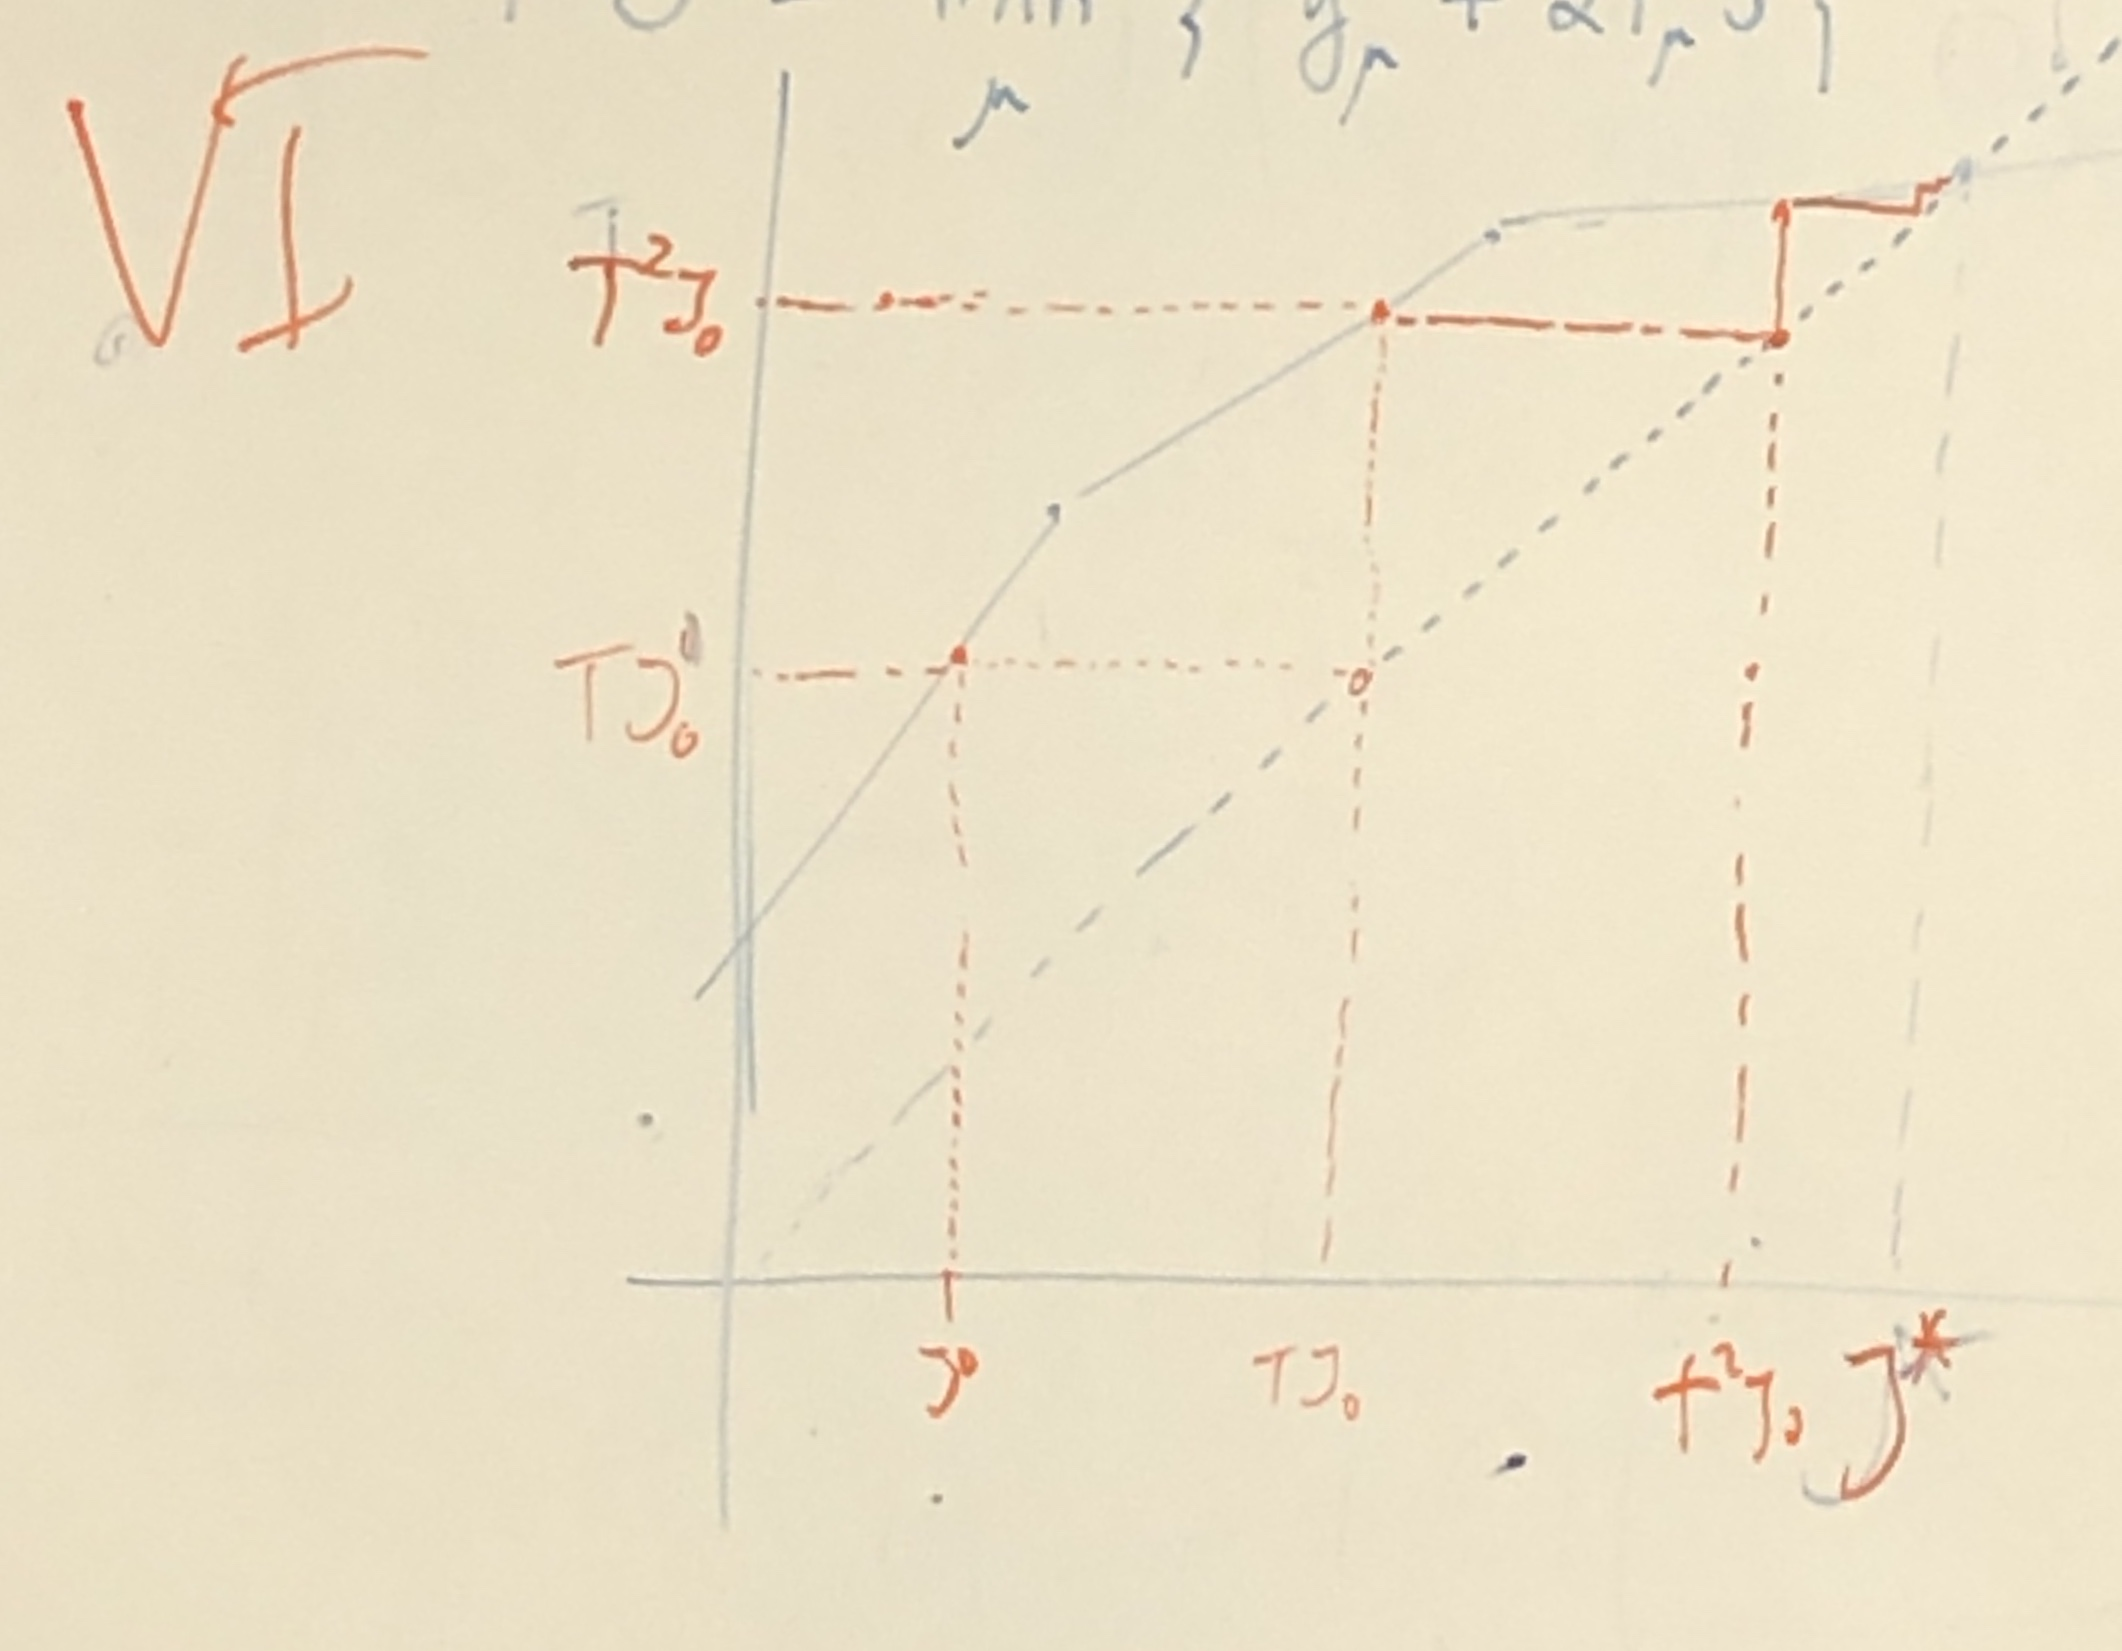
\includegraphics[scale=0.2]{stoch_dp_vi_vis}
\caption{Iteration of VI method. Start with \(J_0\), get \(T J_0\), plug in to \(T\), etc. Note that the optimal solution is the intersection of the \(TJ\) function and the 45 degree line, since the optimal policy satisfies \(TJ^* = J^*\).}
\label{stoch_dp_vi_vis_fig}
\end{center}
\end{figure}

Policy iteration is different. You fall into a policy, representing one piece of the function (one line segment---each one corresponds to a policy). Then compute \(J_{\mu^1}\), a fixed point of \(T_{\mu^1}\). \(T_{\mu^1}\) is the extension of the line segment corresponding to policy \(\mu^1\). So \(J_{\mu^1}\) is the point where that line intersects the 45 degree line \(T_{\mu^1} J = J\). Then you plug that point in and solve again, finding the next policy. Generally this approach is way faster (although in the worst case it can be very slow). See Figure \ref{stoch_dp_pi_vis_fig}. 

\begin{figure}[htbp]
\begin{center}
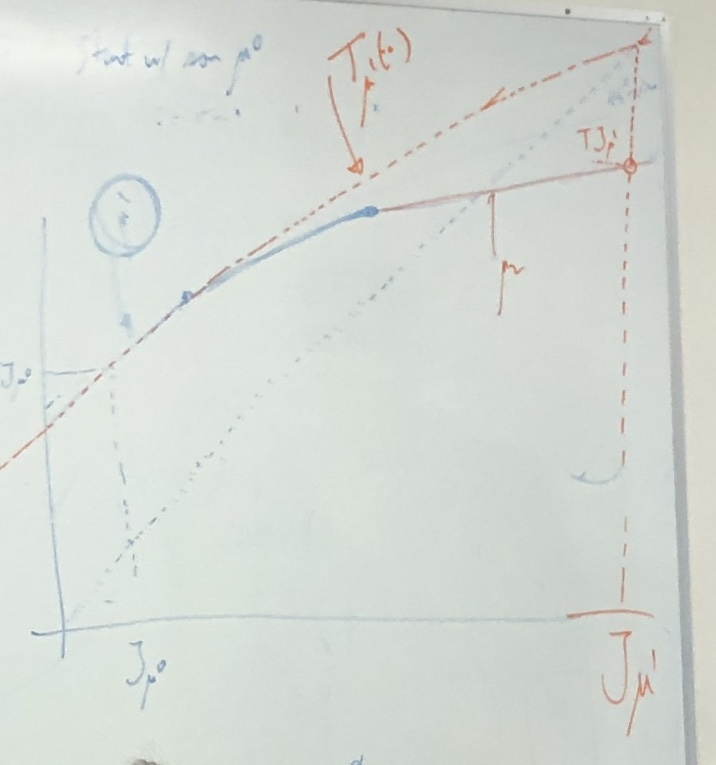
\includegraphics[scale=0.5]{stoch_dp_pi_vis}
\caption{Iteration of PI method.}
\label{stoch_dp_pi_vis_fig}
\end{center}
\end{figure}


\item \textbf{Optimistic policy iteration (blend of PI and VI; section 2.3.3 of \citet{v2_bertsekas2012dynamic})} Start with an initial \(J_0\). Let \(\{m_k: k = 0, 1, \ldots\}\) be any sequence of positive integers (say \(\{1, 1, 1, \ldots\}\). Do the following:

\begin{enumerate}

\item Take a greedy decision with respect to \(J_k\) to get the policy \(\mu^k\): \(T_{\mu^k} J_k = T J_k\). Then get \(J_{k+1} = T_{\mu^k}^{m_k} J_k\). If \(m_k = 1\) for all \(k\), we get value iteration: \(J_{k+1} = T_{\mu^k} J_k = T J_k\) for all \(k\). If \(m_k = \infty\) for all \(k\) (or is sufficiently large), we get \(J_{k+1} = J_{\mu^k}\), so \(T_{\mu^{k+1}} J_{k+1} = T J_{k+1}\). This is policy iteration. So this method subsumes PI and VI, and it doesn't require inverting a matrix like PI. Also we have lots of flexibility; converges to the optimal policy for any sequence (will prove next time).

\end{enumerate}

\begin{theorem}[\textbf{Proposition 2.3.2 of \citet{v2_bertsekas2012dynamic}}]

\(J_k\) coverges to \(J^*\) and \(\mu^k\) is optimal for all \(k\) sufficiently large.

\end{theorem}

\begin{proof}

``the same sequence of policies will be obtained" (p. 105): true because the costs differ only by constants, so the policy resulting in the optimum for both cost functions will be the same.

Prove by induction on \(k\) that \(\overline{J}_k \leq T \overline{J}_{k-1}\) and \(T \overline{J}_k \leq \overline{J}_k\). 

Base case: (\(k=1\)) we want to show that 

\[
\overline{J}_1 \leq T \overline{J}_0 , \qquad T \overline{J}_0 \leq \overline{J}_0.
\]

By definition, \(T_{\mu^0}\overline{J}_0 = T \overline{J}_0 \leq \overline{J}_0\) where the first step follows by definition of \(\mu^0\) and the second follows by our construction of \(\overline{J}_0\). So then \(T_{\mu^0}^m \overline{J}_0 \leq T_{\mu^0}^{m-1} \overline{J}_0 \) for all \(m\).

By definition (and using \(\overline{J}_1 = T_{\mu^0}^{m_0} \overline{J}_0\))

\[
T_{\mu_1} \overline{J}_1 = T \overline{J}_1 \leq T_{\mu^0} \overline{J}_1 = T_{\mu^0}^{m_0 + 1} \overline{J}_0 \leq T_{\mu^0}^{m_0} \overline{J}_0 = \overline{J}_1
\] 

where the second-to-last step follows from \(T_{\mu^0}^m \overline{J}_0 \leq T_{\mu_0}^{m-1} \overline{J}_0\) for all \(m\). But then \(\overline{J}_1 \leq T_{\mu^0}\overline{J}_0\), because to get \(\overline{J}_1\) we applied \(T_{\mu^0}\) \(m_0 \geq 1\) times. Therefore \(\overline{J}_1 \leq T \overline{J}_0\). 

Inductive step: Assume that \(\overline{J}_k \leq T \overline{J}_{k-1}\) and \(T \overline{J}_k \leq \overline{J}_k\). We want to show that \(\overline{J}_{k+1} \leq T \overline{J}_k\) and \(T \overline{J}_{k+1} \leq \overline{J}_{k+1}\).

By definition, \(T_{\mu^k} \overline{J}_k = T \overline{J}_k \leq \overline{J}_k\) where the last step follows by the inductive step. Therefore \(T_{\mu^k}^m \overline{J}_k \leq T_{\mu^k}^{m-1} \overline{J}_k\) for all \(m\) (same argument as above).

Finally, 

\begin{multline*}
T_{\mu^{k+1}} \overline{J}_{k+1} = T \overline{J}_{k+1} \leq T_{\mu^k}\overline{J}_{k+1} = \text{(by definition of \(\overline{J}_{k+1}\))} T_{\mu^k}^{m_k +1} \overline{J}_k \leq \text{(by above result) } T_{\mu^k}^{m_k} \overline{J}_k 
\\ = \overline{J}_{k+1} \leq T_{\mu^k}\overline{J}_k = T \overline{J}_k.
\end{multline*}

This gives us that \(\overline{J}_{k+1} \leq T \overline{J}_k\) and \(T \overline{J}_{k+1} \leq \overline{J}_{k+1}\). Now, note that 

\begin{align*}
& \overline{J}_1  \leq T \overline{J}_0
\\  \iff \qquad & \overline{J}_2 \leq T \overline{J}_1  \leq T^2 \overline{J}_0
\\  \iff \qquad & \overline{J}_3 \leq T \overline{J}_2   \leq T^2 \overline{J}_1 \leq T^3 \overline{J}_0
\end{align*}
which leads to \(\overline{J}_k \leq T^k \overline{J}_0\). Then to show \(J^* \leq \overline{J}_k\) for all \(k\), note that

\[
T \overline{J}_0 \leq \overline{J}_0 \implies J^* \leq \overline{J}_0
\]

because \(J^ = \lim_{k \to \infty} T^k \overline{J}_0 \). Also for all \(\ell\)

\[
T^\ell \overline{J}_k \leq T^{\ell-1} \overline{J}_k \leq \ldots \leq T \overline{J}_k \leq \overline{J}_k.
\]

\end{proof}

\begin{definition}[\textbf{One-step look-ahead policy; section 2.3.4, p. 106 of \citet{v2_bertsekas2012dynamic}}] If \(\tilde{J}\) is an approximation to \(J^*\), then a one-step look-ahead policy based on \(\tilde{J}\) is a policy \(\overline{\mu}\) such that \(T_{\overline{\mu}} \tilde{J} = T \tilde{J}\). 

\end{definition}

Note: can be an arbitrary vector \(\tilde{J}\). Also if \(\tilde{J} = J_\mu\) for some policy \(\mu\), then \(J_{\overline{\mu}}  \leq J_\mu\). Two-step lookahead:

\[
T_{\overline{\mu}} (T \tilde{J}) = T(T \tilde{J}).
\]



\begin{theorem}[\textbf{Proposition 2.3.3, p. 107 of \citet{v2_bertsekas2012dynamic}}]

Let \(\overline{\mu}\) be the one-step look-ahead policy based on \(\tilde{J}\), i.e., \(T_{\overline{\mu}} \tilde{J} = T \tilde{J}\). Let \(\hat{J} := T_{\overline{\mu}} \tilde{J} = T \tilde{J}\). Then

\begin{enumerate}[(a)]

\item If \(\hat{J} \leq \tilde{J}\), then \(J_{\overline{\mu}} \leq \hat{J}\).

\item  \(\lVert J_{\overline{\mu}} - \hat{J} \rVert \leq \frac{\alpha}{1-\alpha} \lVert \hat{J} - \tilde{J} \Vert\), \(J_{\overline{\mu}} - J^* \rVert \leq 2 \alpha/(1-\alpha)  \lVert \tilde{J} - J^* \rVert\), and \( \lVert J_{\overline{\mu}} - J^* \rVert \leq 2/(1-\alpha) \lVert \tilde{J} - \hat{J} \rVert\). 

\end{enumerate}

\end{theorem}

\begin{example}[\textbf{Example 2.3.1, p. 109 of \citet{v2_bertsekas2012dynamic}}]

Note that 

\[
T\tilde{J}(1) = \min\{0 + \alpha \tilde{J}(2), 2 \alpha \epsilon + \alpha \tilde{J}(1)\} = \min\{\alpha \epsilon, \alpha \epsilon\}  = \alpha \epsilon
\]

 and \(T\tilde{J}(2) = 0 + \alpha \tilde{J}(2) = \alpha \epsilon\).

So, with the one-step lookahead

\[
J_{\overline{\mu}}(1) = \frac{2 \alpha \epsilon}{1 - \alpha} =  \frac{2 \alpha}{1 - \alpha} \lVert \tilde{J} - J^* \rVert
\]

So

\[
\lVert J_{\overline{\mu}} - J^* \rVert = \frac{2 \alpha}{1 - \alpha} \lVert \tilde{J} - J^* \rVert
\]

so the bound is tight.

\end{example}

\begin{proposition}[\textbf{Proposition 2.3.4, p. 111 of \citet{v2_bertsekas2012dynamic}}]

\end{proposition}

\item \textbf{Linear programming (LP)}


Basic form: \(\max c^Tx \) s.t. \(Ax \leq b, x \geq 0\). Equivalent dual: \(\min \pi^Tb \) s.t. \(\pi^TA \geq c^T, \pi \geq 0\). Dual problem may have a smaller constraint set (number of variables in dual equals number of constraints in the primal). In primal problem: number of constraints equals number of state-action pairs, number of variables equals number of states. So both number of constraints and variables is large. So dual doesn't generally help a lot. But it turns out that for a variety of important problems there are ways to exploit the LP structure.

\end{enumerate}


exam: inventory, revenue management, VI (variants, applications in weird contexts), PI question for sure. so at least those 4 questions. maybe a 5th on one of these topics. optimistic PI maybe. LP no.



\subsection{Scheduling and Multiarmed Bandit Problems (Section 1.3 of  \citet{v2_bertsekas2012dynamic})}

We will examine the multiarmed bandit (MAB) in an infinite horizon discounted reward setting. (One of the few high-dimensional DPs that can be solved feasibly.) See setup on p. 22 of \citet{v2_bertsekas2012dynamic}. Other notation: \(x_k^\ell \in S^\ell\) (state space).

\[
J(x^1, \ldots, x^n) = \max_{u \in [n] }\left\{R^u(x^u) + \alpha \E[ J(x^1, \ldots, x^{u-1}, f^u(x^u, w^u), x^{u+1}, \ldots, x^n) \right\}
\]

(similar to equation (1.12) on p. 23, but without \(M\) retirement reward.)

Note this is high-dimensional: if each arm has 10 states, then the number of possible states is \(10^m\).

Key features: 

\begin{enumerate}

\item States of idle projects remain fixed.

\item Rewards received only depend on the state of selected arms.

\item Only one product can be chosen.

\end{enumerate}

Gittins in 1970s showed that an optimal policy for this problem is an index rule (equation (1.11) on p. 23). The index associated with each project can be computed by solving a 1 dimensional dynamic program. (i.e., solve \(n\) 1-dimensional problems rather than a single \(n\)-dimensional problem---much more feasible when \(n\) is large.)

First step to proving optimality of this approach: generalize the problem to allow the option of quitting at any time \(k\). Key: the retirement reward \(M\) will be crucial in defining our index function.

\begin{theorem}[\textbf{Proposition 1.3.4 in \citet{v2_bertsekas2012dynamic}, p. 29}]\label{statlearning.dp.prop.1.3.4.v2}

For each project \(\ell\), there exists a function \(m^\ell: S^\ell \to \mathbb{R}\) such that at each time \(k\) an optimal policy is given by the rule

\begin{itemize}

\item Retire if \(M > \max_{h \in [n]}\{m^{h}(x_k^{h})\}\),

\item Work on project \(\ell\) if \(m^\ell(x_k^\ell) = \max_{h \in [n]}\{m^{h}(x_k^{h}) \} \geq M\),

\end{itemize}

where the index function \(m^\ell(x^\ell)\) is as defined in (\ref{statlearning.dp.def.index.function}).

\end{theorem}

We will get some preliminary results to be able to prove this.

\begin{lemma}[\textbf{Proposition 1.3.1 in \citet{v2_bertsekas2012dynamic}, p. 29}]\label{statlearning.dp.prop.1.3.1.v2}

Let 

\[
B := \max_\ell \max_{x^\ell} | R^\ell(x^\ell)|.
\]

For fixed \(x \in S_1 \times \ldots \times S_n\), the optimal reward function (as a function of \(M\)) \(M \mapsto J(x,M)\) has the following properties:

\begin{enumerate}[(a)]

\item \(M \mapsto J(x,M)\) is convex and monotonically nondecreasing.

\item \(J(x, M)\) is constant for \(M \leq -B/(1-\alpha)\).

\item \(J(x,M) = M\) for all \(M \geq B/(1-\alpha)\).

\end{enumerate}

(See Figure \ref{dp_fig_1_3_1_fig}.)

\end{lemma}

\begin{figure}[htbp]
\begin{center}
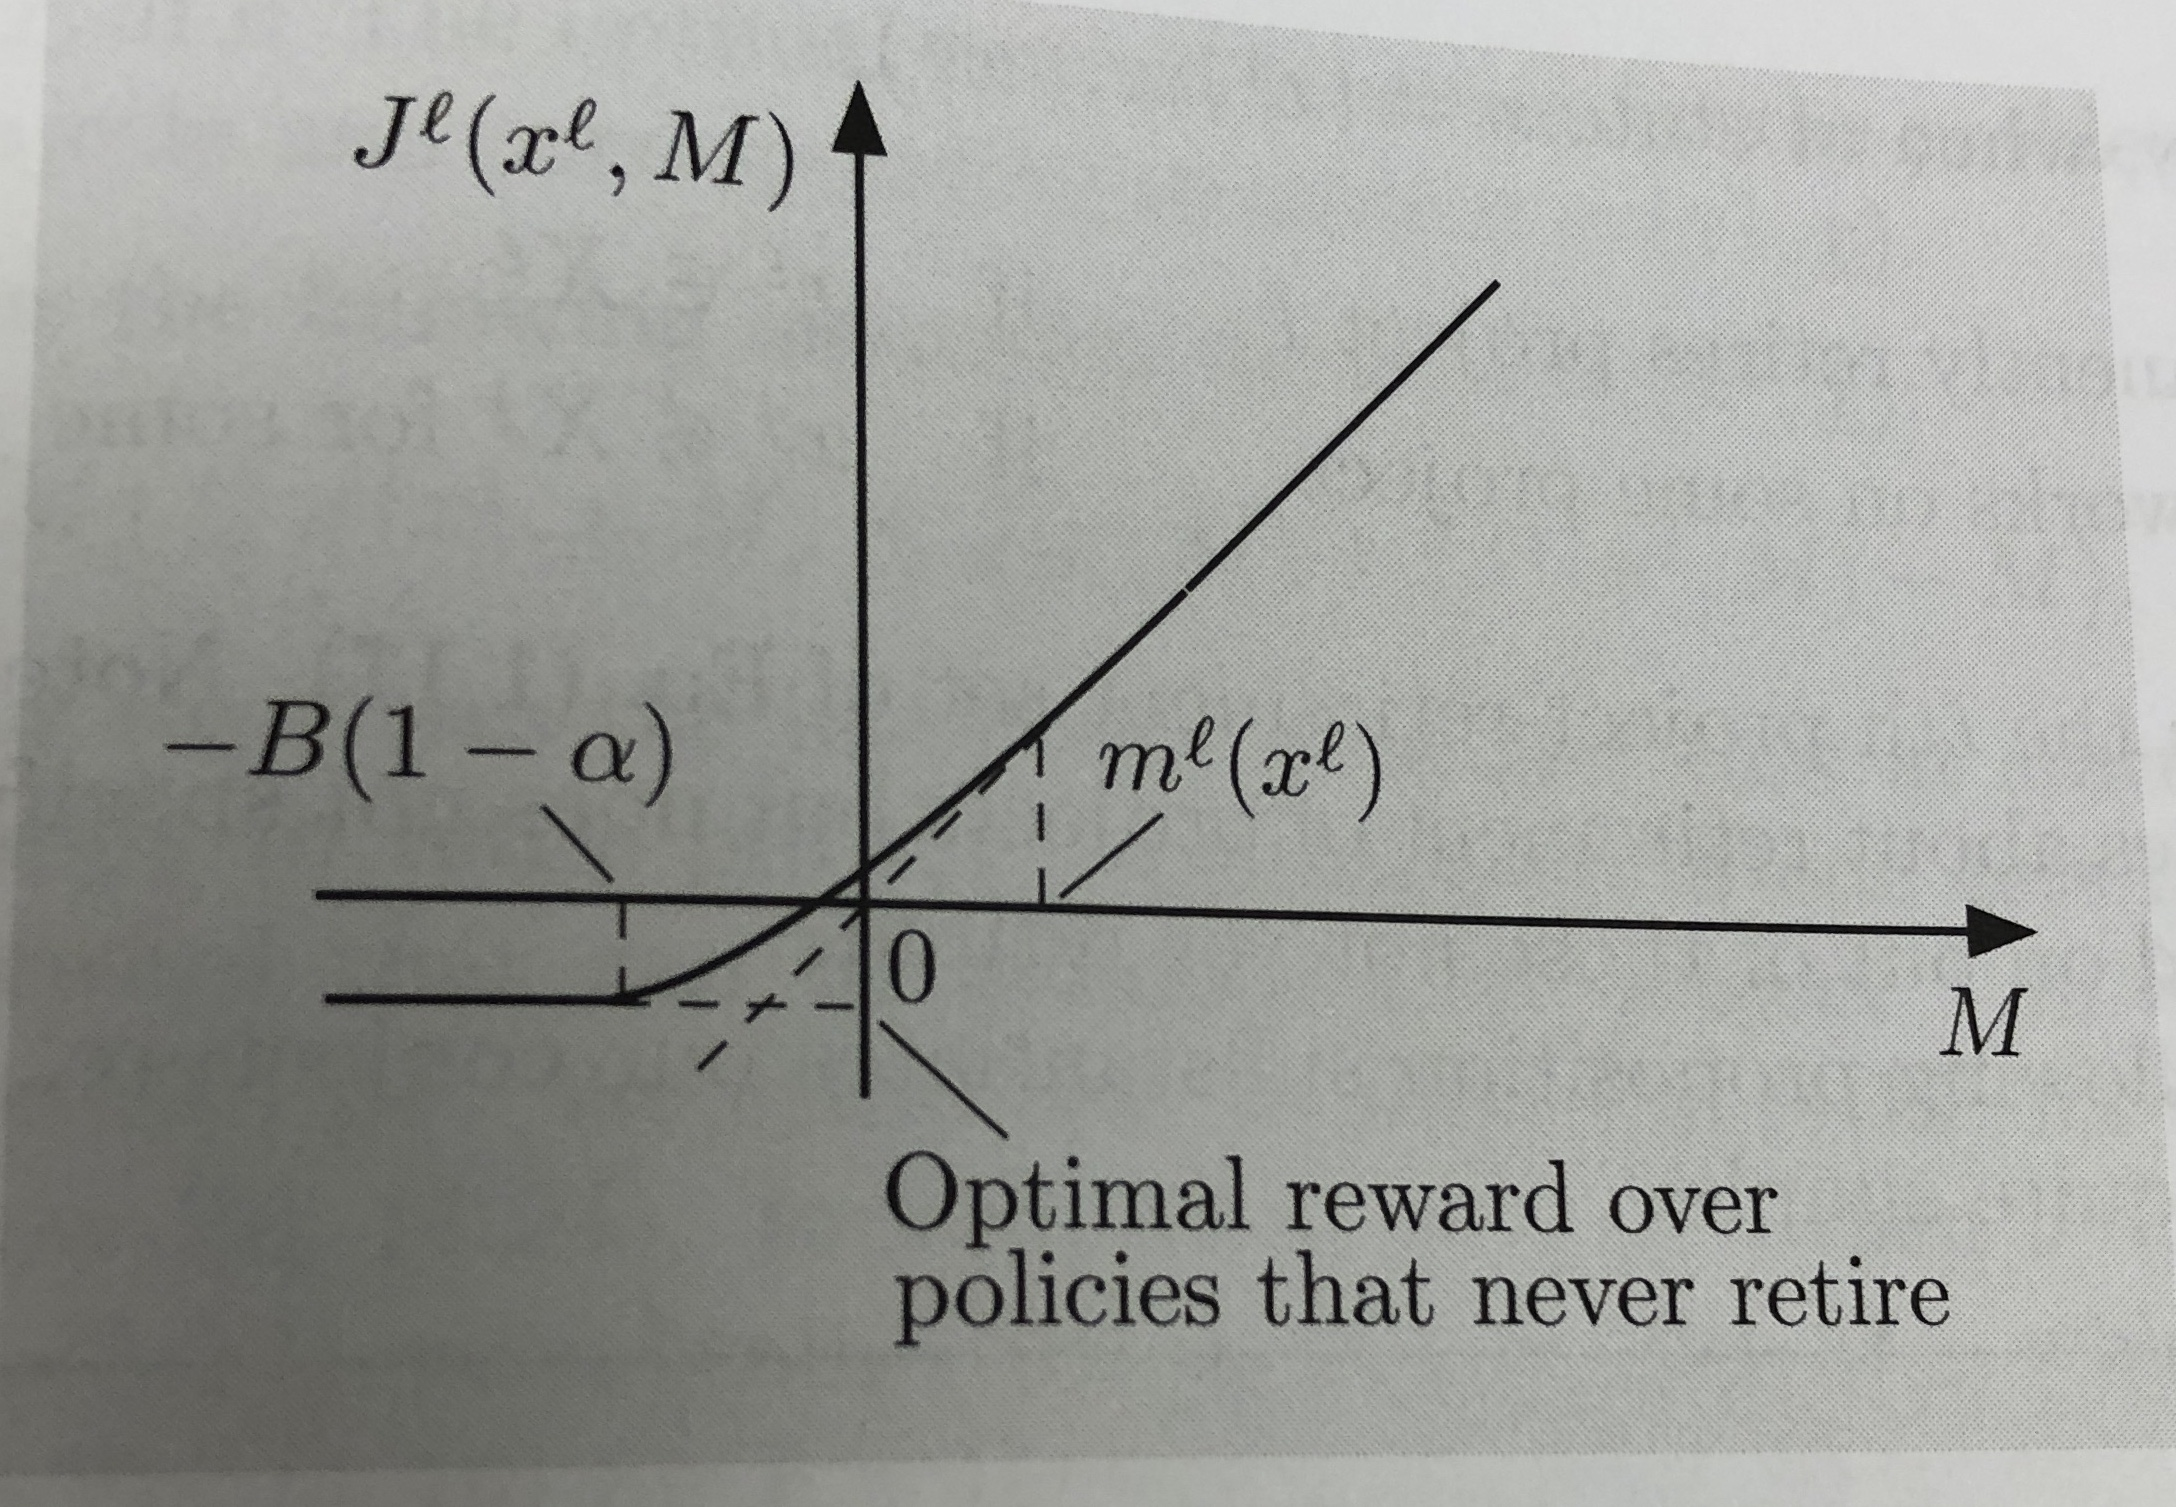
\includegraphics[scale=0.15]{dp_fig_1_3_1}
\caption{Figure 1.3.1 in \citet{v2_bertsekas2012dynamic}, p. 25. Form of the \(\ell\)th project reward function \(J^\ell(x^\ell, M)\) for fixed \(x^\ell\) and definition of the index \(m^\ell(x^\ell)\).}
\label{dp_fig_1_3_1_fig}
\end{center}
\end{figure}


\begin{proof}

\begin{enumerate}[(a)]

\item inductive step: recall that maximum of convex functions is convex. for each \(u\), get convex functions inside expectation. expectation preserves convexity, adding a constant preserves convexity, max preserves convexity. 

\item Note that the absolute worst reward you can ever get if you never retire is \(-B/(1-\alpha)\) (sum of infinite series if you get \(-B\) every time). So if \(M\) is worse than that, never makes sense to quit. 

\item Reverse of last argument.

\end{enumerate}

\end{proof}

Consider a situation with only one project (as on bottom of p. 24). There is a minimal value \(m^\ell(x^\ell)\) of \(M\) for which \(J^\ell(x^\ell, M) = M\) (the smallest \(M\) that would cause you to want to retire rather than work on your one project). That is,

\begin{equation}\label{statlearning.dp.def.index.function}
m^\ell(x^\ell) = \inf\{Q : Q =  J^\ell(x^\ell, Q)  \}.
\end{equation}

\begin{definition}[\textbf{Index function; p. 24 of \citet{v2_bertsekas2012dynamic}}]

The function \(m^\ell(x^\ell)\) as defined in (\ref{statlearning.dp.def.index.function}) is called the \textbf{index function} of project \(\ell\).

\end{definition}

The index function is the retirement reward for which we are indifferent between retiring and operating the project when at state \(x^\ell\). Note that \(m^\ell(x^\ell) \leq B/(1-\alpha)\), because per Lemma \ref{statlearning.dp.prop.1.3.1.v2}, we would always want to retire if \(M > B/(1-\alpha)\).

Total number of curves upper bounded by number of states times number of projects (as opposed to number of states raised to the number of projects---so big reduction). Also, each curve corresponds to a one-dimensional DP.

How do you find \(m^\ell(x^\ell)\) in practice? Easy to evaluate at a particular \(M\); solve the DP (value iteration, policy iteration, etc.). Use a bisection algorithm to find it (similar to finding a zero of a function). Have a bounded interval to start with: \([-B/(1-\alpha), B/(1- \alpha)]\). For each DP, number of state-action pairs is number of states times 2 (only 2 actions: retire or continue). 



\begin{definition}[\textbf{Project-by-Project Retirement Policy (PPR; pp. 25-26 of \citet{v2_bertsekas2012dynamic})}]

In a single project problem, the project is operated continuously up to the time that its state falls into the \textbf{retirement set}

\begin{equation}\label{statlearning.dp.retirement.set.def}
X^\ell = \{x^\ell : m^\ell(x^\ell) < M \}.
\end{equation}

A \textbf{project-by-project retirement policy} permanently retires projects in the same way as if they were the only project available:

\begin{itemize}

\item Permanently retire project \(\ell\) if \(x^\ell \in X^\ell\),

\item work on some project if \(x^j \notin X^j \) for some \(j\) (where \(X^j\) is the retirement set (\ref{statlearning.dp.retirement.set.def})). 

\end{itemize}

\end{definition}

Note that a PPR policy decides about retirement of projects but does not specify the project to be worked on out of those not yet retired.

\begin{proposition}[\textbf{Proposition 1.3.2 in \citet{v2_bertsekas2012dynamic}}]\label{statlearning.dp.prop.1.3.2.v2}

There exists an optimal PPR policy.

\end{proposition}

\begin{proof}

How to get (1.20):

\begin{align*}
m^\ell(x^\ell ) \geq M \qquad \implies  M & \leq R^\ell(x^\ell) + \alpha \E[J^\ell(f^\ell(x^\ell, w^\ell), M)] 
\\ & \leq R^\ell(x^\ell) + \alpha \E[J(x^1, \ldots, x^{\ell-1}, f(x^\ell, w^\ell), x^{\ell + 1}, \ldots, x^n, M)]
\\ & = L^\ell(x, M, J).
\end{align*}



\end{proof}

\begin{proposition}[\textbf{Proposition 1.3.3 in \citet{v2_bertsekas2012dynamic}}]\label{statlearning.dp.prop.1.3.3.v2}

For fixed \(x\), let \(K_M\) denote the (random) retirement time under an optimal policy when the retirement reward is \(M\). Then for all \(M\) for which \(\partial J (x, M)/ \partial M\) exists, we have

\[
\pderiv{J(x, M)}{M} = \E \left[ \alpha^{K_M} \mid x_0 = x \right].
\]

\end{proposition}

\begin{proof}

pp. 28- 29, \citep{v2_bertsekas2012dynamic}.

\end{proof}

Let \(T_\ell\) be the retirement time of project \(\ell\) if it were the only project available and let \(T\) be the retirement time for the multiproject problem. We have \(T = T_1 + T_2 + \ldots + T_n\) because the state of idle projects doesn't change. Further, all the \(T_\ell\) are independent. Therefore

\[
\E[\alpha^T] = \E[\alpha^{\sum_{\ell=1}^n T_\ell} ] = \prod_{\ell=1}^n \E[\alpha^{T_\ell}].
\]

Then Proposition \ref{statlearning.dp.prop.1.3.3.v2} yields

\begin{equation}
\pderiv{J(x, M)}{M} = \prod_{\ell=1}^n \pderiv{J^\ell(x^\ell, M)}{M}.
\end{equation}

We are now ready to prove Theorem \ref{statlearning.dp.prop.1.3.4.v2}.

\begin{proof}[Proof of Theorem \ref{statlearning.dp.prop.1.3.4.v2}]

notes for end of proof: The function \(M \mapsto J(x, M)\) and \(M \mapsto L^\ell(x, M, J)\) coincide at \(M = m(x)\). The derivatives of the two functions are the same for all \(M \leq m(x)\). Therefore for all \(M \leq m(x)\), \(J(x,M) = L^\ell(x, M, J)\), so it's optimal to choose project \(\ell\).

\end{proof}

\subsection{Approximate DP: Q-Learning (Section 6.3.3 of \citet{v1_bertsekas2012dynamic}, Sections 2.2.3, 2.5.3, and 6.1 - 6.6.1 of \citep{v2_bertsekas2012dynamic})}

We'll focus on large-scale DP under a discounted cost criterion. Interested in setting when the number of states is extremely large (say \(10^{100}\)).

How do we adapt VI for large-scale setting? \(VI: TJ \to J\).

\[
(TJ)(x) = \min_{u \in U(x)} \sum_{y \in S} P_{x,y}(u) [g(x,u,y) + \alpha J(y)].
\]

How do we compute the sum when the state space is so large? A potential approach is to use Monte Carlo simultion. We have that \(Y \sim P_{x, \cdot}(u)\), and the sum is \(\E[g(x, u,Y) + \alpha J(Y)]\). Suppose we want to compute \(\E[F(Z)]\) for some function \(F\). The true value is \(\sum_{z \in S} \mathbb{P}(z) F(z)\), but if \(|S|\) is intractably large, consider an IID sample \(z_1, \ldots, z_K \) drawn from \(Z\). The Strong Law of Large Numbers tells us \(\frac{1}{k} \sum_{k=1}^K F(z_k) \xrightarrow{a.s.} \E[F(Z)]\). If \(K \ll |S|\), this sample is much easier to compute.

How large should the number of samples be? Recall Chebyshev's Inequality (\ref{asym.cheby}):

\[
\mathbb{P}\left(  \left|  \frac{1}{K} \sum_{k=1}^K F(z_k) - \E[F(Z)] > \right| \epsilon \right) \leq \delta
\]

if \(K \geq \frac{1}{\delta} \frac{\Var(F(Z))}{\epsilon^2}\).

We will combine Monte Carlo simulation with VI. To avoid the sum, for each \(u \in U(x)\), we can sample \(y_1, \ldots, y_K\) according to \(P_{x, \cdot}(u)\) and approximate

\[
\sum_{y \in S} P_{x,y}(u) [g(x,u,y) + \alpha J(y)] \approx  \frac{1}{K} \sum_{k=1}^K \left[ g(x,u,y_k) + \alpha J(y_k) \right] .
\]

Do we do this for each \(u \in U(x)\)? (Do we generate a new sample for each \(u \in U(x)\)?) What about for each \(x\)---do I have to update all states simultaneously? Can I update one state at a time?

\begin{definition}

Let 

\[
Q_k(x_k, u_k) :=  \E \left[g_k(x_k, u_k, y_k) + J_{k+1}(f_k(x_k, u_k, y_k)) \right] =  \sum_{y \in S} P_{x,y}(u) \left[ g_k(x_k, u_k, y_k) + \alpha J^*(y) \right].
\]

Let the optimal \(Q^*\) be defined by

\[
Q^*(x,u) := \sum_{y \in S} P_{x,y}(u) \left[ g(x, u, y) + \alpha J^*(y) \right], \qquad J^*(x) = \min_{u \in U(x)} Q^*(x,u).
\]

(Note that this is simply a re-writing of Bellman's Equation. See Section 6.3.3 of \citet{v1_bertsekas2012dynamic}, p.339 - 340.)

\end{definition}

Suppose we're given \(Q_k(\cdot, \cdot)\) based on sample \(y_1, y_2, \ldots, y_{k-1}\). Then

\[
Q_{k+1}(x,u) = \frac{1}{k} \sum_{\ell=1}^k [g(x, u, y_\ell) + \alpha \min_{v \in U(y_\ell)} Q_\ell(y_\ell, v)].
\]

Note: for each iteration, we only have one new sample.

\[
Q_{k+1}(x,u) = \frac{1}{k}\left[ g(x, u, y_k)  + \alpha \min_{v \in U(y_\ell)} Q_k(y_\ell, v) \right ] + \frac{k-1}{k} \cdot  \underbrace{\frac{1}{k-1}  \sum_{\ell=1}^{k-1} [g(x, u, y_\ell) +  \min_{v \in U(y_\ell)} Q_\ell(y_\ell, v)]}_{Q_k(x, u)}.
\]

Therefore 

\begin{align*}
Q_{k+1}(x,u) & = \frac{1}{k}\left[ g(x, u, y_k)  + \alpha \min_{v \in U(y_\ell)} Q_k(y_\ell, v) \right] + \underbrace{\frac{k-1}{k}}_{= 1 - 1/k} Q_k(x, u)
\\ & = Q_k(x,u) + \frac{1}{k} \left[g(x, u, y_k) + \alpha \min_{v \in U(y_\ell)} Q_k(y_\ell, v) - Q_k(x,u) \right] .
\end{align*}

Q-learning (algorithm from section 6.6.1 of \citet{v2_bertsekas2012dynamic}, p. 496):

\[
Q_{k+1}(x, u) = Q_k(x, u) + \gamma_k  \left[g(x, u, y_k) + \alpha \min_{v \in U(y_\ell)} Q_k(y_\ell, v) - Q_k(x,u) \right] .
\]

where \(\gamma_k\) is the step size.

\begin{theorem}[\textbf{Section 6.6.1 of \citet{v2_bertsekas2012dynamic}, p. 496}]
If each \(Q(x,u)\) is updated infinitely often and \(\sum_{k=1}^\infty \gamma_k = \infty\), \(\sum_{k=1}^\infty \gamma_k^2 < \infty\), then \(Q_k \to Q^*\).

\end{theorem} 

(See Section 6.3 of \citet{v2_bertsekas2012dynamic} for this material.) How do we deal with a huge number of states? Our goal is to compute \(\{J^*(x): x \in S\}\), but \(|S|\) is huge. Approximate \(J^*(x) \approx \sum_{k=1}^K \phi_k(x) \cdot r_k = (\Phi r)(x) \), where \(\Phi \in \mathbb{R}^{|S| \times K}\) and \(r \in \mathbb{R}^K\). Important: we do not store \(\Phi\) explicitly. We compute \(\phi_k(x)\) as needed.

Our goal is to find \(r\) such that \(\Phi r\) is close to \(J^*\). We do this by projecting \(J^*\) onto the span of \(\Phi\); that is, we would like to compute

\begin{equation}\label{statlearning.qlearning.opt}
\min_{r \in \mathbb{R}^K} \sum_{x \in S} \pi(x) \left( (\Phi r)(x) - J^*(x) \right)^2.
\end{equation}

More compact notation:

\[
\lVert \Phi r - J^* \rVert_\pi^2 := (\Phi r - J^*)^T D ( \Phi r - J^*)
\]

where

\[
D = \begin{pmatrix}
\pi(1) & \ldots & 0 \\
\vdots & \ddots & \vdots \\
0 & \ldots & \pi(S)
\end{pmatrix}.
\]

\textbf{and \(\lVert \cdot \rVert_\pi\) is a weighted norm under the stationary probability distribution \(\pi\) of the transition matrix \(P\). For any vector \(J\)}

\[
\lVert J \rVert_\pi = \sqrt{\sum_{x \in S} \pi(x) | J(x)|^2 }.
\]

 Then we can write (\ref{statlearning.qlearning.opt}) as

\[
\min_{r \in \mathbb{R}^K} \lVert \Phi r - J^* \rVert_\pi^2
\]

Instead of summing over all states, we sample the states according to \(\pi(\cdot)\), so \(x_1, x_2, \ldots, x_n\). Then we find

\[
\min_{\pi \in \mathbb{R}^K} \frac{1}{n} \sum_{i =1}^n \left( (\Phi r)(x_i) - J^*(x_i)  \right)^2.
\]

However, this problem is still not tractable because we do not know \(J^*\). Idea: leverage the ``closed form" expression for the optimal \(r^*\) (if we have \(J^*\))

\begin{align*}
0  & = \nabla_r \lVert J^* - \Phi r \rVert_\pi^2 
\\ & = \nabla_r \left[ (\Phi r - J^*)^T D ( \Phi r - J^*) \right] 
\\ & = 2 \Phi^TD(\Phi r - J^*)
\\ \implies \qquad r^* & = (\Phi^T D \Phi)^{-1} \Phi^T D J^*, 
\\ \Phi r^* & = \Phi  (\Phi^T D \Phi)^{-1} \Phi^T D J^*.
\end{align*}

Observe that \(\Phi  (\Phi^T D \Phi)^{-1} \Phi^T D \) is a projection matrix \(\Pi\).

where \(\Pi\) is the projection onto the basis functions \(\phi\); projection with respect to \(\lVert \cdot \rVert_\pi\), and \(\pi\) is the stationary distribution of the transition matrix \(P\) \textbf{(key: only one transition matrix, as in optimal stopping; see below)}.



Intuition: start with an initial \(J\). Do approximate value iteration:

\[
\Pi T J \in \mathbb{R}^{|S|}
\]

project \(TJ\) into the \(K\)-dimensional vector space spanned by \(\phi_1, \ldots, \phi_K\). Don't keep track of the full \(TJ\); instead, just the \(K\) coefficients. 

%\[
%Q_{k+1}(x,u) = \frac{1}{k} \left[ g(x, u, y_k) + \alpha \min_{v \in U(y_k)} Q_k(y_k, v) 
%\]

Approximate VI: \((\Pi T)^k J \). Caveat: this update can lead to (??).

\begin{example}[Example 6.4.2 in \citet{v2_bertsekas2012dynamic}, p. 472]

\end{example}

Proposed method: start at \(r^{(0)} \in \mathbb{R}^K\). Iteration:

\begin{align*}
r^{(k+1)} & = \underset{r \in \mathbb{R}^K}{\arg \min} \lVert \Phi r - T \Phi r^{(k)} \rVert_\pi^2
\\ \iff \qquad \Phi r^{(*k+1)} & = \Pi T(\Pi r(^{(k)}),
\end{align*}

where \(\Pi = \Phi(\Phi^T D \Phi)^{-1} \Phi^T D\), with \(D\) as defined before.

\begin{lemma}[\textbf{Lemma 6.3.1 in \citet{v2_bertsekas2012dynamic}, p. 427}]

If \(\Pi'P = \Pi'\), then \(\lVert PJ \rVert_\Pi \leq \lVert J \rVert_\Pi\).

\end{lemma}

\begin{proof}

\begin{align*}
\lVert PJ \rVert_\Pi^2 = \sum_{x \in S} \pi(x) \left[ (PJ)(x) \right]^2 = \sum_{x \in S} \pi(x) \left( \sum_{y \in S} P_{x,y} J(y) \right)^2 \leq \text{ (by Jensen's inequality) } \sum_{x \in S} \pi(x) \sum_{y \in S} P_{x,y}(J(y))^2 = \sum_{y \in S}[J(y)]^2 \underbrace{ \sum_{x \in S} \pi(x) P_{x,y} }_{\Pi(y)} = \sum_{y} \pi(y)[J(y)]^2 = \lVert J \rVert_\pi^2.
\end{align*}

\end{proof}

\begin{lemma}[\textbf{Proposition 6.3.1(a) in \citet{v2_bertsekas2012dynamic}, p. 429}]

Consider a policy \(\mu\). Let \(P\) be the transition matrix associated with \(\mu\). If \(\Pi' P = \Pi'\) then \(\lVert T_\mu J - T_\mu \overline{J} \rVert_\Pi \leq \alpha \lVert J - \overline{J} \rVert_\Pi\).

\end{lemma}

\begin{proof}

\[
\lVert T_\mu J - T_\mu \overline{J} \rVert_\Pi^2 = \sum_{x \in S} \pi(x) \left[(T_\mu J)(x) - (T_\mu \overline{J})(x) \right]^2 = \sum_{x \in S} \pi(x) \left[ \alpha \sum_y P_{x,y} \left( J(y) - \overline{J}(y) \right) \right]^2 = \alpha^2 \sum_{x \in S} \pi(x) \left[ (P(J - \overline{J}))(x) \right]^2 = \alpha^2 \lVert P(J - \overline{J}) \rVert_\pi^2 \leq \text{ (by previous Lemma) } \alpha^2 \lVert J - \overline{J} \rVert_\pi^2
\]

because 

\[
(T_\mu J)(x) = g(x, \mu(x)) + \alpha \sum_y P_{x, y} ( \mu(x)) J(y).
\]

\end{proof}

\(\Pi\) is expansive under the sup norm. However...

\begin{lemma}[\textbf{Proposition 6.3.1(a) in \citet{v2_bertsekas2012dynamic}, p. 429}]

The projection matrix \(\Pi\) is nonexpansive with respect to \(\lVert \cdot \rVert_\Pi\); i.e., \(\Pi J \rVert_\Pi \leq \lVert J \rVert_\Pi\).

\end{lemma}

\begin{proof}

We begin by observing that \(J - \Pi J\) is orthogonal to \(\Pi J\). 

\[
\Pi(J - \Pi J) = \Pi J - \Pi \Pi J = 0.
\]

So \(J - \Pi J\) is in the nullspace of \(\Phi r\). Then

\[
\lVert J \rVert_\pi = \lVert J - \Pi J \rVert_\pi + \lVert \Pi J \rVert_\pi \geq \lVert \Pi J \rVert_\pi.
\]

\end{proof}

We know have that \(\Pi T_\mu\) is a contraction mapping with respect to \(\lVert \cdot \rVert_\pi\), where \(\pi\) is the stationary distribution with respect to \(P_\mu\). \textbf{This result ends up showing that \(Q_{k+1} \to \hat{Q}\) because \(\Pi \circ F\) is a contraction mapping under \(\lVert \cdot \rVert_\pi\) and \(\hat{Q}\) is the unique fixed point of \(\Pi \circ F\); that is, \(\Pi F \hat{Q} = \hat{Q}\).} How do we compute \((\Pi T)J\) with \(J = \Phi r^{(k)}\)?

\begin{enumerate}

\item Sample \(x_1, \ldots, x_n\) from \(\pi\).

\item Solve 

\[
r^{(k+1)} := \underset{r \in \mathbb{R}^K}{\arg \min} \frac{1}{n} \sum_{i=1}^n \left[ (\Phi r)(x_i) - (\Phi r^{(k)})(x_i) \right]^2
\]

\end{enumerate}

How do you get \(\pi\)? Simulate using a Markov chain for as long as needed; eventually converges to stationary distribution. 

Note: divergence can occur if the wrong norm is used. We have convergence if 

\begin{enumerate}

\item 

\[
(TJ)(x) = \sum_{y \in S} P_{x,y} (g(x,y) + \alpha J(y)) 
\]

(only one action)

\item \( \pi^T P = \pi^T.\)

\end{enumerate}

Heuristic for Approximate VI for general MDP. Initialization: given \(\Phi = \begin{bmatrix} \phi_1 & \cdots & \phi_k \end{bmatrix}\) and \(r^{(0)}\).

\begin{enumerate}

\item Given \(r^{(k)}\), sample \(x_1, \ldots, x_n\) from a distribution \(\pi\). Then

\[
r^{(k+1)} := \underset{r \in \mathbb{R}^K}{\arg \min} \frac{1}{n} \sum_{i=1}^n \left[ ( \Phi r)(x_i) - (T \Phi r^{(k)})(x_i) \right]^2.
\]

\[
(T \Phi r)(x) = \min_{u \in U(x)} \sum_{y \in S} P_{x,y}(u) \left[ g(x, u, y) + \alpha( \Phi r)(y) \right]^2
\]

\item

\end{enumerate}

(can't prove anything about this, just a ``hack," but seems to work.)

\subsection{Optimal Stopping (Section 6.6.4 of \citet{v2_bertsekas2012dynamic}, p. 504)}

Key insight: in an optimal stopping problem, there is one transition matrix.

Want a high-dimensional MC. (\(X_t \in S: t= 1, 2, \ldots\))

DP operator:

\[
(TJ)(x) = \max\{g(x), h(x) + \alpha \sum_{y \in S} P_{xy} J(y) \} = h(x) + \max\{ g(x) - h(x), \alpha \sum_{y \in S} P_{x,y} J(y) \}.
\]

\[
TJ = \max\{g, \alpha PJ \}.
\]

Still suffer from curse of dimensionality even though we only have one DP.

\[
Q^*(x) := \alpha \sum_{y \in S} \phi_{x, y} J^*(y) = \underbrace{\alpha \sum_{y \in S} P_{x,y} \max\{g(y), Q^*(y)\}}_{(FQ^*)(x)}, \qquad J^*(x) = \max\{ \underbrace{g(x)}_{\text{reward for stopping}} , \underbrace{Q^*(x)}_{\text{reward for continuing}}\}.
\]

\(Q^*\) is the optimal value you get if you continue---the \textbf{optimal continuation function.} 

\[
Q^* = \alpha P J^* = \alpha P \max\{g, Q\} \qquad \iff \qquad Q^* = F Q^*
\]

where \(FQ = \alpha P \max\{g, Q\}\). So \(Q^*\) is the fixed point of a contraction mapping.

We'll approximate \(Q^*\) in general as a sequence of coefficients \(r^{(1)}, r^{(2)}, \ldots\). Given \(r^{(k)}\), 

\begin{enumerate}

\item Sample \(x_{k+1} \sim \pi\), where \(\pi\) is the stationary distribution of \(P\). \(y_{k+1} \sim P_{x_{k+1}}\). 

\item 

\[
r^{(k+1)} := \underset{r \in \mathbb{R}^K}{\arg \min} \left\{  \frac{1}{k+1} \sum_{\ell=1} \left[^{k+1} (\Phi r)(x_i) - \alpha \max \{g(y_\ell), (\Phi r^{(k)} )(y_\ell) \right]^2 \right\}
\]

(so we are using \( (\Phi r^{(k)} )(y_\ell)\) as an approximation for \(Q^*(y)\)).

\end{enumerate}

As \(k \to \infty\), \(\lVert \Phi r - F \Phi r^{(k)} \rVert_\pi^2\). Again,

\[
(FQ)(x) = \alpha \sum_{y \in S} P_{x,y} \max\{g(y), Q(y) \}.
\]

With one sample we can get an unbiased estimate of \((FQ^*)(x)\). Does the iterate \(Q := \Pi F Q\) converge? Yes.

\begin{lemma}[\textbf{Proposition 6.6.1 in \citet{v2_bertsekas2012dynamic}, p. 506}]

\(F\) is a contraction mapping with respect to \(\lVert \cdot \rVert_\pi\).

\end{lemma}


\begin{proof}
p. 506 of \citet{v2_bertsekas2012dynamic}.
\end{proof}

Question: given \(k\), \((\Pi F)^kQ \to \tilde{Q}\), how close is \(\tilde{Q}\) to \(Q^*\)? Note \(\tilde{Q} \neq \Pi Q^*\). Rather, \(\tilde{Q}\) is the fixed point of \(\Pi F\); \(\tilde{Q} = \Pi F \tilde{Q}\). 

\begin{theorem}

\[
\lVert \tilde{Q} - Q^* \rVert_\pi \leq \frac{1}{\sqrt{1 - \alpha ^2}} \lVert \Pi Q^* - Q^* \rVert_\pi.
\]

\end{theorem}

\begin{proof}

Observe that \(\tilde{Q} \in \operatorname{span} \Phi\). Also, \( \Pi \tilde{Q} \in \operatorname{span} \Phi\). Therefore \(\tilde{Q} - \Phi Q^* \perp \Pi Q^* - Q^*\) since \(\Pi Q^* - Q^*\) is in the nullspace of \(\Phi\). Now

\begin{align*}
\lVert \tilde{Q} - Q^* \rVert_\pi^2 & = \lVert \tilde{Q} - \Pi Q^* _ \Pi Q^* - Q^* \rVert_\pi^2 
\\ & = \lVert \tilde{Q} - \Pi Q^* \rVert_\pi^2 + \lVert \Pi Q^* - Q^* \rVert_\pi^2
\\ & = \Pi F \tilde{Q} - \Pi F Q^* \rVert_\pi^2 + \lVert \Pi Q^* - Q^* \rVert_\pi^2
\\ \leq \alpha \lVert \tilde{Q} - Q^* \rVert_\pi^2 + \lVert \Pi Q^* - Q^* \rVert_\pi^2 
\end{align*}

because \(\Pi Q^* = \Pi FQ^*\) and \(\Pi F\) is a contraction mapping. Observe that

\[
\lVert \tilde{Q} - Q^* \rVert_\pi \leq \frac{\lVert \Pi Q^* - Q^* \rVert_\pi^2}{\sqrt{1 - \alpha^2}}.
\]

\end{proof}

\textbf{proved error bound: \(\lVert \hat{Q} - Q^* \rVert_\pi \leq \frac{1}{\sqrt{1 - \alpha^2}} \cdot \lVert \Pi Q^* - Q^* \rVert_\pi\). This error bound highlights the importance of choosing a good approximation architecture. \(\Phi\) has a span of \(K\) basis vectors; if it is close to \(Q^*\), so is the projection of \(Q^*\) onto the span of \(\Phi\).}

Question: how well does a policy generated from \(\hat{Q}\) perform? An approach: let \(\hat{J} := \max\{g, \hat{Q}\}\) and \(\hat{J}\) will be our approximation of \(J^*\) (the optimal value function). Let \(\mu\) be a greedy policy with respect to \(\hat{J}\); that is, \(T_\mu \hat{J} = T \hat{J}\). From our lecture in Week 6,

\begin{align*}
\lVert J^* - J_\mu \rVert_\infty & \leq \frac{2 \alpha}{1-\alpha} 
\\ & \leq \frac{2\alpha}{1-\alpha} \lVert Q^* - \hat{Q} \rVert_\infty,
\end{align*}

but this distance can diverge to \(\infty\) under \(\lVert \cdot \rVert_\infty\). So we need a slightly different approach.

A new approach: \(\hat{Q}\) is our approximation of \(Q^*\), which is the optimal value of continuing on. Let \(\hat{\tau}\) be a random variable for the stopping time derived from \(\hat{Q}\); that is,

\[
\hat{\tau} = \min\{t: \hat{Q}(x_t) \leq g(x_t)\}.
\]

\(x_t\) is well-defined because we have one transition matrix (one Markov chain). This defines a policy (as long as approximate value of continuing is greater than stopping, keep going; once reversed, stop.) That is, the stopping region derived from \(\hat{Q}\) is given by

\[
\{x: \hat{Q}(x) \leq g(x)\}.
\]

Recall again that \(x\) may in general be extremely high-dimensional. Note: the optimal stopping region is 

\[
\{x: Q^*(x) \leq g(x)\}.
\]

The payoff associated with the policy derived from \(\hat{Q}\) is given by

\[
J_{\hat{\tau}}(x) = \E \left[ \alpha^{\hat{\tau}} g(x_{\hat{\tau}}) \mid X_0 = x \right]
\]

Let 

\[
\tau^* = \min\{t: Q^*(x_t) \leq g(x_t)\}.
\]

 denote the (actual) optimal stopping time. The optimal expected reward is
 
 \[
 J^*(x) = \E \left[ \alpha^{\tau^*} g(x_{\tau^*}) \mid X_0 = x \right].
 \]
 
 Our goal is to compare \(J^*\) with \(J_{\hat{\tau}}\). 
 
 \begin{theorem}
 
 \[
 \lVert J^* - J_{\hat{\tau}} \rVert_\pi \leq \frac{1}{1-\alpha} \lVert \hat{Q} - Q^* \rVert_\pi.
 \]
 
 \end{theorem}
 
 \begin{remark}
 
 \textbf{Observe that combining this result with the result from last time yields}
 
  \begin{align*}
 \lVert J^* - J_{\hat{\tau}} \rVert_\pi  & \leq \frac{1}{1-\alpha} \lVert \hat{Q} - Q^* \rVert_\pi
 \\ & \leq \frac{1}{(1-\alpha)\sqrt{1- \alpha^2}} \lVert \Pi Q^* - Q^* \rVert_\pi.
 \end{align*}
 
 \end{remark}
 
 \begin{proof}
 
 Let \(Q_{\hat{\tau}}(x)\) be the expected reward of the following policy: continue the process in the next step and follow the policy based on \(\hat{\tau}\) thereafter. 
 
 We claim that \(\lVert J^* - J_{\hat{\tau}} \rVert_\pi \leq \lVert Q^* - \hat{Q} \rVert_\pi +  \lVert Q^* -  Q_{\hat{\tau}} \rVert_\pi \). (Note that \(Q_{\hat{\tau}} \neq \hat{Q}\). \(\hat{Q}\) is derived from approximate value iteration; it is the unique fixed point of \(\Pi F(\cdot)\). \(Q_{\hat{\tau}}\) is the value of a policy.)
 
 To prove this claim, note that 
 
 \begin{align*}
 J^*(x) - J_{\hat{\tau}}(x)  & = \begin{cases}
 \max\{g(x), Q^*(x)\} - g(x) , & g(x) \geq \hat{Q}(x),
 \\   \max\{g(x), Q^*(x)\} - Q_{\hat{\tau}}(x) , & g(x) < \hat{Q}(x).
 \end{cases}
 \\ & = \begin{cases}
g(x) - g(x) = 0 , & g(x) \geq \hat{Q}(x), g(x) \geq Q^*(x)
 \\  Q^*(x) - g(x) , & g(x) \geq \hat{Q}(x), g(x) < Q^*(x)
  \\   Q^*(x) - Q_{\hat{\tau}}(x) , & g(x) < \hat{Q}(x), g(x) < Q^*(x),
   \\   g(x) - Q_{\hat{\tau}}(x) , & g(x) < \hat{Q}(x), g(x) \geq Q^*(x).
 \end{cases}
 \end{align*}
 
 Consider the cases one at at time.
 
 \begin{enumerate}
 
 \item \(J^*(x) - J_{\hat{\tau}}(x) = g(x) - g(x) = 0\).
 
 \item Since \(J^*\) is optimal, \(0 \leq J^*(x) - J_{\hat{\tau}}(x) = Q^*(x) - g(x) \leq Q^*(x) -  \hat{Q}(x)\) since by assumption of this case \(\hat{Q}(x) \leq g(x)\). 
 
 \item We already have what we need: \(0 \leq J^*(x) - J_{\hat{\tau}}(x) = Q^*(x) - Q_{\hat{\tau}}(x)\). 
 
 \item We have \(Q^*(x) \leq g(x) < \hat{Q}(x)\) by assumption. Then 
 
 \begin{align*}
 0 & \leq J^*(x) - J_{\hat{\tau}}(x) 
 \\ & = g(x) - Q_{\hat{\tau}}(x) 
 \\ & \leq \hat{Q}(x) - Q_{\hat{\tau}}(x)
 \\& = \underbrace{\hat{Q}(x) - Q^*(x)}_{\geq 0 \text{ by assumption}}  + \underbrace{Q^*(x) - Q_{\hat{\tau}}(x)}_{\geq 0 \text{ because \(Q^*\) is optimal}}
 \end{align*}
 
 \end{enumerate}
 
 In all four cases, \(\lVert J^* - J_{\hat{\tau}} \rVert_\pi \leq \lVert Q^* - \hat{Q} \rVert_\pi +  \lVert Q^* -  Q_{\hat{\tau}} \rVert_\pi \), proving the claim. 
 
 Now we want to use the claim to prove the theorem. We have
 
 \begin{align*}
 \lVert J^* - J_{\hat{\tau}} \rVert_\pi & \leq \lVert Q^* - \hat{Q} \rVert_\pi +  \lVert Q^* -  Q_{\hat{\tau}} \rVert_\pi
 \\ & =  \lVert Q^* - \hat{Q} \rVert_\pi +  \lVert \alpha P J^* - \alpha PJ_{\hat{\tau}}  \rVert_\pi
 \\ & \leq \lVert Q^* - \hat{Q} \rVert_\pi +   \alpha  \lVert  J^* - J_{\hat{\tau}}  \rVert_\pi
 \end{align*}
 
 where the second inequality followed because \(P\) is a nonexpansive mapping. Therefore
 
 \begin{align*}
  \lVert J^* - J_{\hat{\tau}} \rVert_\pi & \leq \frac{1}{1-\alpha}  \lVert Q^* - \hat{Q} \rVert_\pi 
  \\ & \leq \frac{1}{1-\alpha} \cdot \frac{1}{\sqrt{1-\alpha^2}} \lVert \Pi Q^* - Q^* \rVert_\pi.
 \end{align*}
 
 \end{proof}
 
 \(\alpha\) may be very close to 1, in which case this proportion term can get quite large. We can do better than this. We can prove that 
 
 \[
   \lVert J^* - J_{\hat{\tau}} \rVert_\pi  \leq \frac{2.17}{1 - \alpha}  \lVert \Pi Q^* - Q^* \rVert_\pi.
 \]
 
 \begin{lemma}
 
 \[
 \lVert F \hat{Q} - \hat{Q} \rVert_\pi \leq (1 + \alpha) \lVert Q^* - \Pi Q^* \rVert_\pi.
 \]
 
 \end{lemma}


\begin{proof}

We claim that

\[
\underbrace{(F \hat{Q} - \hat{Q})}_{\in \operatorname{nullspace}(\Phi)} + \underbrace{(\Pi Q^* - Q^*)}_{\in \operatorname{nullspace}(\Phi)} \perp \underbrace{\hat{Q} - \Pi Q^*}_{\in \operatorname{span}(\Phi)},
\]

where orthogonality is defined in terms of the \(\pi\)-weighted inner product. Recall that \(\hat{Q}\) is the unique fixed point of \(\Pi F\). So \(\hat{Q} = \Pi F \hat{Q}\), therefore \(\hat{Q} \in \operatorname{span}(\Phi)\). So \(\Pi Q^*\) is in the span of \(\Phi\), so \(Q^* - \Pi Q^*\) is in the nullspace of \(\Phi\). Because

\[
\Pi(F \hat{Q} - \hat{Q}) = \Pi F\hat{Q} - \Pi \hat{Q} = \hat{Q} - \hat{Q} = 0.
\]

Therefore 

\begin{align*}
\lVert F \hat{Q} - Q^* \rVert_\pi^2 & = \lVert F \hat{Q} - \hat{Q} + \Pi Q^* - Q^* + \hat{Q} - \Pi Q^* \rVert_\pi^2
& = \lVert F \hat{Q} - \hat{Q} + \Pi Q^* - Q^*\rVert_\pi^2  +  \lVert \hat{Q} - \Pi Q^* \rVert_\pi^2
\end{align*} 

where we used orthogonality of \( F \hat{Q} - \hat{Q} + \Pi Q^* - Q^*\) and \(\hat{Q} - \Pi Q^* \).  Therefore

\begin{align*}
\lVert F \hat{Q} - \hat{Q} + \Pi Q^*-  Q^* \rVert_\pi^2 & = \lVert F \hat{Q} - \underbrace{Q^*}_{= F Q^*} \rVert_\pi^2 - \lVert \hat{Q} - \Pi Q^* \rVert_\pi^2
& \leq \alpha^2 \lVert \hat{Q} - Q^* \rVert_\pi^2 - \alpha^2 \lVert \hat{Q} - \Pi Q^* \rVert_\pi^2
\\ & \leq \alpha^2 \lVert \Pi Q^* - Q^* \rVert_\pi^2,
\end{align*} 

where we used the formula \(\lVert x \rVert - \lVert y \rVert \leq \lVert x - y \rVert \iff \lVert x \rVert \leq \lVert x - y \rVert + \lVert y\rVert\). Therefore

\[
\lVert F \hat{Q} - Q^* \rVert_\pi \leq (1 + \alpha) \lVert \Pi Q^* - Q^* \rVert_\pi.
\]

\end{proof}

\begin{lemma}

\[
\lVert F \hat{Q} - Q_{\hat{\tau}} \rVert_\pi \leq \alpha \lVert \hat{Q} - Q_{\hat{\tau}} \rVert_\pi.
\]

\end{lemma}

\begin{proof}

Let \(\hat{V} := \max\{g, \hat{Q}\}\), and 

\[
V_{\hat{\tau}}(x) := \begin{cases}
g(x), & g(x) \geq \hat{Q}(x), \\
Q_{\hat{\tau}}(x), & g(x) < \hat{Q}(x).
\end{cases}
\]

By definition,

\[
F \hat{Q} = \alpha P \max\{g, \hat{Q}\} = \alpha P \hat{V},
\]

\[
Q_{\hat{\tau}} = \alpha P V_{\hat{\tau}},
\]

so

\begin{align*}
\lVert F \hat{Q} - Q_{\hat{\tau}} \rVert_\pi & = \lVert \alpha P \hat{V} - \alpha P V_{\hat{\tau}} \rVert_\pi \\
 & \leq \alpha \lVert \hat{V} - V_{\hat{\tau}} \rVert_\pi
\\ & \leq \alpha \lVert \hat{Q} - Q_{\hat{\tau}} \rVert_\pi.
\end{align*}



\end{proof}


Proof of new and improved error bound:

\begin{align*}
\lVert \hat{Q} - Q_{\hat{\tau}} \rVert_\pi & \leq \lVert \hat{Q} - F \hat{Q} \rVert_\pi + \lVert F \hat{Q} - Q_{\hat{\tau}} \rVert_\pi
\\ & \leq \lVert \hat{Q} - F \hat{Q} \rVert_\pi + \alpha \lVert \hat{Q} - Q_{\hat{\tau}} \rVert_\pi
\end{align*}

where the second part followed by Lemma 2. \textbf{notes continue online}


SARSA: \(Q_0\) in the span of our basis functions \(\Phi\).

%\subsection{Q-Learning and Approximate Value Iteration (Section 6.1  of \citet{v2_bertsekas2012dynamic})}

%\subsection{Approximate DP (Approximate Value Iteration; Section 2.5.3, p. 121 of \citet{v2_bertsekas2012dynamic})}

\section{Notes on \citet{Mathieu2019}}

\subsection{Notation}

Let \((S, \mathcal{S})\) be a measurable space, and \(X \in S\) is a random variable with distribution \(P\). Let \(\ell: \mathbb{R} \to \mathbb{R}_+\) be a loss function. We hope to find the function \(f\) in a class \(\mathcal{F}\) of measurable functions from \(S\) to \(\mathbb{R}\) minimizing the expected loss \(\E \ell(f(X)) = \mathcal{L}(f)= P \ell(f)\). We assume the minimum is attained for a unique \(f_* \in \mathcal{F}\).

The true distribution \(P\) is usually unknown, so we find a proxy for \(f_*\) using the empirical risk minimizer. 

\begin{definition}[\textbf{Empirical Risk Minimizer and Excess Risk}]

Let \(P_N\) be the empirical distribution of \(X\) based on the sample \(X_1, \ldots, X_N\). Define the empirical risk for a function \(f\) to be

\[
\mathcal{L}_N(f) := P_N \ell(f) = \frac{1}{N} \sum_{j=1}^N \ell(f(X_j)).
\]

Then the empirical risk minimizer is 

\begin{equation}\label{statlearning.emp.risk.min}
\tilde{f}_N := \underset{f \in \mathcal{F}}{\arg \min}\mathcal{L}_N(f).
\end{equation}

Performance of \(f \in \mathcal{F}\) is measured via the \textbf{excess risk} \(\mathcal{E}(f) := P \ell(f) - P\ell(f_*) = \E \left[ \ell(f(X)) - \ell(f_*(X)) \right]\). The excess risk of \(\tilde{f}_N\) is a random variable

\[
\mathcal{E}(f) := P \ell(\tilde{f}_N) - P\ell(f_*) = \E \left[ \ell \left(\tilde{f}(X) \right) \mid X_1, \ldots, X_N \right] - \E \ell(f_*(X)).
\]

\end{definition}

\begin{example}[Regression] \

\begin{itemize}

\item \(X = (Z, Y) \in \mathbb{R}^d \times \mathbb{R}\).

\item \(f(Z, Y) = Y - g(Z)\) for some \(g\) in a class \(\mathcal{G}\) (such as the class of linear functions from \(\mathbb{R}^d \to \mathbb{R}\)).

\item \(\ell(x) = x^2\).

\item \(f_*(z, y) = y - g_*(z)\), where \(g_*(z) = \E(Y \mid Z = z)\).

\item \(\mathcal{L}_N(f)  =  \frac{1}{N} \sum_{j=1}^N \ell(f(X_j)) = \frac{1}{N} \sum_{j=1}^N [Y_j - g(Z_j)]^2 \).

\item \(\tilde{f}_N  =  \underset{f \in \mathcal{F}}{\arg \min} \left\{ \frac{1}{N} \sum_{j=1}^N (f(X_j))^2 \right\} =  Y - \tilde{g}_N(Z) \quad \text{where} \quad \tilde{g}_N := \underset{g \in \mathcal{G}}{\arg \min} \left\{ \frac{1}{N} \sum_{j=1}^N (Y_j - g(Z_j))^2 \right\} \).
% = Y -  \underset{g \in \mathcal{G}}{\arg \min} \left\{ \frac{1}{N} \sum_{j=1}^N [Y_j - g(Z_j)]^2 \right\}\).

\item 

\begin{align*}
\mathcal{E}(f) & = P \ell(\tilde{f}_N) - P\ell(f_*) 
\\ & =  \E \left[ \ell \left(\tilde{f}(X) \right) \mid X_1, \ldots, X_N \right] - \E \ell(f_*(X))
\\ & =  \E \left[ \left( Y - \tilde{g}_N(Z) \right)^2 \mid X_1, \ldots, X_N \right] - \E \left[ Y -  \E(Y \mid Z ) \right]^2
\end{align*}

\end{itemize}

\end{example}

\begin{definition}

For two sequences \(\{a_j\}_{j \geq 1} \subset \mathbb{R}\) and \(\{b_j\}_{j \geq 1} \subset \mathbb{R}\) for \(j \in \mathbb{N}\), the expression \(a_j \lesssim b_j\) means there exists a constant \(c > 0\) such that \(a_j \leq c b_j\) for all \(j \in \mathbb{N}\). \(a_j \asymp b_j\) means that \(a_j \lesssim b_j\) and \(b_j \lesssim a_j\). 


\end{definition}

For a function \(h: \mathbb{R}^d \to \mathbb{R}\), the authors define

\[
\underset{y \in \mathbb{R}^d}{\arg \min} h(y) := \left\{y \in \mathbb{R}^d: h(y) \leq h(x) \quad \forall x \in \mathbb{R}^d \right\}.
\]

Also, \(\lVert h \rVert_\infty := \text{ess} \sup \left\{|h(y)|: y \in \mathbb{R}^d \right\}\). \(L(h)\) will stand for a Lipschitz constant of \(h\). For \(f \in \mathcal{F}\), let \(\sigma^2(\ell, f) := \Var(\ell(f(X))\), and for any subset \(\mathcal{F}' \subseteq \mathcal{F}\), denote \(\sigma^2(\ell, \mathcal{F}') := \sup_{f \in \mathcal{F}'} \sigma^2(\ell, f)\).

%\gtrsim 



\subsection{Section 1}

The focus of this paper is on the situation when marginal distributions of the process \(\{\ell(f(X)), f \in \mathcal{F}\}\) indexed by \(\mathcal{F}\) are allowed to be heavy-tailed in the sense that only their first 2 to 4 moments are finite. The authors also consider a framework of \textit{adversarial contamination}, when the initial data set of cardinality \(N\) is merged with a set of \(\mathcal{O} < N \) outliers generated by an adversary who has an opportunity to inspect the data. The combined data set of cardinality \(N^\circ = N + \mathcal{O}\) is presented to the algorithm. (The authors assume an upper bound for proportion of contamination \(\mathcal{O}/N\) is known.)

The robust estimator the authors will propose incorporates ideas from a ``median-of-means" estimator as well as Catoni's estimator \citep{Catoni2012}, which relies on truncation of the data.

\begin{definition}[\textbf{Median of means estimator; from \citet{Devroye2016}, Section 4.1}]

Let \(b\) be a positive integer and let \(x_1^b \in \mathbb{R}^b\). Let \(q_{1/2}\) denote the median of the numbers \(x_1, \ldots, x_b\); that is,

\[
q_{1/2}\left(x_1^b\right) = x_i \quad \text{where } \left| \left\{k \in [b]: x_k \leq x_i \right\}\right| \geq \frac{b}{2} \text{ and }  \left| \left\{k \in [b]: x_k \geq x_i \right\}\right| \geq \frac{b}{2} .
\]

(If more than one \(i\) fit the above description, take the smallest one.) Let \(\delta \in [e^{1-/n2}, 1)\). Choose \(b = \lceil \log (1/\delta) \rceil\) (note that \(b \leq n/2\)). Now divide \([n]\) into \(b\) blocks (disjoint subsets) \(B_i\), \(1 \leq i \leq b\), each of size \(|B_i| \geq k = \lfloor n/b \rfloor \geq 2\). Given \(x_1^n \in \mathbb{R}^n\), define

\[
y_{n, \delta, i}\left(x_1^n \right) := \frac{1}{|B_i|} \sum_{j \in B_i} x_i,
\]

\[
y_{n, \delta}\left(x_1^n \right) := \left( y_{n, \delta, i} \left(x_1^n \right)\right)_{i=1}^b \in \mathbb{R}^b,
\]

and define the median-of-means estimator by 

\[
\hat{E}_{n, \delta}\left(x_1^n \right) := q_{1/2} \left(y_{n, \delta} \left(x_1^n \right) \right).
\]

\end{definition}

\begin{definition}[\textbf{Robust mean estimators}]

Let \(k \leq N\) be an integer. Assume \(G_1, \ldots, G_k\) are disjoint subsets of the index set \([N]\) of cardinality \(|G_j| = n \geq \lfloor N/k \rfloor\) each. Given \(f \in F\), let

\[
\overline{\mathcal{L}}_j(f) := \frac{1}{n} \sum_{i \in G_j} \ell(f(X_i))
\]

be the empirical mean evaluated over the subsample indexed by \(G_j\). Given a convex, even function \(\rho: \mathbb{R} \to \mathbb{R}_+\) and \(\Delta > 0\), set

\begin{align*}
\hat{\mathcal{L}}^{(k)} (f)  & := \underset{y \in \mathbb{R}}{\arg \min} \left\{ \sum_{j=1}^k \rho\left( \sqrt{n} \cdot \frac{\overline{\mathcal{L}}_j(f)  -y}{\Delta} \right)\right\}
\\ & = \underset{y \in \mathbb{R}}{\arg \min} \left\{ \sum_{j=1}^k \rho\left( \sqrt{n} \cdot\frac{n^{-1} \sum_{i \in G_j} \ell(f(X_i)) -y}{\Delta} \right)\right\}
\end{align*}



\end{definition}

\begin{remark}

Note that if \(\rho(x) = x^2\), \(\hat{\mathcal{L}}^{(k)} (f)\) is equal to the sample mean:

\begin{align*}
\hat{\mathcal{L}}^{(k)} (f)  &  = \underset{y \in \mathbb{R}}{\arg \min} \left\{ \sum_{j=1}^k \left( \sqrt{n} \cdot\frac{n^{-1} \sum_{i \in G_j} \ell(f(X_i)) -y}{\Delta} \right)^2\right\}
\\ &  =   \underset{y \in \mathbb{R}}{\arg \min} \left\{\frac{n}{\Delta^2} \sum_{j=1}^k\left( \frac{1}{n} \sum_{i \in G_j} \ell(f(X_i)) -y \right)^2\right\}
\\ &  =   \underset{y \in \mathbb{R}}{\arg \min} \left\{ \sum_{j=1}^k\left( \frac{1}{n} \sum_{i \in G_j} \ell(f(X_i)) -y \right)^2\right\}
\\ &  =   \underset{y \in \mathbb{R}}{\arg \min} \left\{  \frac{1}{N} \sum_{i =1}^N \left( \ell(f(X_i)) -y \right)^2\right\}
\\ & = \frac{1}{N} \sum_{i =1}^N \ell(f(X_i)).
\end{align*}

If \(\rho(x) = |x|\), it turns out that \(\hat{\mathcal{L}}^{(k)} (f)\) is the median-of-means estimator:

\begin{align*}
\hat{\mathcal{L}}^{(k)} (f)  &  = \underset{y \in \mathbb{R}}{\arg \min} \left\{ \sum_{j=1}^k \left| \sqrt{n} \cdot\frac{n^{-1} \sum_{i \in G_j} \ell(f(X_i)) -y}{\Delta} \right|\right\}
\\ & = \hat{E}_{N, \delta}\left( \ell(f(X)) \right).
\end{align*}

This paper focuses on the situation when \(\rho\) is similar to Huber's loss (\(\rho'\) is bounded and Lipschitz continuous). It is instructive to consider two cases. First, when \(k = N\) (so that \(n=1\)) and

\[
\Delta \asymp \sqrt{ \Var(\ell(f(X)))} \sqrt{N},
\]

\(\hat{\mathcal{L}}^{(k)}(f)\) is akin to Catoni's estimator. When \(n\) is large and

\[
\Delta \asymp \sqrt{ \Var(\ell(f(X)))},
\]

we recover the ``median-of-mean"-type estimator. (The standard median-of-means estimator corresponds to \(\rho(x)= x\) and can be seen as a limit of \(\hat{\mathcal{L}}^{(k)}(f)\) when \(\Delta \to 0\); this case is not covered by results of the paper, as the authors require that \(\rho'\) is smooth and \(\Delta\) is bounded from below.)

\end{remark}

We can also construct an estimator that does not depend on the specific choice of subgroups \(G_1, \ldots, G_k\).

\begin{definition}[\textbf{Permutation-invariant robust mean estimator}]

Define

\[
\mathcal{A}_N^{(n)} := \left\{ J: J \subseteq [N], |J| = n \right\}.
\]

Let \(h\) be a measurable, permutation-invariant function of \(n\) variables. Recall that a \(U\)-statistic of order \(n\) with kernel \(h\) based on an i.i.d. sample \(X_1,\ldots, X_N\) is defined as 

\[
U_{N, n} := \frac{1}{\binom{N}{n}} \sum_{J \in \mathcal{A}_N^{(n)} } h \left( \{X_j\}_{j \in J} \right)
\]

(see Section \ref{mathstats.sec.u.stats}). Given \(J \in \mathcal{A}_N^{(n)} \), let 

\[
\overline{\mathcal{L}}(f; J) := \frac{1}{n} \sum_{i \in J} f(X_i).
\]

 (Note that \(\overline{\mathcal{L}}(f; J) \) is a permutation-invariant function of its arguments.) Consider \(U\)-statistics of the form

\[
U_{N, n} (z; f) = \sum_{J \in \mathcal{A}_N^{(n)} } \rho\left( \sqrt{n} \cdot \frac{\overline{\mathcal{L}}(f; J)  -z}{\Delta} \right) = \sum_{J \in \mathcal{A}_N^{(n)} } \rho\left( \sqrt{n} \cdot \frac{n^{-1}  \sum_{i \in J} f(X_i)  -z}{\Delta} \right).
\]

Then the permutation-invariant version of \(\hat{\mathcal{L}}^{(k)}(f)\) is naturally defined as

\[
\hat{\mathcal{L}}_U^{(k)}(f) := \underset{z \in \mathbb{R}}{\arg \min} U_{N, n}(z; f).
\]



\end{definition}

Assuming that \(\hat{\mathcal{L}}^{(k)}(f)\) provides good approximation of the expected loss \(\mathcal{L}(f)\) of each individual \(f \in \mathcal{F}\), it is natural to consider 

\[
\hat{f}_N := \underset{f \in \mathcal{F}}{\arg \min} \hat{\mathcal{L}}^{(k)}(f) 
\]

as well as its permutation-invariant analogue

\[
\hat{f}_N^U := \underset{f \in \mathcal{F}}{\arg \min} \hat{\mathcal{L}}_U^{(k)}(f) 
\]

as alternatives to standard risk minimization \eqref{statlearning.emp.risk.min}. The goal of this paper is to get general bounds for the excess risk of the estimators \(\hat{f}_N\) and \(\hat{f}_N^U\) under minimal assumptions on the stochastic process \(\{\ell(f(X)), f \in \mathcal{F}\}\).

%
%
%
%
%
%
%
%

\section{Random Forests and Notes on \citet{Chi2020}}

\begin{definition}

A real- or complex-valued function \(f\) on a \(d\)-dimensional Euclidean space is \textbf{Holder continuous} if there exist nonnegative real constants \(C\) and \(\alpha\) such that 

\[
|f(x) - f(y)| \leq C \lVert x - y \rVert^\alpha 
\]

for all \(x\) and \(y\) in the domain of \(f\). (This condition can be formulated for functions between any two metric spaces.) The number \(\alpha\) is called the \textbf{exponent} of the Holder condition. A function on an interval satisfying the condition with \(\alpha > 1\) is constant. Note that if \(\alpha =1\) then the function is Lipschitz continuous, and for \(\alpha \in (0,1)\) Holder continuity is weaker than Lipschitz continuity. For any \(\alpha > 0\) the condition implies the function is uniformly continuous. 

\end{definition}

\subsection{Section 2 (Terminology and Review of Random Forest)}

\begin{definition}

Let \(\mathcal{T}\) be the set of rectangles \(\boldsymbol{t} = \times_{j=1}^p t_j \subset \boldsymbol{t}_0 := [0,1]^p\), where each \(t_j\) is a closed or half-closed interval in \([0,1]\). A \textbf{cell} or \textbf{subcell} is an element of \(\mathcal{T}\). A \textbf{cut} or \textbf{split} is a feature and location pair that can be used for separating the parent cell. That is, for a nonempty cell \(\boldsymbol{t}\), a cut is a pair \((s,c)\) with \(s \in \{1, \ldots, p\}\) and \(c \in t_s\), and the \textbf{daughter cells} obtained by separating \(\boldsymbol{t}\) accordingly are

\[
\times_{j=1}^{s-1} t_j \times \left( t_s \cap [0, c) \right) \times_{j=s+1}^p t_j
\]

and

\[
\times_{j=1}^{s-1} t_j \times \left( t_s \cap [c, 1] \right) \times_{j=s+1}^p t_j.
\]

\end{definition}

Observe that the daughter cells of an empty cell are two empty cells. In practice, there will be a restriction of available directions (features) on a cut. At an initial level (i.e., level 0), we have a root cell \(\boldsymbol{t}_0 = [0,1]^p\). Then two subcells are obtained at level 1 after a cut for the root cell. Then we cut those two subcells to create 4 subcells, and so on. Thus at each level \(\ell\), when growing a tree there are \(2^\ell\) subcells to be cut.

\begin{definition}[A set of level \(k\) daughter cell paths]

Let \(\mathcal{D} \subset \mathcal{T}^k  \) be a set composed of \(2^k\) \(k\)-tuples (that is, \(\# \mathcal{D} = 2^k\)). \(\mathcal{D}\) is a \textbf{set of level \(k\) daughter cell paths} (also called a \textbf{tree}) if and only if 

\begin{enumerate}

\item For each \((\boldsymbol{t}_1, \ldots, \boldsymbol{t}_k) \in \mathcal{D}\), \(\boldsymbol{t}_\ell \in \mathcal{T}\) is a subset of \([0, 1]^p\) and in particular is one of the daughter cells of \(\boldsymbol{t}_{\ell - 1}\) for each \(\ell \in [k]\), and

\item The set of unique elements in \(\{t_\ell: (\boldsymbol{t}_1, \ldots, \boldsymbol{t}_k) \in \mathcal{D}\}\) is a partition of \(\boldsymbol{t}_0\) for each \(\ell \in [k]\).

(That is, for any \(\ell \in [k]\), the set of unique elements in the \(\ell^{th}\) slot of an element of \(\mathcal{D}\) form a partition of \([0, 1]^p\). So for example, the set of unique first entries of elements of this set are two non-overlapping hyperrectangles whose union is \([0, 1]^p\), and the unique last entries of elements of this set form a partition of \([0, 1]^p\) into \(2^k\) non-overlapping hyperrectangles.) 

Denote by \(\tilde{\mathcal{D}}\) the set of all such sets \(\mathcal{D}\).

\end{enumerate}

\end{definition}

Note that a set of level \(k\) daughter cell paths \(\mathcal{D} \in \tilde{\mathcal{D}}\) has exactly \(2^k\) tuples. Also, as long as there are no empty daughter cells at each level, these \(2^k\) tuples are mutually exclusive.

The random forest algorithm usually puts a restriction on the available feature subset when deciding on the feature for each cut. Denote by \(\Theta_k \in \mathcal{P}\left(\{1, \ldots, p\}\right) = \mathcal{P}\left( [p]\right)\) (where \(\mathcal{P}\left( [p]\right)\) denotes the power set of \([p]\)) the constraint for each of the \(2^{k-1}\) cuts at level \(k\). Given a set of observations, a sequence of constraints \(\{\Theta_i\}_{i=1}^\infty\), and some positive integer \(k\), the random forest algorithm produces a set of level \(k\) daughter cell paths (a tree). Most random forest implementations use the CART-split criterion for growing the tree. Then another tree is created using the same set of observations and the same positive integer \(k\) but a different sequence of constraints. 

\begin{definition}[Tree growing rule]

A \textbf{tree growing rule} denoted as \(T:   \mathbb{N} \times \left( \mathcal{P}\left( [p]\right) \right)^k \to \tilde{\mathcal{D}}\) is a mapping that takes some positive integer \(k\) and \(k\) feature subset constraints as inputs and outputs a set of level \(k\) daughter cell paths (a tree).

\end{definition}

Denote by \(\# S\) the number of elements in a set \(S\). Let \(\{(\boldsymbol{x}_i, y_i) \}_{i=1}^n\) be a given sample with \(\boldsymbol{x}_i := (x_{i1}, \ldots, x_{ip})^\top \in [0, 1]^{p}\) the \(p\)-dimensional random covariate vector and \(y_i \in \mathbb{R}\) the response. We define the summation over an empty set as zero. 

\begin{definition}[Sample CART-split criterion]

Given a cell \(\boldsymbol{t} \in \mathcal{T}\) and a feature subset \(\Theta \in \mathcal{P}\left( [p]\right)\), the sample CART-split criterion is defined as

\[
(\hat{j}, \hat{c}) := \underset{j \in \Theta, c\in\{x_{ij}: \boldsymbol{x}_i \in \boldsymbol{t}\}}{\arg \min}\left\{ \sum_{i \in \{i: \boldsymbol{x}_i \in \boldsymbol{t}, x_{ij} < c\}} \left( \overline{y}_\ell(\boldsymbol{t}, c) - y_i\right)^2 + \sum_{i \in \{i: \boldsymbol{x}_i \in \boldsymbol{t}, x_{ij} \geq c\}} \left( \overline{y}_r(\boldsymbol{t}, c) - y_i\right)^2  \right\}
\]

where

\[
\overline{y}_\ell(\boldsymbol{t}, c) := \sum_{i \in \{i: \boldsymbol{x}_i \in \boldsymbol{t}, x_{ij} < c\}} \frac{y_i}{\# \left\{i: \boldsymbol{x}_i \in \boldsymbol{t}, x_{ij} < c \right\}}, \qquad \overline{y}_r(\boldsymbol{t}, c) := \sum_{i \in \{i: \boldsymbol{x}_i \in \boldsymbol{t}, x_{ij} \geq c\}} \frac{y_i}{\# \left\{i: \boldsymbol{x}_i \in \boldsymbol{t}, x_{ij} \geq c \right\}}
\]

\end{definition}

The above optimization breaks ties evenly. For a subcell \(\boldsymbol{t} \subset [0,1]^p\) with \(\# \{i: \boldsymbol{x}_i \in \boldsymbol{t}\} = 0\), a random cut is optimal. 

\begin{definition}[Sample tree growing rule; Definition 3 in \citet{Chi2020}]\label{stat.learn.def.sample.tree.grow.rule}

For each positive integer \(k\), a subset of sample indices \(\mathcal{A} \in \mathcal{P}\left([n] \right)\), and feature subsets \(\Theta_1, \ldots, \Theta_k\), the sample tree growing rule 

\[
\hat{T}_{(n,\mathcal{A})}: \left( \mathcal{P}\left( [p]\right) \right)^k \to \tilde{\mathcal{D}}
\] 

is such that if \((\boldsymbol{t}_1, \ldots, \boldsymbol{t}_k) \in \hat{T}_{(n,\mathcal{A})} (\Theta_1, \ldots, \Theta_k)\), then for each \(\ell \in [k]\), \(\boldsymbol{t}_\ell\) is one of the daughter cells of \(\boldsymbol{t}_{\ell -1}\) constructed by the sample CART-split criterion with the sample given in \(\mathcal{A}\).

\end{definition}

Next we define a level \(k\) sample forest model; informally, it is the average of many tree models. Denote by \(\mathcal{X}_n := (\boldsymbol{x}_1^\top, y_1, \ldots, \boldsymbol{x}_n^\top, y_n)^\top \in \left\{[0, 1]^p \times \mathbb{R} \right\}^n\).

\begin{definition}[Level \(k\) sample forest model]

Let \(\tilde{\mathcal{A}} \in \mathcal{P}\left([n] \right) \times \ldots \times \mathcal{P}\left([n] \right) \) be a set of sample indices such that the elements in \(\tilde{\mathcal{A}}\) do not repeat and are of the same predetermined size; that is, for each \(\mathcal{A} \in \tilde{\mathcal{A}}\), it holds that \(\left| \mathcal{A} \right| = \lceil bn \rceil\) for some \(b \in (0, 1]\). Denote by \(\hat{m}_{k, T, \mathcal{A}}: \left( \mathcal{P}\left( [p]\right) \right)^k \times [0, 1]^p \times \left\{[0, 1]^p \times \mathbb{R} \right\}^n  \to \mathbb{R}\) the tree model such that for each \((\boldsymbol{t}_1, \ldots, \boldsymbol{t}_k) \in T(\Theta_1, \ldots, \Theta_k)\) and each \(\boldsymbol{c} \in \boldsymbol{t}_k\),


\[
\hat{m}_{k, T, \mathcal{A}}\left(\Theta_1, \ldots, \Theta_k, \boldsymbol{c}, \mathcal{X}_n\right) = \sum_{i \in (\{i: \boldsymbol{x}_i \in \boldsymbol{t}_k\} \cap \mathcal{A})} \frac{y_i}{\# (\{i: \boldsymbol{x}_i \in \boldsymbol{t}_k\} \cap \mathcal{A})}.
\]

Thus the forest model considering random sampling given \(\boldsymbol{c} \in [0,1]^p\), sample \(\mathcal{X}_n\), and feature constraints is defined as 

\[
\frac{1}{\# \tilde{\mathcal{A}}} \sum_{\mathcal{A} \in \tilde{\mathcal{A}}} \hat{m}_{k, T, \mathcal{A}}\left(\Theta_1, \ldots, \Theta_k, \boldsymbol{c}, \mathcal{X}_n\right).
\]

\end{definition}

Since standard random forest packages draw random feature subsets as constraints, denote by \(\{\boldsymbol{\Theta}_i \}_{i=1}^\infty\) a sequence of random constraints (that is, in the notation we have previously used, \(\{\Theta_i \}_{i=1}^\infty\) is a realization of \(\{\boldsymbol{\Theta}_i \}_{i=1}^\infty\)).

\begin{definition}

The forest prediction (using both random feature subsets and random sampling) given \(T\), \(\boldsymbol{X}\) (a random variable taking on values in \([0,1]^p\)), and \(\mathcal{X}_n\) is defined as

\[
\E \left( \frac{1}{\# \tilde{\mathcal{A}}} \sum_{\mathcal{A} \in \tilde{\mathcal{A}}} \hat{m}_{k, T, \mathcal{A}}\left(\boldsymbol{\Theta}_1, \ldots, \boldsymbol{\Theta}_k, \boldsymbol{X}, \mathcal{X}_n\right) \mid \boldsymbol{X}, \mathcal{X}_n  \right).
\]

For the special forest model with \(\# \tilde{\mathcal{A}} = 1\) and \(\mathcal{A} \in \tilde{\mathcal{A}}\) the full sample indices, we use the following notation:

\begin{equation}\label{stat.learn.rf.full.inds.spec}
\hat{m}_{k, T} (\Theta_1, \ldots, \Theta_k, \boldsymbol{c}, \mathcal{X}_n) := \frac{1}{\# \tilde{\mathcal{A}}} \sum_{\mathcal{A} \in \tilde{\mathcal{A}}} \hat{m}_{k, T, \mathcal{A}} (\Theta_1, \ldots, \Theta_k, \boldsymbol{c}, \mathcal{X}_n).
\end{equation}

We call this model a \textbf{tree model}. It is worth mentioning that both sample forest and tree models are averaged over all possible feature subset constraints. Then the (level \(k\)) random forest prediction of a standard random forest algorithm at the test point \(\boldsymbol{X}\) given \(\mathcal{X}_n\) is defined as 

\begin{equation}\label{stat.learn.rf.pred.full}
\E \left( \frac{1}{\# \tilde{\mathcal{A}}} \sum_{\mathcal{A} \in \tilde{\mathcal{A}}} \hat{m}_{k, \hat{T}_{(n, \mathcal{A})}, \mathcal{A}}\left(\boldsymbol{\Theta}_1, \ldots, \boldsymbol{\Theta}_k, \boldsymbol{X}, \mathcal{X}_n\right) \mid \boldsymbol{X}, \mathcal{X}_n  \right),
\end{equation}

where \(\tilde{\mathcal{A}}\) is an arbitrary given set.

\end{definition}

\begin{remark}\label{stat.learn.rmk.rf.params}

There are two layers of randomness in the random forest model: the random feature subsets and random sampling. For the random forest prediction in \eqref{stat.learn.rf.pred.full}, both kinds of randomness are taken into account; in particular, all possible feature subsets are included. For practical implementation, it is not required to consider all possible feature subsets. The standard random forest R package grows \(B \leq \# A\) trees each of which involves random resampling and feature subsets of size \(\lceil \gamma_0 p \rceil\). 

\end{remark}

\subsection{Section 3: Approximation Accuracy}

\begin{definition}\label{statlearn.pop.cart.split.crit.def}

Denote \(\mathbb{P}\left( \cdot \mid \boldsymbol{X} \in \boldsymbol{t} \right)\) as \(\mathbb{P}_{\boldsymbol{t}}(\cdot)\), and similarly denote \(\mathbb{E}\left( \cdot \mid \boldsymbol{X} \in \boldsymbol{t} \right)\) as \(\mathbb{E}_{\boldsymbol{t}}(\cdot)\). Given a nonempty cell \(\boldsymbol{t} \in \mathcal{T}\) and a feature subset \(\Theta \subset \{1, \ldots, p\}\), the \textbf{best cut} according to the \textbf{population CART-split criterion} is defined as

\[
(j^*, c^*) := \underset{j \in \Theta, c \in \boldsymbol{t}_j}{\arg \inf} \left\{\mathbb{P}_{\boldsymbol{t}}(X_j < c) \Var \left(m \mid \{X_j < c \} \cap \{\boldsymbol{X} \in \boldsymbol{t}\} \right) +  \mathbb{P}_{\boldsymbol{t}}(X_j \geq c) \Var \left(m \mid \{X_j \geq c \} \cap \{\boldsymbol{X} \in \boldsymbol{t}\} \right) \right\}.
\]

Ties are broken randomly. If \(\boldsymbol{t}\) is empty, both of its daughter cells are empty. We define the \textbf{best constrained (unconstrained) daughter cells} as the daughter cells resulting from the optimal cut when \(\Theta\) is a nontrivial (trivial) constraint.

\end{definition}

\begin{definition}

The \textbf{impurity decrease} of a cut \((j,c)\) given \(\boldsymbol{t}\) is defined to be

\begin{equation}\label{statlearn.rf.imp.dec.def}
\Var(m \mid \boldsymbol{X} \in \boldsymbol{t}) - \left[ \mathbb{P}_{\boldsymbol{t}}(X_j < c) \Var \left(m \mid \{X_j < c \} \cap \{\boldsymbol{X} \in \boldsymbol{t}\} \right) +  \mathbb{P}_{\boldsymbol{t}}(X_j \geq c) \Var \left(m \mid \{X_j \geq c \} \cap \{\boldsymbol{X} \in \boldsymbol{t}\} \right) \right].
\end{equation}

Note that the population CART-split criterion from Definition \ref{statlearn.pop.cart.split.crit.def} maximizes the impurity decrease (and can be equivalently defined this way).

\end{definition}

\begin{definition}[Population tree growing rule; Definition 4 in \citet{Chi2020}]\label{stat.learn.pop.tree.grow.rule.def}

Let the regression function and joint distribution of covariates be given. For each positive integer \(k\) and feature subsets \(\Theta_1, \ldots, \Theta_k\), the \textbf{population tree growing rule} \(T^*\) is such that if \((\boldsymbol{t}_1, \ldots, \boldsymbol{t}_k) \in T^*(\Theta_1, \ldots, \Theta_k)\), then for each \(\ell \in [k]\), \(\boldsymbol{t}_\ell\) is one of the daughter cells of \(\boldsymbol{t}_{\ell - 1}\) constructed by the population CART-split criterion.

Given a tree growing rule \(T\), a level \(k\) population tree model is defined as a function \(m_{k, T}^*\) of the feature subset constraints \(\Theta_1, \ldots, \Theta_k\) and a \(p\)-dimensional vector such that for each \(\boldsymbol{c} \in \boldsymbol{t}_k\) and \((\boldsymbol{t}_1, \ldots, \boldsymbol{t}_k) \in T(\Theta_1, \ldots, \Theta_k)\), 

\begin{equation}\label{stat.learn.pop.tree.grow.rule.eq}
m_{k, T}^*(\Theta_1, \ldots, \Theta_k, \boldsymbol{c}) = \E(m \mid \boldsymbol{X} \in \boldsymbol{t}_k).
\end{equation}

The prediction at a test point \(\boldsymbol{X}\) is then given by 

\[
\E \left( m_{k, T}^*(\Theta_1, \ldots, \Theta_k, \boldsymbol{X})  \mid \boldsymbol{X} \right).
\]

\end{definition}





Also, the following variance decomposition formula is useful:

\begin{lemma}[Variance decomposition formula; Lemma 1 in \citet{Chi2020}]

Let \(\boldsymbol{t} \in [0,1]^p\) be a given cell, and let \(\boldsymbol{t}'\) and \(\boldsymbol{t}''\) be two daughter cells of \(\boldsymbol{t}\). The the conditional variance of \(m := m(\boldsymbol{X})\) on \(\boldsymbol{t}\) admits the following decomposition:

\begin{align}
\Var(m \mid \boldsymbol{X} \in \boldsymbol{t}) = ~& \mathbb{P}_{\boldsymbol{t}}( \boldsymbol{X} \in \boldsymbol{t}') \Var( m \mid \boldsymbol{X} \in \boldsymbol{t}') +  \mathbb{P}_{\boldsymbol{t}}( \boldsymbol{X} \in \boldsymbol{t}'') \Var( m \mid \boldsymbol{X} \in \boldsymbol{t}'') \nonumber
\\   & + \mathbb{P}_{\boldsymbol{t}}( \boldsymbol{X} \in \boldsymbol{t}')\left(\E_{\boldsymbol{t}'}(m) -  \E_{\boldsymbol{t}}(m)  \right)^2 +    \mathbb{P}_{\boldsymbol{t}}( \boldsymbol{X} \in \boldsymbol{t}'')\left(\E_{\boldsymbol{t}''}(m) -  \E_{\boldsymbol{t}}(m)  \right)^2. \label{lem.var.decomp.rf}
\end{align}

\end{lemma}

For notational convenience, define

\[
(I)_{\boldsymbol{t}, \boldsymbol{t}'} := \mathbb{P}_{\boldsymbol{t}}( \boldsymbol{X} \in \boldsymbol{t}') \Var( m \mid \boldsymbol{X} \in \boldsymbol{t}') +  \mathbb{P}_{\boldsymbol{t}}( \boldsymbol{X} \in \boldsymbol{t}'') \Var( m \mid \boldsymbol{X} \in \boldsymbol{t}'') 
\]

and

\[
(II)_{\boldsymbol{t}, \boldsymbol{t}'} :=\mathbb{P}_{\boldsymbol{t}}( \boldsymbol{X} \in \boldsymbol{t}')\left(\E_{\boldsymbol{t}'}(m) -  \E_{\boldsymbol{t}}(m)  \right)^2 +    \mathbb{P}_{\boldsymbol{t}}( \boldsymbol{X} \in \boldsymbol{t}'')\left(\E_{\boldsymbol{t}''}(m) -  \E_{\boldsymbol{t}}(m)  \right)^2
\]

so we can write \eqref{lem.var.decomp.rf} as

\[
\Var(m \mid \boldsymbol{X} \in \boldsymbol{t}) = (I)_{\boldsymbol{t}, \boldsymbol{t}'}  +(II)_{\boldsymbol{t}, \boldsymbol{t}'}. 
\]

Note that since \(\boldsymbol{t} = \boldsymbol{t}' \cup \boldsymbol{t}''\), \((I)_{\boldsymbol{t}, \boldsymbol{t}'} = (I)_{\boldsymbol{t}, \boldsymbol{t}''}\) and \((II)_{\boldsymbol{t}, \boldsymbol{t}'}  = (II)_{\boldsymbol{t}, \boldsymbol{t}''} \). Note also that the population CART-split criterion from Definition \ref{statlearn.pop.cart.split.crit.def} minimizes \((I)_{\boldsymbol{t}, \boldsymbol{t}'} \) for the case of axis-aligned cuts. Note also that in the case of axis-aligned cuts, the impurity decrease formula \eqref{statlearn.rf.imp.dec.def} can be written as

\begin{align*}
& \Var(m \mid \boldsymbol{X} \in \boldsymbol{t}) - \left[ \mathbb{P}_{\boldsymbol{t}}(X_j < c) \Var \left(m \mid \{X_j < c \} \cap \{\boldsymbol{X} \in \boldsymbol{t}\} \right) +  \mathbb{P}_{\boldsymbol{t}}(X_j \geq c) \Var \left(m \mid \{X_j \geq c \} \cap \{\boldsymbol{X} \in \boldsymbol{t}\} \right) \right]
\\ = ~& \Var(m \mid \boldsymbol{X} \in \boldsymbol{t}) - (I)_{\boldsymbol{t}, \boldsymbol{t}'} 
\\ =~ & (II)_{\boldsymbol{t}, \boldsymbol{t}'}.
\end{align*}

Therefore the population CART-split criterion from Definition \ref{statlearn.pop.cart.split.crit.def} maximizes \((II)_{\boldsymbol{t}, \boldsymbol{t}'}\). Also, zero impurity on \(\boldsymbol{t}\) means that the regression function on \(\boldsymbol{t}\) is just an intercept.

\subsubsection{Technical Conditions}

The below conditions are needed for this paper's theoretical results.

\begin{enumerate}

\item \textbf{Condition 1: Sufficient Impurity Decrease (SID).} There exist some \(\alpha_1 \geq 1\) and \(q_1 \geq 1\) such that for each cell \(\boldsymbol{t}\), \(\Var \left(m \mid \boldsymbol{X} \in \boldsymbol{t} \right) < \alpha_1 \left( (II)_{\boldsymbol{t}, \boldsymbol{t}^*} \right)^{1/q_1}\), where \(\boldsymbol{t}^*\) is one of the best unconstrained daughter cells of \(\boldsymbol{t}\) (recall Definition \ref{statlearn.pop.cart.split.crit.def}). 



\begin{itemize}
%\item Why \(\alpha_1 \geq 1\) instead of \(\geq 0\)?

\item For the specific case of \(q_1 =1\), Condition 1 requires that there is a minimum impurity decrease rate (i.e., the inverse of \(\alpha_1 - 1\)) for each cell when the cell is cut by the corresponding optimal cut. (Note that since \(\Var \left(m \mid \boldsymbol{X} \in \boldsymbol{t} \right)  =  (I)_{\boldsymbol{t}, \boldsymbol{t}'}  +(II)_{\boldsymbol{t}, \boldsymbol{t}'}\), if \(q_1 = 1\),

\begin{align*}
\Var \left(m \mid \boldsymbol{X} \in \boldsymbol{t} \right) < \alpha_1  (II)_{\boldsymbol{t}, \boldsymbol{t}^*}  \quad \iff \quad  &  \Var(m \mid \boldsymbol{X} \in \boldsymbol{t}) - (I)_{\boldsymbol{t}, \boldsymbol{t}'} = (II)_{\boldsymbol{t}, \boldsymbol{t}'}  < \alpha_1  (II)_{\boldsymbol{t}, \boldsymbol{t}^*}  - (I)_{\boldsymbol{t}, \boldsymbol{t}'} 
\\  \iff \quad  & (I)_{\boldsymbol{t}, \boldsymbol{t}'}  < \left(\alpha_1 - 1 \right)  (II)_{\boldsymbol{t}, \boldsymbol{t}^*}  
\\  \iff \quad  & (II)_{\boldsymbol{t}, \boldsymbol{t}^*}  > \frac{(I)_{\boldsymbol{t}, \boldsymbol{t}'}}{\alpha_1 - 1}  .
\end{align*}

That is, since \((II)_{\boldsymbol{t}, \boldsymbol{t}^*}\) is the impurity decrease, the impurity decrease has to exceed a certain threshold. If \(q_1 > 1\) and \(\alpha_1 > (II)_{\boldsymbol{t}, \boldsymbol{t}^*}^{\frac{q_1 - 1}{q_1}}\):

\begin{align*}
\Var \left(m \mid \boldsymbol{X} \in \boldsymbol{t} \right) < \alpha_1  (II)_{\boldsymbol{t}, \boldsymbol{t}^*}^{1/q_1}  \quad \iff \quad  &  \Var(m \mid \boldsymbol{X} \in \boldsymbol{t}) - (I)_{\boldsymbol{t}, \boldsymbol{t}'} = (II)_{\boldsymbol{t}, \boldsymbol{t}'}  < \alpha_1  (II)_{\boldsymbol{t}, \boldsymbol{t}^*}^{1/q_1}  - (I)_{\boldsymbol{t}, \boldsymbol{t}'} 
\\  \iff \quad  & (I)_{\boldsymbol{t}, \boldsymbol{t}'}  < \left(\alpha_1 -  (II)_{\boldsymbol{t}, \boldsymbol{t}^*}^{\frac{q_1 - 1}{q_1}} \right)  (II)_{\boldsymbol{t}, \boldsymbol{t}^*}^{1/q_1}
%\\  \iff \quad  & (I)_{\boldsymbol{t}, \boldsymbol{t}'}  < \left(\alpha_1(II)_{\boldsymbol{t}, \boldsymbol{t}^*}^{\frac{1 - q_1}{q_1}}  -  1\right)  (II)_{\boldsymbol{t}, \boldsymbol{t}^*}
\\  \iff \quad  & (II)_{\boldsymbol{t}, \boldsymbol{t}^*}^{1/q_1}  > \frac{1}{\alpha_1 -  (II)_{\boldsymbol{t}, \boldsymbol{t}^*}^{\frac{q_1 - 1}{q_1}}} (I)_{\boldsymbol{t}, \boldsymbol{t}'}
\end{align*}

\end{itemize}

\item \textbf{Condition 2.} Assume that \(|m| \leq M_0\) for some \(M_0 > 0\).

\item \textbf{Condition 3.} Consider a tree growing rule \(T\) such that \(T\) depends only on the feature subset constraint and there exists some positive integer \(k\), \(\epsilon > 0\), and \(\alpha_2 \geq 1\) such that for each \(\ell \in [k]\), feature subset constraint \(\Theta_1, \ldots, \Theta_k\), and \((\boldsymbol{t}_1, \ldots, \boldsymbol{t}_k) \in T(\Theta_1, \ldots, \Theta_k)\), 

\begin{enumerate}

\item \((II)_{\boldsymbol{t}_{\ell - 1}, \boldsymbol{t}_\ell} \leq \epsilon\) only if \((II)_{\boldsymbol{t}_{\ell - 1}, \boldsymbol{t}_\ell^*} \leq  \alpha_2\epsilon\) , and

\item If  \((II)_{\boldsymbol{t}_{\ell - 1}, \boldsymbol{t}_\ell} > \epsilon\), then \((II)_{\boldsymbol{t}_{\ell - 1}, \boldsymbol{t}_\ell^*} \leq  \alpha_2(II)_{\boldsymbol{t}_{\ell - 1}, \boldsymbol{t}_\ell}\),

\end{enumerate}

where \(\boldsymbol{t}_\ell^*\) is one of the best daughter cells of \(\boldsymbol{t}_{\ell - 1}\) given the feature subset constraint.

\end{enumerate}

\subsubsection{Main Results}

\begin{theorem}[Approximation accuracy; Theorem 1 in \citet{Chi2020}]\label{stat.learn.thm.rf.approx.acc}

Assume that Conditions 1 - 2 hold and the tree growing rule \(T\) satisfies item 1 of Condition 3 with some positive integer \(k\), \(\epsilon >0\), and \(\alpha_2 \geq 1\). Then

\[
\E\left[ m(\boldsymbol{X}) - m_{k, T}^*(\boldsymbol{\Theta}_1, \ldots, \boldsymbol{\Theta}_k, \boldsymbol{X}) \right]^2 \leq \alpha_1 \left(\alpha_2 \epsilon\right)^{1/q_1} + \left(1 - \gamma_0 \left( \frac{\epsilon}{\epsilon  + M_0^2}\right) \right)^k M_0^2,
\]

where \(m_{k, T}^*\) is the level \(k\) population tree model from \eqref{stat.learn.pop.tree.grow.rule.eq} in Definition \ref{stat.learn.pop.tree.grow.rule.def} and \(\gamma_0\) is as described in Remark \ref{stat.learn.rmk.rf.params}. Moreover, when item 2 of Condition 3 is satisfied and \(q_1 = 1\), it holds that

\[
\E\left[ m(\boldsymbol{X}) - m_{k, T}^*(\boldsymbol{\Theta}_1, \ldots, \boldsymbol{\Theta}_k, \boldsymbol{X}) \right]^2 \leq \alpha_1 \alpha_2 \epsilon  + \left(1 - \frac{\gamma_0}{\alpha_1 \alpha_2}  \right)^k M_0^2.
\]

\end{theorem}

Theorem \ref{stat.learn.thm.rf.approx.acc} provides a general approximation theory on the rate of convergence for random forest without assuming that the covariates are independent. This is the ``noiseless case."

\subsection{Consistency Rates (Section 4 of \citet{Chi2020}])}

\citeauthor{Chi2020} introduce two additional regularity conditions.

\begin{itemize}

\item \textbf{Condition 4.} Assume that the distribution of covariates \(\boldsymbol{X}\) has a density function \(f\) that is bounded away from 0 and \(\infty\).

\item \textbf{Condition 5.} Assume that \(y_i = m(\boldsymbol{x}_i) + \epsilon_i\) with \(\boldsymbol{x}_i\) i.i.d. realizations from \(\boldsymbol{X}\) and \(\epsilon_i\) i.i.d. with mean zero and a symmetric distribution, and \(p = \mathcal{O}(n^K)\) for some positive constant \(K\).

\end{itemize}

These are some basic assumptions in nonparametric regression models. In particular, this allows for polynomially growing dimension \(p\). Some key lemmas follow.

\begin{lemma}[Estimation error; Lemma 2 in \citet{Chi2020}]

Assume that Conditions 2 and 5 hold, \(0 < \eta < 1/2\), \(0 < c < (\log 2)^{-1}(1/2 - \eta)\), and \(\E |\epsilon_1|^q < \infty\) for sufficiently large \(q\). Then it holds that for all large \(n\) and each \(1 \leq k \leq c \log n\),

\[
\E \left[  m_{k, \hat{T}_n}^*\left( \boldsymbol{\Theta}_1, \ldots, \boldsymbol{\Theta}_k, \boldsymbol{X} \right)  - \hat{m}_{k, \hat{T}_n}\left( \boldsymbol{\Theta}_1, \ldots, \boldsymbol{\Theta}_k, \boldsymbol{X} \right)  \right]^2 \leq n^{-\eta},
\]

where the sample tree growing rule \(\hat{T}_n\) is defined in Definition \ref{stat.learn.def.sample.tree.grow.rule} (except with no set of sample indices specified because we are using the special forest model with \(\# \tilde{\mathcal{A}} = 1\)), the population tree model \(m^*\) is defined in \eqref{stat.learn.pop.tree.grow.rule.eq} in Definition \ref{stat.learn.pop.tree.grow.rule.def}, and the tree model \(\hat{m}_{k, \hat{T}_n}\) is defined in \eqref{stat.learn.rf.full.inds.spec}.

\end{lemma}

Given one sample tree growing rule \(\hat{T}_n\), this lemma establishes the consistency rate at which the sample tree model approaches the population tree model with the same rule.

\begin{lemma}[Approximation error; Lemma 3 in \citet{Chi2020}]

Consider a sequence of regression functions \(\{m_n\}\) such that \(m_n\) satisfies Condition 1 with \(\alpha_{1n}\) and \(q_1\). (For notational simplicity, the subscript of \(m_n\) is dropped whenever there is no confusion.) That is, assume that Conditions 1, 2, 4, and 5 hold with \(\alpha_{1n} \geq 1\) and \(q_1 \geq 1\), \(0 < \eta < 1/8\), \(0 < c < \eta/\log 2\), \(0 < \rho < 1\), and \(\E |\epsilon_1|^q < \infty\) for a sufficiently large \(q\). Then it holds that for all large \(n\) and \(k = \lfloor c \log n \rfloor\),

\[
\E \left[ m(\boldsymbol{X}) - m_{k, \hat{T}_n}^*\left( \boldsymbol{\Theta}_1, \ldots, \boldsymbol{\Theta}_k, \boldsymbol{X} \right)  \right]^2 \leq \alpha_{1n}2^{1/q_1} (\log n)^{-\frac{1-p}{q_1}}.
\]

Moreover, for the regular case with \(q_1 = 1\) in Condition 1, it holds that for all large \(n\) and \(k = \lfloor c \log n \rfloor\),

\begin{equation}\label{stat.learn.lem.3.approx.bound.2}
\E \left[ m(\boldsymbol{X}) - m_{k, \hat{T}_n}^*\left( \boldsymbol{\Theta}_1, \ldots, \boldsymbol{\Theta}_k, \boldsymbol{X} \right)  \right]^2 \leq 2\alpha_{1n}n^{-\eta} + \left( \frac{M_0^2}{1 - \gamma_0} \right) n^{c \log \left( 1 - \gamma_0/(2 \alpha_{1n})\right)} .
\end{equation}

\end{lemma}

Note the similarity of this result to Theorem \ref{stat.learn.thm.rf.approx.acc} (Theorem 1 in \citet{Chi2020}). The authors prove this result by showing that the tree growing rule using the sample CART-split criterion (with some minor manipulation) satisfies Condition 3; then they use Theorem \ref{stat.learn.thm.rf.approx.acc} to complete the analysis. (To verify that Condition 3 is satisfied, they use high-dimensional estimation theory for sample trees from Theorem 5.)

In the regular case with \(q_1 = 1\), if the learning rate is decreasing (i.e. \(\alpha_{1n}\) is increasing), the second term of the approximation bound \eqref{stat.learn.lem.3.approx.bound.2} dominates. Using the asymptotic expansion

\[
\log \left( 1 - \frac{\gamma_0}{2 \alpha_{1n}} \right) \approx - \frac{\gamma_0}{2 \alpha_{1n}},
\]

the rate can be simplified as 

\[
\mathcal{O}\left(n^{- \frac{c \gamma_0}{2 \alpha_{1n}}} \right),
\]

which means that the approximation error is guaranteed to be controlled when the inverse of impurity decrease rate grows no faster than the order of \(\log n\).

\begin{theorem}[Consistency rates; Theorem 2 in \citet{Chi2020}]\label{stat.learn.cons.rf.rates}

Assume that Conditions 1, 2, 4, and 5 hold with \(\alpha_{1n} \geq 1\) and \(q_1 \geq 1, 0 < \eta < 1/8, 0 < c < \eta/\log(2), 0 < \rho < 1\). and \(\E | \epsilon_1|^q < \infty\) for a sufficiently large \(q\). Assume also that for each \(\mathcal{A} \in \tilde{\mathcal{A}}\) it holds that \(\# \mathcal{A} = \lceil b n \rceil\) for some \(b \in (0,1]\). Then it holds that for all large \(n\) and \(k = \lfloor c \log \lceil b n \rceil \rfloor\),

\[
\E \left[ m(\boldsymbol{X}) - \E \left( \frac{1}{\# \tilde{\mathcal{A}}} \sum_{\mathcal{A} \in \tilde{\mathcal{A}}} \hat{m}_{k, \hat{T}_{(n, \mathcal{A})}, \mathcal{A}}\left(\boldsymbol{\Theta}_1, \ldots, \boldsymbol{\Theta}_k, \boldsymbol{X}, \mathcal{X}_n\right) \mid \boldsymbol{X}, \mathcal{X}_n  \right) \right]^2 \leq \alpha_{1n} 2^{2 + q_1^{-1}} \left( \log \lceil bn \rceil \right)^{-\frac{1 - \rho}{q_1}}.
\]

Moreover, for the regular case with \(q_1 = 1\) in Condition 1, it holds that for all large \(n\) and \(k = \lfloor c \log \lceil b n \rceil \lfloor\),

\begin{multline*}
\E \left[ m(\boldsymbol{X}) - \E \left( \frac{1}{\# \tilde{\mathcal{A}}} \sum_{\mathcal{A} \in \tilde{\mathcal{A}}} \hat{m}_{k, \hat{T}_{(n, \mathcal{A})}, \mathcal{A}}\left(\boldsymbol{\Theta}_1, \ldots, \boldsymbol{\Theta}_k, \boldsymbol{X}, \mathcal{X}_n\right) \mid \boldsymbol{X}, \mathcal{X}_n  \right) \right]^2
\\ \leq 8\alpha_{1n} \left( \log \lceil bn \rceil \right)^{-\eta} + \left(\frac{4 M_0^2}{1 - \gamma_0} \right)\left(\lceil b n \rceil \right)^{c \log \left(1 - \gamma_0/[2 \alpha_{1n}] \right)} .
\end{multline*}

\end{theorem}

This is the first result on the consistency rate for the original version of the random forest algorithm. With the consistency rate, a direct application of Jensen's inequality allows extending the technical analysis without subsampling (bagging) to that with subsampling. 

\begin{definition}[Relevant feature; Definition 5 in \citet{Chi2020}]

A feature \(j\) is said to be \textbf{relevant} for \(m(\cdot)\) if and only if \(0 < \E \left[\Var(m \mid X_s, s \in [p]\setminus j ) \right] < \infty\). A feature \(j\) is said to be \textbf{irrelevant} for \(m(\cdot)\) if and only if \(\E \left[\Var(m \mid X_s, s \in [p]\setminus j ) \right] = 0)\).

\end{definition}

The authors denote by \(S^*\) the set of all relevant features. Let \(\{m_n(\cdot)\}\) be a given sequence of regression functions. The authors introduce an additional natural regularity condition to characterize the magnitude of relevance for relevant features defined in Definition 5.

\textbf{Condition 6.} There exists some constant \(\iota \geq 0\) such that for each \(n \geq 1\) and \(j \in S_n^*\), \(\E \left[ \Var(m_n \mid X_s, s \in [p] \setminus \{j\} )\right] \geq n^{-\iota}\), where \(\# S_n^* = s_n\) for a sequence \(\{s_n\}\).

\begin{theorem}[Role of relevance; Theorem 3 in \citet{Chi2020}]

Assume that Conditions 2, 5, and 6 hold and for some \(j \in S^*\) it holds that for each \(\mathcal{A} \in \tilde{\mathcal{A}}\), \(\hat{T}_{(n, \mathcal{A})}\) is such that feature \(j\) is not involved in the sample CART-split. Then we have

\[
\E \left[ m_n(\boldsymbol{X}) - \E \left( \frac{1}{\# \tilde{\mathcal{A}}} \sum_{\mathcal{A} \in \tilde{\mathcal{A}}} \hat{m}_{k, \hat{T}_{(n, \mathcal{A})}, \mathcal{A}}\left(\boldsymbol{\Theta}_1, \ldots, \boldsymbol{\Theta}_k, \boldsymbol{X}, \mathcal{X}_n\right) \mid \boldsymbol{X}, \mathcal{X}_n  \right) \right]^2 \geq n^{-\iota}.
\]

\end{theorem}

This characterizes the precise contribution of each relevant feature toward the consistency of random forest. On the other hand, the consistency result in Theorem \ref{stat.learn.cons.rf.rates} can hold. Therefore if parameter \(\iota\) is appropriately chosen, a feature screening or selection method may be developed on the basis of Condition 6 introduced above.

\subsection{A General Estimation Foundation (Section 5 of \citet{Chi2020})}

\begin{theorem}[Conditional mean estimation; Theorem 4 in \citet{Chi2020}]

Assume that Conditions 2 and 5 hold, \(\E | \epsilon_1|^q < \infty\) for a sufficiently large \( q > 0\), and \(0 < \eta < 1/2\). Then there exists some constant \(c > 0\) such that for all large \(n\) and each \(1 \leq k \leq c \log n\),

\[
\E \left( \sup_{T} \E \left[m_{k, T^{\#}}^* \left( \boldsymbol{\Theta}_1, \ldots, \boldsymbol{\Theta}_k , \boldsymbol{X}\right) - \hat{m}_{k, T^{\#}}^* \left( \boldsymbol{\Theta}_1, \ldots, \boldsymbol{\Theta}_k , \boldsymbol{X}, \mathcal{X}_n \right)^2 \mid \boldsymbol{\Theta}, \mathcal{X}_n  \right]  \right) \leq n^{-\eta},
\]

where the supremum is over all possible deterministic tree growing rules.

\end{theorem}

Theorem 5 below characterizes the quality of the sample tree growing rule by showing that with mild adjustment it satisfies Condition 3. Then its quality is justified by Theorem \ref{stat.learn.thm.rf.approx.acc}. 

\begin{theorem}[Sample tree estimation; Theorem 4 in \citet{Chi2020}]

Assume that Conditions 2 and 5 hold and \(\E(|\epsilon_1|^q) < \infty\) for a sufficiently large \(q\). Let \(0 < \eta < 1/8\), \(c > 0\), and \(\delta\) with \(2 \eta < \delta < 1/4\) be given. Then there exists an \(\mathcal{X}_n\)-measurable event \(\boldsymbol{U}_n\) such that for all large \(n\), each \(1 \leq k \leq c \log n\), each \(\epsilon \geq n^{-\eta}\), and \(\alpha_2 = 2\), we have that conditional on event \(\boldsymbol{U}_n\),

\[
\hat{T}_{n, k, n^{-\delta}} \text{ satisfies Condition 3 with } k, \epsilon, \alpha_2.
\]

Moreover, for all large \(n\) it holds that \(\mathbb{P}(\boldsymbol{U}_n^c) \leq  n^{-1}\).

\end{theorem}

%
%
%
%
%
%
%
%
%

%\bibliographystyle{abbrvnat}
%\bibliography{mybib2fin}
%\end{document}
